 \documentclass[output=short    % long|short|inprep              
	        %,blackandwhite
	        %,smallfont
	        ,draftmode
	        ,biblatex
%	        ,draft 
		  ]{langsci/langscibook}

\usepackage{localmetadata}
\usepackage{localpackages}
\usepackage{localhyphenation}
\usepackage{localcommands}
\bibliography{space} % References file

% \RecustomVerbatimEnvironment{verbatim}{Verbatim}{}
% \usepackage{covington}

%% turn of those nasty overfull and underfull hboxes
%\hbadness=10000
%\hfuzz=50pt

% ####################################################################


%\newtheorem{theorem}{Theorem}[section]
%\newtheorem{lemma}[theorem]{Lemma}

%\theoremstyle{definition}
%\newtheorem{definition}{Definition}[section]
%\newtheorem{formula}{Formula}[section]

%\theoremstyle{remark}
%\newtheorem{remark}[theorem]{Remark}

\newenvironment{explanation}[1]
{\vskip0.08cm\parbox[t]{0.15\textwidth}{\raggedleft #1}
\hskip0.03\textwidth\begin{minipage}[t]{0.76\textwidth}}
{\end{minipage}\vskip0.05cm}
\newcommand{\refex}[1]{Example~\ref{ex:#1}}
\newcommand{\refeq}[1]{(\ref{eq:#1})}

\newcommand{\definition}[2]{
  \vskip0.3cm
  \noindent
  \emph{#1}
  \hskip0.2cm
  \textsc{#2}
  \nopagebreak
  \vskip0.1cm
  \hrule
  \nopagebreak
  \vskip0.1cm}
\endinput


%\newenvironment{proof}[1][Proof]{\begin{trivlist}
%\item[\hskip \labelsep {\bfseries #1}]}{\end{trivlist}}


%\newenvironment{alwayssingle}
%{%
%  \@restonecolfalse\if@twocolumn\@restonecoltrue\onecolumn
%  \else\newpage\fi
%}
%{
%  \if@restonecol\twocolumn\else\newpage\fi
%}
%
%% DEDICATION
%%
%% The dedication environment makes sure the dedication gets its
%% own page and is set out in verse format.
%
%\newenvironment{dedication} {
%%	\begin{alwayssingle}
%		\pagestyle{empty}
%		\begin{center}
%			\vspace*{1.5cm}{\LARGE }
%		\end{center}
%		\vspace{0.5cm}
%		\begin{quote} \begin{center}
%}
%{
%		\end{center} \end{quote}
%%	\end{alwayssingle}
%\pagebreak
%
%}
%
%% ACKNOWLEDGEMENTS
%%
%% The acknowledgements environment puts a large, bold, centered 
%% "Acknowledgements" label at the top of the page. The acknowledgements
%% themselves appear in a quote environment, i.e. tabbed in at both sides, and
%% on its own page.
%
%\newenvironment{acknowledgements}
%{%\pagestyle{empty}
%%\begin{alwayssingle}
%\begin{center}
%\vspace*{1.5cm}
%{\Large \bfseries Acknowledgements}
%\end{center}
%\vspace{0.5cm}
%\begin{quote}}
%{\end{quote}
%%\end{alwayssingle}
%}
%
%% The acknowledgementslong environment puts a large, bold, centered 
%% "Acknowledgements" label at the top of the page. The acknowledgement itself 
%% does not appears in a quote environment so you can get more in.
%
%\newenvironment{acknowledgementslong}
%{\pagestyle{empty}
%%\begin{alwayssingle}
%\begin{center}
%\vspace*{1.5cm}
%{\Large \bfseries Acknowledgements}
%\end{center}
%\vspace{0.5cm}\begin{quote}}
%{\end{quote}
%%\end{alwayssingle}
%}
%
%%PREFACE
%%
%%The preface environment puts a large, bold, centered "Preface" label at
%%the top of the page. The abstract itself appears in a quote environment,
%%i.e. tabbed in at both sides, and on its own page.
%
%\newenvironment{preface}
%{
%  %\begin{alwayssingle}
% % \pagestyle{empty}
%  \begin{center}
%  \vspace*{1.5cm}
%  {\Large \bfseries  Preface}
%  \end{center}
%  \vspace{0.5cm}
%   %\begin{quote}
%   }
%{%\end{quote}
%%\end{alwayssingle}
%}

%
%_________________________________________________________________
% BASIC MATH:

\newcommand {\set}[1] {\ensuremath{\{#1\}}}
\newcommand {\tuple}[1] {\ensuremath{\langle#1\rangle}}
\newcommand {\vect}[1] {\ensuremath{\bar{#1}}}
\newcommand {\cardinality}[1] {\ensuremath{|#1|}}
\newcommand {\union} {\ensuremath{\cup}}

%_________________________________________________________________
% TO CHECK:

\newcommand {\opendom} {\ensuremath{\infty}}
\newcommand {\valcon} {\ensuremath{\theta}}
\newcommand {\valcons} {\ensuremath{\Theta}}
% \newcommand {\lval}{\ensuremath{\langle}}
% \newcommand {\rval}{\ensuremath{\rangle}}
\newcommand {\vals}{\ensuremath{\mathcal{V}}} % set of valuations
\newcommand {\context}{\ensuremath{\Omega}}
\newcommand {\pw}{\ensuremath{\omega}}
\newcommand {\superp}{\ensuremath{\theta}} %\varsigma}
\newcommand {\Superp}{\ensuremath{\Theta}}
\newcommand {\compat}{\ensuremath{\parallel}}
\newcommand {\incompat}{\ensuremath{\nparallel}}
\newcommand {\compatVals}{\ensuremath{\mathbb{V}}}
\newcommand {\compatIsect}{\ensuremath{\Cap}}
\newcommand {\compatUnion}{\ensuremath{\Cup}}
\newcommand {\psol} {\ensuremath{\pi}}
\newcommand {\psols} {\ensuremath{\Pi}}
\newcommand {\depop} {\ensuremath{\delta}}

\newcommand {\dependency}{\delta}
\newcommand {\dep}{\delta}
\newcommand {\dependees}[1]{\overleftarrow{\dep_{#1}}}
\newcommand {\dependers}[1]{\overrightarrow{\dep_{#1}}}
\newcommand {\Dep}{\Delta}


%

% ########################################################

\usepackage{appendix}
\usepackage{url}
\usepackage{listing}
\usepackage{fancyhdr}

\setlength{\headheight}{30pt}
\setlength{\topmargin}{-40pt}
\setlength{\oddsidemargin}{0mm}
\setlength{\evensidemargin}{0mm}
\setlength{\headsep}{20pt}
\setlength{\textheight}{550pt}
\setlength{\footskip}{0pt}

\fancypagestyle{plain}{%
\fancyhf{}
\fancyhead[RO,LE]{\thepage}
\renewcommand{\headrulewidth}{0pt}
\renewcommand{\footrulewidth}{0.0pt}
}

\fancypagestyle{custom}{%
\fancyhf{}
\fancyhead[RO,LE]{ \thepage }
\fancyhead[RE, LO] {\nouppercase{\rightmark}}
%\fancyfoot[RO,LE]{\thepage}
\renewcommand{\headrulewidth}{0.4pt}
\renewcommand{\footrulewidth}{0pt}
}

\def\x{@{\extracolsep{\fill}}}
\def\toprule{\\[-5.5pt]\Hline\\[-3.5pt]}
\def\colrule{\\[-7.5pt]\hline\\[-5pt]}
\def\botrule{\\[-7.7pt]\Hline}
\def\crule#1{\\[-9.5pt]#1\\[-2.5pt]}



\pagestyle{custom}



\begin{document}

\maketitle  

\frontmatter

\addchap{Preface}

This book contributes to our understanding of the origins of spatial language
by carrying out language game experiments with artificial agents instantiated as
humanoid robots. It tests the theory of language evolution by linguistic selection,
which states that language emerges through a cultural process based on the recruitment of
various cognitive capacities in the service of language. Agents generate possible
paradigmatic choices in their language systems and explore different language strategies.
Which ones survive and dominate depends on linguistic selection criteria, such
as expressive adequacy with respect to the ecological challenges and conditions in the
environment, minimization of cognitive effort, and communicative success.

To anchor this case study in empirical phenomena,
the book reconstructs the syntax and semantics of German spatial language,
in particular German locative phrases. 
Syntactic processing is organized using Fluid Construction Grammar (FCG), 
a computational formalism for representing
linguistic knowledge. For the semantics the book focusses in particular
on proximal, projective and absolute spatial categories as well as perspective,
perspective reversal and frame of reference. The semantic investigations
use the perspective of Embodied Cognitive Semantics.
The spatial semantics is grounded in the sensory-motor experiences of the robot
and made compositional by using the Incremental Recruitment Language (IRL) developed
for this purpose. The complete reconstructed system allows humanoid robots to communicate successfully and efficiently using the German locative system and 
provides a performance base line. The reconstruction shows that the computational
formalisms, i.e. FCG and IRL, are sufficient for tackling complex natural language phenomena.
Moreover, the reconstruction efforts reveal the tight interaction of syntax and semantics 
in German locative phrases. 

The second part of the book concentrates on the evolution of spatial language.
First the focus is on the formation and acquisition of 
spatial language by proposing strategies in the form of invention, adoption, 
and alignment operators. The book shows the adequacy of these strategies 
in acquisition experiments in which some agents act as learners
and others as tutors. It shows next in language formation experiments
that these strategies are sufficient to allow a population to self-organize 
a spatial language system from scratch.
The book continues by studying the origins and competition of 
language strategies. Different conceptual strategies are considered and studied 
systematically, particularly in relation to
the properties of the environment, for example, whether a global landmark is available.
Different linguistic strategies are studied as well,
for instance, the problem of choosing a particular reference object on the scene can be solved
by the invention of markers, which allows many different reference objects, or by converging
to a standard single reference object, such as a global landmark.

The book demonstrates that the theory of language evolution 
by linguistic selection leads to operational experiments in which artificial agents 
self-organize semantically rich and syntactically complex language. Moreover, 
many issues in cognitive science, ranging from perception and conceptualization to
language processing, had to be dealt with to instantiate this theory, so that this book 
contributes not only to the study of language evolution but to the investigation 
of the cognitive bases of spatial language as well.

This book would not have been possible without the hard work of
the people at Sony Computer Science Laboratory Paris and the A.I. Lab at 
the Vrije Universiteit Brussels. Many of them have left traces in software and 
ideas that provide the background against which a book like this one becomes 
possible. Most notably I would like to thank the current and past members
of the AI lab in Brussels and Sony CSL Paris who I have met
and who have made contributions to the various software systems that underly the 
experiments described in this book: Katrien Beuls, Joris Bleys,
Joachim De Beule, Wouter van den Broeck, Remi van Trijp and Pieter Wellens. 

Martin Loetzsch and Simon Pauw had big impact on many issues discussed in this book. 
I am indebted to all of them for long discussions that have tremendously shaped my way of thinking 
and for their collaboration on different aspects of spatial language, conceptualization and embodiment.

Last but not least, I would like to thank Luc Steels who has had tremendous impact
on the intellectual ideas put forth in this book, provided the necessary environment 
to conduct this research, and who continues to be an inspirational and visionary figure
for future work.
\addchap{Acknowledgements}

\todo[inline]{This file was included in the folder, but not included. Should we include it?}

Certainly, this thesis would not have been possible without a
wide range of stable usable software systems such as
the Babel2 framework and Fluid Construction Grammar (FCG)
used in the experiments. I thank all people involved in developing these
systems. Most notably I would like to thank the current and past members
of the AI lab in Brussels and Sony CSL Paris who I have met
and who have made contributions to these systems: Joris Bleys,
Joachim De Beule, Martin Loetzsch, Remi van Trijp and Pieter Wellens. 
It has been outstanding to work with all of you.

Working with real robots is a tedious but fun task which I have 
much enjoyed because of the collaboration with Martin Loetzsch 
and Remi van Trijp in Tokyo. Martin Loetzsch also contributed
substantially to the vision system used in the experiments.
The robots used in the experiments were graciously provided
by Masahiro Fujita, Hideki Shimomura and their team at
Sony Corporation in Tokyo. I am grateful for their support.

As part of this thesis, the Incremental Recruitment Language (IRL) 
was developed and enhanced. There are number of people who have 
worked on IRL. Wouter van den Broeck developed an early version of the system.
Joris Bleys, Martin Loetzsch and Simon Pauw provided many
ideas and implementations making the system as usable as it is today.
I thank all of them for their help and collaboration.

Martin Loetzsch and Simon Pauw had big impact
on many issues discussed in this thesis. I am indebted to both
of them for long discussions that have tremendously shaped my way of thinking 
and for their collaboration on different aspects of spatial language, 
conceptualization and embodiment. Above all, I thank both of them 
for the fun and excitement that characterize the last three 
years of my life.

There are a number concrete contributions that
helped to make this thesis. I thank Kateryna Gerasymova
and Nancy Chang for their helpful comments on earlier versions of
the thesis. I thank Joris Bleys for providing the TEX-macro
for semantic operations and Remi van Trijp for his translation
of the summary into the funny Flemish language. Moreover, I much
appreciate Lara Mennes help in dealing with the university
administration and Katrien Beuls great efforts in getting the thesis
printed when I was not in Brussels. 

I am indebted to the members of my PhD committee, in particular, 
Tony Belpaeme, Thora Tenbrink as external reviewers and Tom Lenaerts, 
Bernard Manderick, Anne Nowe and Beat Signer as internal reviewers
who have provided valuable comments and helped improve this work
substantially. I am extremely grateful to Luc Steels for supervising this thesis 
and mentoring my intellectual development. Most if not all fundamental 
ideas put forward in this thesis are based on his extraordinarily rich 
and exciting work.

I would also like to thank my family, especially my
parents, grandparents, my brother and his family for
their immense and unconditional support. 
Finally, I could not have become somebody
who finishes a thesis without Katya.

The research reported in this thesis has been financially supported 
by Sony CSL Paris and Tokyo as well as the ECAgents (FP6) and 
ALEAR (FP7) projects.

\tableofcontents

% ####################################################################
\mainmatter	

% \documentclass[]{diss}
% \begin{document}

\chapter{Introduction}
% German locative phrases
Spatial language is a vast topic. This book focusses on locative phrases, 
which are phrases that single out objects in the physical environment with the 
\emph{communicative intention} 
to draw attention to these objects. The following shows an example
of a locative phrase from German.
\ea
\label{e:der-block-rechts-der-kiste-von-dir-aus}
\gll der Block rechts der Kiste von dir aus \\
the.{\NOM} block.{\NOM} right.{\PREP} the.{\GEN} box.{\GEN} from.{\PREP} your.{\DAT} perspective \\
\glt `The block to the right of the box from your perspective'\\
\z

% highly developed tool
Phrases like this can be seen as highly complex tools that help dialog 
partners to establish spatial reference. The utterance conveys to the hearer 
a number of instructions such as (1) apply the spatial relation {\footnotesize\tt right},
(2) use a particular landmark and (3) take the perspective of the interlocutor.
These instructions, when applied properly, allow an interlocutor 
to identify the object in question. The syntactic structure, i.e. the words and the 
grammatical relations of the utterance, encode
which concepts and categories should be used and how the instructions work together. 
For instance, the fact that the hearer's perspective on the scene should be taken
is conveyed by the phrase \textit{von ... aus} (`from ... your' perspective).

% cross-linguistic variation
Languages vary widely in how they solve the problem of spatial reference --
including both how they conceptualize space and how they
talk about it \citep{levinson2006grammars,levinson2003space}\index{Levinson, S. C.}\index{Wilkins, D.}. 
Spatial position of objects can be expressed using 
a variety of syntactic means including case, 
adpositions, particles, and verbs. But, maybe more importantly, 
there is a breathtaking variety in how people conceptualize space,
which spatial relations they know, what counts as a landmark, how
perspective is used, etc. Just to give a few simple examples, Spanish has
three basic proximal distinctions, while German has two.
In Barcelona people make active use of the topology of
the surrounding landscape, referring regularly to the
seaside and mountainside when giving navigation instructions. 
In other languages \emph{uphill} and \emph{downhill} 
are used to refer to proximal objects \citep{levinson2003space}\index{Levinson, S. C.}.

%% highly specialized tool 
These examples show that spatial language is a highly developed tool for 
establishing reference in a spatial environment. How did spatial language 
become this way? There is an emerging view now that the most plausible answer 
to this question is that spatial language is a \textsc{complex adaptive system}\index{complex adaptive system}
(see \citealp{steels2000language}\index{Steels, L.} for the general idea of language as a complex adaptive system), 
that is constructed and changed by its users for the same purpose it is used for today, 
namely to describe spatial scenes,
establish reference to objects in the environment, give instructions for navigation, etc.
This process is, of course, not the same process of construction that a group
of engineers use when they are building a bridge. In such classic engineering
problems, a team of people with a more or less complete view of the problem
designs a top-down solution. By contrast, nobody has a global view on the state 
of a language. Rather, language lives in the individuals of 
the language community. Every individual has 
its own views on the state of the language, i.e. what words and 
grammatical relations are available.

% complexity -> look to biology
When we combine the evidence from the complexity of particular spatial languages,
such as German locative phrases, and the variation that can be seen across 
languages, it seems reasonable to consider results from a science 
that routinely deals with complexity and variation -- biology. Biological species are highly 
complex solutions to particular environmental and social challenges. The solutions
found by each species exhibit a high degree of variation. This simple observation has
forced biology to come up with precise models and predictions to explain the 
origins of species. It comes as no surprise, then, that theories of language, particularly 
language evolution and language change, have adopted concepts 
from biology related to variation, complexity and the emergence of order 
in biological systems.  

% selectionist theory of language evolution
This book defends the \textsc{selectionist theory of language evolution},
which exploits biological concepts to explain how language is shaped 
by the communicative needs and environmental conditions that a 
community or population faces. 
The theory hypothesizes that agents create variation within their language 
and select working solutions based on how successful they are 
in communication (\textsc{communicative success}), 
how complex they are in processing (\textsc{cognitive effort}) and 
other factors. 

% whole systems approach
Studying language change from the perspective of communicative
intentions requires a great deal of insight into how humans or artificial 
systems can realize their specific communicative intentions 
in social interactions in the physical world. Such holistic explanations 
necessitate a \textsc{whole systems approach}\index{whole systems approach}
\citep{steels2001language}\index{Steels, L.},
in which great care is taken to ensure that perception, conceptualization 
and linguistic processing systems are integrated to an extent that 
interaction between agents is possible. Only when all of this machinery is 
in place can one attempt to examine questions of language change.

% operational models
In particular, a whole systems approach requires an operational theory of 
language. How are utterances processed? How is space conceptualized?
How is linguistic knowledge represented? How does language
interact with the perception of the physical reality? A whole systems approach 
requires concrete answers to each of these important questions. The resulting 
burden placed on operational models is of course far greater than for high-level 
explanations or logical reasoning about these processes. But concrete, 
mechanistic accounts allow much greater insights into the phenomena studied.
In the best case, a successful model of language evolution in a whole systems 
approach validates many aspects of the theory of language and language 
change at the same time.

% contributions
This book contributes to the understanding of spatial language in two ways. 
First, it provides a detailed operational reconstruction of German locative phrases
using a whole systems approach. Second, it explores the evolution of spatial
language within the same computational framework. The two parts  
together argue for (1) the validity of the approach to language, and (2) the validity
and explanatory power of the selectionist theory of language evolution.


%%%%%%%%%%%%%%%%%%%%%%%%%%%%%%%%%%%%
\section{Locative spatial language}
\label{s:intro-spatial-language}
If one wants to make an interesting claim about how language evolves, one needs a
solid idea what language actually is, how linguistic knowledge is represented, and
how to organize linguistic processing. These questions are best answered
by reconstructing a complex natural language phenomenon such as German locative 
phrases. Such phrases are used for establishing reference to 
static objects and identifying them by denoting their spatial position \citep{miller1976language}\index{Johnson-Laird, P. N.}\index{Miller, G. A.}.
They can be distinguished from other parts of spatial language
that are dealing with motion or navigation \citep{eschenbach2004functional}\index{Eschenbach, C.}. 

German locative phrases can be analyzed in terms of components 
or systems which together form a locative phrase. Example 
\ref{e:der-block-rechts-der-kiste-von-dir-aus} consists of three parts: 
a \textsc{spatial relation}, which is combined with a \textsc{landmark} and 
a \textsc{perspective}.

\begin{description}
\item[Spatial Relations] The defining quality of locative spatial phrases
are that they contain locative spatial relations such as 
\textit{rechts} (`right'), \textit{vorne} (`front'), \textit{nah} (`near'), 
\textit{n\"ordlich} (`north on' and so forth).
These relations are called locative because they encode
static spatial relationships and do not refer to change of position in time. 
In the Example phrase, \textit{rechts} (`right') is the locative spatial relation.
In this book we study three classes of spatial relations. 
\emph{Proximal} relations are based on distance estimations. 
Examples of proximal relations in German are \textit{nah} (`near') and \textit{fern} (`far').
The second class is called \emph{projective}
relations and includes direction-based spatial relations such as \textit{links} (`left') and \textit{vor} (`front').
The last class considered are absolute relations such as \textit{n\"ordlich}
(`north') and \textit{\"ostlich} (`east'). These are also direction-based, but the direction
is related to a geocentric reference system such as the magnetic poles of the
earth.
\item[Landmarks] A spatial relation is at least a binary and always
relates to something. This something is typically called \emph{landmark}.
In \REF{e:der-block-rechts-der-kiste-von-dir-aus}, the landmark 
is expressed in the determined noun phrase 
\textit{der Kiste} (`the box') immediately following the spatial relation.
\item[Perspective] For certain spatial relations perspective is important.
Example \ref{e:der-block-rechts-der-kiste-von-dir-aus} features a 
perspective that is marked via the phrase \textit{von ... aus} (`from ... viewpoint').
The marker expresses that the viewpoint on the scene is the hearer. 
\end{description}

%%%%%%%%%%%%%%%%%%%%%%%%%%%%%%%%%%%%
\section{A theory of language evolution}
\label{s:intro-evolutionary-linguistics}
Theories of language evolution have to explain the evolution of language
by defining the role and contribution of four different factors on language:
biology, cognition, social cognition, and culture 
\citep{steels2009cognition,steels2011self-organization}. 

\begin{description}
\item[Biology] To study language evolution from the biological
perspective is to ask questions about the relationship of biology,
in particular, genetics and ecology with linguistic behavior.
The question can be roughly split into two parts.
First, what is the biological influence on the general capacity for language
in the human population? Second, one can ask for the influence of biology on 
the particular language spoken by individuals. The first is a general question for 
the processing capabilities that need to be present for language.
This includes that humans require sufficient memory and powerful neural 
circuitry for processing language, but also production organs for speech 
and auditory capacities. The second question is how much the biological basis 
determines the particular language individuals speak. 
In other words, how much the lexicon and/or the grammar
of a language are influenced by genetic conditions. 

\item[Cognition] Biology has provided us with neural 
circuitry that enables distinct cognitive capabilities.
The cognitive perspective on language asks: what are the basic cognitive 
processing mechanisms underlying production and parsing of language, 
interpretation, conceptualization, but also categorization, perception
etc.? Language depends on a number of capabilities that may or may 
not be prior to language, such as temporal clustering 
of events, spatial navigation, perception-action systems 
\citep{rizzolatti1998language,arbib2002mirror,steels2012mirror,steels2008mirror}\index{Arbib, M. A.}\index{Rizzolatti, G.},
memory and so on and so forth. For instance, some have linked the evolution 
of language to an increase in capacity for storing cognitive categories and 
their interrelations \citep{schoenemann1999syntax}\index{Schoenemann, P.}. Another 
strand of cognitive influences on language evolution are general 
cognitive operators such as analogy and
learning operators, for instance sequential learning 
\citep{christiansen2001sequential}\index{Dale, R.}\index{Christiansen, M. H.}\index{Ellefson, M. R.}\index{Conway, C. M.}.

\item[Social Cognition] Inevitably, language is a social phenomenon that
occurs when humans interact. Social cognition researchers, for instance, 
are interested in the social mechanisms that are needed for children to acquire 
language, but also in the social mechanisms that are prerequisite for the emergence of language.
Proposals include things such as \emph{theory of mind} \citep{dunbar1998theory}\index{Dunbar, R.} which
is the capacity to understand another individual's state of mind, 
\emph{joint attention}\index{joint attention} \citep{carpenter1998social}\index{Tomasello, M.}\index{Nagell, K.}\index{Carpenter, M.}\index{Butterworth, G.}\index{Moore, C.}
which is the ability to track interlocutor gaze and mutual 
attentiveness to the same object, \emph{social learning skills}\index{social learning skills} such as imitation learning 
\citep{tomasello1992social}\index{Tomasello, M.} and the ability and the urge to \emph{share intentions}\index{shared intentions} 
\citep{tomasello2005understanding}\index{Call, J.}\index{Carpenter, M.}\index{Moll, H.}\index{Tomasello, M.}\index{Behne, T.}. Many of these mechanisms are deeply rooted in biology.
For instance, \cite{dunbar2003social}\index{Dunbar, R.} and \cite{worden1998evolution}\index{Worden, R.} argue that
theory of mind is a necessary preadaptation for language and that it has 
evolved via natural selection\index{selection}.

\item[Culture] Language is a cultural phenomenon that is undergoing 
steady change on the cultural level. New words, speech sounds, morphemes,
semantic and syntactic structures arise all the time in language \citep{steels2011self-organization}.
This manifests in the incredible amount of cross-cultural variation
on all levels of linguistic processing \citep{evans2009universals}\index{Levinson, S. C.}\index{Evans, N.}, for example, phonemes 
\citep{maddieson1984patterns,oudeyer2005self}\index{Oudeyer, P. Y.}\index{Maddieson, I.}, spatial semantics \citep{levinson2003space}\index{Levinson, S. C.},
and syntax \citep{levinson2006grammars}\index{Levinson, S. C.}\index{Wilkins, D.}. 
This evidence points to strong cultural negotiation processes in which continuous invention 
is channeled to produce complex useful communication systems.
Many of such processes orchestrating change and diversification have been identified.
Grammaticalization, for instance, tries to explain the shift from
lexical items to grammatical items \citep{hopper2003grammaticalization}\index{Hopper, P. J.}\index{Traugott, E. C.}.
Others have pointed to generational change as the trigger for 
development in language \citep{smith2003iterated}\index{Brighton, H.}\index{Smith, K.}\index{Kirby, S.}.
The question from the perspective of cultural evolution is what are the mechanisms 
that bring about change in language and what are the principles with
which agents conventionalize language up to the point that interlocutors 
have a chance of understanding each other.
\end{description}


I emphasize the cultural point of view in this book. That is, my primary concern is
with change in language on the cultural level independent of changes in the human 
biology. Language change occurs on a smaller time scale than, for instance, the 
adaptation of a new biological organ, let alone a new species. There is absolutely no 
doubt that languages evolve fast. One just has to look through a text by 
Shakespeare or Goethe to see that a few hundred years can have impact
on vocabulary and grammatical structure. It took Vulgar Latin a mere 1500 years to 
evolve into about a dozen different languages such as French, Italian, 
Portuguese or Catalan (e.g., see \citealp{pope1952latin}\index{Pope, M. K.} for French). 
If we observe languages today, we can easily see 
that new words are invented all the time.
In academic and technological contexts, for instance, new concepts arise all the time.
Roughly 30 years ago vocabulary such as \textit{email} or \textit{website} did not even exist.
What drives change in language, in what circumstances does it take place and 
what are necessary requirements for language change to occur? These are questions 
that cultural evolution theories of language have to address.

\subsection{Language Systems and Language Strategies}
Cultural theories of language evolution have to take a close look at individual 
trajectories of language change \citep{steels2011self-organization}. For instance, 
how did the Russian aspectual system emerge or why does English have a
system of determiners and Russian not? How do spatial language systems 
develop over time? In other words, cultural theories of language
evolution must provide models for the emergence and evolution of concrete
\emph{language systems} \citep{steels2011self-organization}. \index{language system}\index{language strategy}
Language systems package a particular 
\emph{semantic system} (e.g. a set of spatial categories) and a 
particular way of expressing these distinctions (e.g. a corresponding set of 
lexical items). The absolute German system, for instance, consists of 
four absolute spatial categories and the corresponding strings, e.g. 
\textit{n\"ordlich} (`north'), \textit{s\"udlich} (`south'). These spatial
categories are the basic building blocks of absolute spatial conceptualization 
in German. They can be compositionally combined with landmarks to
build complex spatial phrases. Interestingly, the 
German locative systems effectively consist of different conceptualization
strategies that have distinct but converging evolutionary trajectories. For instance,
the absolute system is connected to the invention of the compass,
whereas projective systems often at least in part can be traced back to 
body parts \citep{traugott1991grammaticalization}\index{Heine, B.}\index{Traugott, E. C.}.
Nevertheless, many locative spatial relations are used in the same syntactic 
context.

Spatial language systems such as the proximal or projective system 
are characterized by a degree of cohesion and systematicity 
that points to an underlying principle that organizes acquisition, emergence 
and coordination. We call the mechanisms organizing a particular language
system the \textsc{language strategy} \citep{steels2011self-organization}.
Language strategies have a \emph{linguistic} and a \emph{conceptual} 
part. For example, on the conceptual 
side absolute spatial categories share that they
are part of the same conceptualization strategy which uses absolute directions
to the magnetic poles of the earth. Syntactically all spatial relations share
that they are expressed in a similar way namely lexically and that they can
be expressed as adjective, adverb and preposition. 


\subsection{Selectionist Theory of Language Evolution}
In this book I follow the \emph{selectionist theory of language evolution} 
\citep{steels2011self-organization}, which applies the dominant theoretical construct 
in biology \emph{natural selection} and uses it to explain language change\index{selection}
on the level of \emph{language systems} and \emph{language strategies}.
Additionally, the concepts of \emph{self-organization}\index{self-organization},
\emph{recruitment}\index{recruitment} and \emph{co-evolution}\index{co-evolution} of syntax and semantics are
used as theoretical pillars.

\begin{figure}
\begin{center}
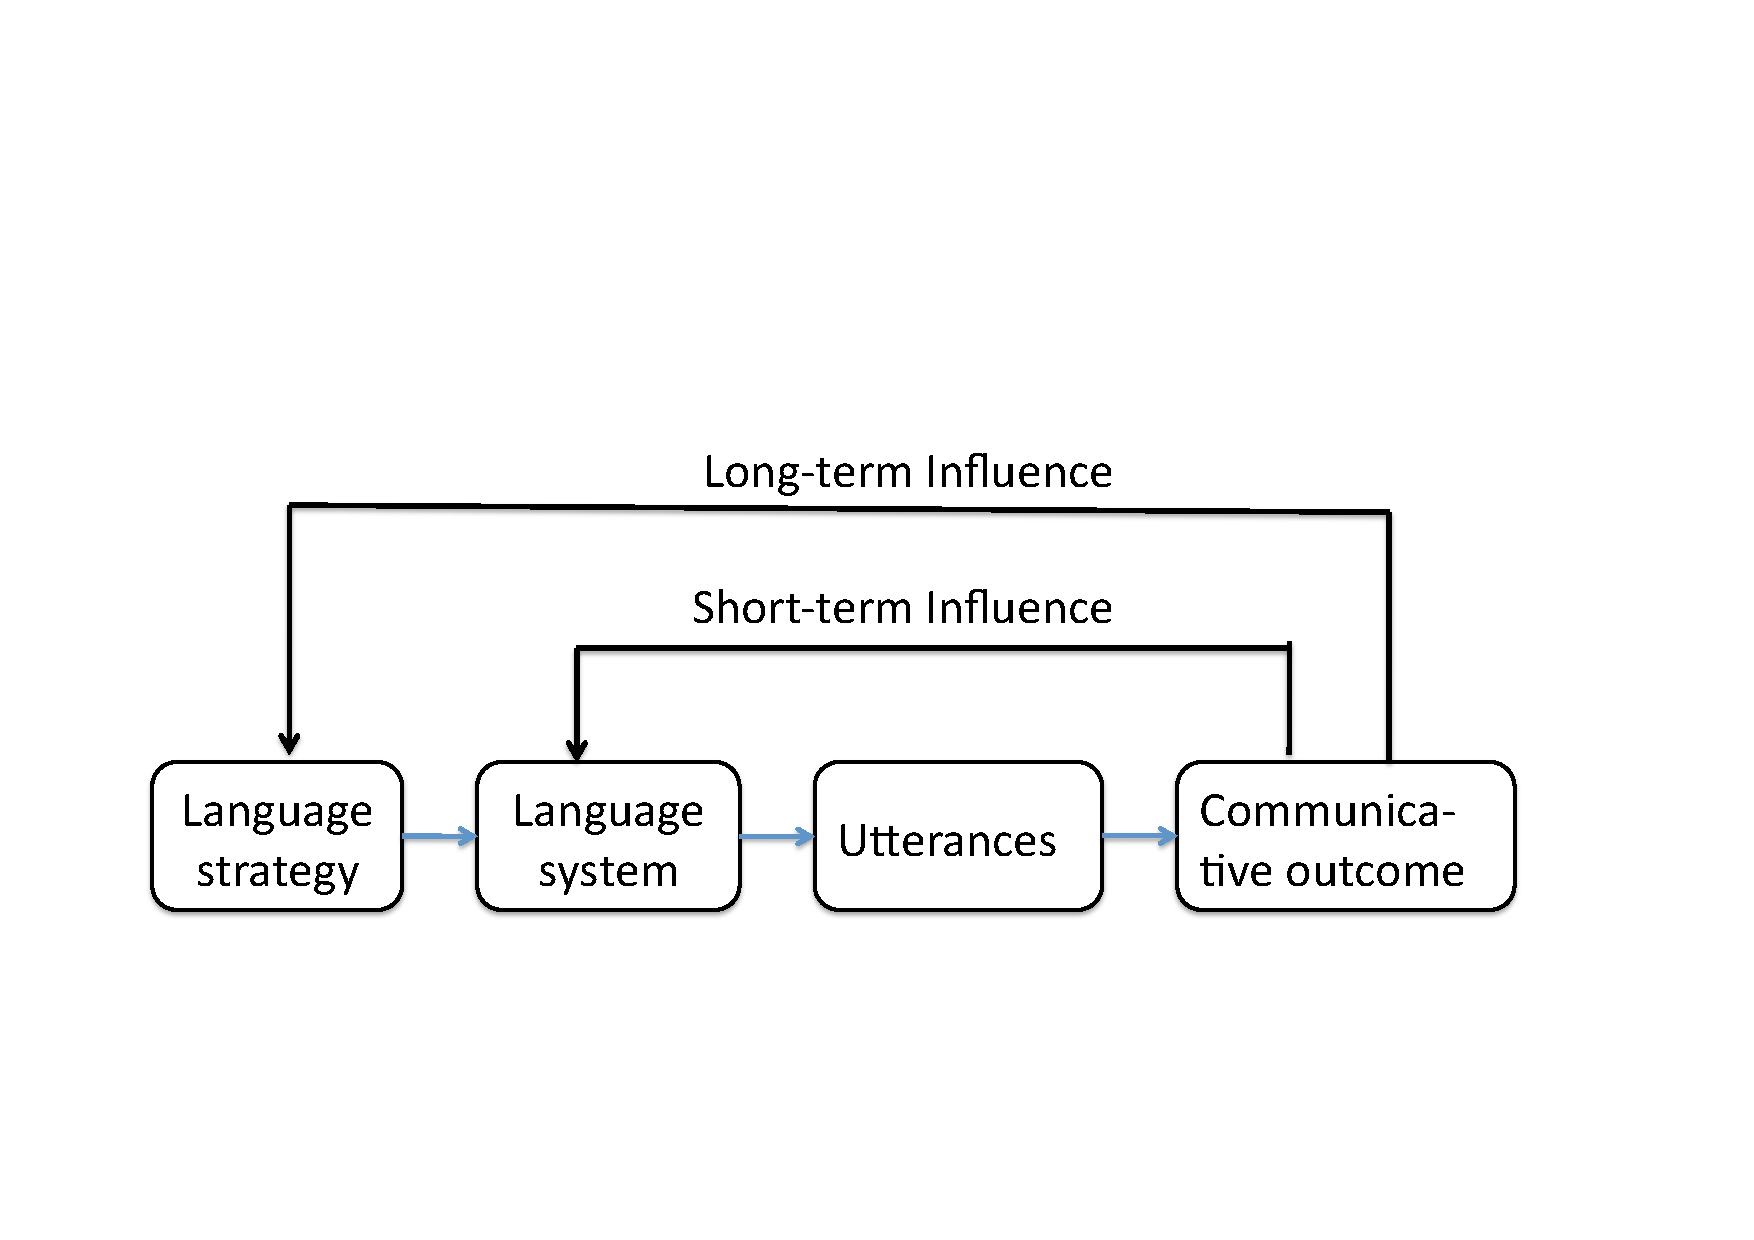
\includegraphics[width=0.7\columnwidth]{figs/select-strat}
\end{center}
\caption[Selective pressures on language systems and strategies]{The fitness of utterances for communication affects both the language
system and the language strategy. The effect of the success of a single utterance 
on the language strategy is smaller which leads to slower change on the level 
of the strategy. (Figure adapted from \citealp{steels2011self-organization})}
\label{f:strategy-system-selection}
\end{figure}



\begin{description}
\item[Selection]\index{selection}
Selectionism rests on two principles: \emph{generation} of
possible variants and \emph{selection} of variation based on fitness. 
The most important factor in determining the fitness of a 
particular language strategy, but also
of a particular language system, is \emph{communicative success}.
A communicative interaction between two interlocutors is successful if the
communicative intention of the speaker is reached. For instance, if the speaker
wanted to draw attention to some object, the communication is successful if the
hearer pays attention to that object. Communicative success drives selection\index{selection}
on the levels of the language system, but also on the level of language
strategies (see Figure \ref{f:strategy-system-selection}). 

Variation occurs in the systems for two reasons. 
First, agents are actively trying to solve 
problems in communication \citep{steels2000language}\index{Steels, L.}. 
Agents introduce new categories, 
new words and grammar when they detect problems that they 
cannot solve using the current
language they know. Second, language is an inferential 
communication system \citep{sperber1986relevance}\index{Wilson, D.}\index{Sperber, D.} which means 
that the information provided in an utterance is often 
incomplete and ambiguous. Interpreting phrases is an active 
process in which the hearer
is fusing information from the context, from the dialogue 
and his knowledge about the language 
to arrive at the best possible interpretation. In this process 
of course hearers might interpret
the utterance differently then intended. This is the 
second source of variation.

\item[Self-organization]
\cite{steels2011self-organization}  assumes that selection\index{selection} is not enough to explain 
language change and proposes another driving force in the evolution of language: 
self-organization\index{self-organization} -- a concept used to account for complex 
phenomena in physical and biological systems. In short, self-organization is a way to explain 
how global structure arises out of local interaction of subunits \citep{camazine2003self}\index{Camazine, S.}\index{Franks, N. R.}\index{Bonabeau, E.}\index{Sneyd, J.}\index{Deneubourg, J. L.}\index{Theraula, G.}. 
An example from biology for self-organization is swarm behavior in a school of fish. 
Each individual fish locally controls its behavior based on the estimation of the 
position and direction of its immediate neighbors. On the global level this leads to 
consistent swarm behavior. Self-organization is typically seen as a complementary 
mechanism to selection\index{selection}, although there is some discussion 
on how to reconcile the two mechanisms. 
\cite{kauffman1993origins}\index{Kauffman, S. A.}, for instance, proposes the following idea. 
Local components and the interaction rules are determined by selection\index{selection}, whereas the global emergent behavior is explained using self-organization. 
Applied to the swarm behavior this means that the anatomy of fish as 
well as the perceptual feedback loop are a product of natural selection. 
The global emergent swarm behavior is the product of self-organization. \index{selection}

Similar to swarm behavior, agents in a population evolving a language have
to achieve global coherence in the language they use. Each agent has its own 
private representations of the language that they speak and they can 
adjust their own representations based on local interactions with peers. 
How, from local interactions, agents can agree
on a globally shared communication system is the problem of alignment\index{alignment}.
Psychologists have found that interlocutors align on all levels of linguistic processing
even over the course of a few interactions, i.e., dialogue
\citep{garrod1994conversation,pickering2004toward}\index{Garrod, S.}\index{Doherty, G.}\index{Pickering, M. J.}.
Similar mechanisms applied over a long time span are required for driving populations 
to self-organize a sufficiently shared communication system 
\citep{steels2002bootstrapping}\index{Steels, L.}\index{Kaplan, F.}. 

\item[Recruitment]\index{recruitment}
The last problem for an account of how languages change in the 
\emph{selectionist theory of language evolution} is the problem of language strategy
generation. The hypothesis is that language strategies are recruited by assembling
basic cognitive operations\index{cognitive operation} \citep{steels2007recruitment}\index{Steels, L.}. For instance, an 
absolute spatial conceptualization strategy\index{conceptualization strategy}
involving distinctions such as ``north'' and ``south''  consists of basic categorization
mechanisms and the ability to track ones own direction. The two abilities are assembled
into the strategy which encompasses the different absolute spatial distinctions.
The process is called \emph{recruitment}\index{recruitment} because the cognitive mechanisms which
are assembled could, in principle, have evolved or could be learned independently 
from language. 

\item[Co-evolution] \index{co-evolution}
One of the tenants of the theory of linguistic selection is that syntax and semantics co-evolve. 
The idea is that recruitment\index{recruitment} of conceptualization strategies and the invention of new
semantic distinctions and spatial relations trigger evolution of the syntax of a language
\citep{steels1997distinctions,steels1998synthesizing}\index{Steels, L.}.  
For instance, presumably when the absolute system in German emerged based
on a new way of construing reality, this at the same time triggered 
the invention of new words. 
\end{description}

\subsection{Evolutionary explanations}
In every science one has to define what counts as an explanation. 
This book is guided by what counts as an evolutionary explanation
in biology, ethology and psychology \citep{tinbergen1963aims,dunbar1998theory}\index{Tinbergen, N.}\index{Dunbar, R.}. 
In order to explain a complex trait from the evolutionary perspective 
one has to provide explanations on four different levels: \emph{function}, 
\emph{mechanism}, \emph{ontogeny} and \emph{phylogeny}.

\index{function}\index{ontogeny}\index{phyologeny}\index{mechanism}
\begin{description} 
\item[Function] An explanation for a particular behavior has to show what
the behavior is good for, i.e. what is its purpose. For Darwinian biology, 
the function of a behavior has to be explained in terms of its impact 
on survival or, more precisely, on the production of offspring. For evolutionary
linguistics this turns into the question of how a particular language system or a particular strategy
helps an agent to be more successful in communication. For example,
one can explain particular spatial language systems with respect to their ability
to help agents solve communicative problems in spatial navigation and 
spatial reference.

\item[Mechanism] Besides function, one has to identify the mechanisms that give rise 
to the behavior. 
This is actually called \emph{causation} by \cite{tinbergen1963aims}\index{Tinbergen, N.} 
and it refers to the cause and effect relations that generate a particular behavior. 
For instance, one can explain how aggressive behavior is generated by looking
at changes in hormone levels in an organism, e.g., testosteron causes aggressive behavior.
For spatial language this entails a detailed operational model of the 
production and parsing of spatial language.

\item[Ontogeny] The next question is how a particular behavior is acquired. To
answer this question one has to identify the developmental steps that
the behavior undergoes, but also what is the ontogenetic basis 
of the behavior. What is learned and what is instinct? For spatial language this 
requires insights into how spatial language is learned.

\item[Phylogeny] A fourth part of every evolutionary explanation has to
identify the evolutionary history of a behavior. What are
the sequential stages of evolution of a behavior? What are the prerequisites
of a behavior? How do evolutionary older behaviors influence 
the behavior under question? These questions have to be answered
with respect to the function of the behavior. In other words, one needs
explanations of how the behavior evolved to fulfill its current function. 
For language evolution scholars have to identify how a particular strategy 
evolved over time. Was it adapted from an older strategy? 
How did syntax and semantics of the language system under consideration co-evolve over time?
\end{description}

\section{Main hypothesis}
\label{s:intro-main-hypothesis}
This book provides experimental evidence for the theory of linguistic
evolution. The hypothesis is that \emph{spatial language syntax and 
spatial semantics co-evolve through a cultural process based on selection\index{selection}, 
self-organization and recruitment}\index{self-organization}\index{recruitment}. This book explores the hypothesis for 
the different components of spatial language: spatial relations, landmarks 
and perspective. Computational experiments
show the emergence of spatial relations, the negotiation of the use of landmarks
and perspective. I also explore different strategies for expressing
spatial conceptualizations: lexical and grammatical strategies.

\section{Contributions}
\label{s:intro-objectives}
This book provides detailed accounts of 
the function, mechanisms, ontogeny and phylogeny of spatial language. 
\begin{enumerate}
\item The first contribution is an explanation of the mechanisms behind spatial language
for German locative phrases in a complete reconstruction including
perception, semantic and syntactic processing. Once the mechanisms are in place,
we test the function and impact of components of spatial language in experiments
by removing the component in question and examining the effect the removal has
on communication.
\item The second contribution is to explain steps in the co-evolution\index{co-evolution} of spatial 
syntax and spatial semantics through computational models.
\end{enumerate}

This book follows a whole systems approach which allows us to define external 
criteria for the progress in each of the objectives. The defining moment for the 
underlying conception of language is communication. A communication system 
is \emph{successful} if it allows robotic agents to achieve 
their communicative goals such as drawing the attention to an object in the environment. 

% steps in the evolution of spatial language
\subsection{Evolutionary Stages}
\label{s:stages}
One way of understanding evolutionary processes is to try to identify
evolutionary stages. Over the years, different steps in the evolution
of language have been identified involving varying degrees of 
specificity \citep{bickerton1999language,jackendoff1999possible,steels2005emergence}\index{Steels, L.}\index{Jackendoff, R.}\index{Bickerton, D.}. 
All of these proposals, while differing in detail and the exact number of stages,
agree that language evolution starts at some pre-grammatical stage and 
increases in complexity to the form of language, in particular, grammar 
that we see today. Obviously any evolutionary account of language has to show how 
the current state of complexity of language can be traced back to earlier simple stages. 


\begin{figure}
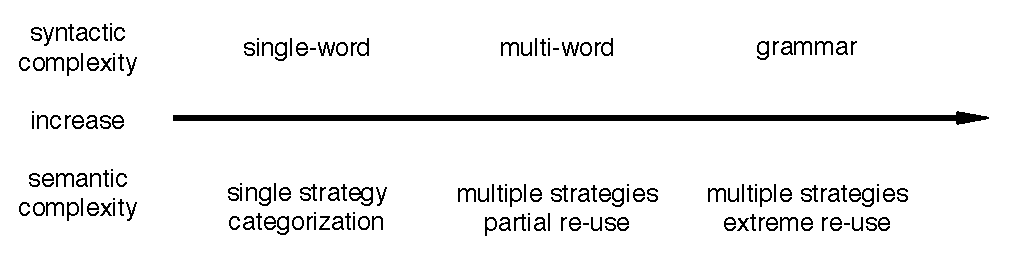
\includegraphics[width=1\columnwidth]{figs/co-evolution-complexity}
\caption[Co-evolution of syntactic and semantic complexity.]{Co-evolution\index{co-evolution} of syntactic and semantic complexity.}
\label{f:co-evolution-complexity}
\end{figure}

This book orients itself alongside \cite{steels2005emergence}\index{Steels, L.}, who proposes
a number of stages of complexity which are relevant for this book:
\emph{single-word utterances}, \emph{multi-word utterances}, and \emph{grammatical utterances}
(see Figure \ref{f:co-evolution-complexity}). 
 
\begin{description}
\item[Single-word utterances] In this stage agents utter single words that pertain to a particular concept
or category used for discriminating objects. Examples for spatial language include utterances that 
directly refer to spatial regions such as \textit{links} (`left') or \textit{n\"ordlich} (`north').
When agents can only express themselves using a single word, this single word necessarily encodes
the complete conceptualization strategy. For instance, which landmark or perspective is used for conceptualization is holistically coded in the single word. Since there is no additional information 
about which conceptualization strategy the term is referring to, agents have to implicitly agree on 
the precise spatial construal the term is referring to. This limits the re-use of spatial categories 
in different spatial conceptualization strategies because agents have no way of 
disambiguating the use of the same spatial relation in different strategies.
\item[Multi-word utterances] Single-word communication systems are not very flexible. 
There is no compositionality and particularly there is no re-use. In German, for instance,
projective relations can be used with different landmarks. In the multi-word utterance stage 
agents can express different constituents by using a number of lexical items. 
Besides expressing the spatial category used, agents can also 
mark landmarks. An example utterance is \textit{links Kiste} (`left box') which is used 
to signal that the region left of the box is meant.
\item[Grammatical utterances] When we look at natural language, we can see 
that the \emph{same} constituents can be part of different conceptualization strategies. 
Imagine an utterance like \textit{Kiste link} (`box left') without the grammatical information, in particular, 
without word order and lexical class information. In that case a hearer does not know whether 
\textit{link} is an adjective or an adverb. This syntactic underdetermination has consequences for 
the semantic interpretation. If the phrase is interpreted as an adjective noun phrase as in 
\textit{linke Kiste} (`left box'), the spatial category acts as a modifier on the set of boxes. If the 
spatial relation is interpreted as an adverb, then box might be a landmark and the whole phrase 
denotes a region next to the landmark as in \textit{links der Kiste} (`to the left of the box').
Grammar signals the difference in these two semantic interpretations and
disambiguates the conceptualization strategies. Consequently, agents equipped with grammatical
strategies can disambiguate even more strategies and consequently, they can be more expressive.
\end{description}

The goal of this book is to identify, implement and test the mechanisms that drive 
the evolution of language on \emph{each} of these stages. The mechanisms 
we are interested in are not descriptions of the phenomena but mechanistic explanations 
which identify the computational and cognitive components
that enable robotic agents to self-organize communication systems.
The procedure to find and validate mechanistic explanations is to
\begin{enumerate} 
\item hypothesize \emph{invention}, \emph{adoption} and \emph{alignment}\index{alignment} operators for the syntax and semantics
according to each stage of complexity,
\item equip agents with these operators,
\item test the evolutionary dynamics in populations of equipped agents,
\item measure the communicative success, adaptivity and expressivity.
\end{enumerate}
\index{invention}\index{adoption}
Invention, adoption and alignment\index{alignment} operators are the backbone of the evolutionary models 
of this book. For instantiating the theory of linguistic selection\index{selection} one has to identify 
agent-level mechanisms that orchestrate the global behavior of the population. The mechanisms 
can be classified into the following three classes.
\begin{description}
\item[Invention operators] Invention is the process of introducing variation 
into the system by inventing a new spatial relation or a word or even grammar
in order to solve a problem in communication. A speaker, for instance,
who is unable to discriminate an object might introduce a new spatial
category to be able to identify the object. Subsequently, he might invent
a new word to be able to express the new spatial category.
Invention operators introduce variation and novelty into the system.
\item[Adoption operators] Adoption is the process by which an
agent acquires a new word, a new spatial relation or a new piece of grammar.
Acquisition is carried out by hearers in interactions when they observe
new items that they are unable to process.
Adoption is another source of novelty and variation. An agent that
picks up a new word might have a different idea of what that word
means than the speaker actually intended. 
\item[Alignment operators] Invention is local to an interaction. When two
agents communicate and one of them invents a new word, this word
might be acquired by the interlocutor, but the knowledge about this 
word is still local. Alignment\index{alignment} operators orchestrate the self-organization\index{self-organization}
of the system and the global alignment of language.
\end{description}


\subsection{Co-evolution of syntactic and semantic complexity}
In each stage, syntactic complexity co-evolves\index{co-evolution}
with semantic complexity (see Figure \ref{f:co-evolution-complexity}). 
Syntactic complexity rises because the number of words
per utterance increases (from the single-word stage to the multi-word stage) 
and because syntactic categorizations such as word order, morphology, 
agreement become important (from multi-word to grammar).

The notion of semantic complexity is harder to define. Obviously
German spatial language is complex. But why does this seem obvious? 
What are the properties that make it a complex semantic system? For this book, 
complex semantics is defined with respect to spatial language as: the language supports a large 
number of conceptualizations of a spatial scene. There are two factors influencing 
the complexity of the space of possible conceptualizations of a spatial scene.

\begin{description}
\item[Number of relations] A first level of semantic complexity
is related to the number of spatial categories. For the part
of German locative phrases considered in this book, we already have 
12 spatial relations. But there are, of course, many more relations not considered
in this book such as  dynamic relations. 
For some scholars this is the only definition of semantic complexity (compare 
\citealp{schoenemann1999syntax}\index{Schoenemann, P.}).
\item[Number of conceptualization strategies]
A second notion of semantic complexity is the number of
conceptualization strategies a language supports. German, for instance, supports
many different categorization systems: projective, e.g. \textit{links} (`left') or \textit{rechts} (`right'), 
proximal, e.g. \textit{nah} (`near') and \textit{fern} (`far'), and absolute, e.g. \textit{n\"ordlich} (`north') 
and \textit{s\"udlich} (`south'). This is one aspect. The other aspect is that
these systems are part of different conceptualization strategies. 
Examples of this re-use were already given earlier with respect to adjectives and adverbs.
\end{description}

\section{Structure of the book}
\label{s:intro-structure}
This book is structured into three main parts besides this introduction 
and the conclusion. Part \ref{p:embodied-language-games} explains the interaction
model and the technical systems needed for studying spatial language.
Part \ref{p:german-locative-phrases} deals with objective number one and details the reconstruction
efforts for the German locative system. In Part \ref{p:spatial-language-evolution} I detail how spatial
language evolves based on the model of evolutionary stages.


\subsection{Part I: Spatial language games and technical background}
\index{spatial language game}
\subsubsection{Spatial language games}
Spatial language occurs mainly in interactions of individuals in spatial scenes.
To research spatial language in such a communication-based approach
to language a number of things need to be in place. We need a model of 
interactions in spatial scenes. This is the topic of Chapter \ref{s:spatial-language-games} which 
introduces \emph{spatial language games} which are routinized interactions
consisting of defined roles for interlocutors -- speaker and hearer. 
The chapter explains the basic interaction scheme and the 
linguistic and non-linguistic behaviors that define a spatial language
game. 

\subsubsection{Embodied cognitive semantics with IRL}
In order to achieve the objectives of this book, we need computational 
formalisms that support the reconstruction and evolution investigations. 
One of such formalisms in part developed for this book is the
\emph{Incremental Recruitment Language} (IRL). IRL is (a) a formalism
for representing semantics, (b) a set of planning algorithms for automatic
conceptualization and interpretation, and (c) a set of tools that make
semantics an open-ended adaptive system. Chapter \ref{s:irl} 
introduces the formalism and the technology behind it.

\subsubsection{Construction grammar with FCG}
Another important backbone of the investigations is Fluid Construction 
Grammar (FCG). FCG is a formalism for representing and processing linguistic 
knowledge. Chapter \ref{s:fcg} details how mappings from semantics to syntax 
are implemented using FCG and gives an example of processing a simple phrase.\index{Fluid Construction Grammar}

\subsection{Part II: Reconstructing German locative phrases}
To ground the modeling efforts in sufficient knowledge of a real spatial language system, 
I decided to reconstruct a part of German spatial language -- German locative 
phrases. The second part of this book reconstructs the syntax and semantics 
of German locative phrases. The part starts out with an in-depth look at
German locative spatial language as a natural language phenomenon. Chapter
\ref{s:german-spatial-language-introduction} gives more examples of the syntactic variety and the connection to the
space of conceptualization strategies supported in German locative phrases.
This sets the scope for the reconstruction effort, but also identifies a number
of processing issues that the reconstruction has to deal with in order to be successful.

\subsubsection{Spatial semantics}
The following chapter details the operationalization of spatial semantics. 
Chapter \ref{s:german-space-semantics} the basic semantic building blocks of German locative phrases
and discusses how they work together to make up the complex 
semantics of spatial scenes.  

\subsubsection{Syntactic processing}
A close look at German locative phrases reveals a number of interesting phenomena.
Most importantly it uncovers the tight relationship between spatial 
syntax and spatial semantics. Chapter \ref{s:german-locative-phrases-syntax} 
explains how FCG can be used 
to model the tight connection between the words and grammatical 
relations observed in German locative phrases and the world of spatial semantics.
These mappings are interesting because they pose particular challenges to
the organization of linguistic processing. The re-use of the same spatial categories
in different strategies for conceptualizing reality and their syntactic expression
requires sophisticated mechanisms for dealing with many-to-many mappings 
in language. Another important issue is how to deal with the case
system of German. All of these aspects of linguistic processing are
discussed in Chapter \ref{s:german-locative-phrases-syntax}.

\subsubsection{Conceptualization of spatial scenes}
Spatial scenes do not come a priori labeled, categorized and construed.
Agents have to autonomously conceptualize reality given the
particular communicative goal they have. 
Chapter \ref{s:german-locative-phrases-semantic-processing} deals with the problem
of conceptualization which is the problem of how to construct semantic
structure that is helpful in reaching communicative intentions. The chapter
gives an overview of different factors influencing the conceptualization
of spatial scenes and compares different implementations of 
spatial conceptualization.

\subsubsection{Integrating syntactic and semantic processing}
The last chapter of this part reports on the integration of syntax, semantics 
and conceptualization. One of the issues that can be studied in an approach
like mine is \emph{semantic ambiguity}\index{semantic ambiguity} which refers to the fact that natural
language is often ambiguous with respect to the precise interpretation
of a phrase. But humans are very strong in communicating even though 
language only encodes hints at how to conceptualize reality. The key
is that humans integrate the sparse information communicated in utterances 
with knowledge about the current context of the interaction. 
Chapter \ref{s:german-locative-phrases-syntax-semantics-integration}
explains how one can operationalize this process of disambiguation through
the context using the conglomerate of systems for linguistic and semantic
processing as well as perception.



\subsection{Part III: Spatial language evolution}
Finally the book turns to evolution in the third part. The organization of this part
orients itself along the stages of complexity introduced earlier. There are two
parts on single-word utterance systems, followed by a chapter on multi-word utterance
systems. The part closes with a chapter on the evolution of grammatical structure.

\subsubsection{Acquisition and formation of basic spatial category systems} 
The first chapter in this part explains how the basic building blocks of 
spatial language -- spatial relationships and corresponding words --  
become shared in populations of agents.
This corresponds to complexity stage one -- single words. The goal of the chapter is 
to define the language strategies necessary for forming single-word spatial language systems. 

Single-word spatial language systems are built by a particular strategy of 
conceptualizing reality which includes a priori commitments to certain reference 
objects, frames of reference and perspectives on the scene. The chapter shows how a 
language strategy which is a combination of a particular strategy for conceptualizing reality 
plus the necessary invention operators for basic spatial categories build the language systems 
that allow agents to communicate successfully. Language strategies are tested in two 
scenarios -- \emph{acquisition} and \emph{formation}. In acquisition a learner agent has to pick 
up the spatial language system spoken by a tutor. In formation all agents start from scratch 
and progressively develop categories and lexical items.

The most important influence on what kind of language system emerges is the 
language strategy. The chapter details different language strategies 
necessary for building proximal, projective and absolute systems which encompass
dedicated invention, adoption and alignment operators as well as the different 
conceptualization strategies. The success of the learning operators and the 
conceptualization strategy is tested in experiments where populations are fitted with a 
particular strategy. The resulting languages spoken by individual agents are analyzed with 
respect to communicative success and how similar they are to each other. 

Another important factor influencing the emerging 
language system are environmental conditions. The chapter studies the impact of 
environmental conditions systematically by manipulating environmental features 
such as global landmarks or the statistical distribution of objects. 

Obviously, natural languages support many conceptualization strategies at the same time.
German, for instance, simultaneously has a proximal, a projective and an absolute system. 
So one can ask what happens when agents are simultaneously operating 
different strategies. I hypothesize that agents need additional cognitive mechanisms 
for choosing between different strategies and that choosing a strategy can be realized
using the \emph{discriminative power} of each strategy in a particular context. 
When an agent has to invent a new category they use the strategy that is most
discriminating using a new category. Experiments show that this principle
allows agents to build multiple language systems at the same time.
Lastly, the chapter also studies the impact of different environmental 
layouts on formation of language systems for interacting strategies.

\subsubsection{Origins and alignment of spatial conceptualization strategies}
Chapter \ref{s:strategies} deals with the emergence and 
alignment of conceptualization strategies.
When one compares different languages of the world it becomes clear that many languages 
differ in the kinds of conceptualization strategies they support. Some languages 
solely use an absolute system, others can use intrinsic and relative systems and so on
and so forth. Consequently, the evolution of spatial language is intricately connected to the 
origins and evolution of spatial conceptualization strategies. The chapter shows that
conceptualization strategies are organized in a process of recruitment, selection\index{selection} and 
self-organization\index{self-organization}\index{recruitment}. 

% competition
To explain conceptualization strategies from the viewpoint of the theory of linguistic
selection\index{selection} is to explain (a) how different conceptualization strategies are created
and (b) how they are selected for in communication. Competition is an important aspect
of selection. Obviously environmental conditions and communicative success 
are main influences on which strategies are selected for because they are more successful. 
The chapter proposes alignment operations that update and track the score
of conceptualization strategies so that agents can locally align in their
interactions. I show that these operators lead to global convergence
of the population on using single conceptualization strategies.
The chapter studies competition of different strategies for landmarks and 
frames of reference and shows that with the right alignment strategy
agents can agree on using a particular conceptualization strategy while
co-evolving a lexicon and ontology of spatial relations at the same time.

Besides selection\index{selection} the theory has to explain how conceptualization
strategies are created. This is were the idea of recruitment\index{recruitment} comes into play.
Conceptualization strategies are assemblies of cognitive operations\index{cognitive operation}. For instance,
an absolute strategy consists of a particular way of applying spatial categories
plus the computation of a global landmark. Recruitment\index{recruitment} is the process
of drawing from the pool of cognitive operations\index{cognitive operation} and assembling and packaging
them so that the complete structure for conceptualization can be scored and 
the score updated and tracked. In a second set of experiments creation
and competition of strategies are studied together.

\subsubsection{Multi-word lexical systems for expressing landmarks}
Single-word utterance systems are limited in how much information can be conveyed
in them. Upon hearing a single term it is hard to decide what conceptualization
strategy was it part of. Which landmark is used? Which perspective
did the speaker have in mind? These are questions that cannot be decided
by just looking at a single word, unless of course the word is known and always
refers to the same landmark and the same conceptualization strategy.
When we look at human language we see a lot of re-use of spatial relations.
Absolute, projective and proximal relations in German can be used with
different landmark objects. Chapter \ref{s:multi-word} examines what mechanisms
are needed for agents to mark landmark objects using lexical items 
while at the same time co-evolving a lexicon and ontology of spatial relations. 
Once these mechanisms are in place success of such extended lexical systems
can be studied and compared to systems which only support a single
conceptualization strategy.

\subsubsection{Grammar as a tool for disambiguating spatial phrases}
The part on language evolution of this book is concluded by Chapter \ref{s:grammar} that examines
the role and evolution of grammatical language. 

Lexical systems which are all systems studied up to this point in the book, 
have considerable shortcomings. One can study the effect grammar has by removing
grammatical knowledge from the German locative grammar implemented for this
book. The results presented in Chapter \ref{s:grammar} show that agents operating a 
German locative system without grammar have significantly lower communicative 
success. I show that environmental conditions and diverging perspective on the scene can increase 
the drop in communicative success. The lack of grammar increases \emph{semantic
ambiguity} of phrases which means that the number of possible interpretations
of a phrase escalates. As a consequence, the number of wrongly interpreted topics enlarges
as well.

Given such a clear communicative advantage for having grammar, one can 
study the necessary operators that enable agents to develop a grammar for 
disambiguating spatial phrases. This is the topic of the second part of 
Chapter \ref{s:grammar} which reports on the precise implementation of these operators.
I test the operators in multi-agent experiments which prove that the 
hypothesized invention, learning and alignment operators allow agents 
to become increasingly more successful in communication because 
they develop an effective grammatical communication system.

%
% \bibliographystyle{diss}
% \bibliography{papers,space}
% \end{document}

% 2. Background
\part{Spatial language games and technical background}
\label{p:embodied-language-games}
%\documentclass[a4paper,9pt,fleqn,notoc]{diss}
%\renewcommand{\includegraphics}[1][1]{} 
%\begin{document}


%%%%%%%%%%%%%%%%%%%%%%%%%%%%%%%%%%%%
\chapter{Grounded Spatial Language Games}
\label{s:spatial-language-games}
\index{spatial language game}
\begin{figure}
\begin{center}
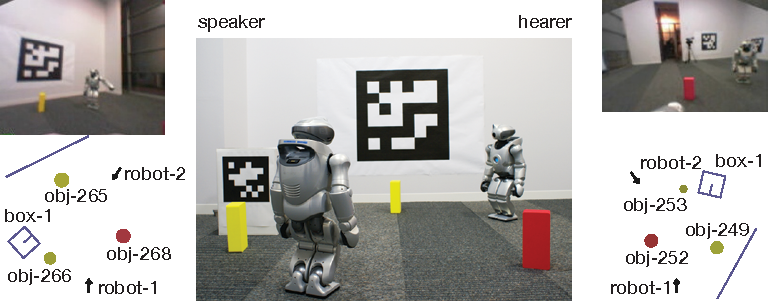
\includegraphics[width=1.0\columnwidth]{figs/space-scene-2-small}
\end{center}
\caption[Example spatial setup]{Example scene. 
Two robots autonomously perceive and act in an office 
environment that contains different types of objects. Both 
robots autonomously create world models reflecting the state 
of the environment (see bottom left and right schematics), that 
include objects with spatial and color properties, the carton boxes 
as well as the robots.}
\label{f:scene}
\end{figure}

Language does not occur in a vacuum. Spoken language occurs in physical,
situated interactions when two interlocutors meet with specific
communicative intentions. This chapter explains the basic social interactions 
at the center of the approach to language. Physical robots meet in communicative
encounters and try to reach communicative goals within real world settings. 
Taking such a radical approach to the study of language is grounded in a number of
social and perceptual mechanisms. Here I look at the prerequisites for 
the computational models discussed later in this book.

Figure \ref{f:scene} shows such an encounter of
two humanoid robots in which one of the robots, the speaker, has the goal
of drawing the attention of the hearer to some object in the environment using language.
Such interactions are called \emph{language game} \citep{steels2001language}\index{Steels, L.}.
Language games are routinized interactions between two members of 
a population. The game combines a particular script for the interaction, the linguistic
information transfer and extra-linguistic feedback about the success of the interaction.
Here is an example of a language game called the \emph{spatial language game}.


\begin{enumerate}
\item The language game starts by randomly drawing two agents from the population. 
One agent is randomly assigned the role of speaker, the other is assigned the role
hearer.
\item The agents establish joint attention and perceive the scene.
\item The speaker chooses an object from the perceived context as the object
he wants to draw the attention of the hearer to.
\item The speaker produces an utterance that he thinks draws the attention to the object.
\item The speaker passes the utterance to the hearer.
\item The hearer interprets the utterance and tries to find the object that the speaker
might have in mind. 
\item The hearer points to the object he thinks the interaction was about. If he was unable 
to interpret a topic, he signals this by shaking his head.
\item The speaker interprets the pointing. If the object pointed to by the hearer
is correct, he signals this by noding. If the hearer pointed to the wrong object or
did not point at all, the speaker
points to the topic he wanted to draw the attention to.
\end{enumerate}


\begin{figure}
\begin{center}
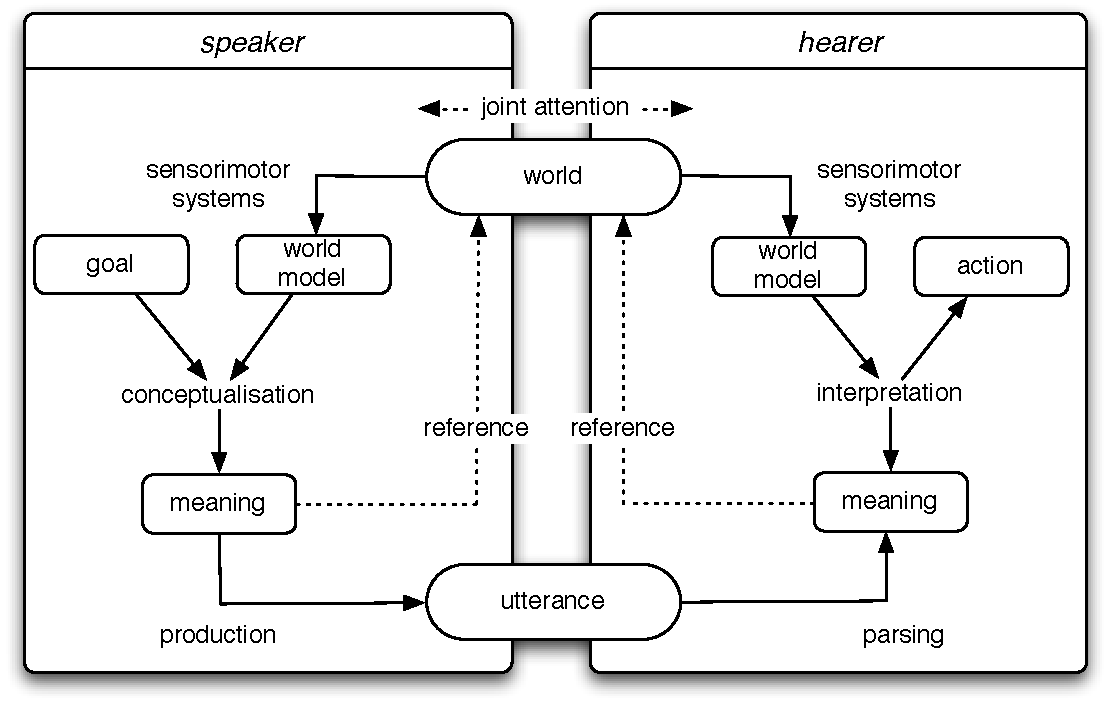
\includegraphics[width=0.9\columnwidth]{figs/semiotic-cycle}
\caption[Semiotic cycle]{\index{semiotic cycle}The semiotic cycle is a model of situated communicative interactions between 
two interacting agents.}
\end{center}
\label{f:semiotic-cycle}
\end{figure}

To study language in a real world  setting requires to fully spell out 
all components involved in the interaction.
Besides social mechanisms agents need operational systems for perceiving
the world, as well as the construction and interpretation of utterances. 
Figure \ref{f:semiotic-cycle} shows a schematic view of the systems
involved in production and parsing, conceptualization and interpretation. 
Both agents independently process sensorimotor data stemming from
the onboard cameras and proprioceptive sensors in order to construct 
world models\index{world model} of the environment 
\citep{spranger2008grounded,spranger2012perception}\index{Spranger, M.}. 
Based on the particular communicative goal and the current state of the 
world represented in the world model, the speaker conceptualizes a meaning 
which is then rendered into an utterance by the language system. 
The hearer parses the utterance to determine its meaning and 
interprets it with respect to his current model of the world in order 
to infer the speaker's communicative goal and, for instance, 
perform a desired action. The system used for conceptualization
and interpretation are explained in detail in Chaper \ref{s:irl}.
The system for producing and parsing utterances is treated in
Chapter \ref{s:fcg}. 
The following sections focus on the necessary prerequisites for 
language production, parsing and evolution in terms of social mechanisms and 
perceptual processing.

\section{Perception}\index{perception}
\label{s:perception}
The environment that robots interact in is equipped with four kinds of objects
that were carefully chosen to pick out special features relevant for spatial language:
\emph{blocks}, \emph{boxes}, \emph{wall markers} and the \emph{robots} themselves 
(see Figure \ref{f:scene}). 
\begin{description}
\item[Blocks] Are the colored brick like objects. They are typically of the same color.
Agents perceive these objects as having a certain distance from their 
egocentric coordinate systems originating in the robot's body.
\item[Boxes] The environment also features card boxes which have 
particular markers on their sides. These markers are perceived by the sensorimotor 
systems as distinct sides of the object. The perceptual systems
perceive them as having a particular distance and orientation with
respect to the robot's coordinate system. 
\item[Wall markers] Figure \ref{f:scene} shows that the same markers
used for the carton boxes can also occur on the wall.
Cardboard boxes introduce a geocentric orientation on the scene.
\item[Robots] Robots also establish the position of the interlocutor in
each interaction. Every robot tracks the position and orientation of the
other robot in his environment.
\end{description}


Before a language game starts the robots perceive their
environment. The robots are endowed with perceptual systems 
for recognizing and tracking the objects in their environment.
These systems continuously build up \emph{world models} of the environment
consisting of sets of objects. The objects are characterized by continuous
real-valued features such as color, position and orientation but also
width, height and length. The perceptual system also provides a basic
grouping of objects into classes such as robots, blocks and boxes and wall markers. 
The following is the world model built by the agent to the left in Figure
\ref{f:scene}. It includes the other robot ({\footnotesize\texttt{robot-2}}), the
landmark ({\footnotesize\texttt{box-1}}) and the colored blocks ({\footnotesize\texttt{obj-265}},
{\footnotesize\texttt{obj-266}} and {\footnotesize\texttt{obj-268}}):
\label{world-model-example}
\begin{footnotesize}
\begin{verbatim}
((robot-1 :type robot :x 0.0 :y 0.0 :orientation 0.5)
 (robot-2 :type robot :x 1461.65 :y -351.24 :orientation 0.9)
 (box-1 :type box :x 513.0 :y 891.67 :orientation 0.36 
        :width 320.0 :height 450.0 :length 310.0)
 (obj-265 :x 1454.74 :y 248.72 :z 0.0 :width 59.75 
          :height 235.99 
          :average-y 128.0 :stdev-y 26.49 :min-y 51.0 
          :max-y 199.0 :average-u ...)
 (obj-266 :x 285.0 :y 549.02 :z 0.0 ...)
 (obj-268 ...)
 (box-wall :orientation 0.36))
\end{verbatim}
\end{footnotesize}


Each robot constructs perceptual representations of the objects in its
immediate surroundings from the raw sensations streaming from the
robot's sensor. Each type of object in the environment is tracked
by a dedicated perceptual system. In general, processing of 
the different object classes is  a three step process.
First, low-level vision routines process raw camera
images to yield basic \emph{percepts} -- these are connected regions that
differ from the background of the environment or are related to 
the patterns distributed on the boxes and wall markers.
Second, these regions are tracked in subsequent
camera images. In order to do so, the vision system needs to establish a
correspondence between an internal \emph{model} and the image
regions that refer to the same physical object, a process known in
robotics as \emph{anchoring} \citep{coradeschi2003anchoring}\index{Saffiotti, A.}\index{Coradeschi, S.}. 
I use state estimation techniques from robotics, e.g. \emph{Kalman Filters} 
\citep{kalman1960linear}\index{Kalman, R. E.}, 
for maintaining such persistent models. Third, the vision system 
fuses information from the proprioceptive sensors of the robot
the visual information to encode a set of visual properties about each object. 
In this particular setup these properties are the position and orientation of objects, 
an estimated width and height and color information. In the experiments 
discussed in this book only position and orientation are relevant. 
Most importantly, the perceptual systems only track objects on the ground. 
The position and orientation of objects is encoded in 
a two dimensional \emph{egocentric} coordinate system which has 
its origin between the two feet of the robot facing to the front of the 
robot. \cite{spranger2008grounded}\index{Spranger, M.} gives more detail on the 
perceptual systems.

The experiments reported on in later sections require that agents play many
language games. In order to speed up the process of a game and in order to
do repeatable, manipulatable experiments, data from spatial scenes\index{spatial scenes}  such as the one 
in Figure \ref{f:scene} are recorded and stored. The output of the perception
system of more than 800 spatial scenes with different spatial configurations 
has been collected and can be accessed by artificial software agents without 
the agents required to run on physical robots.
A spatial language game can be enacted on such stored scenes as if robots 
were perceiving the scene at the very moment they are playing a particular 
language game.

Figure \ref{f:spatial-scenes-1} shows different spatial scenes. Each spatial scene 
consists of a world model for each of the two robots recorded from the position of 
each robot. Scenes are grouped into data sets with similar characteristics
with respect to perspective on the scene, the number of objects and
the availability of boxes and wall markers. For instance, in some data sets the perspective of interlocutors is similar (see Figure \ref{f:spatial-scenes-1} for 
examples from one data set), i.e., robots
are looking at the scene from the same position and there are few objects.
Figure \ref{f:spatial-scenes-2} shows examples from different data sets.

\begin{figure}
\begin{center}
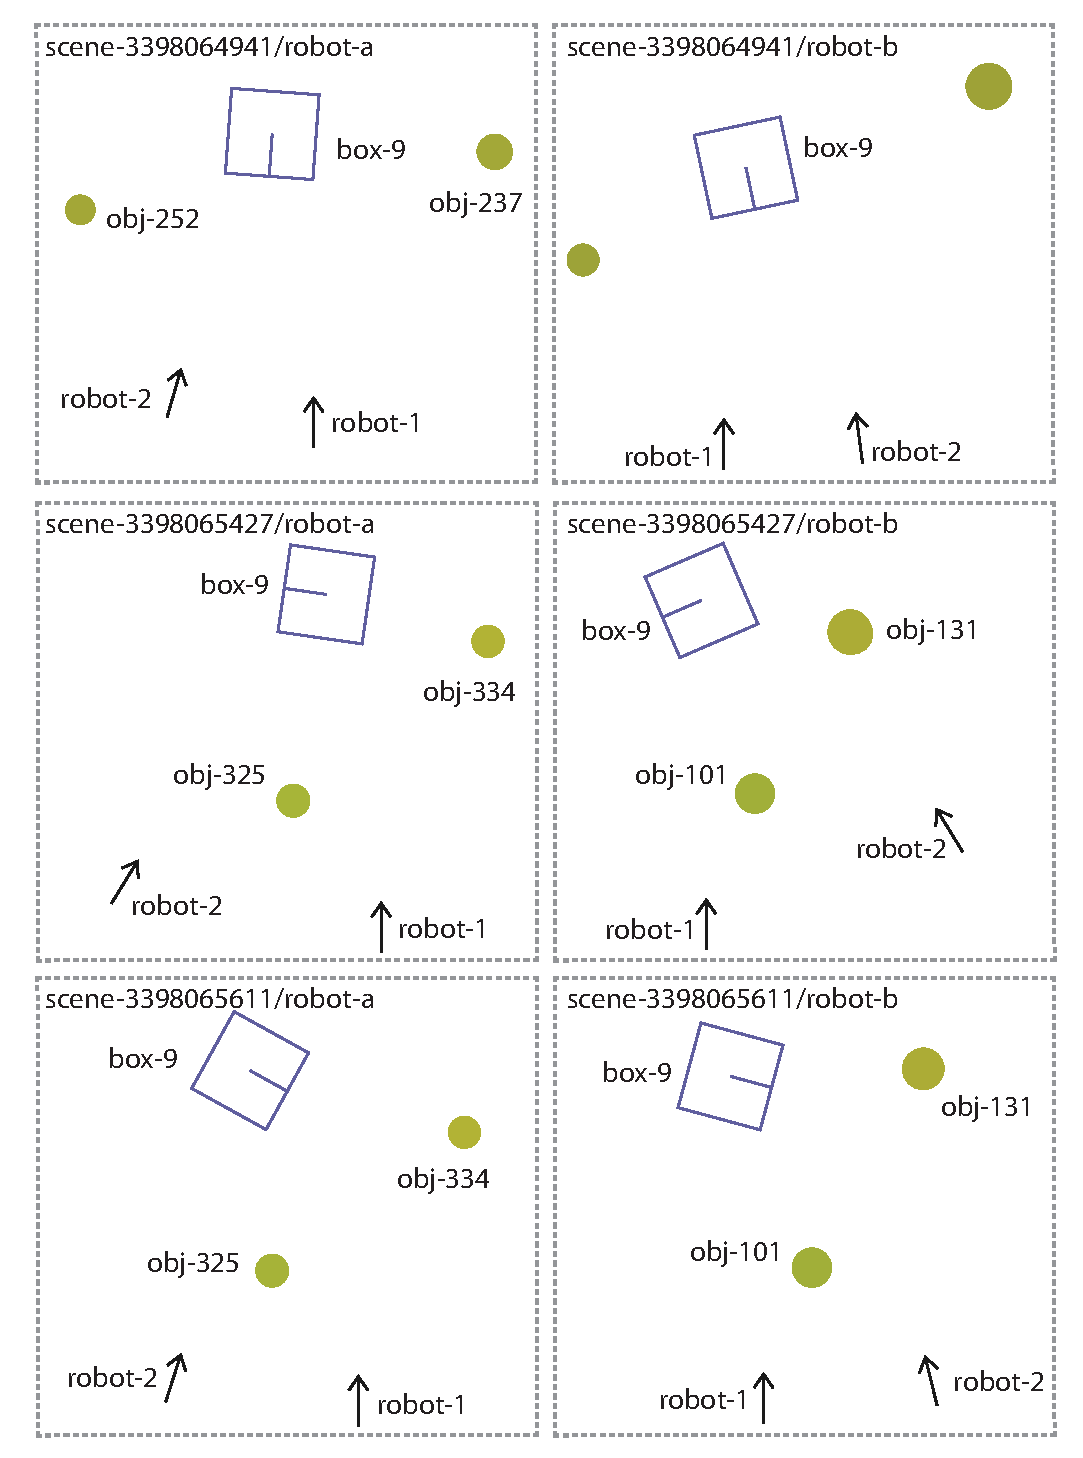
\includegraphics[width=0.8\columnwidth]{figs/spatial-scenes-overview-1}
\end{center}
\caption[Example world models]{Example world models from a spatial data
set called \emph{space-game-2}. Left the world model of 
robot \emph{a} is shown. To the right the world model of robot 
\emph{b} is shown. All scenes share similar properties. In 
this data set robots share a similar perspective on the scene.
The actual position of the robots varies across different scenes, but is always similar.
Similarly, every scene has a box landmark and two yellow blocks in it. 
However, the actual position of the box and its orientation, as well as the
position of the objects change in every scene.}
\label{f:spatial-scenes-1}
\end{figure}

\begin{figure}
\begin{center}
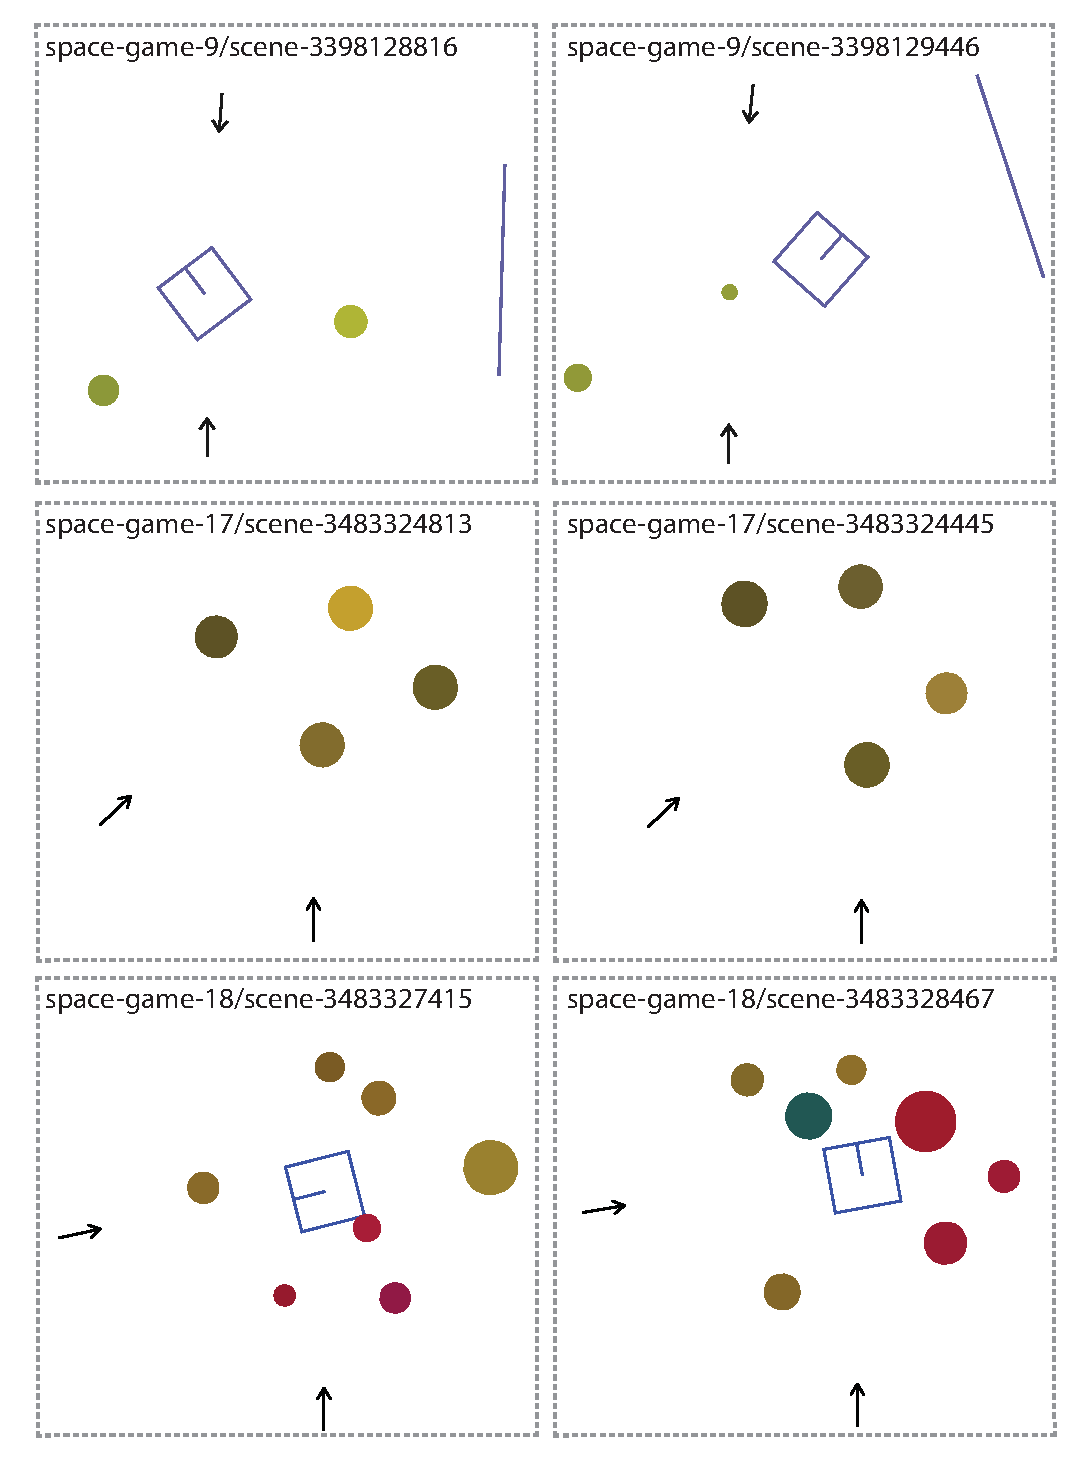
\includegraphics[width=0.8\columnwidth]{figs/spatial-scenes-overview-2}
\end{center}
\caption[Example scenes]{Example scenes from different 
spatial data sets. Each row shows 
scenes from a particular data set (the world model of 
robot \emph{a} is always shown). 
The first row shows a data set which features a global landmark 
(\emph{space-game-9}).
The middle row shows scenes of a data set without global landmark and
without box (\emph{space-game-17}). Lastly, a data set which features 
many objects is shown (\emph{space-game-18}).}
\label{f:spatial-scenes-2}
\end{figure}

\section{Social Mechanisms}
\label{s:social-mechanisms}\index{social mechanisms}
Language games require a number of social mechanisms to be in place. Joint attention, 
turn-taking behavior, pointing and other non-linguistic feedback these are mechanisms 
at the heart of the social interaction. Crucial social mechanisms required for these interaction 
are  considered prerequisites for studying the evolution of language. They constitute the 
background against which communication and evolution of communication takes place.

% joint attention
Joint attentional scenes \citep{tomasello1995joint}\index{Tomasello, M.} in which interlocutors 
are jointly attending to some object for some reasonable amount of time.
Establishing joint attention means in robotic experiments that two robots 
taking part in a language game must (1) share a physical environment, 
(2) attend to a set of objects in their surrounding, (3) track whether the 
respective other robot is able to attend to the same set of objects and 
(4) be able to manipulate attention by pointing to distal objects and perceiving
these pointing gestures  Joint attention is monitored by an external computer 
program, that has access to the world models of both interacting robots.  This system
initiates the interaction between two agents as soon as both agents
observe the same set of objects.  Spatial scenes are manipulated 
by a human experimenter to find spatial setups in which joint attention is
possible, the program monitors whether robots are seeing the same
set of objects and informs the experimenter whether the robots jointly attend 
to the same set of objects.

% turn taking
Social interactions have to be structured, so that agents can interpret the 
signals they exchange. For instance, if the hearer points before
he has received the utterance the speaker will have a hard time 
understanding the gesture. However, if the hearer points after
receiving the utterance, the speaker can assume that this is the response
to his speech act. Language games are coordinated by behavioral scripts. 
Every agent in the population knows the language game script and individually reacts
to changes in the environment and actions of the other robot. For
example the speaker triggers the action of pointing to the intended
topic when the hearer signals that he did not understand the
utterance. The scripts are implemented in the form of finite-state
machines: actions are performed depending on the current state in the
game flow, the perception of the environment and the history of the
interaction.

% non-linguistic feedback
In order to be able to learn and form spatial language systems, 
robots need non-linguistic means of conveying information, such as 
pointing to an object or conveying notions of success, failure and 
agreement in communication.  For demonstration purposes robots are
equipped with pointing gestures but in the communicative interactions 
underlying the results presented in this book, robots use a different 
mechanism in order to avoid further difficulties stemming from uncertainties in pointing (see
\citealp{steels1998stochasticity}\index{Steels, L.}\index{Kaplan, F.} for a discussion of the impact of
such uncertainties on the performance in language games). When a
robot wants to point to an object in the environment, he directly
transmits the coordinates of the intended object to the
interlocutor.  Since robots model object positions in their own
(egocentric) coordinate systems, additional steps have to be taken to
interpret these coordinates.  Most importantly the robot has to know
the position and orientation of the robot that is
pointing.  With this information robots transform the 
coordinates into their own coordinate system and interpret 
the pointing by choosing the closest object to the pointing 
coordinates in their world model. Similarly, robots directly exchange 
other non-linguistic feedback, for instance agreement and 
disagreement in communication by exchanging signals whose
meaning is shared. Moreover, linguistic utterances are directly passed between
interlocutors.



%
%\bibliographystyle{diss}
%\bibliography{papers,space}
%\end{document}


%\documentclass[a4paper,9pt,fleqn,notoc]{diss}
%% \renewcommand{\includegraphics}[1][1]{} 
%\begin{document}


\chapter{Embodied Cognitive Semantics with IRL}
\label{s:irl}
Artificial agents trying to achieve communicative goals in situated interactions
in the real-world need powerful computational systems for conceptualizing 
their environment. In order to provide 
embodied artificial systems with rich semantics reminiscent of human 
language complexity, agents need mechanisms for both conceptualizing complex 
compositional semantic structure\index{semantic structure}, but, also for 
actively reconstructing semantic 
structure in interpretation of ambiguous utterances.
Furthermore, the system must be open-ended and 
allow agents to adjust their semantic inventories in order to reach their goals. 
This chapter presents the computational system called
Incremental Recruitment Language (IRL)\index{Incremental Recruitment Language} 
that allows agents to represent and process complex conceptualizations\index{conceptualization}
of spatial scenes. The work presented here bases itself on substantial previous work. 
Key ideas of the IRL system have been laid out by \cite{steels2000emergence}\index{Steels, L.}, 
with progress reported in \cite{steels2005planning}\index{Steels, L.}\index{Bleys, J.}, \cite{vandenbroeck2008irl}\index{Van den Broeck, W.}, and
recently in \cite{spranger2010irl,spranger2012irl}\index{Loetzsch, M.}\index{Pauw, S.}\index{Spranger, M.}.

\section{Procedural Semantics}
\label{s:grounded-procedural-semantics}
\begin{figure}
\center
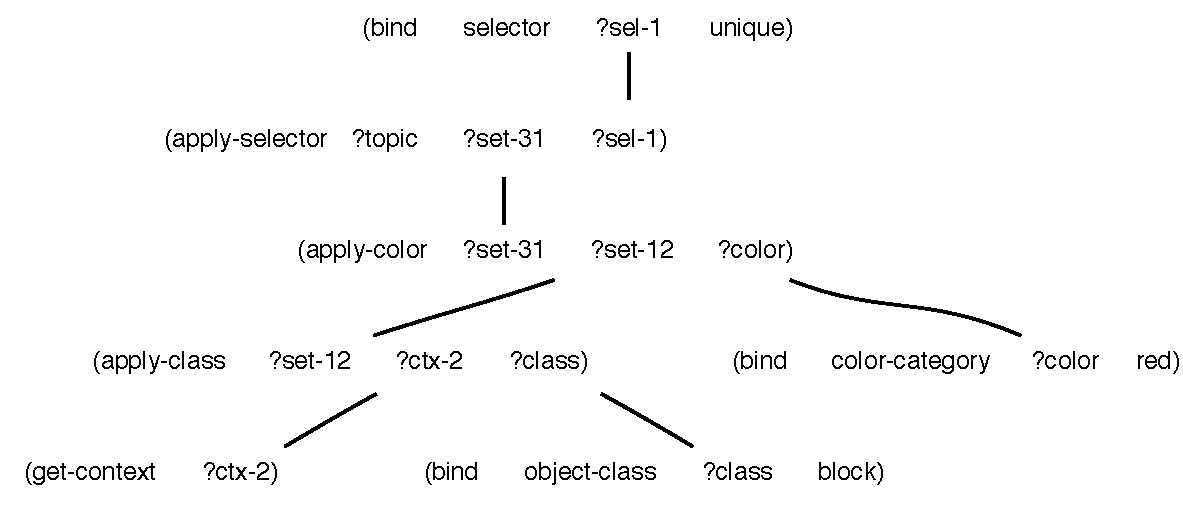
\includegraphics[width=1\columnwidth]{figs/the-red-block-network}
\caption{Semantic structure underlying the utterance ``der rote Block'' (the red block).}
\label{f:the-red-block-network}
\end{figure}

In order for a hearer to interpret an utterance, he has to apply the 
meaning conveyed in the linguistic structure to his perception of 
the context. Consequently, a speaker who 
uses language to achieve a certain communicative goal wants 
the hearer to execute a program \citep{johnson1977procedural}\index{Johnson-Laird, P. N.}, 
i.e. a set of operations that allow the hearer to, for example, discriminate 
an object in the environment or perform an action. Thus we model semantics, 
i.e. what it is a speaker wants the hearer to execute, as a 
program linking operations and data.  Let us start with an example. 
Suppose a speaker utters the phrase ``der rote Block'' (the red block) with the intention 
of making the hearer point to an object. In this case, the phrase 
encodes a program, i.e., set of operations, that are supposed to lead 
the hearer to identify the object in question. Presumably
the hearer of this utterance has to first filter the context for blocks, 
followed by the application of the color category
red, in order to arrive at the set of red blocks, which is used to 
compute the topic consisting of a single entity. A possible program, 
also called \emph{IRL-network}\index{IRL-network|see{semantic structure}}, is shown in Figure \ref{f:the-red-block-network}.
This network explicitly represents the chain of the four operations {\footnotesize\tt get-context},
{\footnotesize\tt apply-class}, {\footnotesize\tt apply-color} and {\footnotesize\tt apply-selector}
by linking their arguments through variables 
(starting with {\footnotesize\tt ?}). The network also 
includes the color category {\footnotesize\tt red}, 
the object class {\footnotesize\tt block} and the selector 
{\footnotesize\tt unique} which are introduced via so called 
\emph{bind statements}, as in 
{\footnotesize\tt (bind color-category ?color red)}. We collectively
refer to concepts, categories etc. as \emph{semantic entities}\index{semantic entity}.

IRL-networks consist of two types of nodes 
\begin{description}
\item[Cognitive operations,] also called \emph{semantic operations},\index{cognitive operation}
are the algorithms used in conceptualization. They encode a particular cognitive 
function such as categorization using a color category,
applying a selector or applying an object class and many more as will be shown
see later in this book for the domain of space. Cognitive operations 
are identified by their name, e.g. {\footnotesize\tt apply-color} and
they have a set of arguments which can be linked to other operations
or semantic entities via variables (starting with {\footnotesize\tt ?}).
\item[Semantic entites] is the general term for referring to prototypes,
concepts and categories that are used by cognitive operations.
Besides such long-term data, semantic entities can also be
discourse representations, the representation of the current context
and data exchanged between cognitive operations. They
are introduced explicitly in the network via {\footnotesize\tt bind}-statements
which are special operations for retrieving the actual data representation
using a pointer or shorthand notation for it. For instance, 
the statement {\footnotesize\tt (bind color-category ?color red)}
encodes the access to the color category {\footnotesize\tt red} which
is a prototype represented using values for different color channels.
\end{description}


\begin{figure}
\center
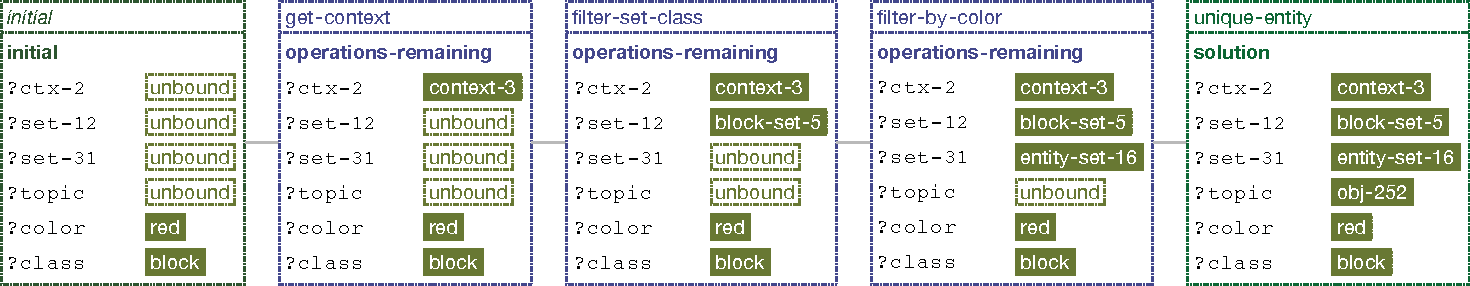
\includegraphics[width=1\columnwidth]{figs/evaluation-tree}
\caption[Evaluation of an IRL-network]{Progressive evaluation 
of the network in Figure \ref{f:the-red-block-network}
on the context shown in Figure \ref{f:scene}.
From left to right, each node represents a step in the evaluation process. From top to bottom, the evaluated operation, the node status, and the current list of bindings of each node are shown. A consistent solution with bindings for all variables is found in the last node, and the value 
{\footnotesize\tt obj-252} is indeed a unique red block (compare \ref{f:scene}).}
\label{f:evaluation-tree}
\end{figure}

\section{Evaluation}\index{cognitive operation!evaluation}
A program such as the one in Figure \ref{f:the-red-block-network} is \emph{evaluated}, 
by a speaker to test the semantic structure with respect to the 
particular communicative goal, or by a hearer in order to interpret an utterance.
Evaluation is a process which cycles over the network and progressively computes values
for variables, a process called \emph{binding}.
When the network in Figure \ref{f:the-red-block-network}
is evaluated the following happens. First {\footnotesize\tt get-context} gets the current 
world model from the perceptual processes that are monitoring the 
environment for events and objects and binds it to the variable 
{\footnotesize\tt ?ctx-2}. This is followed by the evaluation of the {\footnotesize\tt apply-class}
operation which computes a similarity score for how similar every object
in the context is with respect to the object class {\footnotesize\tt block}. 
This yields the set of objects from the context with each object 
scored using the computed similarity. The set is bound to the variable {\footnotesize\tt ?set-12}. 
Because this variable is linked to the operation {\footnotesize\tt apply-color}, 
the set bound to the variable {\footnotesize\tt ?set-12} is further processed using the 
color category {\footnotesize\tt red}. {\footnotesize\tt apply-color} first computes
a similarity score for every object in the input set to the color category 
{\footnotesize\tt red} which is multiplied with the similarity score the object
already has from the application of the class {\footnotesize\tt block}.
This yields a new set of objects with multiplied similarity scores.
The set is bound to the variable {\footnotesize\tt ?set-31}. Lastly, {\footnotesize\tt apply-selector} 
checks the objects in {\footnotesize\tt ?set-31}, finds the object with 
the highest similarity score and binds it to the variable {\footnotesize\tt ?topic}
which is the referent\footnote{Note that the word ``object'' here refers 
to an agent's private representation of 
things he has perceived in the world and only 
indirectly refers to the physical object which is the referent.
} of the phrase ``der rote Block'' (the red block).
Figure \ref{f:evaluation-tree} gives an idea how variables get progressively 
bound when the IRL-network is evaluated.

This is only one example how such a network can be evaluated. 
As has been argued in \cite{steels2000emergence}\index{Steels, L.},
language requires that semantic structure does not encode control flow, but rather 
data flows in all directions and is computed wherever possible.
For this, operations need to be able to function in different directions with
varying input-output parameters
For instance, the operation {\footnotesize\tt apply-class} which has three arguments, 
applies a class such as {\footnotesize\tt block} to an input set, when the 
class is explicitly represented in the network. But, in case
this class is not introduced via a bind statement in the network, the operation
can also provide this information effectively turning this argument
into an output argument. This \emph{multidirectionality}\index{cognitive operation!multidirectionality} of operations 
proves important for dealing with missing items, for instance due to partial parsing 
of an utterance, but it is also needed when constructing semantic structure.


\section{Conceptualization and Interpretation}\index{conceptualization}\index{interpretation}
\begin{figure}
\center
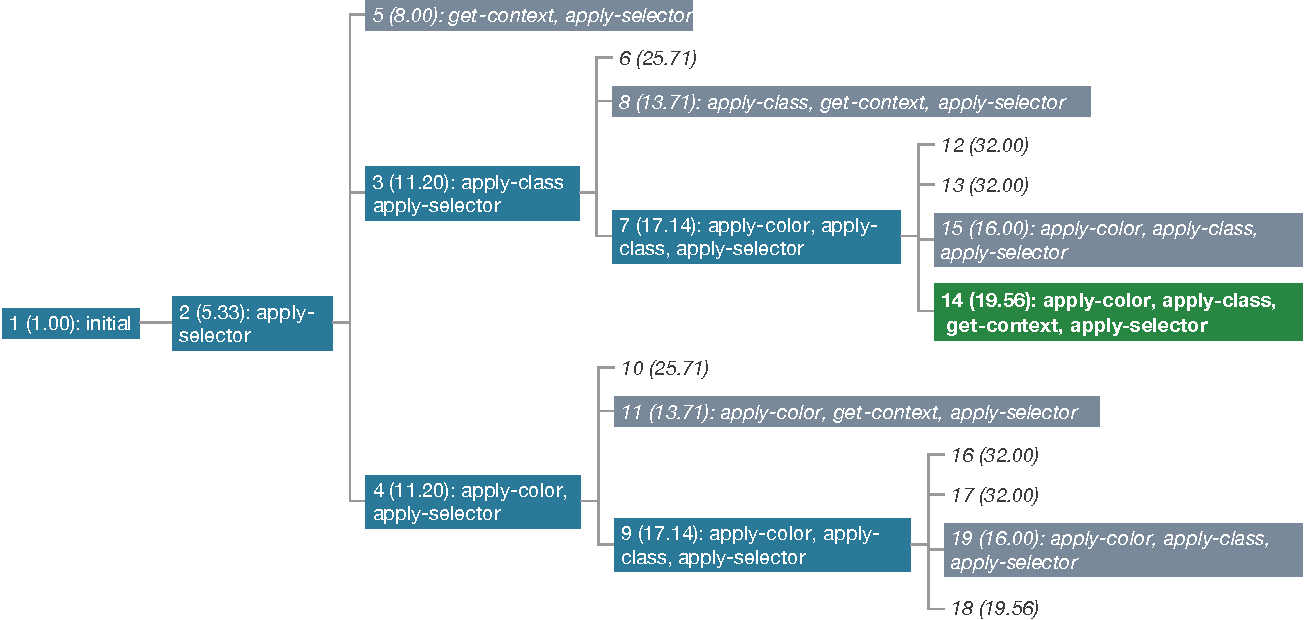
\includegraphics[width=1.0\columnwidth]{figs/composition}
\caption[IRL conceptualization search tree]{The search tree 
for finding the semantic structure seen in 
Figure \ref{f:the-red-block-network}. From left to right, nodes 
represent progressively growing programs combined from 
several chunks, which are each tried out and in some cases 
lead to solutions (green nodes).}
\label{f:the-red-block-search-tree}
\end{figure}

There are two scenarios in which agents autonomously compose semantic
structure like the one just described (Figure \ref{f:the-red-block-network}). 
First, speakers have a particular communicative goal and need to construct 
semantic structure, for instance, for singling out the particular topic the 
speaker wants to draw attention to.
This process is called \emph{conceptualization}. In the second scenario, 
hearers use information parsed from the observed utterance and their 
knowledge about the current context of the interaction to 
actively reconstruct meanings from the potentially partial 
structures parsed by the language system. We call this process 
\emph{interpretation}. Both cases are equally important and
they both conceive the process of building semantic structure as a heuristically
guided search process that explores the space of possible IRL-networks 
driven by the agent's particular communicative goal and the information
available to him.

In conceptualization, in other words while ``planning what to say'' 
\citep{steels2005planning}\index{Steels, L.}\index{Bleys, J.}, a speaker searches for an IRL-network 
that, when executed by the hearer, will reach a particular given 
communicative goal in a particular context.  IRL-networks 
are constructed by assembling basic building
blocks, in particular, cognitive operations packaged into chunks
into more and more complex semantic structures. 
Each assembled structure is immediately tested by evaluating it which assesses
its compatibility with the current communicative goal and the perceived context.
Figure \ref{f:the-red-block-search-tree} shows an example of such a search process 
that has produced the program in Figure \ref{f:the-red-block-network} for discriminating 
the red block in Figure \ref{f:scene}. 
The search process for `good' semantic structure is guided by 
many different heuristics, one being that the structure can be expressed using the
language system available to an agent. Others are more focused on the particular
character of the communicative goal. If the goal is to discriminate an object 
in the environment, then it is beneficial to use more discriminative categories, 
i.e. categories that enlarge the distance between the similarity of the topic and 
the similarity of all other objects in the context. 

Search is also applied when an agent perceiving an utterance  tries to 
interpret it. The semantic structure an agent 
parsed from an utterance is often incomplete and
semantic entities, cognitive operations and links can be
missing in the network. Interpretation is a flexible, active process
by which agents use search to add missing items to the network.
Networks are immediately evaluated to see if they find a referent for 
the parsed utterance. The search process is constrained by the partial 
meaning parsed from the utterance and
the kinds of semantic structures that are appropriate in the current context.
The same scoring mechanisms
as for conceptualization ensures that only structure that is 
discriminating for a particular object (implicitly assuming that the 
speaker constructs structure based on these principles) will be considered 
and the best of all possible results is chosen as the interpretation of an utterance. 

\section{Chunking}\index{chunking}
Search spaces quickly become intractable because the number of 
possibilities for composing semantic structures increases exponentially 
with the number of cognitive operations. A look at language
is helpful here. Grammar can be analyzed as a sophisticated
tool that highly structures human language in order to manage not only
the search space of possible syntactic structure \citep{steels2006dampen}\index{Steels, L.}\index{Wellens, P.} but
perhaps more importantly the vast space of possible conceptual
structures. Parts of meaning that are covered by a particular
part of language can be stored as a \emph{chunk} and 
then used as an basic atomic unit in composition.
Ready-made semantic structure dramatically reduces the search space. If a structure like
the final structure in Figure \ref{f:the-red-block-network} is
constructed from scratch using simple operations, the search tree
would have a search depth of three (essentially one step in depth per
operation). However, every time an operation is added to a program, it
can be linked to the current structure in multiple ways, which leads
to an explosion of nodes on every layer of depth. Hence, the system
soon has to deal with a wide search tree, where every node will be 
executed and tested against the context. Consequently, using chunking 
dramatically increases the performance of the system, even in simple examples.

Chunks have an important role in the study of language because
they package strategies for conceptualizing reality.
Chunks allow to research how cognitive operations
form strategies for conceptualizing reality, how these
strategies can be adapted by agents and how strategies
become conventionalized. For studying conventionalization, 
chunks have scores. This allows to track the success of each strategy with
respect to the communicative goals, e.g. discriminative power
of a strategy, but also with respect to communicative success. 
Strategies for conceptualizing reality are tightly linked to 
language. For instance, one can image that the
chunk in Figure \ref{f:the-red-block-chunk} which 
is extracted from the network in Figure \ref{f:the-red-block-network}
could be the semantics expressed by a determined adjective
noun phrase construction. One important claim is that the structure in language, 
in particular in grammar is tightly connected to the conceptualization
of reality underlying every utterance. So the fact that in English
noun phrases have determiners or, for instance, that in Russian all
verbs are marked for aspects suggests that these languages 
require speakers to conceptualize reality in a certain way and
mark these conceptualizations in language. 



\begin{figure}
\center
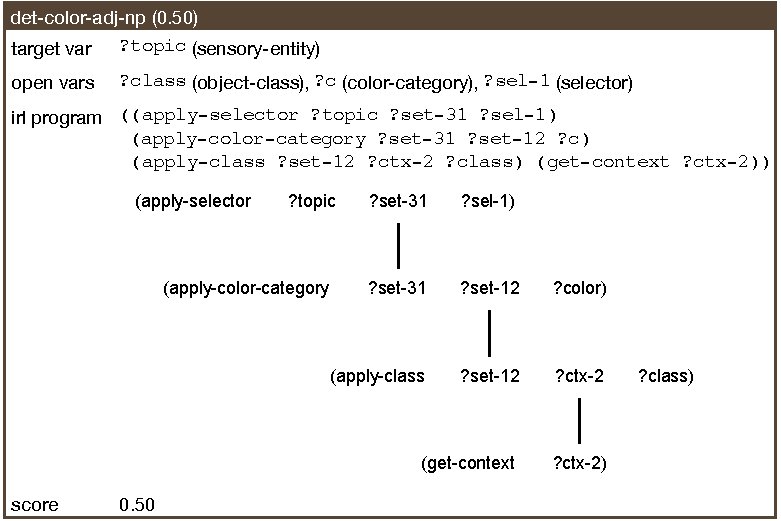
\includegraphics[width=1.0\columnwidth]{figs/det-color-adj-np-chunk}
\caption[Color-adjective noun phrase chunk]{Chunk representing the 
meaning of a determined color-adjective noun phrase. Chunks consist 
of an IRL-network, plus additional information used for processing: 
a target variable and open variables. These variables are typed 
(see brackets for type information)
and they are used in conceptualization and interpretation for combining chunks
to larger structures. The target variable of a chunk can be linked to the open
variable of another chunk. Which selector is used, 
which object class and which color category are is mostly
determined by evaluating the network which yields bindings for
the variables. Since the corresponding variables are open variables
the information can also be provided by other chunks or in interpretation
by the actual lexical items observed in the utterance. Chunks also have a score
which can reflect the degree to which they are conventional 
ways of conceptualizing reality.}
\label{f:the-red-block-chunk}
\end{figure}


\section{Grounding}\index{grounding}
Another important issue is grounding. 
There are now many proposals of how agents can ground lexicons and 
categorical systems in sensorimotor interaction with the environment 
\citep{billard1998grounding,vogt2001bootstrapping,steels2008grounding}\index{Billard, A.}\index{Steels, L.}\index{Dautenhahn, K.}\index{Vogt, P.} and 
IRL is designed to allow such 
insights to be applied straightforwardly. For instance, the 
implementation of the operation for {\footnotesize\texttt{apply-color}} is in part based on 
findings about how basic color categories can be grounded in the sensor 
data streams of digital cameras \citep{steels2005coordinating,bleys2009grounded}\index{Steels, L.}\index{Bleys, J.}\index{Spranger, M.}\index{Belpaeme, T.}\index{Loetzsch, M.}.
Similarly, other grounding mechanisms such as for events 
\citep{siskind2001grounding,steels2003events}\index{Siskind, J. M.}\index{Steels, L.}\index{Baillie, J.-C.} are easily instantiated in IRL operations. 

One of the main claims in this book is that agents co-evolve syntax 
and semantics. Chunks are one way in which agents can
shape strategies for conceptualizing reality. Another
is related to the semantic entities themselves and the fact that the
number of prototypes and categories and their particular 
representation is not fixed. For instance, there is now 
abundant research in the formation of basic color categories 
\citep{steels2005coordinating,belpaeme2007language}\index{Steels, L.}\index{Bleys, J.}\index{Belpaeme, T.}
and how agents can invent, adopt and shape their inventory
of color categories based on the environment they are
facing. These insights into adaptive categories,
but also names and individuals can be incorporated into
IRL which provides mechanisms for the creation and
adaptation of categories in semantic structure.


\section{Discussion}
IRL is a powerful system that for the first time allows 
to study complex semantic phenomena that go beyond
purely lexical studies. IRL is a general system for 
representing the procedural semantics
of utterances. It establishes a link between perception and
language by providing a mechanism for representing the meaning
of utterances, finding and interpreting the meaning of utterances.
Moreover, IRL is designed to allow language processing
to be a flexible, adaptive process which can be extended
by new cognitive operations, new chunks, and new categories 
at any moment. Moreover, IRL provides mechanisms for
tracking the success of semantic material such as 
chunks and categories. 


The oldest and in some sense most similar system 
to what I have presented here is Winograd's SHRDLU 
\citep{haddock1989computational,winograd1971procedures}\index{Haddock, N. J.}\index{Winograd, T.}, However, SHRDLU misses the key aspects of grounding, active interpretation and conceptualization 
as a search process. Other work such as \cite{bailey1997modeling}\index{Bailey, D.}\index{Narayanan, S.}\index{Feldman, J.}
and \cite{siskind2001grounding}\index{Siskind, J. M.} 
focus mostly on lexical meaning. Some approaches
have taken more general approaches e.g. to event structure \citep{narayanan1999moving}\index{Narayanan, S.} 
but stay mostly tied with that particular domain. One of the few approaches talking about 
objects and events in the same framework is \cite{roy2005semiotic}\index{Roy, D.}, which is comparable 
to ours, but so far has been a theoretical proposal only.


%\bibliographystyle{diss}
%\bibliography{papers,space} 
%\end{document}



%\documentclass[a4paper,9pt,fleqn,notoc]{diss}
%% \renewcommand{\includegraphics}[1][1]{} 
%\begin{document}

\chapter{Construction Grammar with FCG}
\label{s:fcg}
Construction Grammar posits that  linguistic
knowledge is organized in the form of ``constructions'' \citep{goldberg1995constructions,croft2001radical}\index{Goldberg, A.}\index{Croft, W.}
which are mappings of semantics and pragmatics to syntax, 
i.e. words and grammar, but also phonology, prosody or intonation. 
Typically, Construction grammarians take a functional view on language
and analyze every piece of language as a tool for communication and 
in terms of the syntactic and semantic function it performs.
The theoretical framework of Construction Grammar
is important for this book, because it integrates 
semantics with syntax and opens up 
ways for understanding the acquisition and evolution
of language as a tool for solving communicative problems 
in which all elements of processing from semantics to
syntax can be used as a tool for solving these
problems. 

Every part of an utterance has meaning and a semantic function. The 
meaning of a lexical item is the reference to the category, prototype 
or concept that it refers to. Its function is how it is used both 
in the semantic structure underlying the phrase  and in the
syntactic structure of the phrase. The following two examples
include the word \textit{rot} (`red') but they use the word in completely 
different syntactic and semantic structures.
\ea\label{ex:4:1}
der rote Block\\
\glt `the red block'\\
\z
\ea\label{ex:4:2}
Rot ist eine Farbe\\
\glt `red is a color'\\
\z
% \begin{enumerate}
% \item \textit{der rote Block} (`the red block')
% \item \textit{Rot ist eine Farbe} (`red is a color')
% \end{enumerate}
In Example \REF{ex:4:1} \textit{rot} (`red') is used to modify the set of objects
denoted by the word \textit{Block} (`block') whereas in \REF{ex:4:2} the
statement is about the color itself. We can precisely capture 
these differences in semantic function using cognitive operations
and IRL (an structure for Example \REF{ex:4:1} can be found in \sectref{s:irl}). 
The semantic function is coupled to a particular expression
in syntax. In Example \REF{ex:4:1} the color is expressed
as an adjective which signals its use as a modifier.  
In Example \REF{ex:4:2} the color is expressed as a noun and
signals that the subsequent verb phrase is a fact about the color itself. 
In production, the speaker can therefore choose to express
the category as an adjective if the category is linked to the corresponding
cognitive operation (e.g. {\footnotesize\tt apply-color}). In parsing, when
he observes a color adjective this allows him to infer
that he is supposed to modify a set of objects using that operation.
Which set of objects the color adjective modifies is determined
by the larger syntactic and semantic context. For instance, in Example
\REF{ex:4:1} the adjective is part of an adjective noun phrase that 
indicates which set is modified by the color category namely
the set of blocks. From the viewpoint of the adjective noun phrase
the adjective has the semantic function of providing a modifier and in 
particular of modifying the set of objects denoted by the noun. Of course, other adjectives,
such as spatial adjectives can have the same function within an 
adjective noun phrase. The modified set is then input to another
operation namely the operation {\footnotesize\tt apply-selector}
which is marked by the determiner. So what we can see already in 
these simple examples are mappings 
from semantics to syntax and back, where every aspect of syntax,
i.e. words and grammatical relations
have a specific effect on the semantic interpretation of the phrase.
Vice versa, the speaker can use all the potential of syntax to
communicate precise semantic distinctions that he wants to convey.
The key item for analysis is the function of items 
both in syntax and semantics. 
These dependencies between syntax and semantics can be easily
operationalized using FCG\index{Fluid Construction Grammar}
\citep{beule2005hierarchy,steels2005linking}\index{De Beule, J.}\index{Steels, L.}\index{Neubauer, N.}. 

Throughout this book language processing is implemented
in FCG, a computational implementation of Construction Grammar. FCG is (1) a formalism
that provides a notation for specifying constructions, (2) a
an engine that processes linguistic structure by applying constructions, 
in order, to produce utterances or parse meanings, and (3) a set of design principles
for organizing the grammar and linking grammar to 
representations of semantics, in particular, to semantic structure 
formalized using IRL. 

\section{Linguistic processing}
Linguistic processing encompasses both production and parsing
of utterances. In production, FCG starts from a conceptualized
meaning and tries to translate as much as possible of
the semantic structure conceptualized by IRL into syntactic structure, 
i.e. words and grammatical relations using constructions in the linguistic inventory. 
In parsing this process is reversed and the construction inventory is used
to recover as much semantic structure from an utterance as possible.
Processing is organized around the \textsc{transient structure}\index{transient structure}
which acts as a blackboard representing the current state of processing.
Constructions work like rules -- if a construction is applicable,
i.e. if conditions for its application are met, the construction
can change the transient structure.
Over time the transient structure accumulates information provided by the different constructions
that have applied until some end state is reached, for instance,
no construction can apply anymore.

\begin{figure}
\begin{center}
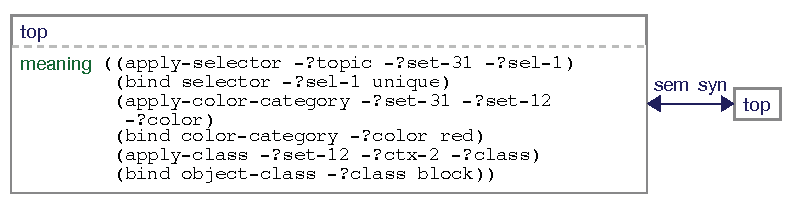
\includegraphics[width=.8\textwidth]{figs/simple-grammar-initial}
\end{center}
\caption[Initial transient structure]{\index{transient structure!initial}Initial transient structure which 
contains only the meaning 
to be expressed in the top-unit of the semantic pole (left).
There is no hierarchy yet and the syntactic pole (right) is empty.}
\label{f:initial-structure}
\end{figure}

\begin{sidewaysfigure}
\begin{center}
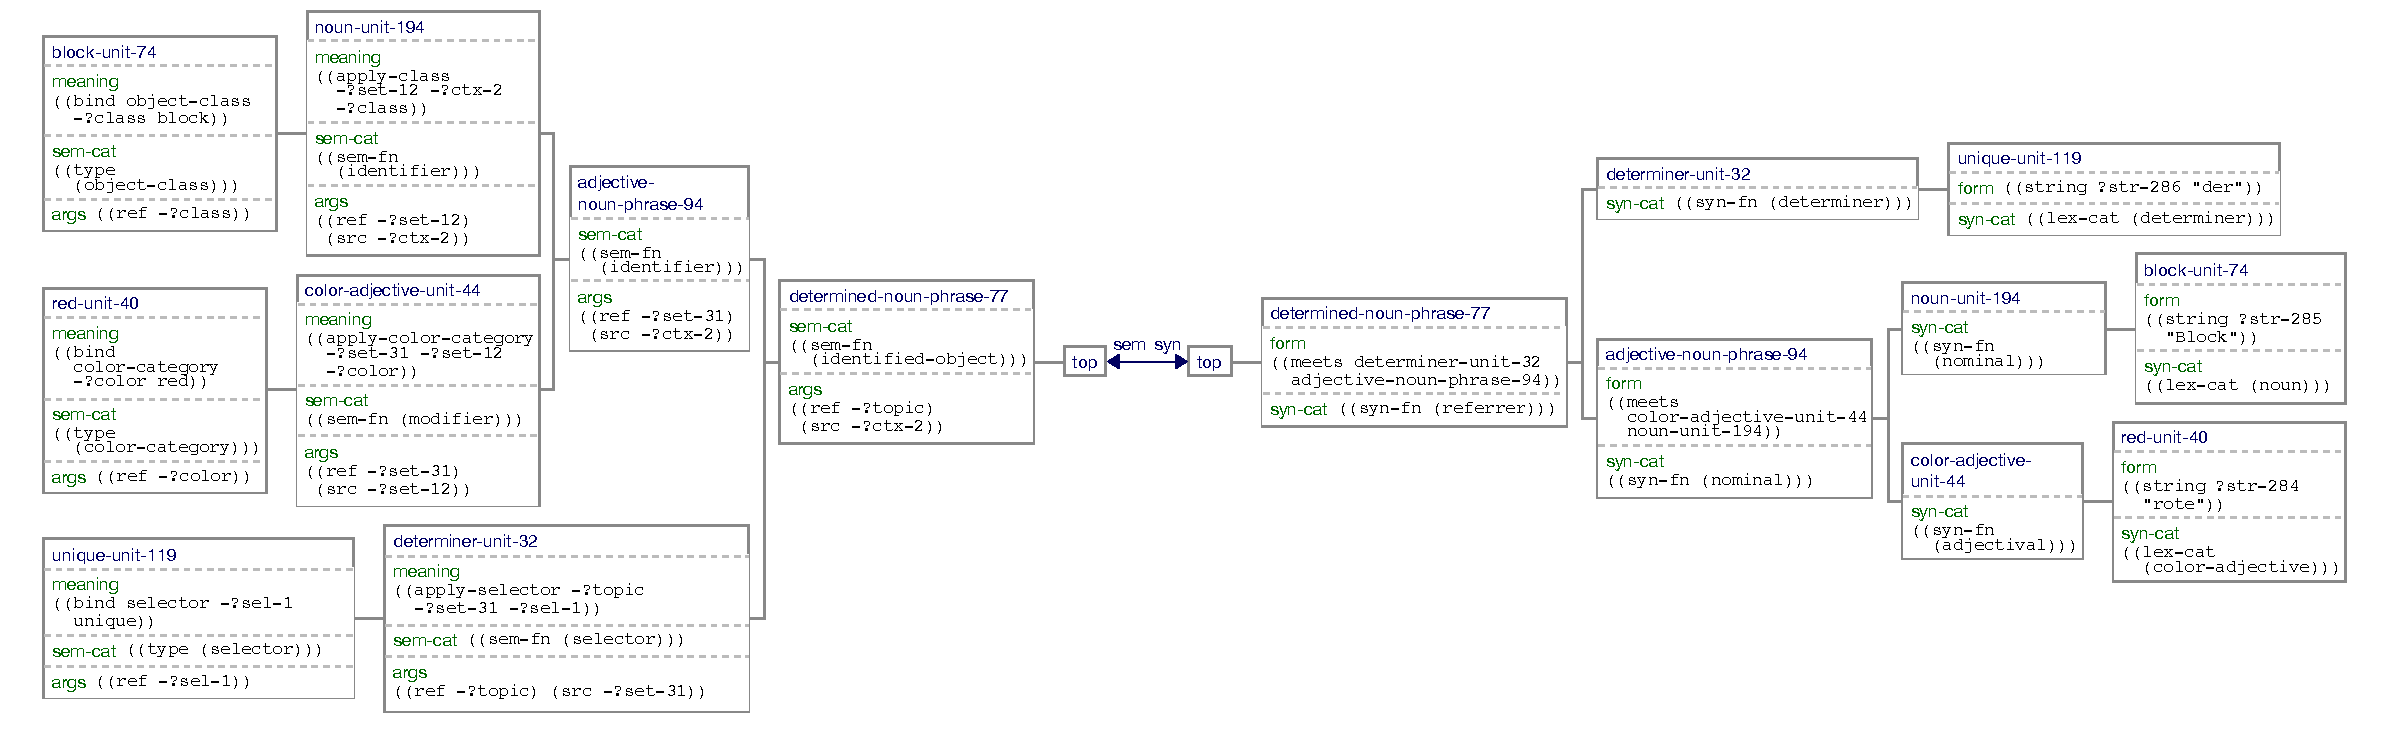
\includegraphics[width=\textwidth]{figs/simple-grammar-final}
\end{center}
\caption[Final transient structure]{\index{transient structure!final}Final transient structure after 
many constructions of a simplified German grammar have been applied.
The structure consists of units which are hierarchically organized starting
from the top-unit. The meaning to be expressed is distributed over various 
units on the semantic side. Units feature 
semantic and syntactic categorization ({\footnotesize\tt sem-cat} and {\footnotesize\tt syn-cat})
which was build up in processing to organize constituent structure and
allow for high-level constructions to abstract from individual items.
On the syntactic side units have {\footnotesize\tt form} features consisting
of strings providing words and, so called ``meets constraints'' which introduce 
word order.}
\label{f:final-structure}
\end{sidewaysfigure}

\subsection{Transient structure}\index{transient structure}
The transient structure\index{transient structure} has two poles: a semantic and a syntactic pole.
Information regarding meaning is accumulated on the semantic
side, information about words and grammatical relations are
gathered on the syntactic side. Information is organized into 
units identified by a {\footnotesize\tt unit-name}. Units consist of {\footnotesize\tt attribute-value} pairs. 
In order to represent constituent structure, units can form hierarchies 
in which some units are hierarchically linked to other units effectively 
building tree like structures.
In the beginning of processing the transient structure\index{transient structure} is filled with 
information either from the conceptualization 
processes, e.g. in production, or from the utterance observed, e.g.
in parsing. Subsequently, constructions change the transient structure by adding new
units, introducing hierarchy, changing the value of attributes or by introducing 
new attributes. Figures \ref{f:initial-structure} and \ref{f:final-structure} show the transition from 
an initial transient structure\index{transient structure} which only contains a single unit, called ``top-unit'' 
on each side to a final transient structure with hierarchical organization of units 
and many more features. The initial structure only contains a 
meaning on the semantic side. The final structure contains,
among other things, strings and syntactic word order constraints 
which can be used to build an utterance, a process called \textsc{rendering}.
Figures~\ref{f:initial-structure} and \ref{f:final-structure} show graphical representations
of the list representation (s-expression) used in processing. The
following restates the initial transient structure\index{transient structure} as s-expression.
% \begin{footnotesize}
\begin{lstlisting}
((top
  (meaning ((apply-selector -?topic -?set-31 -?sel-1)
            (bind selector -?sel-1 unique)
            (apply-color-category -?set-31 -?set-12 -?color)
            (bind color-category -?color red)
            (apply-class -?set-12 -?ctx-2 -?class)
            (bind object-class -?class block)))))
<-->
((top))
\end{lstlisting}
% \end{footnotesize}
The top shows the semantic pole. The bottom, after the {\footnotesize\tt <-->},
shows the syntactic pole. Both poles have one unit (the top-unit). 
On the semantic side the top-unit has one attribute, the meaning attribute
which has an IRL-network in list form as its value. 
The following shows the final structure in the same representational 
format.
% \begin{footnotesize}
\begin{lstlisting}
(...
 (color-adjective-unit-44
  (meaning ((apply-color-category -?set-31 -?set-12 -?color)))
  (sem-subunits (red-unit-40))
  (sem-cat ((sem-fn (modifier))))
  (args ((ref -?set-31) (src -?set-12))))
 (red-unit-40
  (meaning ((bind color-category -?color red)))
  (sem-cat ((type (color-category))))
  (args ((ref -?color))))
  ...
 (top (sem-subunits (determined-noun-phrase-77))))
<-->
(...
 (color-adjective-unit-44
  (syn-subunits (red-unit-40))
  (syn-cat ((syn-fn (adjectival)))))
 (red-unit-40
  (form ((string ?str-284 "rote")))
  (syn-cat ((lex-cat (color-adjective)))))
  ...
 (top (syn-subunits (determined-noun-phrase-77))))
\end{lstlisting}
% \end{footnotesize}
Only parts of the complete final structure are shown,
in particular, three units on each pole are shown the 
{\footnotesize\tt red-unit-40}, {\footnotesize\tt color-adjective-unit-44}
and {\footnotesize\tt top}. In contrast to the initial transient structure,
meaning is distributed across different units.
Notice that which unit is subunit of another is coded by a special
attribute called {\footnotesize\tt syn-subunits} on the syntactic pole
and {\footnotesize\tt sem-subunits} on the semantic pole. Compare
this with \figref{f:after-red-cxn} which shows the hierarchy in the final 
structure. For example {\footnotesize\tt red-unit-40} is a subunit of 
{\footnotesize\tt color-adjective-unit-44}.

\begin{figure}
\begin{center}
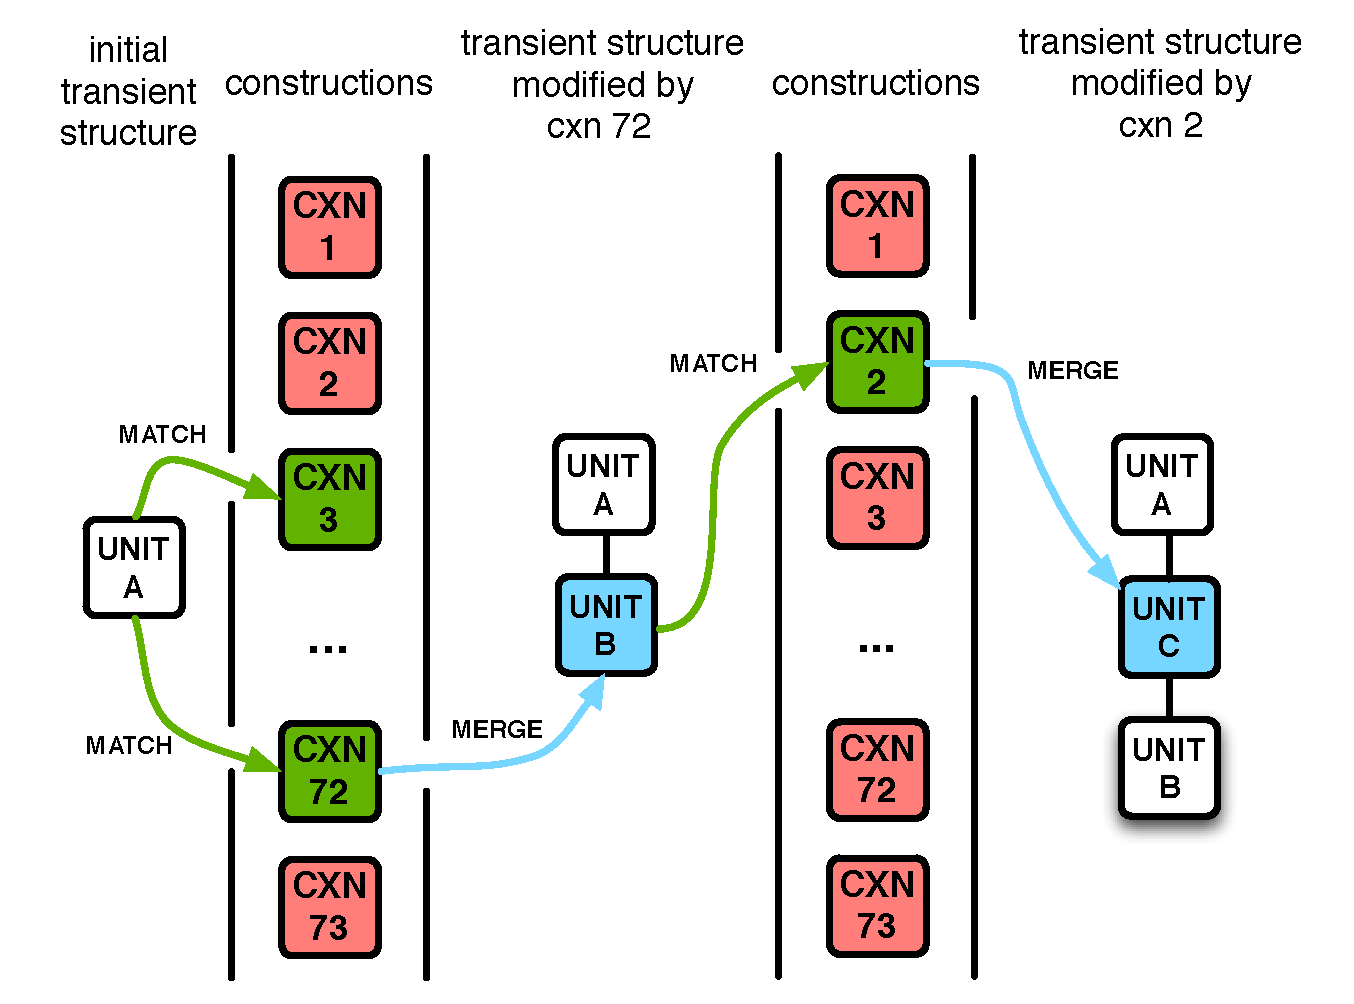
\includegraphics[width=0.75\textwidth]{figs/high-level-cxn-application}
\end{center}
\caption[Construction application]{This figure shows a schematic view on 
construction application (Figure adapted from \citealp{steels2011design}\index{Steels, L.}).
Starting from the initial transient structure\index{transient structure} (left)
all constructions in the set of constructions are tested whether they 
match with the structure. Two constructions match with the
initial transient structure. If a construction matches it 
can merge new information. Construction 72 adds 
unit C. After the structure has been changed, the process continues
and all constructions are checked whether they merge with
the transient structure\index{transient structure} modified by construction 72.
Because construction 72 has applied, the transient
structure is in a state such that construction 2 can now apply. 
This was previously not the case. Construction 2 is depending on
information provided by construction 72. Subsequently, construction 2 
further changes the transient structure and so on and so forth.
Often multiple constructions from the set of constructions can apply.
For example, construction 3 could also change the initial transient structure\index{transient structure}.
This poses a general problem in processing which is solved
by using a search algorithm described later in this section.}
\label{f:cxn-application}
\end{figure}

\subsection{Constructions}\index{construction}
Constructions are organized in the same way as transient structures\index{transient structure}.
They consist of two poles and the data in each pole are organized in terms of units, 
attributes and values. FCG supports bi-directional constructions which means
that the same construction is used in production and parsing. 
The difference between production and parsing is how the syntactic and semantic 
pole of a construction is used in each case. 
In production the semantic pole is used to check the applicability
of the construction. In parsing the syntactic pole is used. Applicability
of a construction is checked using a mechanism called \textsc{matching}.\index{matching}
Matching is based on the well studied concept of \textsc{unification} which \index{unification}
is a computational process for equating two terms in this 
case the semantic or syntactic pole of the construction with the corresponding 
pole of the transient structure. If matching succeeds, the construction can
change both poles of the transient structure\index{transient structure}, a process called \textsc{merge},
because it fuses information.
The precise inner workings of these two fundamental operations 
are described in \citet{steels2006fcg}\index{Steels, L.}\index{De Beule, J.}.
The most important fact is that matching in FCG mainly relies on 
variables, which in FCG (and in IRL) start with {\footnotesize\tt ?}.
In computational terms constructions specify (1) under which conditions
they apply and (2) if they apply how the structure should be changed.

\begin{figure}
\begin{center}
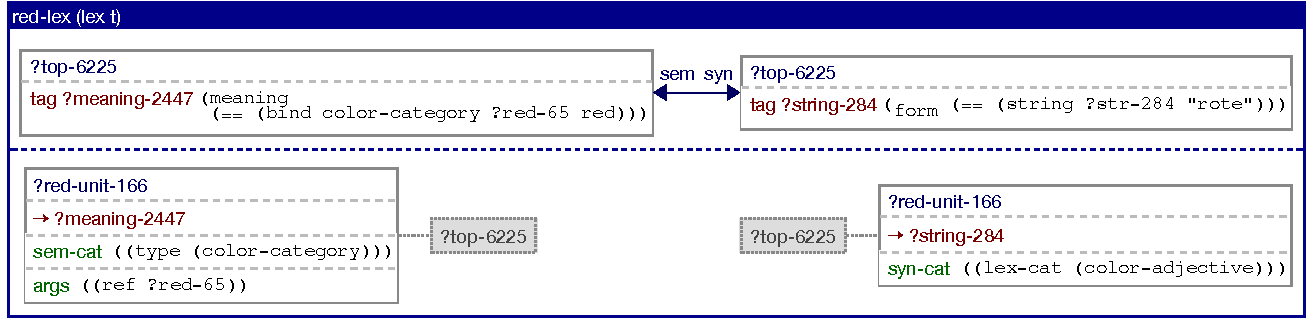
\includegraphics[width=\textwidth]{figs/lex-rot-cxn}
\end{center}
\caption[Schematic representation of a construction]{Schematic representation 
of a construction. The two poles
of the construction are shown. The top shows 
the tagged and matching parts of the construction. The 
bottom shows the hierarchy building part of the construction.}
\label{f:lex-rot-cxn}
\end{figure}

\figref{f:lex-rot-cxn} shows an example of a lexical construction that maps 
the color category {\footnotesize\tt red} onto the string \textit{rote} (`red')
(\figref{f:after-red-cxn} shows what happens
when this construction is applied to the initial transient structure\index{transient structure!initial}). 
The following shows the low-level list representation of the construction
schematically depicted in \figref{f:lex-rot-cxn}
% \begin{example}
\ea\label{e:red-lex-list}
% \begin{footnotesize}
% \begin{verbatim}[commandchars=\\\{\}]
\begin{lstlisting} 
((?top-6143
  (tag ?meaning-2381 
   (meaning (== (bind color-category ?red-57 red)))))
 ((j ?red-unit-158 ?top-6143)
  ?meaning-2381
  (sem-cat ((type (color-category))))
  (args ((ref ?red-57)))))
<-->
((?top-6143
  (tag ?string-251 (form (== (string ?str-251 "rote")))))
 ((j ?red-unit-158 ?top-6143)
  ?string-251
  (syn-cat ((lex-cat (color-adjective))))))
\end{lstlisting}\z
% \end{footnotesize}
% \end{example}
The top displays the semantic pole followed by the syntactic pole after the 
{\footnotesize\tt <-->}. In production the construction requires\index{production}
the meaning {\footnotesize\tt (bind color-category ?red red)} to be present.
If this is the case, the construction merges the information 
on the syntactic side, in particular the stem, into the transient structure\index{transient structure}.
Additionally, this construction builds hierarchy. It introduces a new unit
which is a subunit of the top-unit and which is used to collect
information for this particular lexical item. Already this simple 
construction uses the four basic ways in which constructions
interact with the transient structure\index{transient structure}:

\begin{description}
\item[Variables and matching] Constructions inevitably contain
many variables. Already the unit names in the transient structure\index{transient structure}
are changing every time a new utterance is parsed or a new meaning
is produced. But also, just to give another example, variables in the meaning 
linking cognitive operations are different every time IRL conceptualizes. 
Using a variable in one part of the construction and repeating it in another 
can lead to changes in the transient structure triggered
by matching and merging \citep{steels2006fcg}\index{Steels, L.}\index{De Beule, J.}.
Example \REF{e:red-lex-list}, for instance, uses matching and merging
by re-using the variable in the meaning {\footnotesize\tt ?red-57}
in the {\footnotesize\tt args} attribute. Whatever this variable binds
to in processing the re-occurring variable will make sure
that the data is available in both places.
\item[Hierarchy] Hierarchy is built using a special
operator called the ``J-operator'', which changes the
transient structure to include a new unit \citep{beule2005hierarchy}\index{De Beule, J.}\index{Steels, L.}.
The new unit can have units that are already present in the 
transient structure as children. A construction can therefore 
easily change the hierarchical structure of the complete pole.
The J-operator syntax is:
%\begin{example*}
\ea\label{e:j-op-syntax}
% \begin{footnotesize}
% \begin{Verbatim}[commandchars=\\\{\}]
\begin{lstlisting}
((J ?new-unit ?parent (?child-1 .. ?child-n))
 (new-attribute new-attribute-value))
\end{lstlisting}\z
% \end{Verbatim}
% \end{footnotesize}
%\end{example*}
In the example construction the J-operator is used on the semantic
and on the syntactic side. It introduces new units on both sides 
and adds information to this unit (in \figref{f:lex-rot-cxn}
the parts pertaining to the J-operator are shown below the dotted
line). Notice that the name of the new units is equal.
\item[Movement] Constructions can \emph{tag} attributes and
their values in order to move them around. In this example
construction, the tag-operator moves the bind statement pertaining to the
color category from the top-unit to the newly created unit.
The tag operator takes the following form:
% \begin{footnotesize}
% \begin{Verbatim}[commandchars=\\\{\}]
\begin{lstlisting}
(?unit (tag ?tag-variable (attribute attribute-value))
\end{lstlisting}
% \end{Verbatim}
% \end{footnotesize}
The operator binds whatever follows the variable {\footnotesize\tt ?tag-variable}
to the variable. If the variable is used in a J-unit, i.e. a unit with a J-operator, 
in another part of the construction, this denotes the place where 
{\footnotesize\tt (attribute attribute-value)} will be moved. The example
construction has {\footnotesize\tt tag} operators on the semantic side for moving the
bind statement to the new semantic unit. Similarly, on the syntactic side the
operator is used to move the string \textit{rote} to the new syntactic unit.
\end{description}

\begin{figure}
\begin{center}
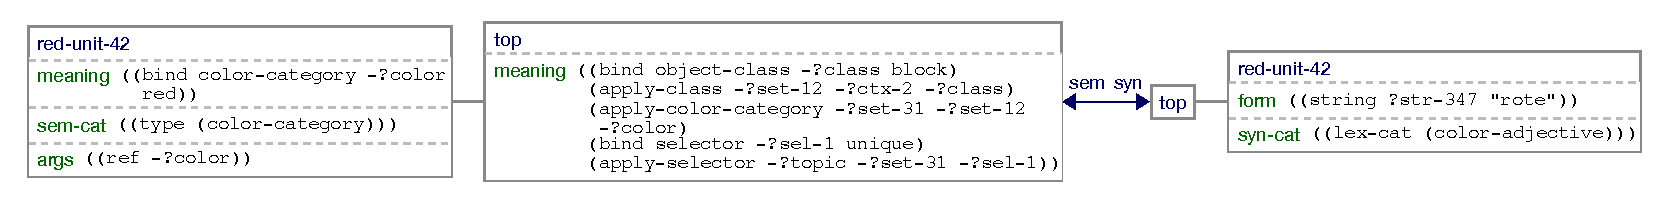
\includegraphics[width=\textwidth]{figs/simple-grammar-after-red-application}
\end{center}
\caption[Transient structure after lexical constructions applied]{%
Transient structure after the lexical construction applied. The construction
has introduced two new units using the J-operator. 
One on the semantic side and one on the syntactic side.
Both units have the same name {\footnotesize\tt red-unit-42}. The construction introduced
the string \textit{rote} on the syntactic side and the bind statements used for 
triggering the construction has been moved moved using the tag-operator 
from the top-unit to the new semantic subunit.
The construction also added new semantic and syntactic categories
({\footnotesize\tt sem-cat} and {\footnotesize\tt syn-cat}) that can be used by 
subsequent constructions.}
\label{f:after-red-cxn}
\end{figure}

\subsection{Search}
Constructions are organized in a pool of constructions. In principle, constructions compete for access 
to the transient structure in processing. More than one construction 
can typically apply to the transient structure and the question is how to organize
the process if there are multiple constructions that want to change
the transient structure. In the absence of a~priori rules to 
prefer one construction over another, each construction that can 
apply to the transient structure\index{transient structure}, is tried in a different branch of a 
heuristically guided search process. In other words, instead
of having competing constructions change the same transient
structure, the structure is copied and each potentially
applying construction is applied to a copy without necessarily 
influencing the other. Naturally, this leads to different
branches in processing, in which each branch
computes a particular parsing or production result.
Search is represented using a search tree in which each
node contains a transient structure. The initial node 
contains the initial transient structure. Leaf nodes contain final structures.
The search process itself can be manipulated. 
For instance, it is possible to remove and refrain from processing 
duplicate nodes which contain the same transient structure\index{transient structure}
and the order of following a particular branch can be 
influenced by how successful one predicts the branch to be.
\figref{f:fcg-search} shows an example search tree for 
production of the utterance \textit{der rote Block}.

\begin{figure}
\begin{center}

\includegraphics[width=1.0\columnwidth]{figs/der-rote-block-fcg-search}
\end{center}
\caption[FCG search tree in production]{FCG search tree which 
produces \textit{der rote Block} given the IRL-network
shown in \figref{f:the-red-block-network}.}
\label{f:fcg-search}
\end{figure}

\subsection{Design layer}
In order to design grammars it has proven beneficial
to abstract from the low level processing layer of FCG and 
add a representational layer that connects high level linguistic 
analysis with the processing engine of FCG.
The idea is to allow re-occurring problems in grammar design
to be solved using \textsc{templates} -- without having
to resort and copy the code needed for describing a construction
in the basic list notation. Templates 
are a general mechanism for expressing \textsc{design patterns}\index{design pattern},
i.e. solutions that can be re-used to deal with the
same problem occurring in different situations. For instance,
all grammars implement phrasal constructions. One 
of the main semantic functions of phrasal constructions 
is to introduce variable equalities for linking constituents.
A template encapsulates the solution to the problem 
of linking constituents in a way that the solution can be re-used in other
phrasal constructions of the same grammar, but ideally also for phrasal constructions in other grammars.
Templates are defined similar to functions. They
have a name and a set of arguments which are specific
to the template.
% \begin{example}
\ea\label{e:template-syntax}
% \begin{footnotesize}
% \begin{Verbatim}[commandchars=\\\{\}]
\begin{lstlisting}
(\emph{template-name} \emph{construction-name}
 \emph{:argument-1} \emph{value-1}
 \emph{:argument-2} \emph{value-2}
 ...
 \emph{:argument-n} \emph{value-n})
\end{lstlisting}\z
% \end{footnotesize}
% \end{example}

Let us consider an example. I redefine the lexical construction introduced earlier,
using a template called 
{\footnotesize\tt def-lex-skeleton}.
% \begin{example}
\ea\label{e:def-lex-rot}
% \begin{footnotesize}
% \begin{Verbatim}[commandchars=\\\{\}]
\begin{lstlisting}
(def-lex-skeleton red-cxn 
 :meaning (== (bind color-category ?cat red)) 
 :args ((ref ?cat))
 :string "rote")
\end{lstlisting}\z
% \end{Verbatim}
% \end{footnotesize}
% \end{example}
If this template is executed it translates into the 
low-level list representation in \REF{e:red-lex-list}. 

\section{Open-ended language evolution with FCG}
Besides the obvious requirement of computational
formalism for linguistic processing for computational
experiments, FCG has a number
of features that make it an optimal choice for studies
in language evolution. FCG is not fixed to a certain
set of constructions, a particular grammar layout, 
a particular set of meanings,
or even a particular set of semantic and syntactic 
categories. FCG solely provides 
dedicated mechanisms for processing language but
makes no actual claims about how a particular
phenomenon should be processed in language. 
% Most importantly it makes no claims about the 
% layout of the constructions designed to process
% a particular phenomenon. 
This allows different 
solutions to be explored by grammar designers.
But, most importantly, it allows artificial agents
to invent different constructions for solving a particular
problem in communication, track their success and
adapt them until the agents have conventionalized
a solution to their particular problem. 
% This is a point
% of utmost importance. 
Language is not a fixed system, but
rather a system negotiated by its users to reach
communicative goals in a decentralized manner. 
The fact that there are different solutions to solving
the same problem therefore requires formalisms
that are designed to be open to change syntactic and 
semantic categorization, and evolve meaning
structure and new constructions. FCG is such a formalism.

From a computational perspective, FCG provides
an easily manipulatable data representation, which makes 
inventing new constructions, changing and
adapting semantic and syntactic categories, and
introducing hierarchy or movement of data relatively easy.
As in Construction Grammar the \emph{unified} nature
of representation is important. There is absolutely
no difference in terms of representation and processing 
between lexical, functional or phrasal constructions. Hence, FCG
supports research into how constructions can change 
from lexical to grammatical constructions, which is 
of interest for the study of the influence of the grammaticalization 
processes on language evolution \citep{traugott1991grammaticalization}\index{Heine, B.}\index{Traugott, E. C.}.

Another important argument for the use of FCG is its robust
behavior in parsing and production. The search process\index{parsing}
for construction application and the bi-directional 
nature of constructions allow agents to produce
as much of the meaning as they can when they
are speaker. In parsing, the same process
allows agents to  recover as much of the semantics 
of a phrase as they possibly can. This is a prerequisite 
for any kind of grounded language learning let alone
language evolution. Agents have to get as much
information as possible from the different systems,
such as perception and conceptualization, but also
language processing. If agents would have to deal with
a grammar engine that essentially gives up on processing
as soon as an agent encounters a phrase that he
thinks is unconventional, learning the new unconventional
phrase can never occur or is significantly hindered. Whereas
if the grammar engine provides as much information as 
possible, agents have a much better shot at guessing
underlying meaning and making sense
of what was conveyed to them. Subsequently,
they can better represent the new parts of an 
utterance versus parts they already know.
Modeling this whole process as a search
process is an immense advantage of FCG.
Agents can track what changes when they
apply other constructions and explore different
possible parse and produce results, in order
to identify problems in language processing.

The last point with respect to the advantage of
keeping information from the search process that
governs linguistic processing is important, in particular
for the main problem studied in this book: conventionalization.
In order for agents to realize that constructions are competing
for the same string, the same grammatical structure or
the same meaning, it is vital to fully explore the search process.
If there are multiple ways of producing an utterance for a meaning,
for instance because there are multiple words to express
the same category, then the search can recover 
all of them. Together with a mechanism for tracking
success of constructions, the search can choose
the best one of them. After the interaction the agent can
then update the constructions used and those that
he could have used, for instance, by rewarding
successfully used constructions and punishing 
unsuccessful or unused constructions.
Constructions are equipped with a score that
allows agents to update their inventories
by scoring constructions according to their success
in communication. If scores get too low agents can remove
the affected constructions.

\section{Discussion}
There is no question that this is a short, in many ways too short,
introduction to FCG. FCG has been under continuous development
since 1998 and it has developed into a mature system which allows 
to research complex language phenomena such as Russian aspect 
\citep{gerasymova2010acquisition,gerasymova2012temporal}\index{Gerasymova, K.}\index{Spranger, M.}. The complexity of natural 
language has without doubt left its mark on the system and many design 
choices in the system are not immediately obvious,
unless one takes the scope of the research program into account.
Recently several book projects \citep{steels2011design,steels2012computational}\index{Steels, L.}
attempted to communicate the full scope of FCG research
performed in the last decade. The interested reader is referred
to these efforts to get a broader introduction.

%\bibliographystyle{diss}
%\bibliography{papers,space} 
%\end{document}

%% 4-6 The German Language System 
 \part{Reconstructing German locative phrases} 
 \label{p:german-locative-phrases}
 %\documentclass[a4paper,9pt,fleqn,notoc]{diss}
%\renewcommand{\includegraphics}[1][1]{} 

%\begin{document}

%%%%%%%%%%%%%%%%%%%%%%%%%%%%%%%%%%%%
\chapter{German locative phrases -- an introduction}
\label{s:german-spatial-language-introduction}
%syntactic distinctions mirror semantic distinctions\\
%vast space of semantic distinctions or spatial conceptualizations\\
%vast space of possible syntactic expression of spatial conceptualzations\\

To appreciate the complexity of spatial language one just needs
to consider a particular human language such as German.
The following chapters detail an elaborate reconstruction 
effort which targets locative German phrases (parts of this reconstruction
effort have been published in \citealt{spranger2011german}\index{Loetzsch, M.}\index{Spranger, M.}). 
I specifically focus on the processing of German locative phrases 
in a whole systems approach encompassing the perception, conceptualization,
as well as production and parsing of spatial phrases.
Before we jump to the implementation and the specific
challenges in modeling such a complex phenomenon, this introduction
overviews German spatial relations and highlights the syntax and 
semantics of German locative phrases, as well as the
close interaction of syntax and semantics. 
The claim is that important aspects of the syntactic structure of an utterance, i.e. 
the lexical items and the grammatical relations between them, work together to convey 
semantic structure, i.e. meaning. Vice versa, the varied syntactic 
devices in German spatial language allow to express subtle differences
in the conceptualization of spatial scenes. The German spatial language system serves 
as a beautiful example of how syntax connects to the extraordinarily rich world of 
spatial semantics. %The following paragraphs give a quick introduction to 
%German locative expressions. % We know this already.

%%%%%%%%%%%%%%%%%%%%%%%%%%%%%%%%%%%%

%\paragraph*{Spatial Relations}
% projective, topological
The literature distinguishes several classes of spatial relations 
available in German. Among them are projective, proximal and absolute relations
(see \figref{f:spatial-relations-taxonomy}).
\begin{description}
\item[Projective relations]\is{spatial relation!projective}-- sometimes also called \textsc{dimensional terms} 
\citep{eschenbach2004functional,herskovits1986language}\index{Eschenbach, C.}\index{Herskovits, A.} --  
in German comprise the class of six items referring to spatial dimensions
\textit{vor} (`front'), hinter (`behind'), \textit{\"uber} (`above'), \textit{unter} (`below'), \textit{rechts} (`right'), 
\textit{links} (`left') \citep{tenbrink2007space,tenbrink2005localising,wunderlich1991lokale}\index{Herweg, M.}\index{Tenbrink, T.}\index{Wunderlich, D.}. 
Traditionally, and for reasons of distinct syntax and semantics the
class of projective relations is further divided into \textsc{frontal} (\textit{vor} 
and \textit{hinter}), \textsc{lateral} (\textit{links} and \textit{rechts}), 
\textsc{horizontal} (comprising lateral and frontal relations), and 
\textsc{vertical relations} (\textit{\"uber} and \textit{unter}). 
\item[Proximal relations] are part of the larger class of topological relations\is{spatial relation!proximal}
that structure space with respect to proximity, contact and inclusion 
\citep{Grabowski1996prepositional}\index{Weiss, P.}\index{Grabowski, J.}. For this book proximal relationships
such as \textit{nah} (`near') and \textit{fern} (`far') are important.
\item[Absolute relations] refer to cardinal directions,\is{spatial relation!absolute}
for instance \textit{n\"ordlich} (`north'), \textit{westlich} (`west'), \textit{\"ostlich} (`east') and
\textit{s\"udlich} (`south').
\end{description}

\begin{sidewaysfigure}
%\begin{figure}
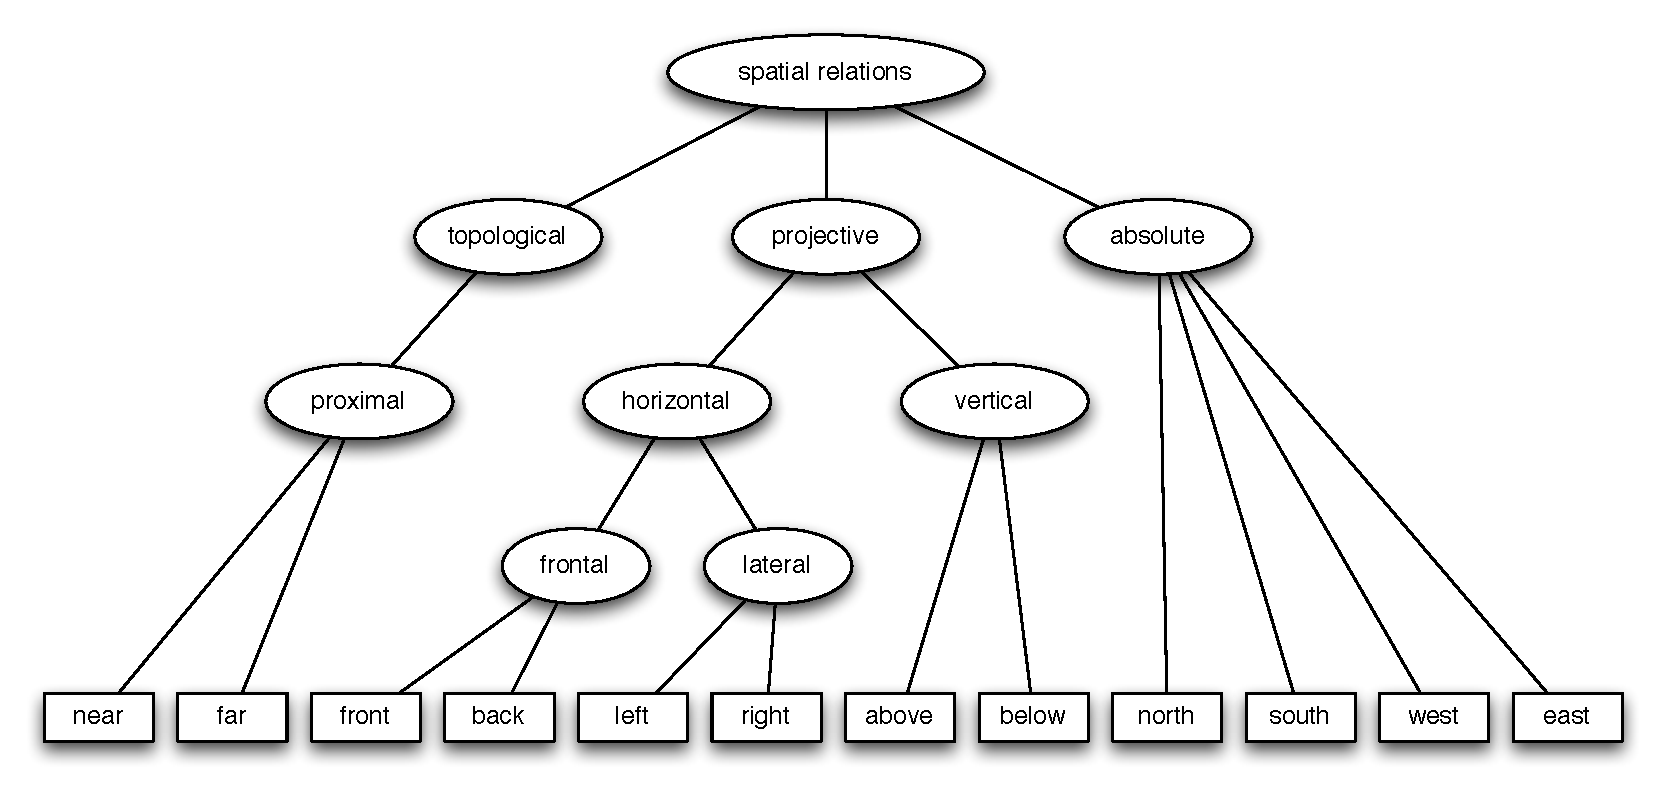
\includegraphics[width=\columnwidth]{figs/spatial-relations-taxonomy}
\label{f:spatial-relations-taxonomy}
\caption[Taxonomy of spatial relations in German.]{%
Taxonomy of spatial relations discussed in this book.
The rectangular items refer to the spatial terms used for denoting
the relations. Since in German spatial relations can be expressed in
different lexical classes and word forms, English
equivalents are used as placeholder.}
%\end{figure}
\end{sidewaysfigure}

Spatial relations take different syntactic forms in German. 
All of the projective terms, for instance, can be expressed in different 
lexical classes, most prominently as adjectives, adverbs and prepositions. 
For example, the projective term \textit{vor} can appear as adjective as in 
\REF{e:5:der-vordere-block}, as adverb as in \REF{e:5:der-block-vorne} 
and as preposition as in \REF{e:5:der-block-vor-der-kiste}. 
\is{adjectives}
\ea
\label{e:5:der-vordere-block}
\gll der vordere Block\\
the.{\NOM} front.{\ADJ}.{\NOM} block.{\NOM} \\
\glt `The front block'\\
%\glend
\z
\ea
\label{e:5:der-block-vorne}
\gll der Block vorne\\
the block.{\NOM} {in the front.{\ADV}} \\
\glt `The front block'\\
%\glend
\z
\ea
\label{e:5:der-block-vor-der-kiste}
\gll der Block vor der Kiste\\
the.{\NOM} block.{\NOM} front.{\PREP} the.{\DAT} box.{\DAT} \\
\glt `The block in front of the box.'\\
%\glend
\z

The different lexical classes carry with them different 
syntactic functions, e.g. adjectives can function as modifiers
in determined adjective noun phrases, prepositions are followed
by noun phrases and in German govern case.  
But each lexical class is also connected 
to a different semantic interpretation. In particular, there is 
a tight connection between the lexical class and specific spatial 
construal operations that govern how precisely the spatial relation is
to be applied. The meaning
of a projective category when used as an adjective is to filter objects 
\citep{tenbrink2007space}\index{Tenbrink, T.}, whereas when used as preposition the 
meaning is to construct a region \citep{klabunde1999logic}\index{Klabunde, R.}. 
For instance, the following phrase \REF{e:5:stelle-den-stuhl-vor-den-schrank} uses the projective category
front to construct a region to which one is asked to put a chair. 
Unlike in the adjective case, the region is not used to modify
or filter, rather the region is necessarily empty in order for the chair to be put there. 

\ea
\label{e:5:stelle-den-stuhl-vor-den-schrank}
\gll Stelle den Stuhl vor den Schrank!\\
Put the chair front.{\PREP} the cupboard\\
\glt `Put the chair in front of the cupboard!'\\
%\glend
\z

%%%%%%%%%%%%%%%%%%%%%%%%%%%%%%%%%%%%
%\paragraph*{Prepositions}
Another important difference between spatial adjectives and spatial adverbs and prepositions is the potential
for \textsc{reference objects} or \textsc{landmarks}. Example 
\REF{e:5:der-block-vor-der-kiste} relates a \textsc{located object}, also called
``figure'' \citep{talmy2000toward2}\index{Talmy, L.} and ``trajector'' \citep{vandeloise1991spatial}\index{Vandeloise, C.}
to a reference object, also called ``landmark'' \citep{vandeloise1991spatial}\index{Vandeloise, C.}, 
``relatum'' \citep{tenbrink2007space}\index{Tenbrink, T.} or ``ground'' \citep{talmy2000toward2}\index{Talmy, L.}.
If a spatial term is used prepositionally as in 
\REF{e:5:der-block-vor-der-kiste}, both the spatial relation, in this case 
\textit{vor}, and the landmark \textit{Kiste} (`box'), are expressed in the 
prepositional phrase itself. \is{prepositions}

%%%%%%%%%%%%%%%%%%%%%%%%%%%%%%%%%%%%
%\paragraph*{Adverbs}
A third possible lexical class, in which spatial relations partake, are adverbs. \is{adverbs}
Spatial adverbs can be accompanied
by a prepositional phrase, as in \REF{e:5:der-block-vorne-in-der-kiste}--\REF{e:5:der-block-links-von-der-kiste}:
\ea
\label{e:5:der-block-vorne-in-der-kiste}
\gll der Block vorne in der Kiste\\
the.{\NOM} block.{\NOM} front.{\ADV} of.{\PREP} the.{\DAT} box.{\DAT}\\
\glt `The block in the front of the box'\\
%\glend
\z
\ea
\label{e:5:der-block-links-von-der-kiste}
\gll der Block links von der Kiste\\
the.{\NOM} block.{\NOM} left.{\ADV} of.{\PREP} the.{\DAT} box.{\DAT}\\
\glt `The block to the left of the box'\\
%\glend
\z
The prepositional phrases \textit{in der Kiste} and \textit{von der Kiste}  both introduce
a landmark which, via
the spatial term, relates to the figure, in this case \textit{der Block}. The two different prepositions \textit{in} and \textit{von}
denote whether the relation referred to by the spatial term is \textsc{internal} 
to the landmark or \textsc{external}. In the case of \textit{von}, the spatial
region denoted by the projective adverb, e.g. \textit{links} (`left'), is external to the 
landmark, whereas in the case of \textit{in} the region lies within the landmark. 
The projective 
adverbs \textit{links} (`left') and \textit{rechts} (`right') can be followed both by 
\textit{von} and \textit{in} prepositional phrases, hence they can have an internal
and external reading. The projective adverbs \textit{vorne} (`front') 
and \textit{hinten} (`back') can only be extended by \textit{in} prepositional phrases. 
The vertical projective adverbs \textit{oben} (`above') and \textit{unten} (`below')
elicit internal readings. Again differences in semantic processing are 
syntactically marked, in the case of adverbs by prepositional phrases
that complement the adverb.

%\begin{figure}
%\label{f:region-external-vs-internal}
%\caption[Internal vs external regions.]{TODO: figure}
%\end{figure}

%%%%%%%%%%%%%%%%%%%%%%%%%%%%%%%%%%%%
%\paragraph*{Perspective Marking}
The last important component of spatial language considered in this book
is perspective marking. The following two example feature perspective markers. In \REF{e:5:der-block-vorne-von-dir-aus} an adverb is perspective marked, in \REF{e:5:der-block-links-der-kiste-von-dir-aus} a prepositional
phrase is perspective marked.
\ea
\label{e:5:der-block-vorne-von-dir-aus}
\gll der Block vorne von dir aus\\
the.{\NOM} block.{\NOM} front.{\ADV} from.{\PREP} the.{\DAT} box.{\DAT} \\
\glt `The block in front from your perspective'\\
%\glend
\z
\ea
\label{e:5:der-block-links-der-kiste-von-dir-aus}
\gll der Block links der Kiste von dir aus\\
the.{\NOM} block.{\NOM} left.{\PREP} the.{\GEN} box.{\GEN} from.{\PREP} your.{\DAT} perspective\\
\glt `The block to the left of the box from your perspective'\\
%\glend
\z
Perspective on a scene is important for particular interpretations
of spatial phrases, because it influences how the spatial scene and in 
particular the landmark is conceptualized. 


%\paragraph*{}

%\section{A Whole Systems Approach to German Spatial Language}
These few examples from German locative phrases show that 
we can analyze the syntax of spatial language 
fruitfully in terms of its spatial semantics. This resonates with 
theories of syntax which put the direct
mapping of syntax to semantics at the core of language processing, such as Construction Grammar.
The tight relationship between syntax and semantics is an important 
claim in this book which underlies the reconstruction efforts, and also
the evolution experiments. 

The first question I am focusing on is how to organize language processing.
That is, how semantics is encoded in words and grammar -- and vice versa.
However, this is not the full story. One needs to ground language in 
perception. Speakers need to be able to plan what they are going 
to say based on their communicative intention. Hearers must have machinery for
interpreting the utterance based on the spatial context. This widens the question
from how to organize the syntax and semantics interface to how to organize 
processing in a large array of systems comprising perception, conceptualization,
interpretation and also processing of syntax. In particular,
one has to identify the cognitive operations underlying the semantics of
German locative phrases and how these operations are used in conceptualization
of spatial scenes, as well as how conceptualization interacts with the
perception of spatial scenes.  The following section examine three main questions. 
First, what is the meaning of phrases such as
\textit{der Block links von der Box von dir aus} (`the block left of the box from your 
perspective', see \REF{e:5:der-block-links-der-kiste-von-dir-aus}) and
how can we formalize the semantic structure of these utterances?
What are the cognitive primitives that are necessary for modeling the 
semantics of spatial phrases in particular? Second, how does semantic structure get translated into 
words and grammatical relations and back? And thirdly how can agents 
autonomously conceptualize spatial scenes given
communicative goals and how can agents interpret semantic structure recovered in parsing
so that success in communication can be achieved?

%\bibliographystyle{diss}
%\bibliography{papers,space} 
%\end{document}

 \chapter{Spatial semantics}
\label{s:german-space-semantics}
So what is then the meaning of a phrase such as 
\textit{der Block links von der Kiste von dir aus} 
(`the block left of the box from your perspective')?
\figref{f:semantic-structure-der-block-links-der-kiste-von-dir-aus}
shows an IRL-network that agents autonomously construct to conceptualize
a particular spatial scene. The structure consists
of a set of cognitive operations that involve, for example, the construction of regions, 
the identification of landmarks, the application of perspective transformations and so on. But of course the network also contains references to spatial
categories, selectors, and other semantic entities that are processed by cognitive
operations. The following sections identify and describe the cognitive operations
and the semantic entities underlying locative utterances.

\begin{figure}
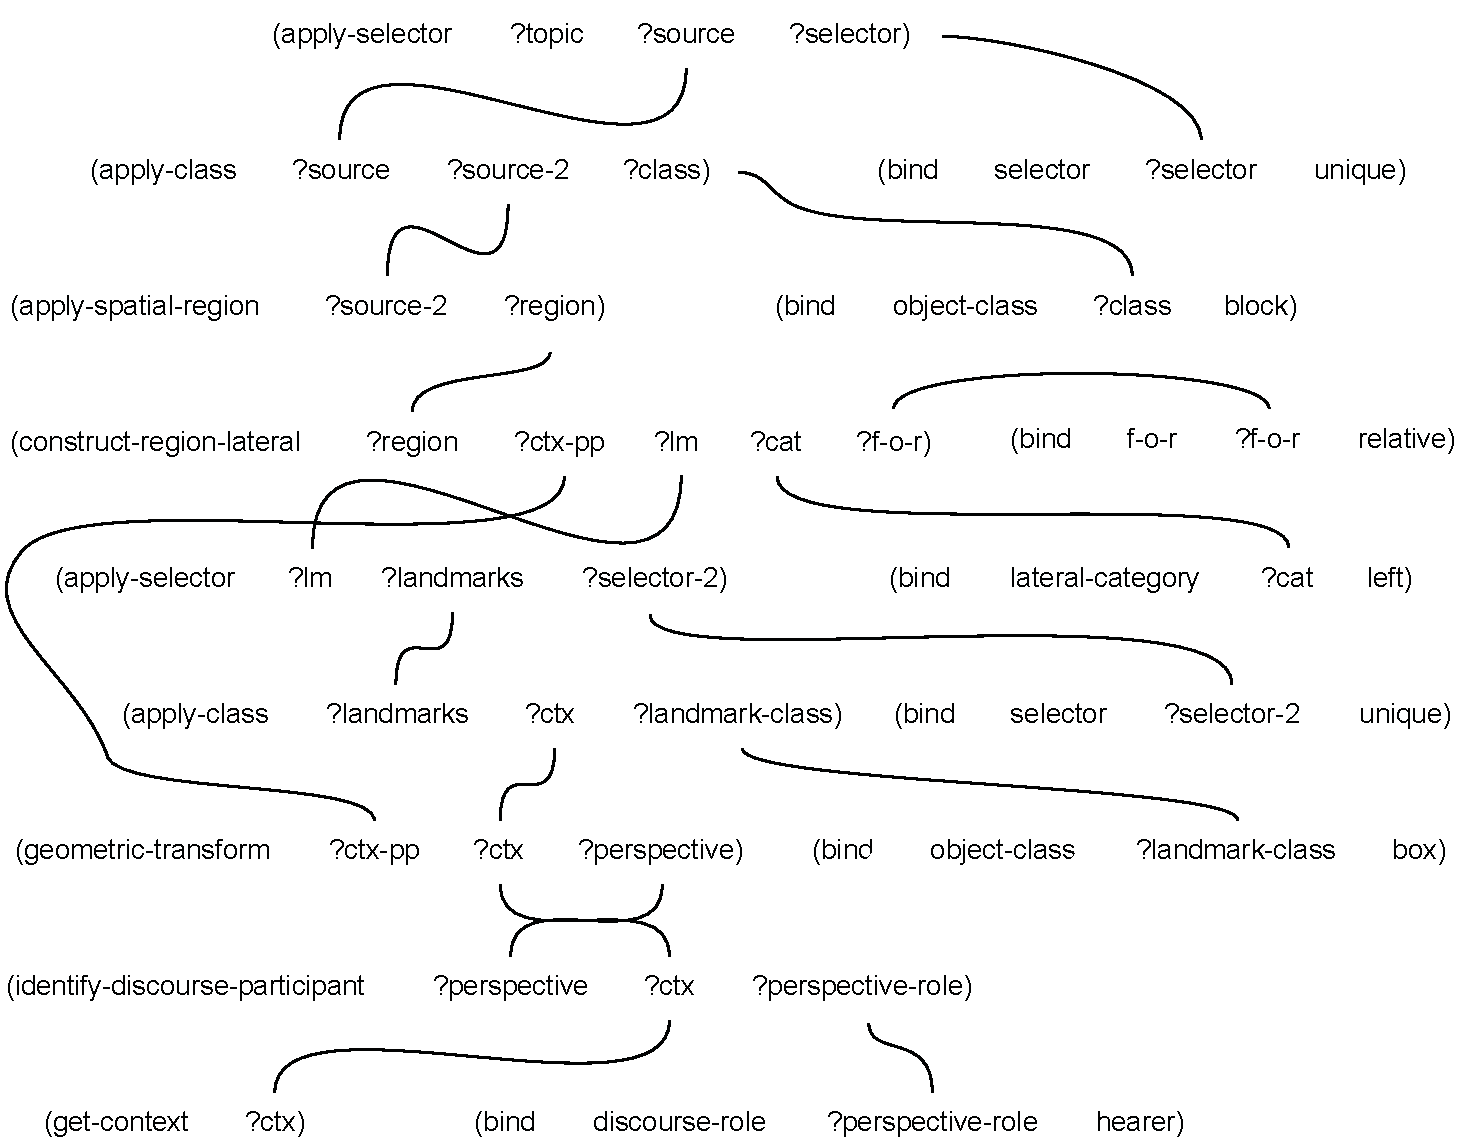
\includegraphics[width=\textwidth]{figs/semantic-structure-der-block-links-der-kiste-von-dir-aus}
\caption[Semantic structure of the phrase
\textit{der Block links von der Kiste von dir aus} 
(`the block left of the box from your perspective')]{%
An IRL-network representing the meaning of the phrase 
\textit{der Block links von der Kiste von dir aus} 
(`the block left of the box from your perspective')}
\label{f:semantic-structure-der-block-links-der-kiste-von-dir-aus}
\end{figure}

%%%%%%%%%%%%%%%%%%%%%%%%%%%%%%%%%%%%%
\section{Representing spatial relations}\is{spatial relation}
The semantics of spatial relations is the subject of ongoing debate. The 
key question is whether there is something like a 
\textsc{semantic core}\is{spatial relation!semantic core}  of 
spatial relations, i.e. a core meaning that 
abstracts from discourse situations as far as possible 
\citep{tenbrink2007space}\oldindex{Tenbrink, T.}, and what that 
semantic core should be. For many scholars, the semantic core of spatial 
relations is related to geometric 
properties \citep{herskovits1986language,eschenbach1999geometric,tenbrink2007space}\oldindex{Eschenbach, C.}\oldindex{Herskovits, A.}\oldindex{Tenbrink, T.}
in particular prototypical axis (directions) and distances defined using tools 
like lines, points, vectors, half-planes, etc. \citep{levinson1996language}\oldindex{Levinson, S. C.}. 
Particularly, projective relations, e.g. \textit{vor} (`front') have been studied 
in this respect and certainly the class of absolute relations, e.g. \textit{n\"ordlich} 
(`north'), can be conceived in these terms. For instance, 
\cite{herskovits1986language}\oldindex{Herskovits, A.}  describes the meaning 
of the spatial relation \textit{in front of} as graded concept with the frontal 
axis as the focal region. This conception links to another important property
of spatial language namely its inherent vagueness 
\citep{hall2008quantifying}\oldindex{Hall, M. M.}\oldindex{Jones, C. B.}.
Many of these proposals are rooted in a strand of psycholinguistic research that is concerned with
prototypes and prototypicality effects \citep{rosch1978principle}\oldindex{Rosch, E.}. 
Here, prototypes or prototypical points in the sensorimotor
space are used as representations for spatial categories
(for a similar approach to color, see \citealt{bleys2010phd}\oldindex{Bleys, J.}). 
For instance, the projective term \textit{links} (`left') can 
be interpreted for objects which relate to the reference object
by an angle of $90^\circ$ (prototypical left angle). The more the angle 
between the target object and the reference system deviates,
the less acceptable the spatial relation becomes \citep{tenbrink2005identifying,herskovits1986language,gapp1995angle}\oldindex{Gapp, K.}\oldindex{Tenbrink, T.}\oldindex{Herskovits, A.}. 

In this section I focus on the geometric properties of spatial relations 
and combine them with the prototype approach to spatial categorization. 
There are two features of the sensorimotor space which are of particular
importance for spatial categorization: distance and angle. Two objects 
always have a certain distance from each other, and if there is a
coordinate system available which supports rotation also angles 
between objects can be measured. 
Consequently, from a computational point of view, there are two 
important category types for representing the geometric properties 
of the German spatial relations discussed in this book {\footnotesize\tt angular-category},\enlargethispage{1\baselineskip}
which represent prototypical angles and {\footnotesize\tt proximal-category},
which represent prototypical distances (see Figure \ref{f:category-hierarchy} for an overview).\is{spatial relation!proximal}

\begin{figure}
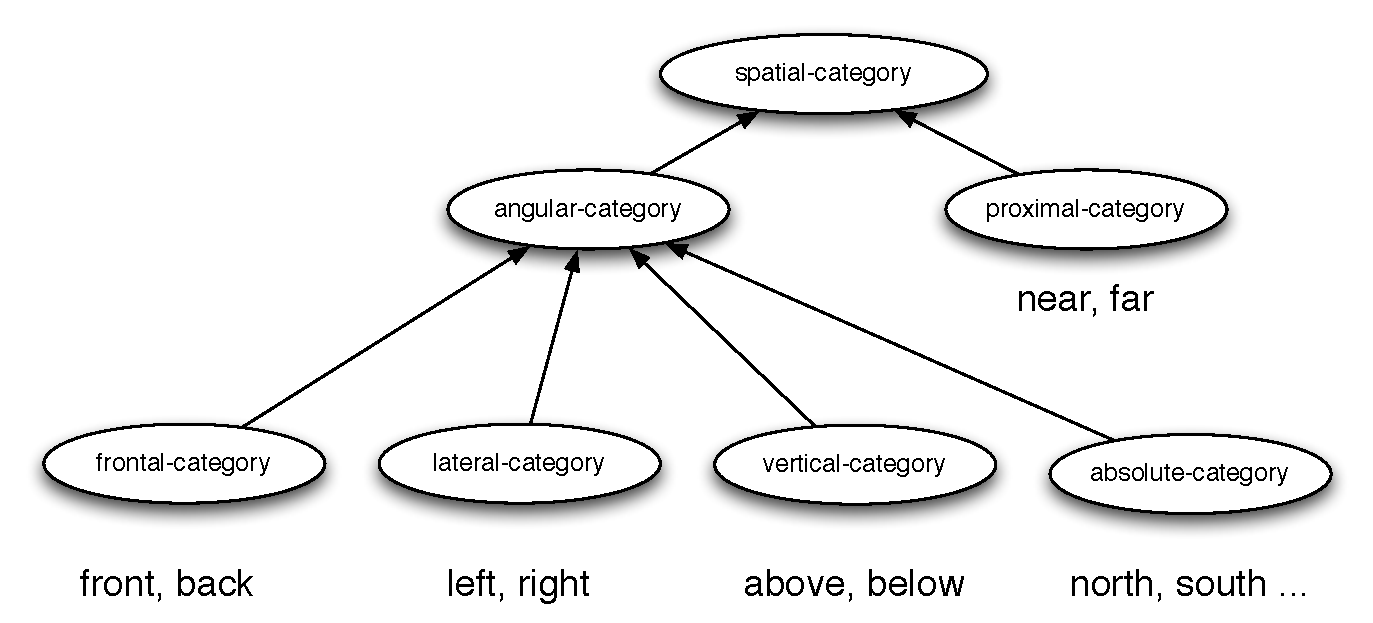
\includegraphics[width=1\columnwidth]{figs/category-hierarchy.pdf}
\caption[Category type hierarchy]{Category type hierarchy 
used in semantic processing}
\label{f:category-hierarchy}
\end{figure}

\subsection{Angular relations} 
The core semantics of spatial relations is represented
using functions that map a particular input location to the applicability degree 
of a particular category. For prototype based spatial categories 
degree of applicability amounts to similarity in some spatial dimension, 
e.g. in the angular dimension for angular relations. 
Projective and absolute relations are\is{spatial relation!projective}\is{spatial relation!absolute}\is{spatial relation!angular}
examples of angular categories, with a focal region around the 
denoted axis. For instance, frontal categories have a high degree of applicability
along the frontal axis. Whereas lateral categories have a high 
degree of applicability along the left and right axis. Similarly, 
absolute categories have high values of applicability
in their respective direction (see \figref{f:prototypical-spatial-relations} 
for an overview). In other words, for angular categories, 
similarity of some location to the category depends on the distance
of angles. In order to get a similarity function $\operatorname{sim}_{a} \in [0,1]$
the angle distance is wrapped in an exponential decay envelope 
and weighted by a $\sigma$ which steers the steepness of the 
exponential decay. High values for $\sigma$ correspond to a slow decay 
in similarity the bigger the angular distance, whereas low values for $\sigma$ 
correspond to a sharper decline in similarity.
Consequently, the following equations defines the degree of applicability given a
location $l$ and an angular category $c$, as the angular distance 
between $c$ and $l$, weighted by $\sigma$ and run through an exponential
decay.
\begin{eqnarray}
\label{e:angular-category-similarity}
\operatorname{sim}_{a}(l,c)&:=&e^{-\frac{1}{2 \sigma_c} d_a(l,c)}\\
\label{e:angular-distance}
d_a(l,c)&:=&|a_l - a_c|
\end{eqnarray}
In this definition $a_l$ denotes the angle of the position of location $l$ 
to the coordinate center and $a_c$ denotes the prototypical angle of the 
category $c$. Given this definition, one can go ahead and define 
angular categories, in particular I need to define the prototypical
angle for each angular category and the $\sigma$. 
Examples of definitions of angular spatial relations are 
depicted in \figref{f:prototypical-spatial-relations}. 


\subsection{Proximal relations} 
Proximal relations relate to some prototypical
distance. Two relations are modeled: {\footnotesize\tt near} and 
{\footnotesize\tt far}. The only difference to the definition of angular
categories is that proximal relations rely on the distance channel.
\begin{eqnarray}
\label{e:proximal-category-similarity}
\operatorname{sim}_{d}(l,c)&:=&e^{-\frac{1}{2 \sigma_c} d_d(l,c)}\\
\label{e:proximal-distance}
d_d(l,c)&:=&|d_l-d_c|
\end{eqnarray}
In this definition $d_l$ denotes the distance of the location $l$ 
to the coordinate center and $d_c$ denotes the prototypical 
distance of the category $c$.

\begin{figure}
\label{f:prototypical-spatial-relations}
\begin{center}
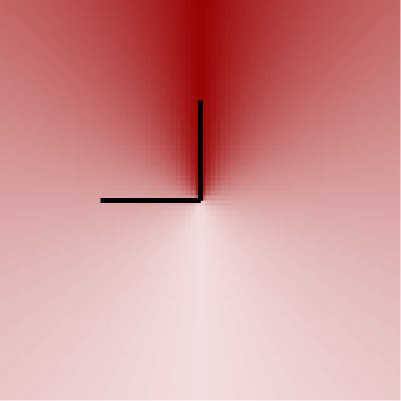
\includegraphics[width=0.15\columnwidth]{figs/categorization-front.jpg}

\includegraphics[width=0.15\columnwidth]{figs/categorization-back.jpg}
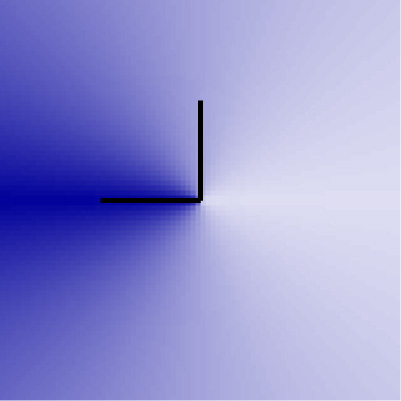
\includegraphics[width=0.15\columnwidth]{figs/categorization-left.jpg}

\includegraphics[width=0.15\columnwidth]{figs/categorization-right.jpg}
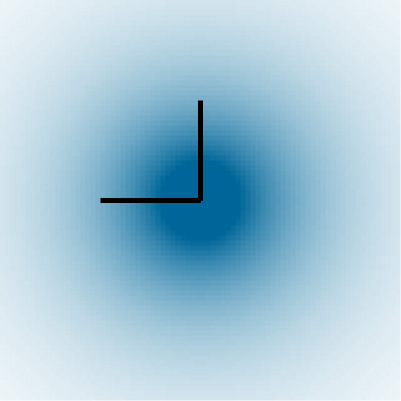
\includegraphics[width=0.15\columnwidth]{figs/categorization-near.jpg}

\includegraphics[width=0.15\columnwidth]{figs/categorization-far.jpg}
\end{center}
\caption[Degree of acceptability for projective and proximal categories.]{%
Degrees of acceptability shown for prototypical representation of frontal 
and lateral projective categories. From left to right {\footnotesize\tt front}, {\footnotesize\tt back},
 {\footnotesize\tt left}, {\footnotesize\tt right}, {\footnotesize\tt near} and {\footnotesize\tt far} are shown. 
 The opacity of each color denotes acceptability for a particular location in space ($x$-axes and $y$-axes 
 each run from $-2000.0$ to $2000.0$). 
 {\footnotesize\tt Front}, for instance, shows a strong acceptability along the $x$-axes. Definitions of 
categories are $a_{\mathtt{\footnotesize front}}=0.0$, $a_{\mathtt{\footnotesize back}}=\pi$, 
$a_{\mathtt{\footnotesize left}}=\frac{\pi}{2}$ and $a_\mathtt{{\footnotesize left}}=-\frac{\pi}{2}$ and
$\sigma_{\mathtt{\footnotesize front}}=\sigma_{\mathtt{\footnotesize\ back}}=\sigma_\mathtt{{\footnotesize left}}=\sigma_{\mathtt{\footnotesize right}} = 1.0$.
For absolute categories the same definitions exist with {\footnotesize\tt north} being defined like {\footnotesize\tt front}
and so forth.
The two proximal categories {\footnotesize\tt near} and {\footnotesize\tt far} are defined 
with $d_{\mathtt{\footnotesize near}}=0.0$, $a_{\mathtt{\footnotesize far}}=2000.0$ and 
$\sigma_{\mathtt{\footnotesize near}=700.0}$ and $\sigma_{\mathtt{\footnotesize far}}=1200.0$.}
\end{figure}


%%%%%%%%%%%%%%%%%%%%%%%%%%%%%%%%%%%%%
\section{Applying spatial relations}\is{spatial relation!regions}
Prepositionally and adverbially expressed spatial relations denote 
\textsc{spatial regions} which are always related to some reference object.
For instance, in the phrase \textit{der block links der Kiste} (`the block to the left
of the box') an object \textit{der Block} (`the block') is related to the landmark 
\textit{die Kiste} (`the box') via the spatial category \textit{links} (`left'). 
The information about which category is used and which landmark
is referred to is packaged in a spatial region.
In order to represent the difference between the construction of a region
as for instance denoted by the prepositional phrase \textit{vor der Kiste}
(`in front of the box') and the application of that region to filter objects,
as in the phrase \textit{der Block vor der Kiste} (`the block in front of the region'),
in other words in order to represent spatial relations, spatial 
processing is split into two distinct semantic operations. One operation
constructs the region and packages the particular landmark and the particular
spatial category, the other applies the region as a spatial relation 
to the objects available in the context.

\subsection{Spatial regions and spatial relations}
Proximal regions are computed based on the distance prototype of the 
corresponding category and the landmark. The semantic operation
{\footnotesize\tt construct-region-proximal} therefore constructs a specific 
region based on a spatial category and a landmark. 
The right image in \figref{f:apply-proximal-region} 
shows an example of a proximal region. 

\definition{Semantic operation}{construct-region-proximal}
\begin{explanation}{description}
Computes a proximal region based on the landmark.
\end{explanation}
\begin{explanation}{arguments}
{\footnotesize\verb+?spatial-region+} (of type spatial-region) \\
{\footnotesize\verb+?source-set+} (of type entity-set) \\
{\footnotesize\verb+?landmark+} (of type point)\\
{\footnotesize\verb+?category+} (of type proximal-category)
\vspace{0.3cm}
\end{explanation}

The other operation needed for applying a region is called 
{\footnotesize\tt apply-spatial-region}. This operation computes the similarity of 
every object in the context, given a region constructed, for instance by the 
operation {\footnotesize\tt construct-proximal-region}. For the case of 
a proximal region, this involves (1) transforming the context so
that the landmark is at the center of origin of the coordinate system
and (2) applying the similarity function defined in Equation 
\ref{e:proximal-category-similarity}. This operation in many ways
acts as a classifier such as the semantic operations for {\footnotesize\tt color}
and {\footnotesize\tt object-class} described in \chapref{s:irl}.\enlargethispage{1\baselineskip}
For each object in the source set the similarity of this object to the 
spatial region is computed, based on the constituents of the region,
e.g. which category and which landmark was used to define the region.
This similarity is combined with the other computed similarities for
the object (see \chapref{s:irl} for description). 
The operation {\footnotesize\tt apply-region-filter} 
is general enough to be applicable to all regions, including projective and absolute 
regions whose description is to follow.\footnote{This operation can
be very general because its implementation defers different
methods of computing similarity for different category types
using the method dispatching facility of lisp.}

\definition{Semantic operation}{apply-spatial-region}
\begin{explanation}{description}
Applies a spatial region, by computing the similarity of the region
with every entity in {\footnotesize\verb+?source-set+}.
\end{explanation}
\begin{explanation}{arguments}
{\footnotesize\verb+?target-set+} (of type entity-set) \\
{\footnotesize\verb+?source-set+} (of type entity-set) \\
{\footnotesize\verb+?region+} (of type spatial-region)
\vspace{0.3cm}
\end{explanation}

An example of the interplay of the operations 
{\footnotesize\tt construct-region-proximal} 
and {\footnotesize\tt apply-region-filter} for
a spatial scene can be seen in
\figref{f:apply-proximal-region}. The following table 
summarizes the similarities computed when applying 
the region to the context (\figref{f:apply-proximal-region}
left).

\begin{center}
\begin{tabular}{lSS}
\lsptoprule
object & \multicolumn{1}{l}{distance (mm)} & \multicolumn{1}{l}{similarity} \\
\midrule
robot-1 & 1041.02 & 0.48 \\
robot-2 & 1224.53 & 0.42 \\
box-1 & 0.00 & 0.00\\
obj-266 & 419.97 & 0.74\\
obj-265 & 938.99 & 0.51 \\
\lspbottomrule
\end{tabular}
\end{center}


\begin{figure}
\begin{centering}
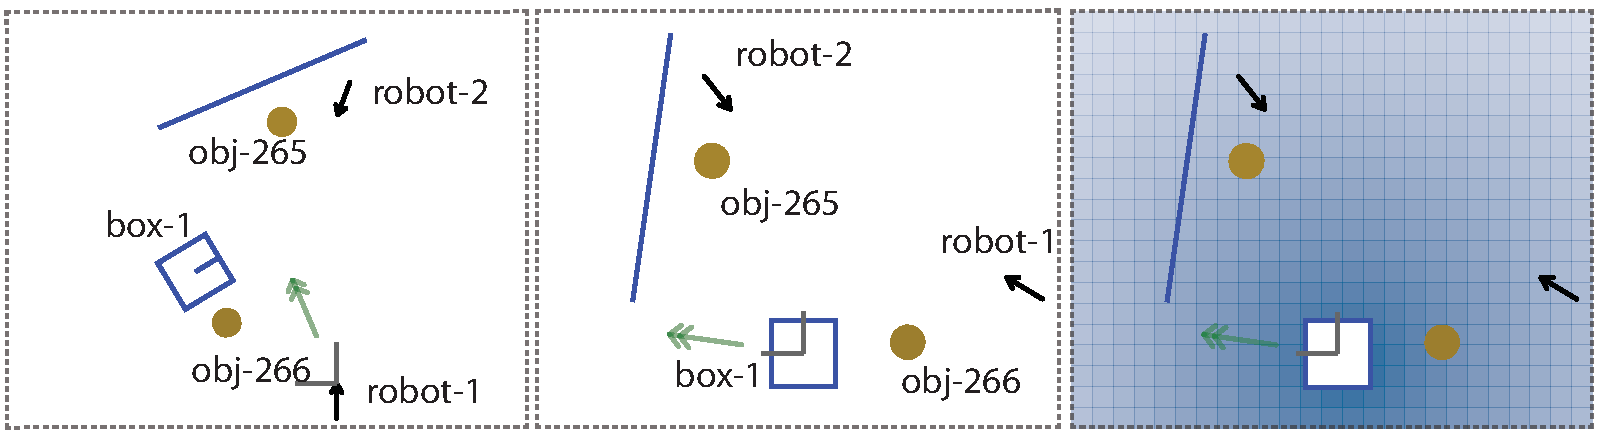
\includegraphics[width=\textwidth]{figs/space-scene-3-speaker-apply-proximal-region.pdf}
\end{centering}
\caption[Steps involved in applying a spatial relations.]
{When a region is applied, first, the context (left figure) is transformed so that
the landmark is at the origin of the coordinate system (middle figure) which is followed by the 
application of the spatial relation (right figure). Here, these steps are 
depicted for the category {\footnotesize\tt near} and the landmark {\footnotesize\tt box-1}.}
\label{f:apply-proximal-region}
\end{figure}

\section{Frames of reference}\is{frames of reference}
Projective and absolute relations are defined in terms of focal directions.
Consequently, for these kinds of relations the rotation of the landmark 
is an important issue determining the precise applicability of 
these relationships. For example, what is considered the front direction 
of a landmark has a direct effect on what is considered a frontal region. It turns out
that there is considerable amount of choice when it comes to how to\enlargethispage{1\baselineskip}
define the rotation of the landmark. The combination 
of a coordinate system, in particular its rotation, with a landmark is 
called \textsc{reference system}. Reference systems 
have been dealt with in great detail in cognitive semantics and 
psycholinguistics under the term \textsc{frame of reference}. 
\cite{levinson1996language,levinson2003space}\oldindex{Levinson, S. C.} identifies 
three possible frames of reference: \textsc{intrinsic}, \textsc{relative} 
and \textsc{absolute}, all of which denote a particular way of construing 
a landmark for spatial relationships involving direction. 
In German all three frames of reference are possible.


\begin{description}
\item[Intrinsic frame of reference]\is{frames of reference!intrinsic}
The intrinsic frame of reference is an object centered coordinate 
system, meaning that projective categories are applied to the 
reference object based on particular sides of the object, which 
are construed as front, back, left and right. Hence, those objects 
that have something that can be considered as their front 
(with other sides, identifiable as well, e.g., left, right and back) 
are eligible to be used as landmarks with an intrinsic frame of 
reference. Examples of such objects are television sets, where 
the front is the screen, or houses, where the front is the main 
entrance or street access, and so forth.
\item[Relative frame of reference]
The relative frame of reference is a perspective based coordinate 
system. (See \figref{f:frames-of-reference} for a graphical 
explanation.) Instead of relying on intrinsic features of the 
reference object for determining the particular layout of the 
coordinate system, the rotation of the coordinate system is 
determined by its angle to an explicitly or implicitly given 
perspective. Hence, the front of an object is induced by the\enlargethispage{1\baselineskip} 
particular perspective on the scene. For example, \textit{vor dem 
Baum} (`in front of the tree') implicitly refers to a perspective, 
because trees do not have an intrinsically determined front, and 
it is the position of the observer together with the position of the 
tree that designates the precise region denoted as front.
\item[Absolute frame of reference] Absolute frames of reference construe 
the landmark using an external rotation. Neither intrinsic 
properties nor the perspective on the landmark determine the layout 
of the coordinate system, but rather geocentric features of the 
environment, for instance cardinal directions as in 
\textit{n\"ordlich} (`north') or the direction of gravity as in \textit{\"uber} (`above')
govern what the precise layout of the reference system is.
\end{description} 

\begin{figure}
\begin{center}
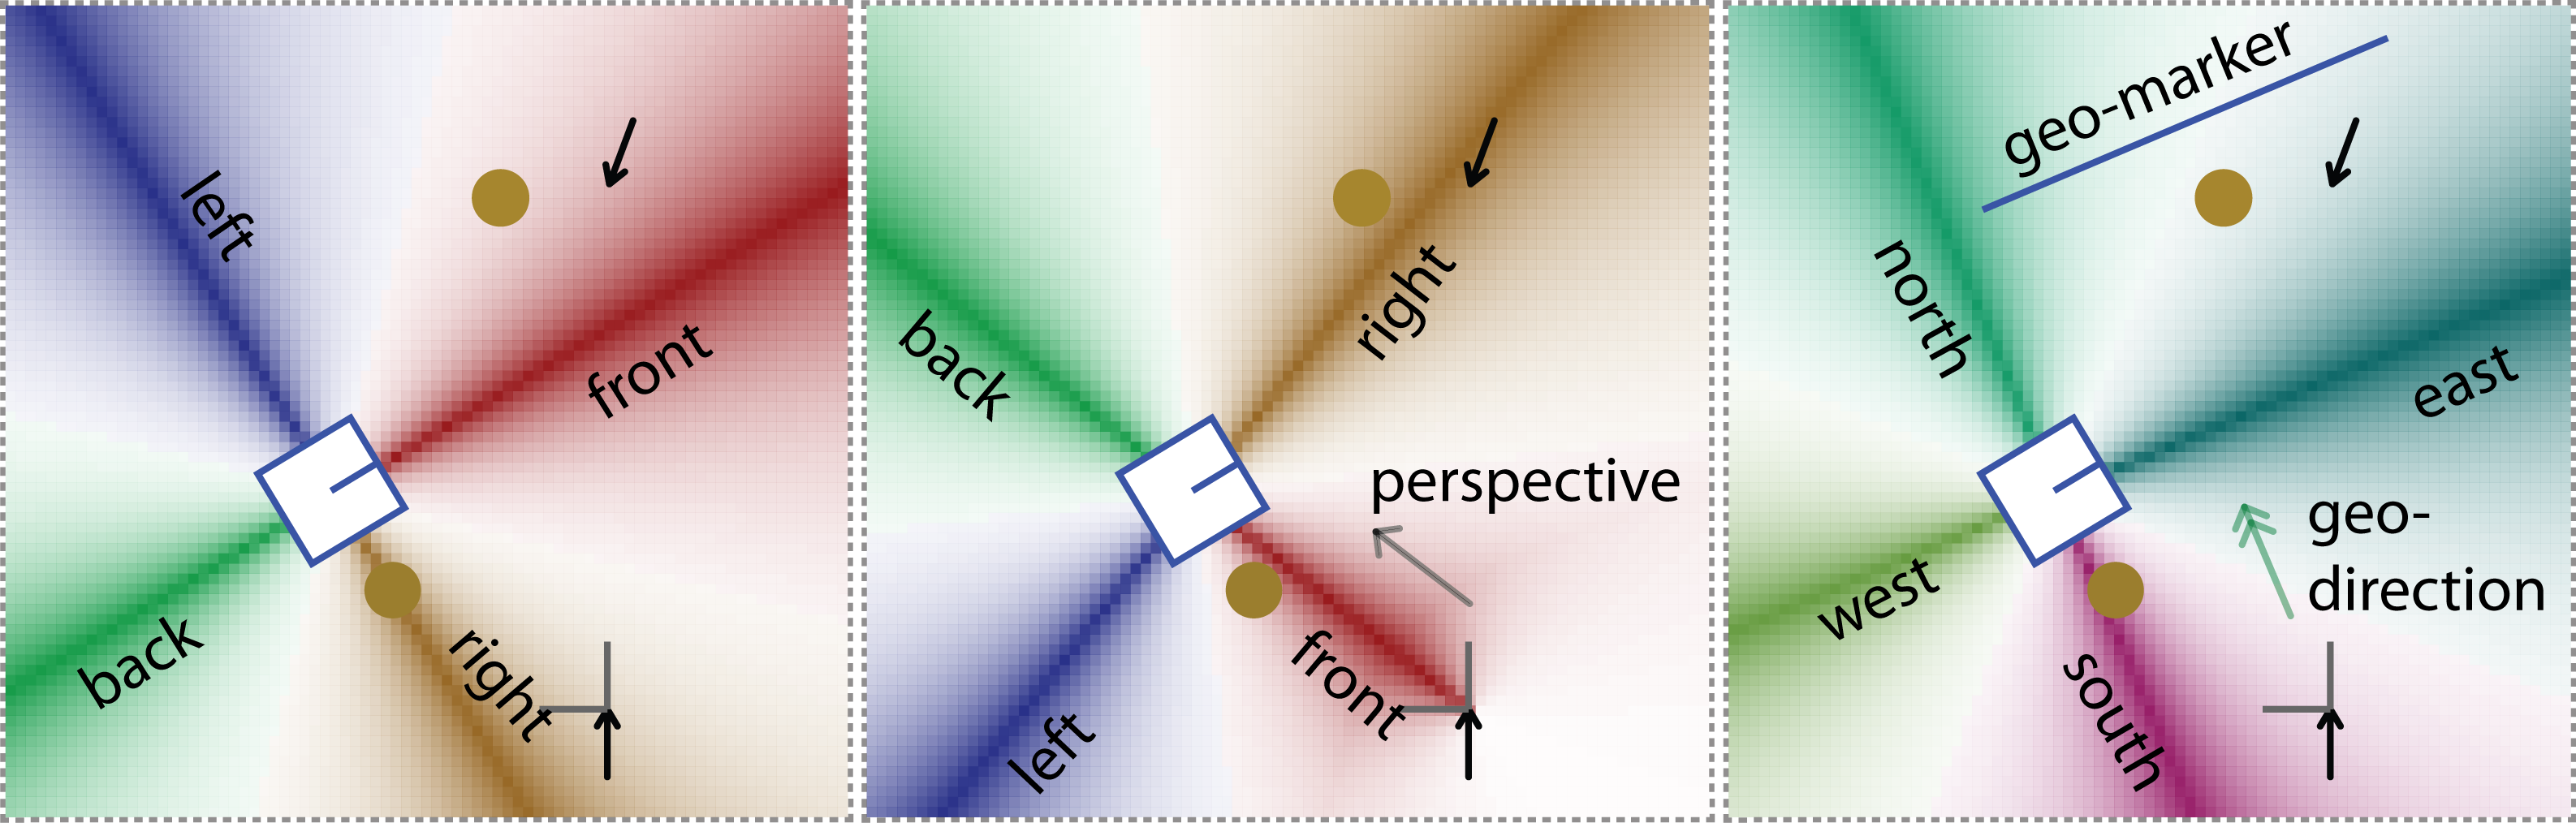
\includegraphics[width=1\columnwidth]{figs/space-scene-3-frames-of-reference.png}
\end{center}
\caption[Spatial relations and frames of reference.]
{Frames of reference have a profound effect on spatial relations. In all three
pictures spatial relations are shown with {\footnotesize\tt box-1} as reference object. The left
figure shows the landmark construed with an intrinsic frame of reference which
orients the coordinate system such that the front of the landmark 
(little blue line in the landmark) corresponds to the frontal spatial relation with
left, right and back projective relations aligned accordingly. The middle figure
shows the same landmark, but with a relative frame of reference constructed
from the perspective of robot {\footnotesize\tt robot-1} which entails that frontness 
corresponds to a region between the perspective and the landmark. 
Left and right in relative frames of reference are aligned not with respect to
front, but rather are parallel to the left and right side of the perspective 
{\footnotesize\tt robot-1}.
The right figure shows an absolute frame of reference applied to the landmark 
{\footnotesize\tt box-1}. Cardinal directions are aligned based on a geocentric direction
induced on the scene by a marker.\is{frames of reference!relative}}
\label{f:frames-of-reference}
\end{figure}


The differences in processing frames of reference are captured using 
distinct semantic operations. In other words, absolute relationships, 
such as \textit{n\"ordlich} (`north') or \textit{\"uber}  (`above') demand other semantic 
operations as relative and intrinsic ones. For instance, 
processing of phrases involving absolute regions, e.g. \textit{n\"ordlich}
(`north'), is represented using the {\footnotesize\tt construct-region-absolute} operation, 
which takes a landmark and transforms the context with respect to the 
landmark, subsequently applying a rotation that follows from a geocentric direction. 
Some of the spatial scenes recorded by the robots feature
a geocentric marker on the wall. The direction towards this marker
defines the direction to the north. Figure \ref{f:frames-of-reference} 
gives an example.

\is{frames of reference!absolute}
\definition{Semantic operation}{construct-region-absolute}
\begin{explanation}{description}
Computes an absolute region based on the landmark
and the absolute frame of reference which must be available
in source set.
\end{explanation}
\begin{explanation}{arguments}
{\footnotesize\verb+?spatial-region+} (of type spatial-region) \\
{\footnotesize\verb+?source-set+} (of type entity-set) \\
{\footnotesize\verb+?landmark+} (of type point)\\
{\footnotesize\verb+?category+} (of type absolute-category)
\vspace{0.3cm}
\end{explanation}

Frontal prepositions, e.g., \textit{vor} (`front') and \textit{hinter} (`back'), can have
both intrinsic and relative readings. Both readings are incorporated
into a single operation, which construes the landmark both
in relative and intrinsic way signified by an additional parameter
of type {\footnotesize\tt f-o-r} (frame of reference) to the operation.
For the relative reading the perspective on the scene additionally
influences the layout of the region. The viewpoint on
the scene constrains front regions in such a way that
only those locations which are between the perspective and
the landmark have a high degree of applicability.

\definition{Semantic operation}{construct-region-frontal}
\begin{explanation}{description}
Computes a frontal region based on the landmark
and the relative or intrinsic frame of reference.
\end{explanation}
\begin{explanation}{arguments}
{\footnotesize\verb+?spatial-region+} (of type spatial-region) \\
{\footnotesize\verb+?source-set+} (of type entity-set) \\
{\footnotesize\verb+?landmark+} (of type point)\\
{\footnotesize\verb+?f-o-r+} (of type f-o-r)\\
{\footnotesize\verb+?category+} (of type frontal-category)
\vspace{0.3cm}
\end{explanation}

Vertical relations can be construed with an absolute, relative\enlargethispage{1\baselineskip}
or intrinsic frame of reference. In the case of absolute frames
of reference the orientation is derived from gravity. For the purpose
of this book only absolute frames of reference readings are
implemented in the operation {\footnotesize\tt construct-region-vertical}.


%%%%%%%%%%%%%%%%%%%%%%%%%%%%%%%%%%%%%
\section{Internal and external regions}\is{spatial relation!internal}\is{spatial relation!external}
Another line of processing distinctions can be made between internal 
and external relations. \textit{North} and \textit{south}, but also prepositional use
of \textit{front}, e.g. \textit{vor}, are referring to external regions, that is the
region lies outside of the landmark. Internal regions on the other
hand lie inside the reference object. Adverbs such as \textit{vorne} (`front')
denote such regions inside the landmark. Consequently, they require
separate treatment and there is a specific operation
for handling the internal processing of frontal relations 
{\footnotesize\tt construct-region-frontal-internal}.

\definition{Semantic operation}{construct-region-frontal-internal}
\begin{explanation}{description}
Computes an internal frontal region based on the landmark
and the relative or intrinsic frame of reference.
\end{explanation}
\begin{explanation}{arguments}
{\footnotesize\verb+?spatial-region+} (of type spatial-region) \\
{\footnotesize\verb+?source-set+} (of type entity-set) \\
{\footnotesize\verb+?landmark+} (of type point)\\
{\footnotesize\verb+?f-o-r+} (of type f-o-r)\\
{\footnotesize\verb+?category+} (of type frontal-category)
\vspace{0.3cm}
\end{explanation}

Internal lateral regions are not clearly marked in syntax. 
While lateral prepositions clearly denote an external region, 
lateral adverbs can be used more varied which becomes apparent
since they can be complemented both by \textit{von} headed prepositonal
phrases, as well as \textit{in} headed prepositional phrases.
In other words, the interpretation of an adverb depends
on the complement. If there is no complement both readings
internal and external are possible. 

\definition{Semantic operation}{construct-region-lateral}
\begin{explanation}{description}
Computes an internal frontal region based on the landmark
and the relative or intrinsic frame of reference.
\end{explanation}
\begin{explanation}{arguments}
{\footnotesize\verb+?spatial-region+} (of type spatial-region) \\
{\footnotesize\verb+?source-set+} (of type entity-set) \\
{\footnotesize\verb+?landmark+} (of type point)\\
{\footnotesize\verb+?f-o-r+} (of type f-o-r)\\
{\footnotesize\verb+?category+} (of type frontal-category)\\
{\footnotesize\verb+?region-layout+} (of type region-layout)
\vspace{0.3cm}
\end{explanation}

%%%%%%%%%%%%%%%%%%%%%%%%%%%%%%%%%%%%
\begin{figure}
\begin{centering}
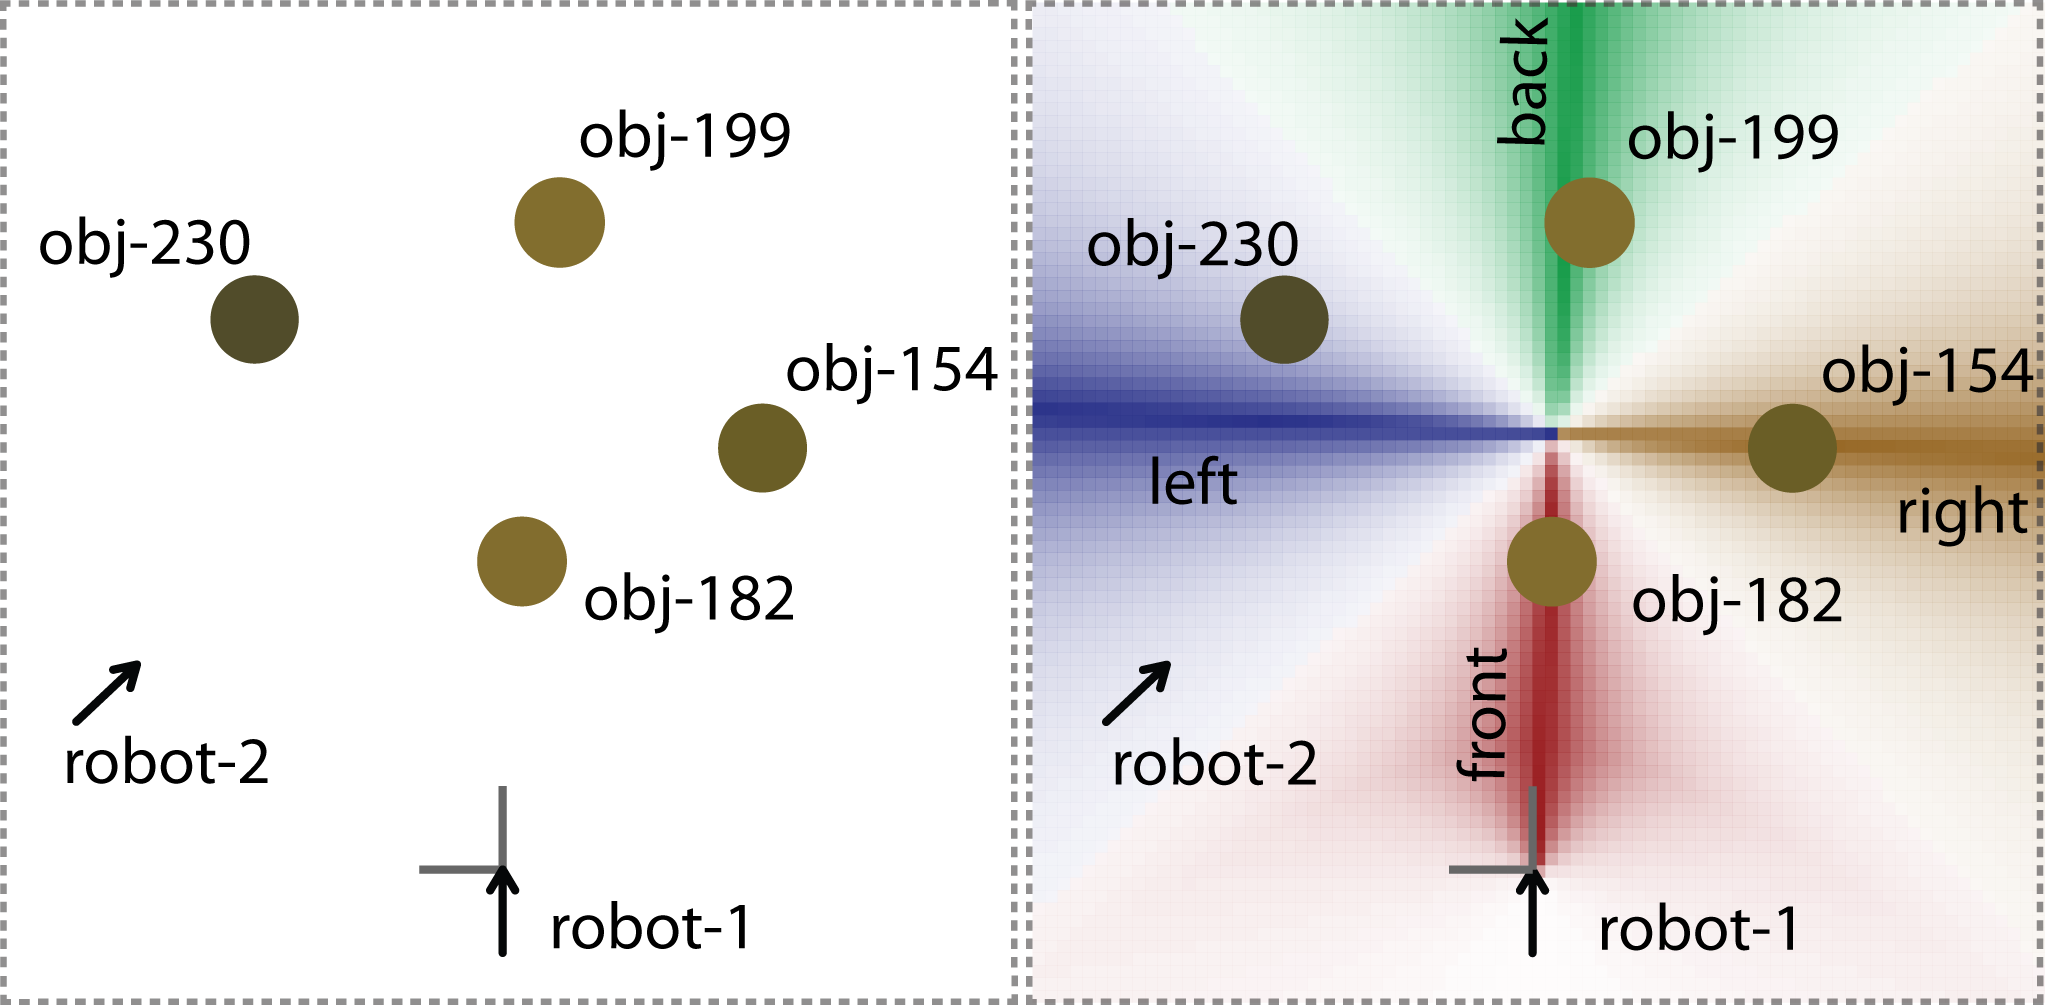
\includegraphics[width=0.7\columnwidth]{figs/space-scene-3483324847-group-based-reference.png}
\caption[Group-based reference explanation.]
{Group-based reference requires computing a landmark based on 
a group of objects. The centroid of the group of objects, in this case 
all blocks in the context, is construed using a relative frame of reference.
Consequently, object {\footnotesize\tt obj-182} could be described in German as 
\textit{der vordere Block} (`the front block').}
\label{f:6:space-scene-2}
\end{centering}
\end{figure}

\section{Group-based reference}\is{spatial relation!group-based reference}
The semantics of German spatial adjectives is best understood in terms of 
group-based reference.\footnote{Recent evidence \citep{moratz2006spatial}\oldindex{Moratz, R.}\oldindex{Tenbrink, T.} 
points to more variety in interpretation. For the purpose of this book, however,
I choose to model group-based semantics only.} In order for a group of objects 
to function as a reference object, the group needs to be construed as a landmark object, and in
particular its position needs to be established. One way of computing a position
for a group of objects, is to use the spatial centroid (center of mass) of the group 
as the position of the reference object. Additionally, a frame of reference, in other words
a rotation, needs to be chosen. This choice depends on the spatial relation. For
absolute relations the frame of reference is determined by an absolute 
frame of reference. In the absence of intrinsic features of the group of objects,
a relative frame of reference seems to be the natural choice, as a spatial group
of objects has no intrinsic front without including further constraints. 
Together, the centroid and the respective frame of reference sufficiently 
describe the reference system in order for spatial 
relations to be applied.

\definition{Semantic operation}{apply-spatial-category-group-based}
\begin{explanation}{description}
Applies the spatial category based on a group-based landmark. 
\end{explanation}
\begin{explanation}{arguments}
{\footnotesize\verb+?target-set+} (of type entity-set) \\
{\footnotesize\verb+?source-set+} (of type entity-set) \\
{\footnotesize\verb+?category+} (of type spatial-category)
\vspace{0.3cm}
\end{explanation}

Group-based reference offers a technical challenge of how to 
compute the group used for reference in the first place. Given that
all objects in the context are scored by successive operations, how can
a group of objects be established, in order to compute the
spatial centroid? For instance, in phrases like \textit{der linke block} (`the left block'),
the spatial adjective is part of a noun phrase, which primarily denotes the type of
objects that constitute a set, namely the set of all block which relates to 
the group that the reference should be based on.
The implementation of the semantic operation 
{\footnotesize\tt apply-spatial-category-group-based} relies on a well-known clustering algorithm
called $k$-means)\is{k-means@$k$-means} \citep{lloyd1982least}\oldindex{Lloyd, S.P.} in order to find the group 
of objects in the input set. The scores of all objects in the input set 
are used to divide the input set into two groups and all elements 
in the group with the higher score centroid are used to compute 
the spatial landmark. 

%%%%%%%%%%%%%%%%%%%%%%%%%%%%%%%%%%%%%
\section{Perspective marking}\is{perspective marking}

\begin{figure}
\begin{center}
% LARGE_PDF
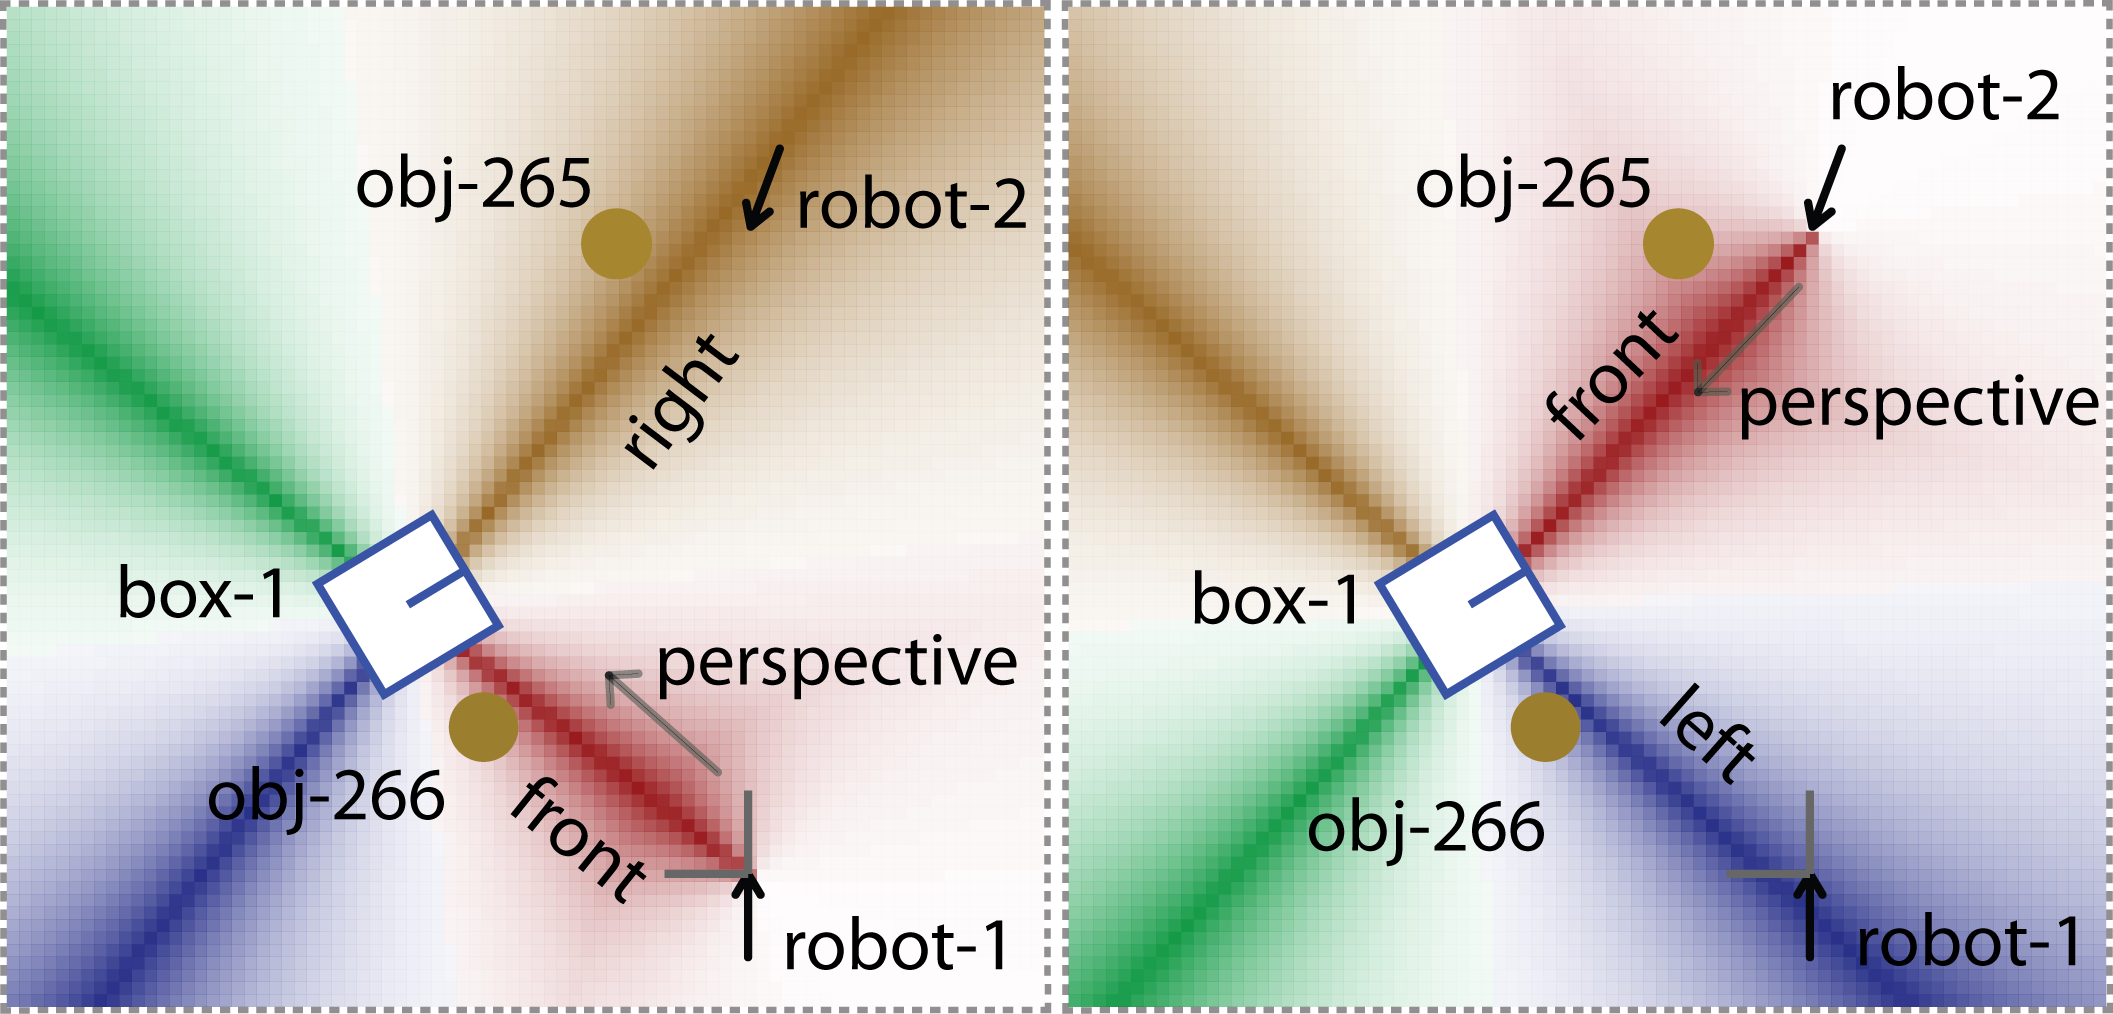
\includegraphics[width=0.7\columnwidth]{figs/space-scene-3-influence-perspective.png}
\caption[Influence of perspective on relative frames of reference.]
{The two figures show the influence perspective has on relative frames of reference.
The left figure shows the landmark {\footnotesize\tt box-1} when construed with a relative frame of reference
from the perspective of {\footnotesize\tt robot-1}. 
In this configuration object {\footnotesize\tt obj-266} is in front and object {\footnotesize\tt obj-265} is to the right.
Whereas when the same landmark {\footnotesize\tt box-1} is construed with a relative frame of reference
from the perspective of {\footnotesize\tt robot-2} it is object {\footnotesize\tt obj-265} which is in front,
whereas object {\footnotesize\tt obj-266} is to the left.}
\label{f:influence-perspective}
\end{center}
\end{figure}

The perspective of relative frames of reference is sometimes explicitly marked
by speakers. In the example \textit{der Block links von der Kiste von dir aus} (`the block left of the box from your perspective'),
the speaker choose to provide a perspective \textit{von dir aus} (`from your
perspective'). Only relative interpretations of a spatial phrase can be perspective 
marked. The perspective itself marks the position of the viewpoint, and therefore 
also the view direction, i.e. rotation. 

Intrinsic frames of reference computationally behave very similar to perspec\-tive-marked 
relative frames. Some argue therefore, that an intrinsic reference system is in essence a 
conflated relative reference system that coincides with the perspective 
on the scene \citep{levinson1996language}\oldindex{Levinson, S. C.}. 
Hence, intrinsic reference systems are never perspective marked, since they already 
include position and orientation. However, perspective marking is only compatible with relative 
frames of reference and excludes intrinsic the usage
of intrinsic or absolute frames of reference. 
On the other hand, relative reference systems always explicitly or implicitly mark 
perspective, since they cannot be conceived without since by definition relative 
reference systems always construe the world from a perspective (see
\figref{f:influence-perspective}).

Perspective on a scene is changed by an operation that transforms
a complete spatial context as if it had been perceived from a 
particular viewpoint.

\definition{Semantic operation}{geometric-transform}
\begin{explanation}{description}
Transforms the context to be viewed from a particular perspective.
Notice that perspectives require both a particular point of view
but also a rotation.
\end{explanation}
\begin{explanation}{arguments}
{\footnotesize\verb+?transformed-context+} (of type sensory-context) \\
{\footnotesize\verb+?context+} (of type sensory-context) \\
{\footnotesize\verb+?perspective+} (of type pose)
\vspace{0.3cm}
\end{explanation}

%%%%%%%%%%%%%%%%%%%%%%%%%%%%%%%%%%%%%
\section{Discussion}

\subsection{Functional constraints}\is{spatial relation!functional constraints}
Purely geometric accounts of spatial semantics have been criticized
on the basis of psycholinguistic studies that reveal for many spatial relations,
that additional functional constraints influence their applicability. 
Studies in particular for topological relations,
including \emph{in} and \emph{on}, but also for projective relations such as 
\emph{over} and \emph{under} \citep{coventry2001}\oldindex{Richards, L.}\oldindex{Prat-Sala, M.}\oldindex{Coventry, K.} as well as 
\emph{in front} and
\emph{behind} \citep{carlson1996influence}\oldindex{Carlson-Radvansky, L. A.}\oldindex{Radvansky, G. A.}  have led to new
proposals \citep{coventry2005spatial}\oldindex{Rajapakse, R.}\oldindex{Bacon, A.}\oldindex{Joyce, D.}\oldindex{Newstead, S.}\oldindex{Cangelosi, A.}\oldindex{Richards, L.}\oldindex{Coventry, K.} as to how to include functional
considerations into the semantics of spatial terms (see also 
\cite{coventry2004saying}\oldindex{Garrod, S.}\oldindex{Coventry, K.} for an overview). For instance, 
whether or not an umbrella is \emph{over} a person depends on 
the direction of rain which can come from different angles. 
I do not account for
functional constraints for two reasons: (1) because it requires detailed
functional models of objects which as of now are rarely available
in robots and (2) the current model theoretically can incorporate such models
once they become available. In order to acquire functional 
knowledge, such as that chairs 
are for sitting, tables are used to put things on and so forth, 
robots need to interact robustly and repeatedly with objects 
of this kind, in particular using complex 
interactions in which objects take on functional roles. Many of
these skills, e.g. basic actions such as sitting,
are contemporary research fields in robotics and still need to see 
significant progress before they are generally 
available. On the other hand, functional approaches to semantics
are typically committed to conceive the application of spatial
relations in terms of degree of applicability. In other words, 
functional models are essentially mappings of
locations and landmarks to some number representing the
degree in which some relation is deemed acceptable. This is 
precisely the basis of the semantics advocated in this chapter.
Semantic operations compute degrees of applicability. Consequently, 
once a functional model can be established in terms of similarity,
it can readily be incorporated into the current model by exchanging
semantic operations.

\subsection{Contextual factors}\is{spatial relation!contextual factors}
Besides functional constraints, contextual factors affect the
applicability of spatial terms. For instance, for proximal relations: 
\textsc{prototypical size} \citep{gapp1994basic}\oldindex{Gapp, K.}, but also 
\textsc{object salience} \citep{regier2001grounding}\oldindex{Regier, T.}\oldindex{Carlson, L. A.}, and \textsc{object interference} 
\citep{kelleher2009dialog}\oldindex{Costello, F. J.}\oldindex{Kelleher, J. D.} seem to play a role.
Just to give an example, the prototypical size factor can explain
why the proximal region \textit{nahe des Geb\"audes}
(`near the building') is larger than that of \textit{nahe dem Apfel} (`near the apple') 
(example adapted from \citealt{gapp1994basic}\oldindex{Gapp, K.}) by the difference in typical 
size of buildings and apples. 
Constraints such as the prototypical size, as well as the influence of
object salience, are easily integrated into the model, but just as 
for functional constraints do not affect the basic assumptions
of the model. The third constraint -- the object interference constraint --
refers to the interference by other objects that are for
instance closer than the related object. Such constraints are better treated 
under the problem of how to choose spatial relations which is inevitably
connected to the particular communicative goal. 
For instance, in a discrimination task other categories
might be more relevant for the task than in object location description tasks.
Such processes are dealt with in detail in \chapref{s:german-locative-phrases-semantic-processing}.


\subsection{Other modeling approaches}\is{spatial relation!spatial ontologies}\is{spatial relation!qualitative spatial reasoning}
Spatial semantics is an important and vibrant research area. 
Many different proposals are currently being made. Some suggest 
the use of formal ontology engineering \citep{bateman2007role,bateman2010situating,bateman2010ontology}\oldindex{Ross, R.}\oldindex{Farrar, S.}\oldindex{Bateman, J. A.}\oldindex{Hois, J.}\oldindex{Tenbrink, T.}
as a tool for enhancing spatial language interpretation by artificial 
systems. Others suggest to use formal reasoning techniques
and representations \citep{freksa1991qualitative,cohn2001qualitative}\oldindex{Hazarika, S. M.}\oldindex{Freksa, C.}\oldindex{Cohn, A. G.}.
The system presented in this book can benefit from these
extensive approaches in the sense that the detailed modeling 
of spatial representation and spatial reasoning could enhance
our modeling approach. On the other hand, in this book modeling 
serves the goal of establishing basic concepts, e.g. spatial relations,
so that we can later study their evolution. This is the
reason why more elaborate modeling approaches are avoided. Engineering
robust and extensive solutions for the processing of spatial
language is a valid goal in itself, but it is only one aspect of 
this book.

\subsection{Summary}
This chapter gave an account of the semantic core 
of German spatial relations in terms of geometric constraints,
frames of reference and perspective. Spatial relations have been
defined as graded categories, whose application is governed
by semantic operations. It remains to be shown (1) how 
conceptualizations of a scene given a concrete communicative
goal are achieved (a problem that can be summarized in how and 
which spatial relations should be chosen),  (2) how spatial
categorization fits into larger semantic structures for spatial
phrases such as \textit{der Block links von der Kiste} and (3)
how these semantics interact with language in production 
and parsing of spatial phrases.
 %\documentclass[a4paper,10pt,twoside]{diss}
%% \renewcommand{\includegraphics}[1][1]{} 
%\begin{document}

%%%%%%%%%%%%%%%%%%%%%%%%%%%%%%%%%%%%
\chapter{Syntactic processing}
\label{s:german-locative-phrases-syntax}
The syntax of German locative phrases mirrors the complexity of 
spatial semantics. The main task of syntactic processing is to 
allow agents to express themselves by translating semantic structure into 
proper German syntax and back. This chapter reports on the syntactic 
processing of German locative phrases using Fluid Construction Grammar. 
It provides an overview of the mapping from semantics to syntax and 
zooms in on different aspects of the implementation for dealing with complicated
syntactic phenomena such as the German case system.

Syntactic processing of German spatial language is primarily a problem
of orchestrating intertwined information processing. Great care
has to be taken to ensure that the ordered application of constructions 
in production and parsing of spatial utterances can proceed efficiently,without 
excessive branching in search. In many cases information
needed for processing is spread in the semantic structure to 
be produced or in the utterance to be parsed. For instance, 
lexical constructions might able to decide on word stems based
on semantic entities in the semantic structure, but already 
the decision which lexical class to use for expressing some lexical item 
in production requires a larger broader of the semantic
structure to be produced. Even more so, in order to decide on the actual
word form including German morphology, a whole array of syntactic information 
is to be considered. For instance, case, gender and number marking 
of spatial adjectives in prepositional noun phrases requires collection of  
information from the noun about its grammatical gender, and from 
the preposition about the required 
case. This chapter shows how advanced techniques
in FCG can be applied to organize efficient processing while 
allowing grammar designers to build extendable and concise grammars.

This chapter starts by presenting the general ideas behind the design of 
the grammar (\sectref{s:syntactic-processing-overview}) and
identifying core issues that have to be resolved in order to arrive at an
operational system. The remaining Sections \ref{s:lexical-functional}--\ref{s:handling-case} show how to deal with these issues.

\section{Overview of syntactic processing}
\label{s:syntactic-processing-overview}
One of the main problems of syntactic processing in a system that
is integrated with procedural semantics such as IRL is the problem
of how semantic structure such as IRL-networks are expressed
in language. The following are the two main ideas originally presented
in \citet{steels2005planning}\index{Steels, L.}\index{Bleys, J.}.
\begin{description}
\item[Lexicon] Lexical constructions directly map semantic entities 
to content words.
\item[Grammar] Grammatical constructions broadly speaking encode
the cognitive operations and the links between them and 
semantic entities. Consequently, grammar 
provides information on how semantic structure is combined \citep{steels2011phrasal}\index{Steels, L.}
by modulating the syntactic expression of the lexical items through
grammatical markers, word order, morphology, etc. 
\end{description}

German requires fine grained distinctions of constructions
in order to facilitate and coordinate processing. The grammar is 
organized into certain types of constructions each providing different information
(see \citealt{steels2011phrasal}\index{Steels, L.} for the original idea). 
\begin{description}
\item[Lexical Constructions] These constructions map semantic entities
to stems and back. Hand in hand with morphological constructions they
are responsible for the expression of lexical items. Lexical constructions
introduce lexical units in the transient structure\is{transient structure} that are used to assemble
information necessary for decisions on the lexical class and the word form 
of the semantic entity in production. In parsing these units gather information 
required for the semantic interpretation of a semantic entity in the 
surrounding semantic structure. Lexical constructions introduce abstractions
into the transient structure\is{transient structure} that allow to go from concrete semantic entities
to the class they are in. For instance, \textit{links} (`left') is a lateral spatial 
category such as \textit{rechts} (`right'). Both behave similar in semantics 
as well as in syntax. Lexical units introduce such type information
to allow hierarchy in processing to take advantage of this information.
\item[Functional Constructions] This class of constructions is related to
how a particular semantic entity is used in processing. For instance, in parsing,
when a spatial relation is observed as an adjective, this licenses the introduction 
of the cognitive operation {\footnotesize\tt apply-region-group-based} which represents how 
the spatial category is supposed to be applied. Consequently, functional constructions 
handle and process lexical classes and map them to particular cognitive operations.
These constructions introduce functional units into the transient structure, which
assemble all information related to lexical classes. On the semantic side
these units gather information related to the output and input of 
the cognitive operation. This information is particularly used by phrasal constructions
to combine functional units into larger phrases.
There are functional constructions for determiners, nouns, spatial adjective, spatial
adverbs and prepositions.
\item[Phrasal Constructions] These constructions, as the name suggests, are organizing both
larger syntactic structure, i.e. phrases, and larger semantic structure
by linking functional units. For instance in parsing, when observing
a spatial adjective and a noun in the correct German word order, the adjective-noun-phrase
construction links the processing of these items on the semantic side.
In turn, the new constituent can be further combined with determiners which
happens when the determined-noun-phrase construction applies.
Phrasal construction do the work of processing grammatical
relations between constituents. 
\item[Morphological Constructions] Certain constructions deal
exclusively with morphology. They are responsible for determining and 
processing word forms, i.e. the string, for expressing lexical items. In German
the concrete form of a lexical item is often determined by the larger
syntactic structure. For instance, a spatial adjective such as \textit{links} (`left') in
a determined adjective noun phrase has to agree with the gender and the number
of the noun and with the case of the determined noun phrase. This requires 
that in production the form of a lexical item is determined when this information
is available, which requires that constructions such as the determined-noun-phrase
construction have supplied this information. In parsing, morphological constructions
function as word form recognizers.
\item[Semantic Constructions] Lastly, there is a special type of constructions 
which is only used in parsing for handling semantic ambiguity\is{semantic ambiguity}. They are 
discussed in detail in \sectref{s:semantic-ambiguity}.
\end{description}

\begin{figure}
\begin{center}
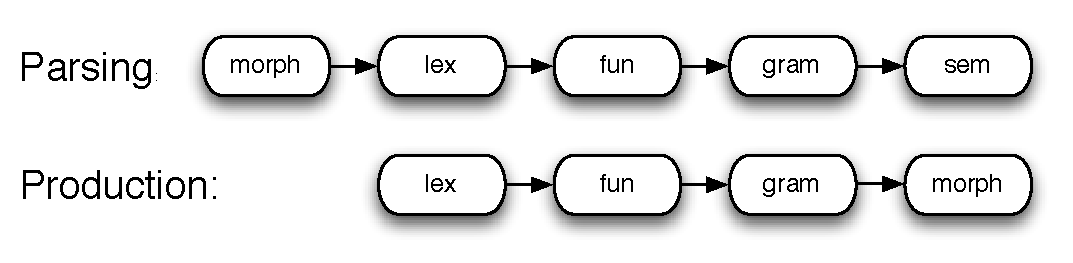
\includegraphics[width=.8\textwidth]{figs/cxn-application}
\end{center}
\caption[Construction application]{%
Construction application in the German spatial language 
grammar discussed in this chapter. In parsing,
morphological constructions apply first followed by lexical and 
grammatical constructions. Finally, the semantic constructions
important for handling semantic ambiguity apply. In 
production, these constructions are 
not applied. In contrast to parsing, morphological constructions apply in 
production at the very end in order to decide on the actual 
form used in the utterance.}
\label{f:construction-application}
\end{figure}

\figref{f:construction-application} shows the sequence of 
construction application in production and in parsing. 
In processing, the constructions are part of a 
large pool of constructions, which are applied based on which 
construction can apply at a specific point in time.
Syntactic processing proceeds bottom-up which means from the lexical 
items to the phrasal level. For instance, phrasal constructions require functional 
units to function which in turn depend on lexical constructions. In every
step information is assembled in hierarchical units, e.g. lexical units,
which expose new information, in order for constructions to use this information.
This process can also be understood as a process of gradual categorization
and assembly of constituents into larger structure both on 
the syntactic and on the semantic side. For instance, lexical constructions
abstract from the concrete semantic entity such as the spatial category 
{\footnotesize\tt left} and provide information about
the semantic type so that functional constructions can use this information
and apply to groups of spatial relations.

The following three sections look in more detail at the implementation
of different constructions such as lexical and functional 
(\sectref{s:lexical-functional}) phrasal constructions for landmarks
and landmark complements (\sectref{s:landmarks+complements})
and high-level phrasal constructions (\sectref{s:phrasal}).
The chapter concludes by discussing how to deal with the German
case system (\sectref{s:handling-case}).


\section{Lexical classes -- lexical and functional constructions}
\label{s:lexical-functional}
In German the same spatial relation can be expressed using different lexical classes
(adjective, adverb or preposition). The following shows 
an example of the spatial relation {\footnotesize\tt front} expressed
as adjective \REF{e:der-vordere-block-2}, adverb \REF{e:der-block-vorne-2}, 
and prepositions \REF{e:der-block-vor-der-kiste-2} which
are repeated here for convenience from \chapref{s:german-spatial-language-introduction}.
\ea
\label{e:der-vordere-block-2}
\gll der vordere Block\\
the.{\NOM} front.{\ADJ}.{\NOM} block.{\NOM}\\
\glt `The front block'\\

\z
\ea
\label{e:der-block-vorne-2}
\gll der Block vorne\\
the block.{\NOM} in the front.{\ADV} \\
\glt `The front block'\\

\z
\ea
\label{e:der-block-vor-der-kiste-2}
\gll der Block vor der Kiste \\
the.{\NOM} block.{\NOM} front.{\PREP} the.{\DAT} box.{\DAT} \\
\glt `The block in front of the box'\\

\z

Lexical classes are an example of a many-to-many mappings. 
Every German spatial relation discussed in this book
can be expressed in different lexical classes.
Vice versa, every lexical class has a number of relations that 
are part of it. For instance, the spatial relations {\footnotesize\tt front}, {\footnotesize\tt back}, 
{\footnotesize\tt left}, can all be expressed as adverb. 
However, not all spatial relations can
be expressed as adverbs. The proximal relations \textit{nah} (`near') and \textit{fern} (`far') 
do not occur in adverbial form.\footnote{Linguistic analysis is made 
difficult by diverging vocabulary in linguistics and different usages of 
the same term by different schools. I use the term adverb here for spatial relations
such as \textit{vorne} (`front') that can be followed by prepositional phrases and
used as postmodifiers on determined noun phrases e.g. 
\textit{der Block vorne in der Kiste} (`in the front area of the box').
\tabref{t:lexical-class-word-forms} gives an overview of lexical
classes and associated forms. The table shows that different
groups of spatial relations partake in different lexical classes. 
For instance, all spatial relations except for proximal relations 
such as {\footnotesize\tt near} and {\footnotesize\tt far} can be expressed as
adjectives. Projective relations such as {\footnotesize\tt up}, {\footnotesize\tt front}
and {\footnotesize\tt left} can be expressed as adverbs. Only
vertical and lateral relations can also be genitive prepositions, whereas
frontal relations can only be dative prepositions. Vertical relations can be both 
genitive and dative prepositions. 

\begin{table}
\label{t:lexical-class-word-forms}
\caption[Lexical Classes and word forms for German spatial relations]
{Lexical Classes and word forms for German spatial relations 
(adapted in part from \citealt{tenbrink2007space}\index{Tenbrink, T.}). This by no means
is an exhaustive list of spatial relations, lexical classes or lexical forms 
in German spatial language, but it is the part of German relevant for 
this book. Items marked with * seem to be possible, but due to being
unconfirmed in the reviewed literature are omitted.\newline}
\begin{tabular}{l>{\itshape}l>{\itshape}l>{\itshape}l>{\itshape}l}
\lsptoprule
Relation & \upshape Adjective & \upshape Adverb & \upshape Preposition [\textsc{poss}] & \upshape Preposition [\textsc{dat}] \\\midrule
{\footnotesize\tt up} & ober & oben & oberhalb & {\"u}ber \\%\hline
{\footnotesize\tt down} & unter & unten & unterhalb & unter\\%\hline
{\footnotesize\tt front} & vorder & vorne & \multicolumn{1}{c}{\upshape --} & vor \\%\hline
{\footnotesize\tt back}  & hinter & hinten  & \multicolumn{1}{c}{\upshape --} & hinter\\%\hline
{\footnotesize\tt right} & recht & rechts  & rechts & \multicolumn{1}{c}{\upshape --} \\%\hline
{\footnotesize\tt left} & link & links & links & \multicolumn{1}{c}{\upshape --} \\%\hline
% {\footnotesize\tt very-near} & &  & & an\\\hline
{\footnotesize\tt near} & \multicolumn{1}{c}{\upshape *} & \multicolumn{1}{c}{\upshape --} & \multicolumn{1}{c}{\upshape --} & nahe \\%\hline
{\footnotesize\tt far} & \multicolumn{1}{c}{\upshape *} & \multicolumn{1}{c}{\upshape --} & \multicolumn{1}{c}{\upshape --} & fern \\%\hline
{\footnotesize\tt north}  & n\"ordlich & \multicolumn{1}{c}{\upshape *} & \multicolumn{1}{c}{\upshape *} & n\"ordlich \\%\hline
{\footnotesize\tt south} & s\"udlich & \multicolumn{1}{c}{\upshape *} & \multicolumn{1}{c}{\upshape *} & s\"udlich \\%\hline
{\footnotesize\tt west} & westlich & \multicolumn{1}{c}{\upshape *} & \multicolumn{1}{c}{\upshape *} & westlich \\%\hline
{\footnotesize\tt east} & \"ostlich & \multicolumn{1}{c}{\upshape *} & \multicolumn{1}{c}{\upshape *} & \"ostlich \\%\hline
\lspbottomrule
\end{tabular}
\end{table}

The problem of choosing a lexical class in production and 
finding the lexical class in interpretation is solved by a careful
setup of the interaction of functional and lexical constructions.
I use a particular design pattern called \textsc{actual-potential}.\is{design pattern!actual-potential}%
\footnote{The pattern is inspired by earlier work on
argument realization \citep{vantrijp2008phd}\index{van Trijp, R.} which is 
also a many-to-many mapping problem.}
The design pattern allows to store possible lexical classes
in the form of potentials for each lexical item directly in the 
lexical units of the transient structure\is{transient structure}. Subsequent 
functional constructions can constrain their application based on the 
potential of the lexical item, consequently, ruling out 
non standard usage, e.g., expressing proximal relations as adjectives.
The same is used on the semantic side, where the semantic
type hierarchy of the semantic entity is stored as a list of potentials.

The actual-potential\is{design pattern!actual-potential} technique allows to 
distribute decision making across lexical and functional constructions 
by separating the specification of options (potentials)
from the \emph{actual} decision. Possible choices are
explicitly stored in the form of disjunctive potentials
in the transient structure 
thereby signaling to subsequent constructions which choices are 
possible which allows subsequent constructions to constrain their 
application by observing potentials and triggering only when
the right potentials are present. Before we jump to the 
application of the actual-potential\is{design pattern!actual-potential} design pattern, we need to 
consider the lexical and functional constructions that are involved.

The fact that Examples \REF{e:der-vordere-block-2}--\REF{e:der-block-vor-der-kiste-2} 
refer to the same projective category {\footnotesize\tt front} is expressed 
by the lexical construction for the spatial relation {\footnotesize\tt front}.
The construction maps the reference to the spatial relation onto 
the word stem \textit{vor}. The following template shows the lexical 
construction for the category {\footnotesize\tt front}:
\ea
\label{e:def-lex-front}
\begin{lstlisting}
(def-lex-cxn
 (def-lex-skeleton front-cxn 
  :meaning (== (bind frontal-category ?cat front)) 
  :args ((ref ?cat))
  :stem "vor"))
\end{lstlisting}
\z
Lexical constructions capture the similarity of different syntactic and
semantic usage scenarios of the same category. They encode
that no matter how the lexical item is used in the larger
semantic and syntactic structure it refers to the same
semantic entity, e.g. spatial relation.

Functional constructions map a particular lexical 
class to syntactic and semantic properties thereby
elevating lexical items to constituents in grammatical structure. 
On the semantic side, functional constructions trigger on semantic operations 
used in conceptualization. On the syntactic side, the constructions 
provide syntactic functions and syntactic classes in order for grammatical constructions 
to be able to build grammatical structure out of functional units.
Below are the skeletons for the functional constructions of spatial 
adjective, frontal adverbs and frontal prepositions:

\ea
\label{e:def-fun-spatial-adjective}
%\begin{footnotesize}
\begin{lstlisting}
(def-fun-cxn spatial-adjective 
 :meaning (== (apply-spatial-category-group-based 
                ?target ?source ?category))
 :args ((ref ?target)(src ?source)(cat ?category))
 :sem-function (modifier)
 :syn-function (adjectival))
\end{lstlisting}
%\end{footnotesize}
\z

\ea
\label{e:def-fun-frontal-adverb}
%\begin{footnotesize}
\begin{lstlisting}
(def-fun-cxn frontal-adverb 
 (def-fun-skeleton frontal-adverb
  :meaning (== (construct-region-frontal-internal
           ?target ?source ?landmark ?category ?f-o-r))
  :args ((ref ?target)(src ?source)
           (cat ?category)(landmark ?landmark))
  :sem-function (modifier)
  :sem-class (region internal-region relative-region)
  :syn-function (adverbial)
  :syn-class (adverb)))
\end{lstlisting}
%\end{footnotesize}
\z

\ea
\label{e:def-fun-frontal-preposition}
%\begin{footnotesize}
\begin{lstlisting}
(def-fun-cxn frontal-preposition
 (def-fun-skeleton frontal-preposition
  :meaning (== (construct-region-frontal 
             ?target ?source ?landmark ?category ?f-o-r))
  :args ((ref ?target)(src ?source)
           (cat ?category)(landmark ?landmark))
  :sem-class (angular-relationship)
  :syn-class (angular-preposition)))
\end{lstlisting}
%\end{footnotesize}
\z

These constructions introduce constructional meaning, e.g. 
{\footnotesize\tt construct-region-frontal}, together with semantic 
and syntactic potentials. One is the functional role of the
unit in the larger syntactic structure, here denoted by 
{\footnotesize\tt syn-function}. Aside from these two constructions, there are 
a number of other important functional constructions. 
In particular the difference in semantics of
lateral and frontal adverbs, but also between projective, topological
and absolute relations are each captured by separate 
functional constructions (see \tabref{t:functional-constructions} for an overview).


\begin{sidewaystable}
\begin{footnotesize}
\begin{tabularx}{\textwidth}{XXXXXXXXX}
\lsptoprule
name & lex-type & lex-cat & operation & sem-functions & sem-classes & syn-functions & syn-classes & examples 
% \\ \hline \hline
% color-adjective-cat  &color &color-adjective & apply-color-category &modifier & &adjectival & &gr\"un, rot 
\\ \midrule
spatial-adjective-cat  & spatial-category & spatial-adjective & apply-spatial-category-group-base &modifier & -- & adjectival & -- & \textit{linke}, \textit{rechte}, \textit{vordere}, \textit{hintere}
\\ \midrule
frontal-adverb  &frontal-category &frontal-adverb  & construct-region-frontal &modifier &relative-region, frontal-region, region &adverbial &frontal-adverb, adverb & \textit{vorne}, \textit{hinten} 
\\ \midrule
frontal-preposition  &frontal-category & frontal-preposition & construct-region-internal & -- & angular-relationship & -- & angular-preposition & \textit{vor}, \textit{hinter} 
\\ \midrule
spatial-preposition-cat  &spatial-category &spatial-preposition & construct-region-proximal &relationship & -- &preposition & -- & \textit{an}
\\ \midrule
lateral-adverb--preposition  &lateral-category &lateral-adverb--preposition & construct-region-lateral &modifier &relative-region, angular-relationship, ... &adverbial &lateral-adverb, angular-preposition, ... & \textit{links}, \textit{rechts}
\\ \midrule
noun-cat  &object-class &noun & apply-object-class &identifier & -- &nominal & -- & \textit{Block}, \textit{Kiste} 
% \\ \hline 
%pronoun-cat  &discourse-role & pronoun & identify-discourse-participant &reference & -- &referring-expression & -- &mir, dir 
\\ \midrule
article-cat  &selector &article & apply-selector &determiner & -- &determiner & -- & \textit{der}, \textit{die}, \textit{das} 
\\ \lspbottomrule
\end{tabularx}
\caption[Functional constructions]
{Overview of a subset of the functional constructions of the German grammar. 
The three columns {\footnotesize\tt lex-type},
{\footnotesize\tt lex-cat} and {\footnotesize\tt operation} show the requirements for each construction.
The four columns {\footnotesize\tt sem-functions}, {\footnotesize\tt sem-class}, {\footnotesize\tt syn-functions}
and {\footnotesize\tt syn-classes} detail the syntactic and semantic functions and classes that
the constructions introduce.}
\label{t:functional-constructions}
\end{footnotesize}
\end{sidewaystable}
%\begin{table}
%\begin{footnotesize}
%\renewcommand{\arraystretch}{1.5}
%\begin{tabularx}{\textwidth}{YYYYY}
%\lsptoprule
%\scshape name & \scshape lex-type & \scshape lex-cat & \scshape operation & \scshape sem-functions\\ \midrule
%spatial-adjective-cat  & spatial-category & spatial-adjective & apply-spatial-category-group-base & modifier\\
%frontal-adverb  &frontal-category &frontal-adverb  & construct-region-frontal &modifier \\%\midrule
%frontal-preposition &frontal-category & frontal-preposition & construct-region-internal & -- \\ %\midrule
%spatial-preposition-cat  &spatial-category &spatial-preposition & construct-region-proximal &relationship\\ %\midrule
%lateral-adverb--preposition  &lateral-category &lateral-adverb--preposition & construct-region-lateral &modifier\\ %\midrule
%noun-cat  &object-class &noun & apply-object-class &identifier\\ %\midrule
%article-cat  &selector &article & apply-selector &determiner\\ \midrule
%
%\end{tabularx}
%\begin{tabularx}{\textwidth}{YYYYY}
%	\scshape name &  \scshape sem-classes & \scshape syn-functions & \scshape syn-classes & \scshape examples \\ \midrule 
%	spatial-adjective-cat & -- & adjectival & -- & \textit{linke}, \textit{rechte}, \textit{vordere}, \textit{hintere}\\ %\midrule
%	frontal-adverb & relative-region, frontal-region, region & adverbial & frontal-adverb, adverb & \textit{vorne}, \textit{hinten}\\%\midrule
%	frontal-preposition & angular-relationship & -- & angular-preposition & \textit{vor}, \textit{hinter} 	\\ %\midrule
%	spatial-preposition-cat  & -- &preposition & -- & \textit{an}\\ %\midrule
%	lateral-adverb--preposition &adverbial &lateral-adverb, angular-preposition, ... & -- &\textit{links}, \textit{rechts} \\ %\midrule
%	noun-cat  & -- &nominal & -- & \textit{Block}, \textit{Kiste} 	\\% \midrule
%	article-cat & -- &determiner & -- & \textit{der}, \textit{die}, \textit{das} \\ \lspbottomrule
%\end{tabularx}
%\end{footnotesize}
%\caption[Functional constructions]
%{Overview of a subset of the functional constructions of the German grammar. 
%The three columns {\footnotesize\tt lex-type},
%{\footnotesize\tt lex-cat} and {\footnotesize\tt operation} show the requirements for each construction.
%The four columns {\footnotesize\tt sem-functions}, {\footnotesize\tt sem-class}, {\footnotesize\tt syn-functions}
%and {\footnotesize\tt syn-classes} detail the syntactic and semantic functions and classes that
%the constructions introduce.}
%\label{t:functional-constructions}
%\end{table}

\begin{figure}
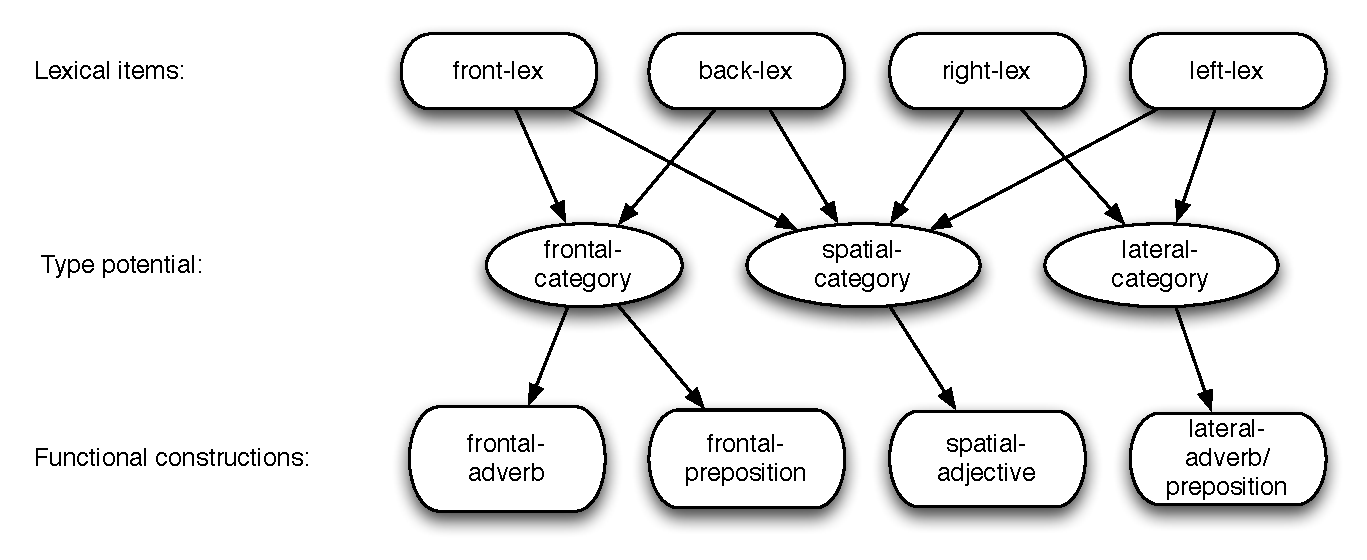
\includegraphics[width=\columnwidth]{figs/lexicals-type-potentials-cats}
\caption{Subset of the mapping of lexical items to functional constructions.}
\label{f:lexicals-type-potentials-cats}
\end{figure}

\subsection{Encoding type and lexical class potentials}
In order to solve the many-to-many mapping problem,
lexical and functional constructions are 
extended using the \emph{actual-potential}\is{design pattern!actual-potential} design pattern 
on the syntactic and semantic pole of constructions.
Lexical constructions merge semantic and 
syntactic potentials into lexical units. This 
information is used by functional constructions 
to constrain their application. On the 
semantic side, the {\footnotesize\tt type} constraints are rooted 
in the type hierarchy of spatial relations, whereas on the
syntactic side, the lexical class {lex-cat} potential encodes
which functional constructions can apply. 
The constraints take the form of disjunctive lists of potentials.
For example, since all angular categories, i.e. projective and absolute
categories, can be used as adjectives, the lexical constructions for these 
categories feature the {\footnotesize\tt type} potential {\footnotesize\tt angular-spatial-category}, 
as well as the syntactic {\footnotesize\tt lex-cat} potential 
{\footnotesize\tt spatial-adjective}. The adjective construction
constrains itself to only apply to lexical units that have this 
potential thereby licensing the application of the spatial adjective
construction. The lexical units for proximal relations, such
as {\footnotesize\tt near} and {\footnotesize\tt far} do not have these potentials, hence,
the adjective construction cannot apply.
Other fine-grained distinctions can be modeled as well.
Lateral and frontal projective categories differ in how their 
corresponding adverbs behave syntactically and semantically
which necessitates two functional constructions, one for lateral adverbs and one 
for frontal adverbs. Consequently, the potentials in frontal category units 
differ from lateral ones. They feature the type {\footnotesize\tt frontal-category}, 
where lateral lexical constructions (i.e. for {\footnotesize\tt left} and {\footnotesize\tt right})
provide the {\footnotesize\tt type} potential {\footnotesize\tt lateral-category}
(see \figref{f:lexicals-type-potentials-cats} 
for {\footnotesize\tt type}  potentials of projective lexical constructions and
\figref{f:lexicals-lex-cat-potentials-cats}  for {\footnotesize\tt lex-cat} potentials)

\begin{figure}
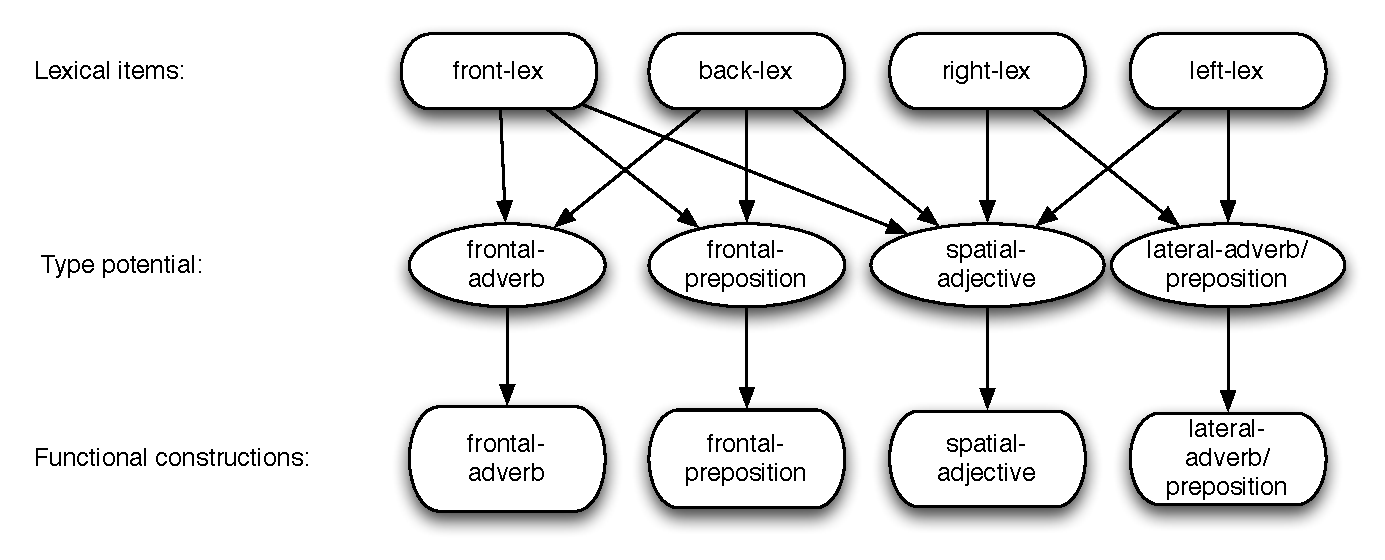
\includegraphics[width=\columnwidth]{figs/lexicals-lex-cat-potentials-cats}
\caption{Subset of the mapping from lexical items to functional constructions.}
\label{f:lexicals-lex-cat-potentials-cats}
\end{figure}

\subsection{Technical realization}
The actual-potential\is{design pattern!actual-potential} design pattern is easily implemented
using a dedicated template for extending lexical constructions.
Example \REF{e:def-lex-front}, for instance, is supplemented by the following two 
templates which introduce potentials on the semantic and syntactic side.
\ea
\label{e:def-lex-front-potentials}
\begin{lstlisting}
(def-add-potential front sem sem-cat type 
 (angular-spatial-category 
  projective-category 
  frontal-category))
(def-add-potential front syn syn-cat lex-cat 
 (spatial-adjective frontal-adverb frontal-preposition))
\end{lstlisting}
\z
These two templates specify the {\footnotesize\tt type} and 
{\footnotesize\tt lex-cat} potentials and directly translate into 
attributes in the {\footnotesize\tt front} lexical construction:
\ea
\label{e:def-lex-front-cxn}
\begin{lstlisting}
(...
 (J ?front-unit ?top ()
  ...
  (sem-cat 
   (== 
    (type 
     ((actual ?type-value)
      (potential 
       (angular-spatial-category 
        projective-category 
        frontal-category)))))
   ...)
...)
 <-->
(...
 (J ?front-unit ?top ()
  ...
  (syn-cat 
   (== 
    (lex-cat
     ((actual ?lex-cat-value)}
      (potential 
       (spatial-adjective 
        frontal-adverb 
        frontal-preposition))))
    ...))
...)
\end{lstlisting}
\z
Importantly, the template {\footnotesize\tt def-add-potential} 
not only adds the {\footnotesize\tt potential} attribute but also an 
attribute called {\footnotesize\tt actual}. This attribute, as we will
see in the next paragraphs, is automatically set to a variable 
in the lexical construction and is used to store which 
{\footnotesize\tt type} attribute is used. If one of the potentials 
is picked up, for instance by a functional construction, the 
{\footnotesize\tt actual} attribute is also set.

The information stored by the lexical construction in the transient structure\is{transient structure}
allows functional constructions to choose 
the potential in which they are interested and to constrain
their own application. This process can be seen in an extended 
version of the functional spatial adjective construction:
\ea
%\label{e:def-fun-spatial-adjective-potentials}
\begin{lstlisting}
(def-require-potential spatial-adjective 
  ?cat-unit sem sem-cat 
 type angular-spatial-category)
(def-require-potential spatial-adjective 
 ?cat-unit syn syn-cat
 lex-cat spatial-adjective)
\end{lstlisting}
\z
In order for the spatial adjective 
construction to apply, these templates express that certain potentials need to be present in the 
transient structure\is{transient structure}. More precisely, the {\footnotesize\tt type} potential 
{\footnotesize\tt angular-spatial-category} and the {\footnotesize\tt lex-cat} potential 
{\footnotesize\tt spatial-adjective} need to be there. 

The template for spatial adjectives translates into the following 
feature structure (for illustrative purposes, only the semantic 
side is shown here):
\ea
%\label{e:def-fun-spatial-adjective-potentials}
\begin{lstlisting}
(...
 (?cat-unit
  (sem-cat 
   (== 
    (type
     ((actual angular-spatial-category)
      (potential 
       (==! angular-spatial-category))))
    ...))
...)
\end{lstlisting}
\z
This construction can only apply if the {\footnotesize\tt type} potential 
of the lexical constituent in the transient structure imperatively includes 
{\footnotesize\tt angular-spatial-category}. Additionally,
it requires the {\footnotesize\tt actual} attribute
to be {\footnotesize\tt angular-spatial-category} or a variable. There are two
things to note here: the use of the {\footnotesize\verb|==!|} operator for 
potentials and the handling of the {\footnotesize\tt actual} attribute. 
The {\footnotesize\verb|==!|} operator only unifies and never merges, 
which means that neither in production nor parsing can a missing 
potential be merged. The specified potential always has to be present, 
in this case on the semantic side, but for the {\footnotesize\tt lex-cat} 
potentials, the case is vice versa on the 
syntactic side. Consequently, choosing a potential does not 
change the potential in the transient structure\is{transient structure}. 
The second feature, the {\footnotesize\tt actual} attribute, must be equal 
to {\footnotesize\tt angular-spatial-category} or a variable in order for the spatial 
adjective construction to apply. If the attribute
is a variable, then that variable is bound to {\footnotesize\tt angular-spatial-category}, 
and hence the application of the spatial adjective construction 
modifies the transient structure and sets the {\footnotesize\tt value} attribute 
to the required potential. Of course, the corresponding potential also 
has to be present for the construction to
apply in the first place (see \figref{f:production-vordere})

\begin{figure}
\begin{center}
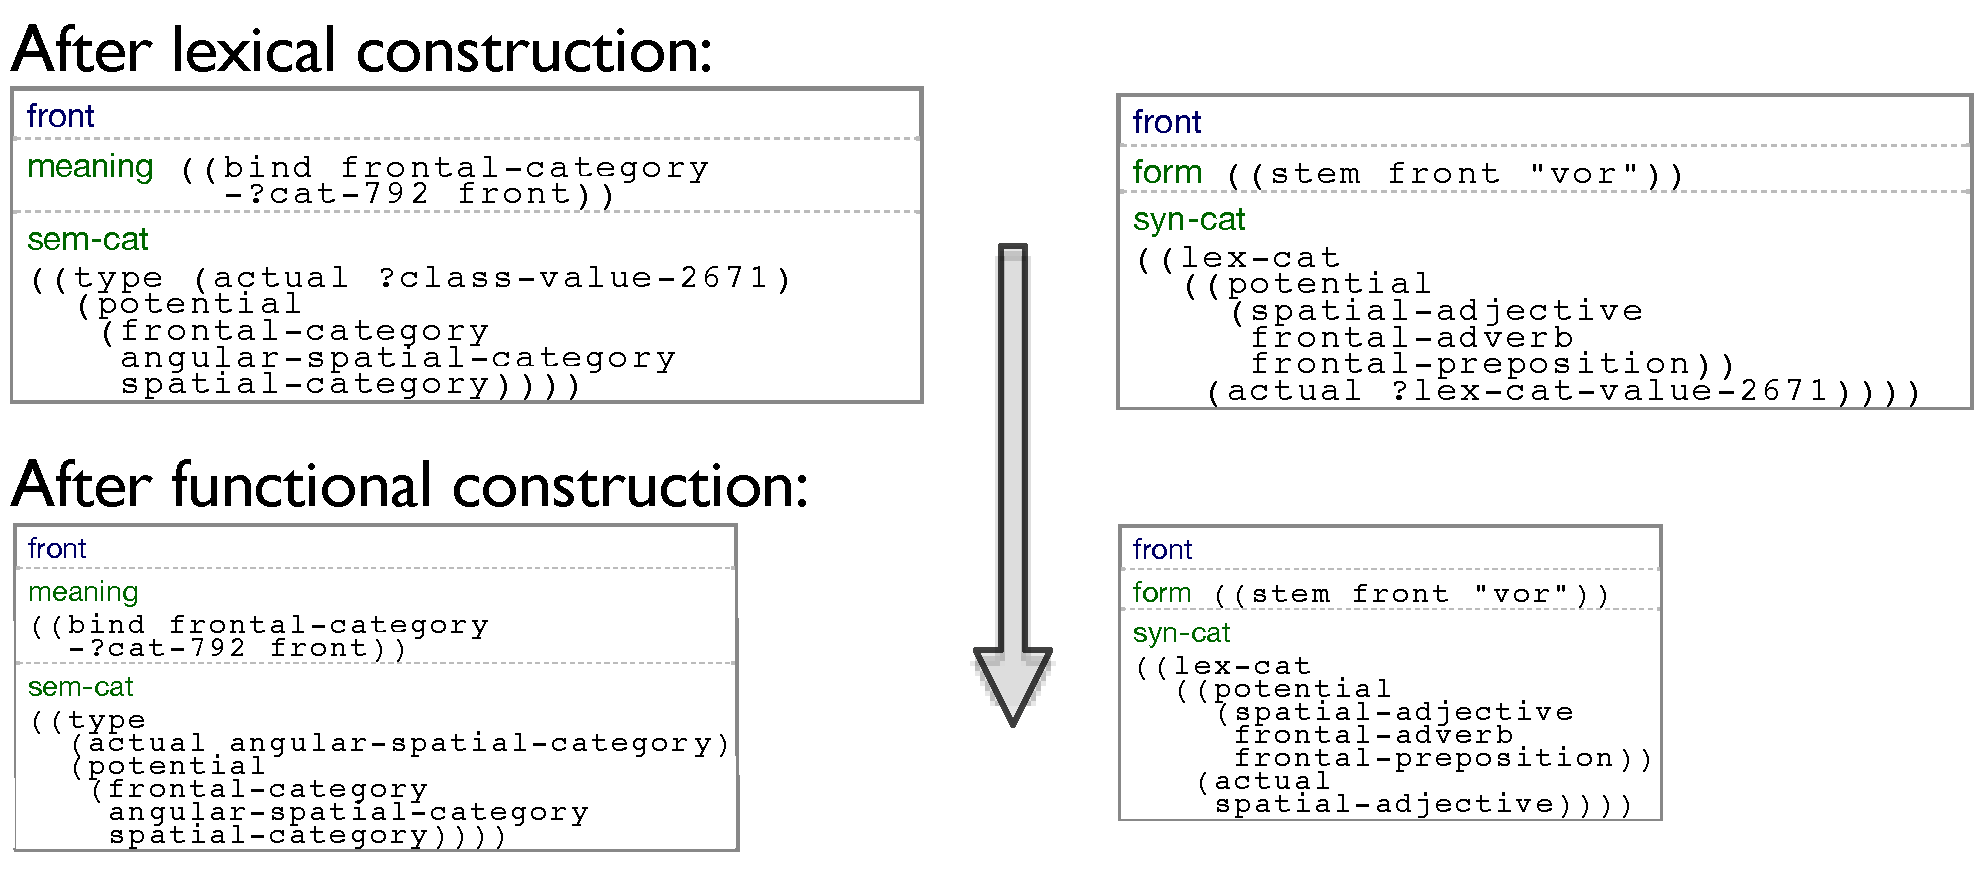
\includegraphics[width=.8\columnwidth]{figs/production-vordere}
\end{center}
\caption[Interaction of lexical and functional constructions -- syntax]{%
Interaction of lexical constructions with 
functional constructions in production of
\textit{vordere} (`front').
The arrow signifies the order of application. 
Left, the {\footnotesize\tt vordere} unit on the semantic side of the 
processed transient structure is shown. 
Right, the syntactic unit is shown. The 
transient structure\is{transient structure} actually contains more units, and the units 
themselves contain more features, but
everything has been shortened for illustrative purposes. The 
top row shows the lexical unit after
the application of lexical constructions, which have equipped 
the lexical unit with potentials
for {\footnotesize\tt type} on the semantic side, and {\footnotesize\tt lex-cat}  
on the syntactic side. Both of
these potentials have no value assigned to them yet. It is only 
after the application of the functional
construction of spatial adjective that both have values assigned 
to them, {\footnotesize\tt spatial-category}
for {\footnotesize\tt type} and {\footnotesize\tt spatial-adjective} for {\footnotesize\tt lex-cat}.}
\label{f:production-vordere}
\end{figure}

\begin{figure}
\begin{center}
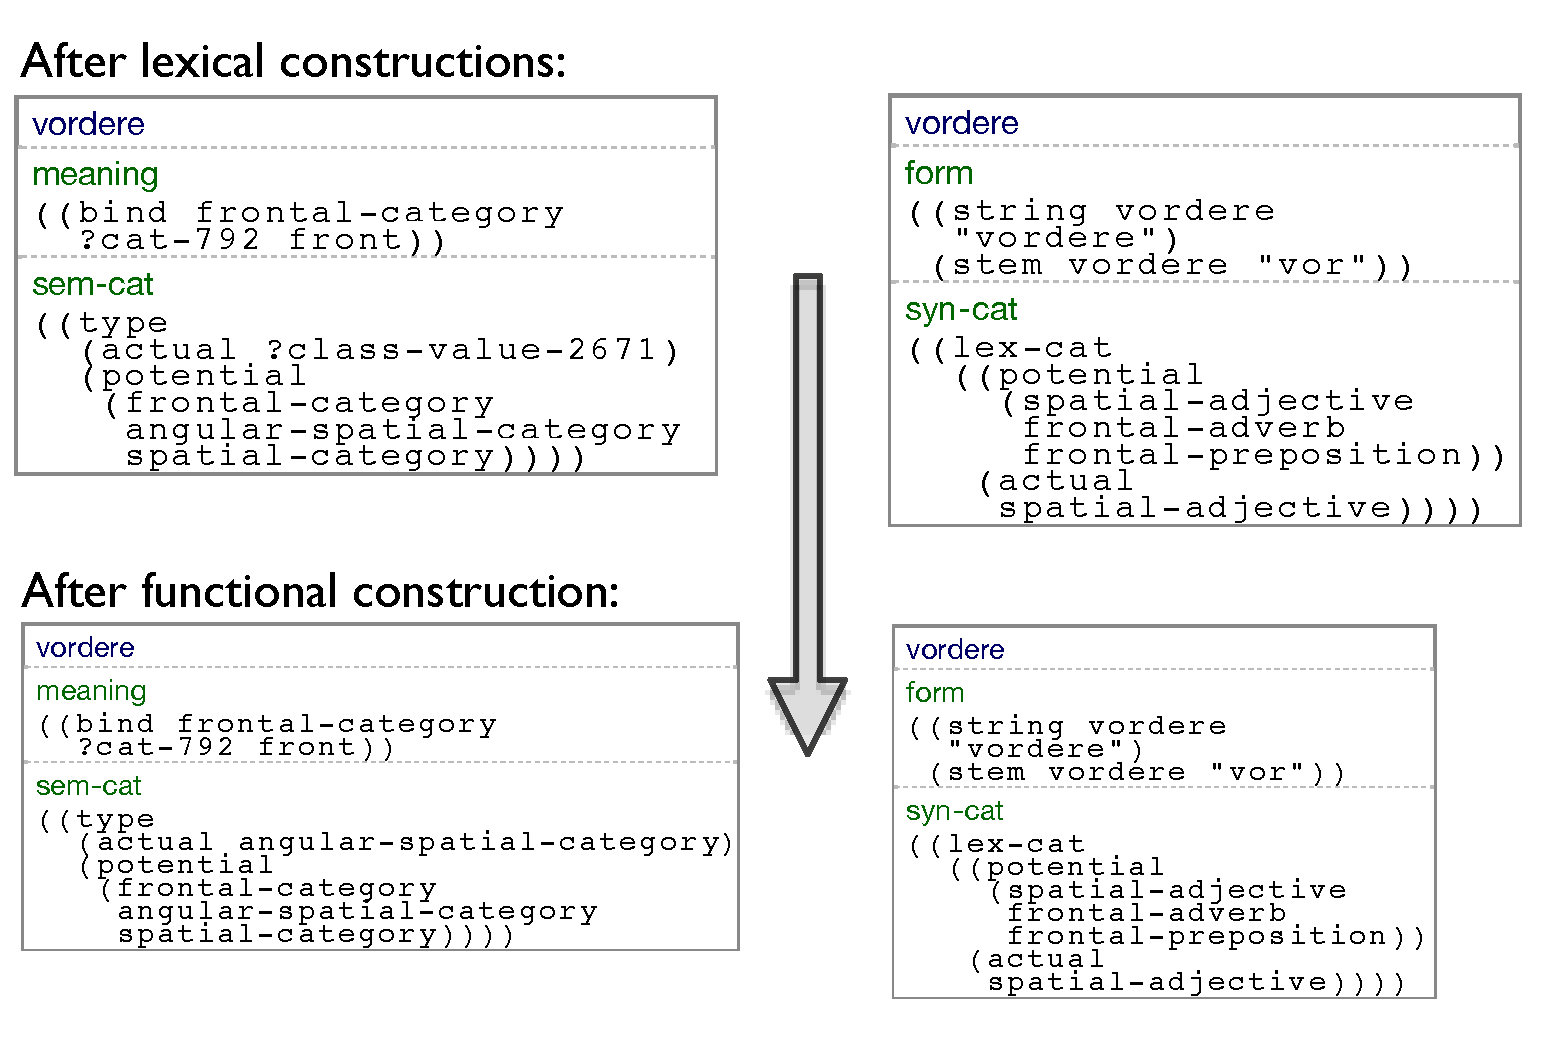
\includegraphics[width=.8\columnwidth]{figs/parsing-vordere}
\end{center}
\caption[Interaction of lexical constructions
with functional constructions -- semantics]{%
Interaction of lexical constructions 
with functional constructions in parsing \textit{vordere} (`front'). 
Lexical constructions apply before functional constructions.
The {\footnotesize\tt vordere} unit on the semantic side of the 
processed transient structure\is{transient structure} is shown on the left.
The syntactic unit is shown on the right. The transient 
structure actually contains more units, and the units themselves
contain more features, but everything has been shortened 
for illustrative purposes. The top row shows the lexical unit after the 
application of morphological and lexical constructions. The 
parsed string unambiguously allows for a decision to be 
made on the {\footnotesize\tt lex-cat} value, and 
hence the value is set on the syntactic side. It is the functional 
construction that picks one of the {\footnotesize\tt potential} {\footnotesize\tt types} 
on the semantic side and 
fills its {\footnotesize\tt value} attribute.}
\label{f:parsing-vordere}
\end{figure}

% explain interaction with morph rules 
This split into {\footnotesize\tt value} and {\footnotesize\tt potential} and 
the ability to interact via these two attributes is not only interesting
for grammar designers who can track the application
of constructions by tracing the actually chosen potential, but it also plays 
an active role in processing. In parsing,
the lexical class of a word is decided by morphological 
constructions. The morphological constructions apply first when 
parsing an utterance and they provide a value for the
{\footnotesize\tt actual} attribute. For instance, when observing the form 
\textit{vorne}, the morphological construction responsible for the
string \textit{vorne} triggers and adds the information to the transient 
structure, namely that an adverb was observed in parsing (see 
\figref{f:parsing-vordere} for a schematic overview).

\subsection{Discussion}
Handling the many-to-many mapping problem in lexical class choice
in principle also has other solutions. In particular, one could
rely on the search process of FCG in order to branch into all possible
lexical classes for a particular lexical item, and cut branches until only the 
one relevant for the current purpose, e.g. for the meaning produced, survives. 
This solution requires one lexical constructions for each possible lexical class
and for each category. This leads to excessive branching in search. 
The solution presented in this chapter does not require branching
in search and is thus more efficient. Another solution to this problem
is to code the interaction of lexical items and lexical classes in a holistic
fashion, which means that every possible combination of lexical class 
and lexical item is represented by exactly one construction. This 
solution does depend on branching of search, but demands grammar
designers to hand code many constructions (for the case discussed in
this chapter more than 30 combined constructions are needed). 
The solution presented in this chapter leads to a concise grammar,
with much fewer constructions (less than 20 lexical and functional constructions).


%%%%%%%%%%%%%%%%%%%%%%%%%%%%%%%%%%%%
\section{Landmarks and complements -- 
adverbial and prepositional constructions}
\label{s:landmarks+complements}
\chapref{s:german-spatial-language-introduction} contains a number of 
examples of landmark and perspective marking in German spatial 
phrases. Most importantly I concluded that in spatial prepositional phrases 
the landmark is always part of the prepositional phrase. This contrasts 
with adverbs which allow landmarks to be expressed optionally
using prepositional complements. Additionally, we have seen in
\chapref{s:german-space-semantics} how spatial semantics chiefly relies on particular 
semantic operations and linking of semantic structure. Consequently, 
there are two important questions related to processing landmarks and 
perspective in adverbial and prepositional phrases: (1) how to deal with 
optional elements in a concise way, and (2) how to achieve linking. 
In this section I explore the solution to these problems for projective categories, 
in particular projective adverbs and projective prepositions. 


\begin{sidewaystable}
\begin{footnotesize}
\begin{tabular}{p{1.6cm}p{1.6cm}p{1.6cm}p{1.6cm}p{1.6cm}p{1.4cm}p{1.4cm}p{3.5cm}}
\lsptoprule
cxn &  c1 syn-\newline function & c1 syn-class &  c2 syn-fn & c2 syn-class  & syn-functions & syn-classes & examples \\ \midrule
angular-pp-phrase & & angular-preposition & referring-expression & & adverbial & &[vor] [der Kiste], [links] [der Kiste]
\\ \hline  
lateral-region-landmark-marked  & adverbial &adverb & referring-expression & & adverbial & & [links] [von mir] 
\\ \hline  
relative-region-perspective-marked  &adverbial & &referring-expression & & & &
[vor der kiste] [von mir aus], [links] [von mir aus], [links von der Kiste] [von mir aus] 
\\ 
\hline
\hline
cxn name &  c1 sem-\newline function & c1 sem-class &  c2 sem-fn & c2 sem-class  & sem-functions & sem-classes & examples \\ \hline\hline
angular-pp-phrase & & angular-relationship & reference & & modifier & region, relative-region & [vor][der Kiste], [links][der Kiste]
\\ \hline
lateral-region-landmark-marked  & modifier & lateral-region & reference & & modifier & region, relative-region & [links] [von mir] 
\\ \hline
relative-region-perspective-marked  & modifier & relative-region &reference & &modifier & region &
[vor der Kiste] [von mir aus],[links] [von mir aus], [links von der Kiste] [von mir aus] 
\\ \lspbottomrule
\end{tabular}
\end{footnotesize}
\label{t:landmark-perspective-cxns}
\caption[Syntactic and semantic mappings of constructions]{%
Syntactic and semantic mappings of constructions 
governing prepositional and complemented adverbials. Syntactic and semantic
functions and classes for the two constituents ($c1$ and $c2$) are shown. To the right
the newly introduced syntactic and semantic function and classes are shown.}
\end{sidewaystable}

Let us first consider the extension of projective prepositions 
using a landmark. The construction handling projective and absolute 
prepositions is called {\footnotesize\tt angular-pp-phrase}. It has two constituents
(see \tabref{t:landmark-perspective-cxns}). 
The first constituent is one that has the semantic 
class {\footnotesize\tt angular-relationship} and the syntactic class 
{\footnotesize\tt angular-preposition} (see \tabref{t:functional-constructions} and in particular the semantic and 
syntactic function attributes of all projective 
prepositional constructions {\footnotesize\tt frontal-preposition},
{\footnotesize\tt lateral-preposition} and {\footnotesize\tt vertical-preposition})
functional construction). The second constituent is 
the landmark. For the landmark there are only functional constraints. 
Whatever is supposed to act as the landmark needs to be some kind of
{\footnotesize\tt reference} (semantic) and {\footnotesize\tt referring-expression} (syntactic). 
How is the linking precisely achieved? 
When we look at the prepositional construction in %Example 
\REF{e:def-fun-frontal-preposition}, we see that it features the variable 
{\footnotesize\tt ?landmark} connected to the landmark slot of the respective 
operation. Since FCG cannot rely on variable names as they 
might change, the variable is repeated in the {\footnotesize\tt args} feature, 
clearly marked in the attribute {\footnotesize\tt landmark}. 
This means that the {\footnotesize\tt angular-pp-phrase} construction
can unify with this specific argument, which is for this purpose. 
Let us look at the template to understand the linking.

\ea
\begin{lstlisting}
(def-phrasal-cxn angular-pp-phrase
 :constituents
 (def-constituent
  :syn-class angular-preposition 
  :sem-class angular-relationship
  :args ((landmark ?landmark)))
 (def-constituent
  :syn-function referring-expression
  :sem-function reference
  :args ((ref ?landmark)))
  :syn-function adverbial
  :sem-function modifier)
\end{lstlisting}
\label{e:angular-pp-phrase}
\z
Linking is achieved by explicitly unifying the corresponding 
{\footnotesize\tt args} in the structure, using the variable
{\footnotesize\tt ?landmark}. The variable occurs both in the {\footnotesize\tt ?ref} 
argument of the {\footnotesize\tt reference} constituent 
and the {\footnotesize\tt landmark} argument of the 
{\footnotesize\tt angular-relationship} constituents. 


For adverbs the linking with landmark works similar to prepositions. 
However, there are important differences in syntax between prepositions
and adverbs. Let us consider the example of lateral adverbs.
Lateral adverbs can be extended by landmarks, but the has to 
be marked using a \textit{von} prepositional phrase. 
The construction handling the landmark augmentation of lateral adverbs 
is shown below. In addition to linking, this construction introduces
the preposition \textit{von}. 


\ea
\begin{lstlisting}
%\begin{footnotesize}
%\begin{verbatim}
(def-phrasal-cxn lateral-adverb-landmark-marked
 :constituents
 (def-constituent
  :syn-function adverbial
  :syn-class lateral-adverb 
  :sem-function modifier
  :sem-class lateral-region
  :args ((landmark ?landmark)))
 (def-constituent
  :syn-function referring-expression
  :sem-function reference
  :args ((ref ?landmark))
  :preposition "von")
 :syn-function adverbial
 :sem-function modifier)
%\end{verbatim}
%\end{footnotesize}
\end{lstlisting}
\label{e:lateral-adverb-landmark-marked}
\z


These two constructions show how to solve parts of the  
complexity puzzle of the interaction of syntax and semantics, 
i.e. the linking issue, while at the same time they deal with the syntactic 
differences for adverbs (in this case only lateral adverbs are discussed, 
but similar constructions exist for vertical and frontal adverbs) and 
prepositions. Moreover, the two constructions also 
prevent frontal adverbs from being 
landmark-augmented by any of the two constructions, 
since frontal adverbs do not have
the {\footnotesize\tt angular-preposition} potential. Also they 
cannot be extended using the lateral 
landmark marking scheme, since they are not of class 
{\footnotesize\tt lateral-region}. Other constructions deal with 
\textit{in} prepositional phrases and frontal adverbs.

\begin{table}
%\begin{centering}
\begin{tabularx}{\textwidth}{>{\hsize=0.9\hsize}X>{\hsize=0.9\hsize}X>{\hsize=0.9\hsize}X>{\hsize=0.9\hsize}X>{\hsize=1.4\hsize}X}
\lsptoprule
cxn &  c1 syn-fn & c2 syn-fn & syn-fns & examples \\ \midrule
adjectival-nominal-phrase  &adjectival & nominal & nominal & [linke] [block] 
 \\ \hline  
determiner-nominal-phrase  &determiner & nominal & referring-expression & [der] [block] 
\\ \hline 
referring-expression-adverbial-phrase  &referring-expression & adverbial & referring-expression & [der block] [links], [der block]\newline [vor/an...] 
\\ \hline  
preposition-referring-expression-phrase  &preposition & referring-expression & adverbial & [an][der kiste] 
\\ \hline  
possessive  &referring-expression & referring-expression & referring-expression & [die linke Seite]\newline [der Kiste] 
\\ \lspbottomrule
\end{tabularx}
\caption[Mapping of syntactic functions]{Mapping of syntactic functions (phrasal constructions). All phrasal
constructions have two constituents and all build hierarchical structure by subsuming the two constituents (\emph{c1} and 
\emph{c2}) into a new unit. 
Columns \emph{c1 syn-fns} and \emph{c2 syn-fns} show the syntactic function potential expected from constituents.
The column \emph{syn-fns} details the syntactic function potential of the new unit. All constructions shown here
introduce word order and require the first constituent \emph{c1} to meet the second
constituent \emph{c2}, i.e. \emph{c1} has to be exactly before \emph{c2}.}
\label{t:phrasal-syn}

%\end{centering}
\end{table}

\section{Linking everything together -- high-level phrasal constructions}
\label{s:phrasal}
The previous section looked at prepositional and adverbial constructions. 
But there is more. Particularly, there are important constructions which only care 
about the syntactic and semantic functions of their constituents, and hence are 
widely applicable and underlie the ability of the grammar to build and parse 
complex recursive utterances involving many complemented phrases. Phrasal 
constructions have two constituents. The unification of constituents is based on 
the actual-potential\is{design pattern!actual-potential} design pattern. The constructions require their constituents 
to provide certain semantic and syntactic function potentials, while providing 
new potentials for semantic and syntactic functions themselves. 
All of them also introduce a particular word order and a particular linking 
of the arguments of their constituents and the meaning they express. They internally link
the arguments of constituents while providing new arguments themselves.
Hence, in production these constructions express particular linkings in the semantic structure using a particular word order. Vice versa, in parsing they introduce links in the semantic structure when observing a particular word order
of their functional constituents. 

The simplest example of such a construction is the {\footnotesize\tt adjectival-nominal-phrase}, which allows agents to build large adjective noun phrases 
(see \citealt{steels2011phrasal}\index{Steels, L.} for the original idea). 
Tables \ref{t:phrasal-syn} 
and \ref{t:phrasal-sem} detail the semantic and syntactic functions of 
the constituents of all phrasal constructions, as well as the syntactic 
and semantic function potentials they introduce. The adjectival 
nominal construction maps a constituent with syntactic 
function {\footnotesize\tt adjectival} and semantic function {\footnotesize\tt modifier} and a constituent with syntactic function nominal and semantic function identifier onto a new unit. Hence, it builds hierarchy by introducing a new unit with two subunits -- 
namely its two constituents. This new unit has the semantic function potential of identifier and the syntactic function 
potential nominal. There are a number of functional constructions providing such semantic and syntactic 
functions. Both color and spatial adjectives provide the semantic function {\footnotesize\tt modifier} and the syntactic
function {\footnotesize\tt adjectival}. The semantic function {\footnotesize\tt identifier} and the syntactic function {\footnotesize\tt nominal} are provided by nouns. Hence, when encountering such constituents in production, for instance because noun and adjective functional constructions have provided suitable constituents, the construction will form a new unit with semantic function 
nominal and introduce the German word order, where adjectives always come before the 
noun. This new structure can itself be considered functionally equal to nouns, as it features the same syntactic and 
semantic functions. It therefore can be subject to modification through other adjectives. Finally, units that have the
semantic function {\footnotesize\tt identifier} and the syntactic function {\footnotesize\tt nominal},
can be extended by determiners through application of the {\footnotesize\tt determiner-nominal-phrase}, which results in a unit that encapsulates the semantic function 
{\footnotesize\tt reference} and the syntactic function {\footnotesize\tt referring-expression} and
provides for all examples, where nouns or adjective modified nouns are determined
using an article.
\begin{table}
\begin{footnotesize}
\begin{tabularx}{\textwidth}{YYYYYY}
\lsptoprule
cxn &  c1 sem-fn & c2 sem-fn & sem-fns & operation  & examples\\
\midrule
adjectival-nominal-phrase  & modifier &identifier &identifier & &[linke] [block] 
\\ \midrule
determiner-nominal-phrase  & determiner & identifier & reference & & [der] [block] 
\\ \midrule
preposition-referring-expression-phrase & relation &reference & modifier &  & [an] [der kiste] 
\\ \midrule 
referring-expression-adverbial-phrase  & reference & modifier & reference & 
apply-region-filter & [der block] [links], [der block] [vor/an...] 
\\ \midrule 
possessive  & reference & reference & ref & possessive
& [die linke Seite] [der Kiste] 
\\\lspbottomrule
\end{tabularx}
\end{footnotesize}
\caption[Mapping of semantic functions]{Mapping of semantic functions of phrasal constructions. For every construction the semantic function 
potential that needs to be present for the two constituents \emph{c1} and \emph{c2} is shown, as well as the 
new semantic function potential provided (\emph{sem-fns}). Some of the constructions add additional meaning
with more complicated argument linking properties. All others however link the {\footnotesize\tt ref} argument of constituent two (\emph{c2}) to the {\footnotesize\tt source} argument of constituent one (\emph{c1}).}
\label{t:phrasal-sem}
\end{table}

This explains how adjectival noun phrases can be build, 
but how do adverbial complement phrases discussed in the 
previous section get linked to referring expressions? 
This is solved by {\footnotesize\tt referring-expression-adverbial-phrase}, 
which links constituents with the semantic/syntactic function 
{\footnotesize\tt reference/referring-expression} (example \textit{der Block} or \textit{der gr\"une Block}
and {\footnotesize\tt modifier/adverbial} (example \textit{links}, \textit{links von der Kiste}, 
\textit{vor der Kiste} \ldots) into a unit that not only syntactically introduces 
the word order, that the adverbial is behind the referring expression, 
but also links the meaning and adds the operation {\footnotesize\tt apply-region-filter}. 
This construction, besides linking meaning of constituents,
adds an operation that is applied to the output of the meaning 
of the adverbial phrase. Here, this operation is {\footnotesize\tt apply-region-filter}, which 
filters the context given a particular region. It is important to understand, 
that this particular construction can be so general only because 
all complements in the grammar compute regions. In other words all adverbial complements always denote a spatial region, be they prepositional phrases or adverbials or complemented adverbials. 
The {\footnotesize\tt referring-expression-adverbial-phrase} construction, that handles 
all adverbial complements of determined nominal phrases, only needs to care about 
modifiers and hence, its generality is based on the fact that semantically 
all adverbial complements in this grammar compute regions while observing 
a particular word order. If there would be other possible complements, this 
construction would also need to specialize on the semantic type of the constituents.

%%%%%%%%%%%%%%%%%%%%%%%%%%%%%%%%%%%%
%\section{Handling Semantic Ambiguity (on the Level of Grammar) -- Perspective Marking or Not?}
%\label{s:semantic-ambiguity}


%%%%%%%%%%%%%%%%%%%%%%%%%%%%%%%%%%%%
\section{Handling case}
\label{s:handling-case}
Case and gender agreement in German is an example of a 
highly distributed information
processing task. The constraints on these syntactic features 
are contributed by many different constructions 
and thus have to be incrementally integrated in order
to produce grammatical utterances in German. For instance, the
grammatical gender of a prepositional determined adjective noun phrase
is determined by the noun, as shown in the following example (\textit{Block}, masculine).
\ea
\label{e:hinter-dem-linken-block}
\gll hinter dem linken Block\\
behind.{\PREP} the.{\DAT} left.{\DAT} block.{\DAT}\\
\glt `behind the left block'\\
\z 
Alternatively, the case is governed by the preposition (\textit{hinter}, requires dative). The determiner (\textit{der}) and the
adjective (\textit{link}) have to be case and gender marked according to
the information provided from these different sources,
namely, both the determiner and adjective are used in
their masculine dative forms (\textit{dem} and \textit{linken}). In other words,
the concrete form of a projective adjective can only be fixed after
the complete syntactic structure is processed. Along the way, 
information about which
case to use (coming from the preposition) and about the gender (from the noun) need to be integrated. 
Consequently, the grammar needs to be set up such that sets of 
highly dependent constructions can interact for allowing a distributed  
decision on which forms to use when expressing a particular
meaning. This includes mechanisms for (1) representing the
state of information including its uncertainty, (2) moving information
around in order to facilitate decisions and spread their effect, and
(3) ways to postpone decisions until enough information is
accumulated. The solutions presented for these problems naturally
mirror the techniques discussed in the previous section. Logic
variables embedded in feature matrices\is{design pattern!feature matrix} are used to represent
uncertainty, percolation for moving information around and
constructions of a particular type in order to postpone decisions.

\subsection{Representing the state of information}
Distinctive feature matrices (see \citealt{vantrijp2011matrices}\index{van Trijp, R.}) are a means to
represent the current, possibly indecisive state of information in
processing. They allow different constructions to independently
contribute constraints on values of the syntactic, case and gender
features until enough information has been collected. Hence, feature
matrices function similarly to the logic variable used for
representing uncertainty in the previous section, as they are a
technique for accumulating information contributed by different
constructions. Distinctive feature matrices\is{design pattern!feature matrix} extend the concept of
logic variables and allow for the representation of dependencies between features
in processing.

The way lexical items interact with the case gender agreement system
is determined in part by the lexical item and in part by the word
class. Nouns, for instance, have a particular gender and always need to be marked for case,
which is governed by prepositions. Adjectives and articles
agree in case and number with the phrase in which they are embedded,
specifically with the noun. Consequently, the state of information for
some word classes is initially constrained. While adjectives and
articles have no constraints on case and gender, nouns already provide
information about their gender, and prepositions about the required
case. Distinctive feature matrices\is{design pattern!feature matrix} allow for the representation of such different
states of information in the transient structure\is{transient structure} in a unified way by
explicitly representing all combinations of possible feature values
in a matrix. For our German example, this information is captured in
a two dimensional matrix, where columns reflect the four German cases,
and rows reflect the three grammatical genders. Every field in the
matrix corresponds to a particular combination of case and gender,
such as accusative-masculine, and every field can either be explicitly
excluded (i.e. marked with a ``{\textminus}''), selected (i.e.  marked by a ``+'') or
in an unknown state of information, which is represented using
variables i.e. marked with a ``?'').

\begin{figure}[t]
  \centerline{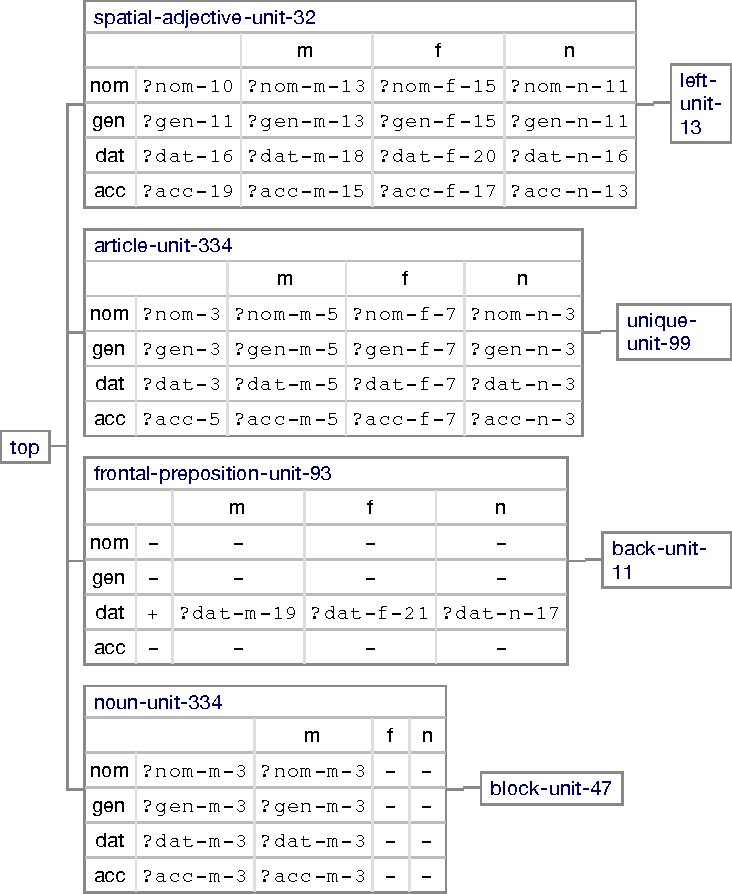
\includegraphics[scale=0.61]{figs/hinter-dem-linken-block-1}}
  \caption[Transient structure after the application of lexical and
    functional constructions]{Transient structure after the application of lexical and
    functional constructions for production of \textit{hinter dem linken
    Block} (`behind the left block'). For simplification, each unit
    is only shown with its distinctive feature matrix\is{design pattern!feature matrix} for case/gender
    agreement, if present. Furthermore, the feature matrices of the
    lexical units are identical to those of their parent units and are
    thus also not shown.}
  \label{f:hinter-dem-linken-block-1}
\end{figure}

\figref{f:hinter-dem-linken-block-1} shows the state of the
transient structure\is{transient structure} after the application of lexical and functional
constructions. It can be seen how the different states of information
for articles, adjectives, prepositions and nouns are technically
represented. The feature matrices\is{design pattern!feature matrix} for the spatial adjective
({\footnotesize\texttt{spatial-adjective-unit-334}}) and for the article
({\footnotesize\texttt{article-unit-334}}) are completely filled with variables. On
the other hand, the feature matrix\is{design pattern!feature matrix} for the frontal preposition
({\footnotesize\texttt{frontal-preposition-unit-93}}) features a ``{\textminus}'' everywhere but
in the column representing the dative case, namely, the case it
requires. On the other hand, the noun ({\footnotesize\texttt{noun-unit-334}}) is
categorized based on its gender, and the feature matrix\is{design pattern!feature matrix} consequently
has variables in the row for masculine and excludes all other fields.

\subsection{Percolation and agreement -- moving information around and unification}
Given the setup of initial information by lexical and functional
constructions, all subsequently applied constructions have to be able
to move information around and to further constrain the
information. Movement of information is done using percolation, and
unification of feature matrices for agreement automatically constrains
the values in the feature matrices further and further.

\begin{figure}[t]
  \centerline{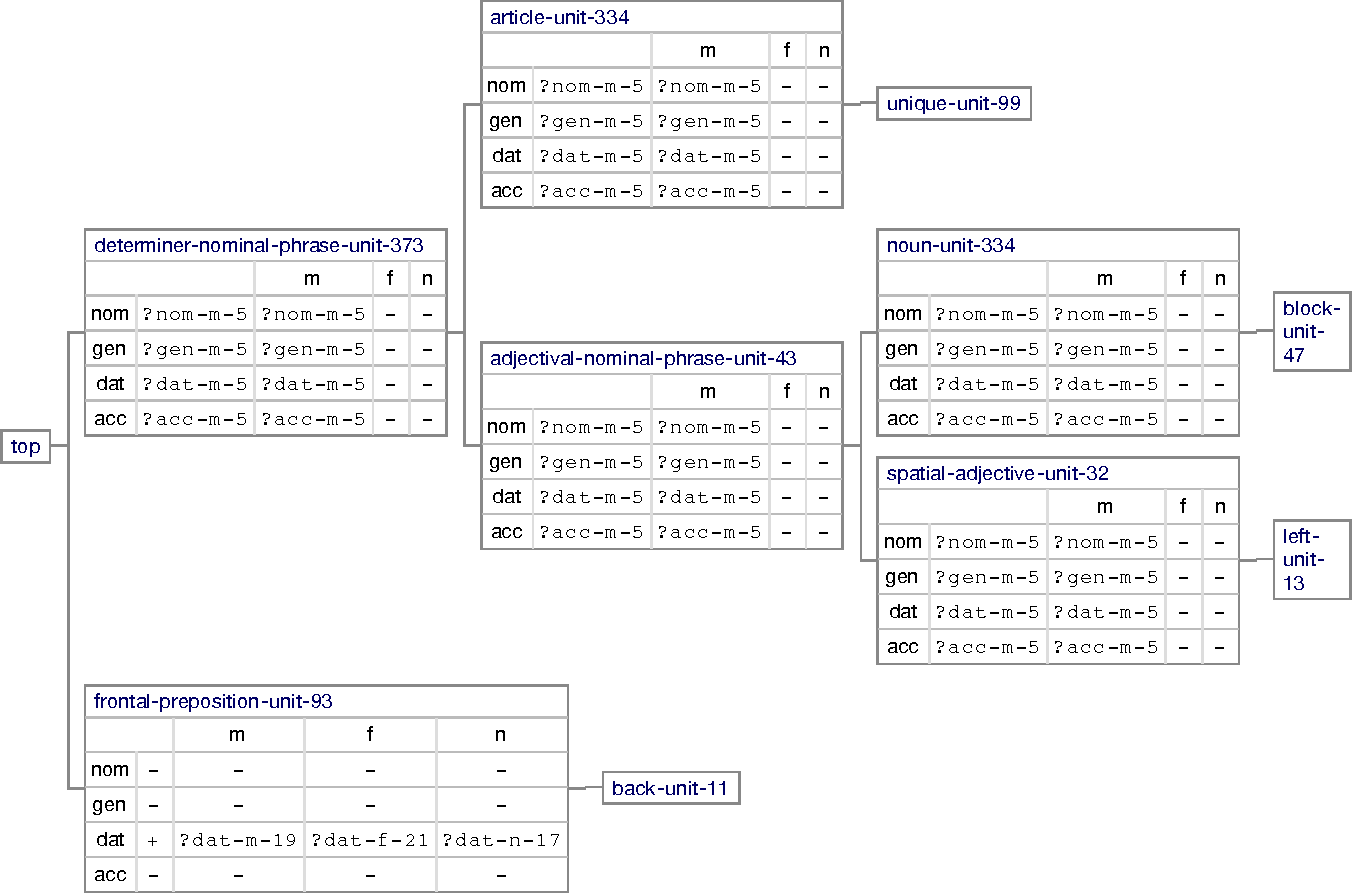
\includegraphics[scale=0.5]{figs/hinter-dem-linken-block-2}}
  \caption[Gender agreement represented in the transient structure]{%
  Gender agreement 
  between the article, adjective and noun
  are enforced by the adjectival-nominal and
  determiner-nominal-phrase constructions applied to the transient
  structure in Figure \ref{f:hinter-dem-linken-block-1}. }
  \label{f:hinter-dem-linken-block-2}
\end{figure}

Both percolation and unification are used together, for instance, by
the {\footnotesize\tt adjectival-nominal} construction (see Figure
\ref{f:hinter-dem-linken-block-2}). In our example, this construction
handles the adjective ({\footnotesize\texttt{spatial-adjective-unit-334}}) and
the noun ({\footnotesize\texttt{noun-unit-334}}) as constituents. Apart from introducing
German word order, this construction unifies the feature matrix\is{design pattern!feature matrix} of the
adjective and the noun, which automatically constrains the gender
possibilities for the adjective, in this case to masculine. In fact,
through unification the two feature matrices are the same after the
application of the {\footnotesize\tt adjectival-nominal}
constructions. Moreover, the newly created parent unit
({\footnotesize\texttt{adjectival-nominal-phrase-43}}) percolates this matrix
up. This process is subsequently repeated, this time by the
{\footnotesize\tt determiner-nominal} construction, which has the same effect
but this time with its constituents being the article and the
adjectival-nominal phrase, which also constrains the article to be
masculine. Percolation and unification have essentially
established the agreement between the article, the adjective and the
noun, while at the same time spreading the information about gender.


\begin{figure}[t]
  \centerline{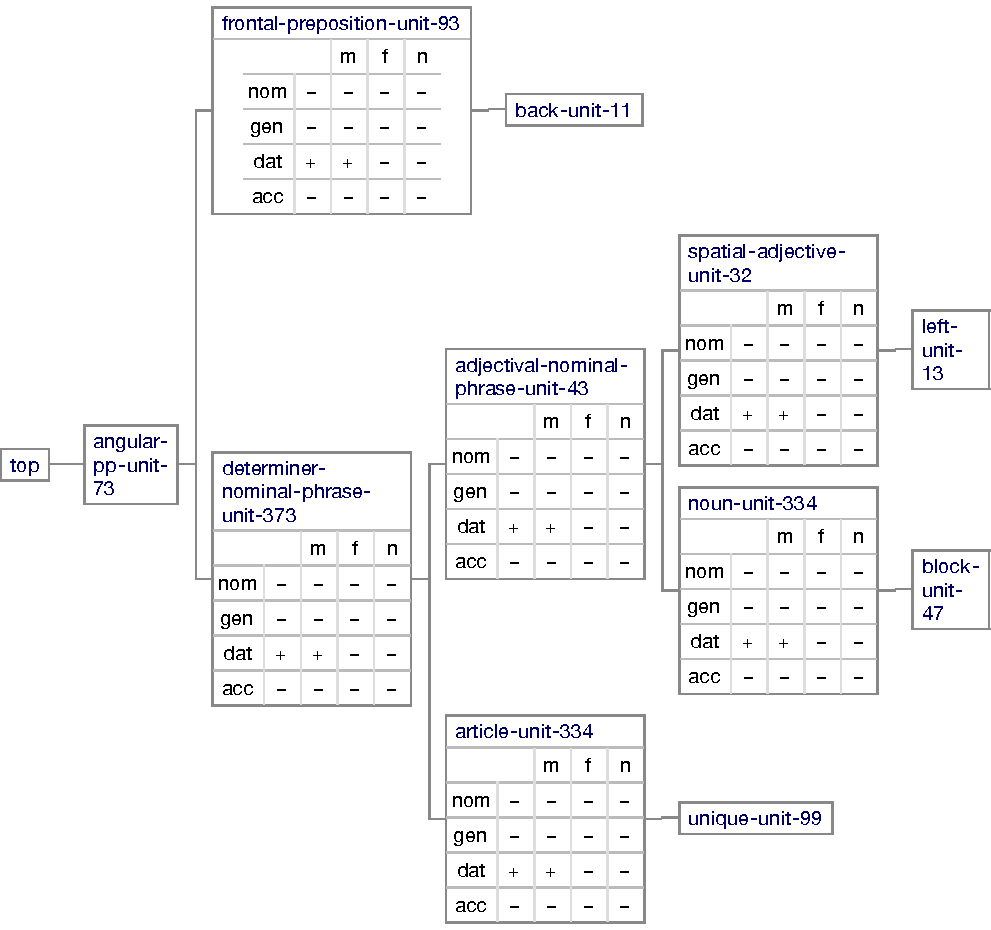
\includegraphics[scale=0.61]{figs/hinter-dem-linken-block-3}}
  \caption[Case agreement represented in the transient structure]{%
  Case agreement after applying the angular-pp-phrase
    construction to the transient structure from Figure
    \ref{f:hinter-dem-linken-block-2} while producing ``hinter dem
    linken block''.}
  \label{f:hinter-dem-linken-block-3}
\end{figure}


After the application of these two constructions, the decision on case
is still missing. Case is provided by the angular preposition, and
agreement between the preposition and the determined-nominal-phrase is
established by the {\footnotesize\tt angular-pp-phrase} (see \figref{f:hinter-dem-linken-block-3}). The {\footnotesize\tt angular-pp-phrase}
technically behaves very similarly to the the {\footnotesize\tt determiner-nominal} and the {\footnotesize\tt adjectival-nominal}
constructions: it unifies the feature matrices\is{design pattern!feature matrix} of its two constituents
({\footnotesize\texttt{frontal-preposition-unit-93}} and
{\footnotesize\texttt{determiner-nominal-phrase-unit-373}}). However, the effect is
quite different in that now the feature matrix of the article, the
adjective and the noun is further constrained in terms of
case. Consequently, case and gender of this particular phrase are
ultimately decided.

\begin{figure}[t]
  \centerline{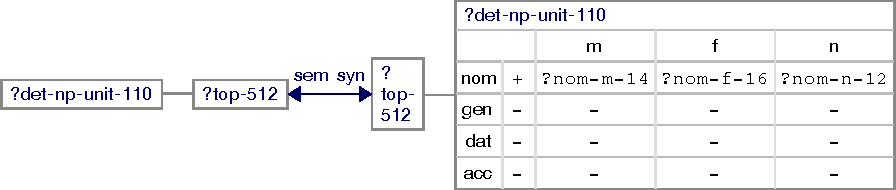
\includegraphics[scale=0.65]{figs/referring-expression-fvm}}
  \caption[Handling case in single determined-noun-phrases]{%
  The referring-expression construction sets the case of a
    single determined-noun-phrase unit to nominative.}
  \label{f:referring-expression-fvm}
\end{figure}

For some phrases case is not established by prepositions but
rather by the general grammatical structure. A prime example is when 
the utterance itself only consists of a noun phrase, which then needs to be marked by 
the nominative case. For example when meanings for utterances such as \textit{der
linke Block} (`the block to the left') are expressed, then there
is no preposition that determines the case of the whole
phrase by agreement. Rather, the {\footnotesize\texttt{referring-expression}}
construction (see \figref{f:referring-expression-fvm})
introduces the nominative case by unifying the feature matrix\is{design pattern!feature matrix} of the
determined-noun-phrase unit with a matrix constraining the case to
nominative.

\subsection{Postponing decisions}
After the application of the {\footnotesize\tt angular-pp-phrase}
construction, all necessary information has been accumulated. Case and
gender are decided, and hence all syntactic features for the
particular word class in question are available to allow subsequent
constructions to be able to decide the word form to be used. Morphological
constructions are used here to represent this relationship between syntactic
features and word forms. For example, for determiners there
are six different articles in German that unevenly cover the 12
possible case-gender combinations, as shown in the chart below:

\begin{center}
  \begin{tabular}{cccc}
  	\lsptoprule
    & m & f & n \\ \midrule
    nom  & \emph{der} & \emph{die} & \emph{das} \\
    gen  & \emph{des} & \emph{der} & \emph{des} \\
    dat & \bf{\emph{dem}} & \emph{der} & \bf{\emph{dem}} \\
    acc & \emph{den} & \emph{die} & \emph{das} \\ 
	\lspbottomrule
  \end{tabular}
\end{center}

\begin{figure}[t]
  \centerline{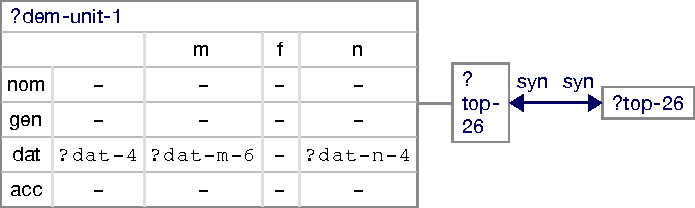
\includegraphics[scale=0.65]{figs/dem-morph-fvm}}
  \caption[Distinctive feature matrix\is{design pattern!feature matrix} of a morphological construction]{%
  Distinctive feature matrix of the morphological construction
    that maps the string \textit{dem} to masculine or neuter and dative
    articles. Note that since this is a morphological construction, both
    poles of the construction apply to the syntactic pole of a transient
    structure.}
  \label{f:dem-morph}
\end{figure}

For each of these forms, a separate morphological construction exists
which decides on the form used to express the article
based on the lexical class and the case-gender feature matrix. An example of such a
morphological construction is shown in Figure \ref{f:dem-morph}. Since
this construction has a variable in the dative masculine field, it
matches with unit {\footnotesize\texttt{unique-unit-99}} in Figure
\ref{f:hinter-dem-linken-block-3}. Similarly, other morphological
entries add the strings \textit{linken} to the {\footnotesize\texttt{block-unit-47}},
\textit{Block} to the {\footnotesize\texttt{block-unit-47}} and \textit{hinter} to
{\footnotesize\texttt{back-unit-11}}.

%%%%%%%%%%%%%%%%%%%%%%%%%%%%%%%%%%%%
\begin{figure}
\begin{centering}
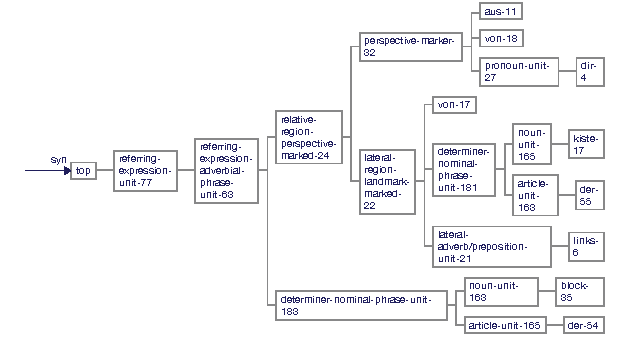
\includegraphics[width=\columnwidth]{figs/parse-result-transient-syn}
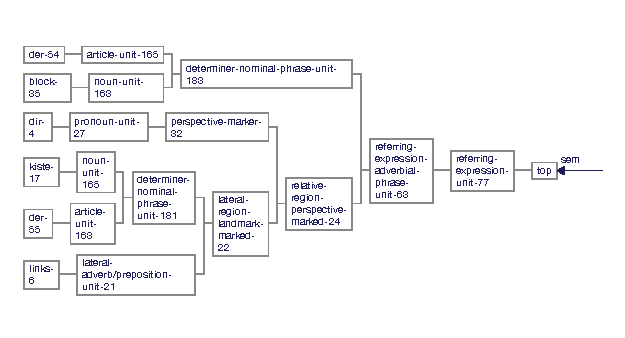
\includegraphics[width=\columnwidth]{figs/parse-result-transient-sem}
\caption[Final transient structure]{Parts of a final transient structure\is{transient structure}. The top shows the syntactic pole. The bottom
shows the semantic pole.}
\end{centering}
\label{f:parse-result-transient}
\end{figure}
\section{Summary}
Problems of intertwined information processing across multiple constructions 
and across different parts of transient structures often appear when dealing 
with complex, real world language. This chapter detailed how to tackle such 
problems using (1) adequate information representation techniques, such 
as logic variables, feature matrices\is{design pattern!feature matrix} and disjunctive potentials,
(2) percolation for distributing information in the transient structure, and 
(3) special constructions which are needed to help postpone decisions until 
the state of information is ready. The techniques have proven to be 
sufficient for handling problems of syntactic indeterminacy, e.g.
morphology and lexical class choice in German locative phrases. 
The discussed design patterns allow grammar 
designers to spread information processing across many constructions, 
leading to concise grammars, while facilitating efficient processing. 

The grammar is powerful enough to deal with German locative
phrases that include spatial relations, landmarks and even perspective.
\figref{f:parse-result-transient} shows the final transient structure when an agent
parses the phrase \textit{der Block links von der Kiste von dir aus} (`the block
to the left of the box from your perspective').

%\bibliographystyle{diss}
%\bibliography{papers,space} 
%\end{document}
 % \documentclass[a4paper, 9pt, fleqn]{diss}
% \include{format-and-defs}
% \begin{document}

%%%%%%%%%%%%%%%%%%%%%%%%%%%%%%%%%%%%
\chapter{Semantic processing}
\label{s:german-locative-phrases-semantic-processing}

In previous sections, I concentrated on how to represent the semantics
of spatial relations. In this section I focus on how to conceptualize, 
i.e. how to choose a particular spatial relation, frame of 
reference, landmark or perspective in order to refer to some object
in the environment. This chapter gives an overview of the factors
influencing conceptualization (\sectref{s:factors-of-conceptualization}),
followed by details of how conceptualization for spatial scenes can
be implemented (\sectref{sec:8.2}). Lastly, I compare the approach favored in this
book to another approach often used in modeling 
(\sectref{s:categorization+discrimination}). This last 
section also looks at the performance of the conceptualization
machinery presented in this chapter.


\section{Factors influencing semantic processing}
\label{s:factors-of-conceptualization}
A number of factors influencing the particular
choice in a particular context have been identified by scholars. 
First, the communicative intention of the speaker plays a major role. 
Whether the speaker wants to describe the spatial position of an 
object or discriminate it with respect to other objects in the context or whether
he is trying to give a route description \citep{tversky1998space}\index{Tversky, B.}\index{Lee, P.},
impacts on which spatial relations agents choose to express.
Second, the context and in particular the presence and position of landmarks,
their affordances with respect to frames of reference, the presence
of geocentric reference systems and the perspective of the interlocutor 
all influence the choices agents make.
Third, the available repertoire of spatial relations, frames of reference,
as well as cultural factors are no less important. For instance, in some cultures 
social status governs the choice of perspective.
How to talk about an object, in other words, how to conceptualize
the world for reaching the particular communicative goal
technically requires agents to choose semantic structure, 
including semantic operations and categories. 
Since we understand semantic structure as a program, the process 
of choosing appropriate semantic structure is essentially one of 
automatic programming, in which programs are constructed and 
tested based on their fitness for the particular task. 
The fitness or utility of some automatically constructed semantic structure 
is decided based on (1) the current communicative goal, e.g. to discriminate an object, 
(2) current spatial setup, in particular the position of objects,
(3) available categories and concepts.


\begin{figure}
\begin{centering}
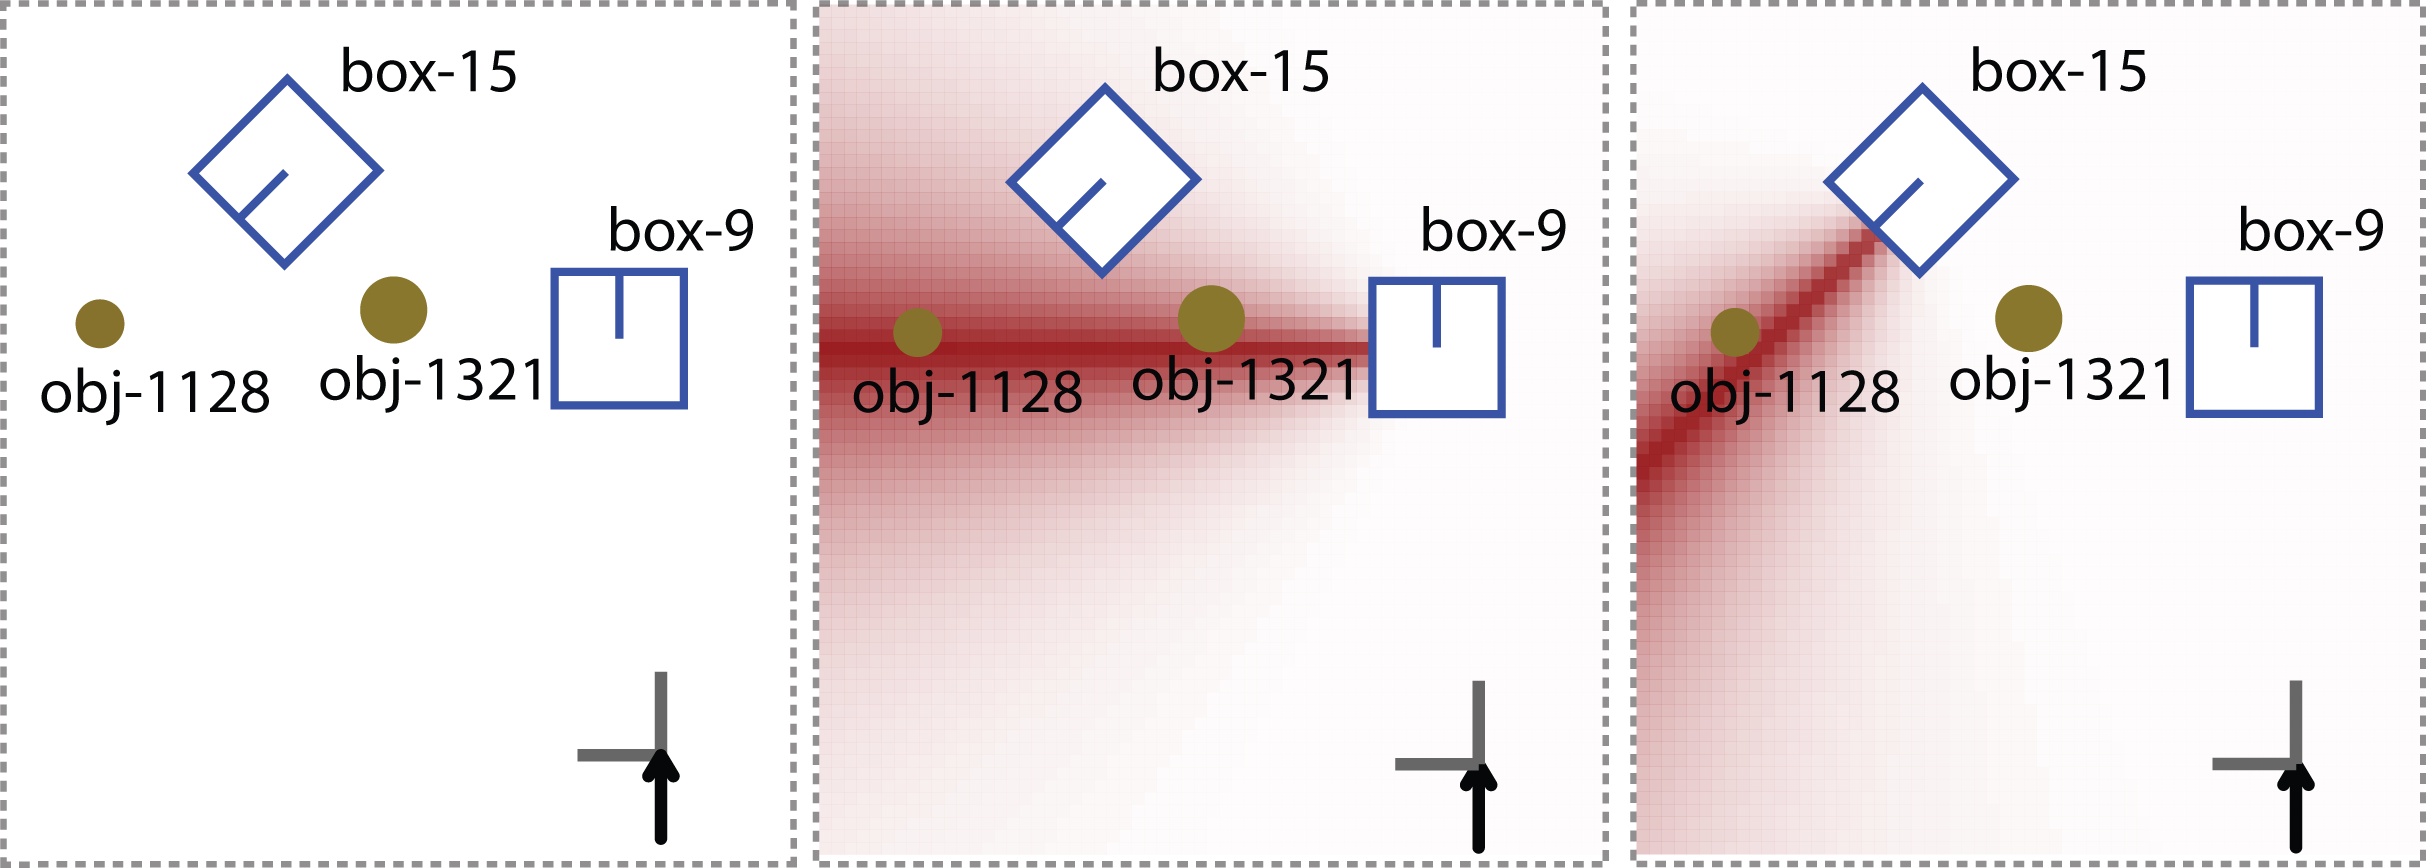
\includegraphics[width=.8\columnwidth]{figs/description-vs-discrimination.png}
\end{centering}
\caption[Difference between discrimination and description]
{Difference between description and discrimination. The left figure
shows the original context. The middle picture shows that
object {\footnotesize\tt obj-1128} lies in the region described by ``left of box-9'' 
(intrinsic reading) with a high score. However, object {\footnotesize\tt obj-1321}
lies pretty much in the same region of high applicability. In other words,
``left of box-9'' is not discriminating. The right figure shows an example of
a discriminating spatial relation. ``In front of box-15'' (intrinsic reading) 
clearly discriminates object {\footnotesize\tt obj-1128} from {\footnotesize\tt obj-1321},
as the score of both objects for this description varies significantly.}
\label{f:discrimination-vs-description}
\end{figure}

% communicative goal
\subsection{Influence of type of communicative goal -- which vs where}
Which communicative goal an agent is pursuing is an important 
driving factor in how he will conceptualize the world for reaching 
that goal. But it is not only the particular object an agent wants to talk 
about that makes a difference, but also the agent's intentions with 
respect to the object. For instance, there are important differences 
between descriptive and discriminating utterances. 
In discrimination scenarios, in answers to questions 
of the form \textit{Welcher?} (`which') the hearer is required to distinguish, in 
other words identify, an object. This relies chiefly on the overall 
spatial setup including the position of other objects 
in the scene. \textit{Wo?} (`where') questions, e.g. \textit{Wo ist der Block?} (`where is the block'),  
on the other hand are asking for descriptions of the spatial relations an object takes 
part in. In psychological experiments
spatial descriptions are elicited using contexts with only a 
single object \citep{levinson2003space}\index{Levinson, S. C.}. 
In description scenarios the applicability
of a spatial relation is the important aspect, 
whereas in discrimination scenarios, the power to contrast the
target object from the rest of the objects is more important 
(\citealt{tenbrink2005identifying}\index{Tenbrink, T.}, see \figref{f:discrimination-vs-description} for an example). 
Agents in discrimination scenarios choose spatial relations and
reference systems based on maximizing the distance to other objects
\citep{herskovits1986language}\index{Herskovits, A.}.

\subsection{Influence of spatial contexts}
Naturally, the spatial position of objects in the context has a
direct effect on which spatial relations might be applicable for
discriminating an object. This is based on
the discussion of discrimination in the previous paragraph, 
but it also holds, somewhat trivially, because the position of an 
object with respect to another object determines the applicability 
of a spatial relation between the two. But there are of course other factors
related to context that need to be taken into account.
Examples are the presence or absence of landmarks for construing the world
in relation to them and the availability of geocentric
features which allow for the application of absolute frames of 
reference. Furthermore, landmarks without intrinsic features, such 
as trees who have no inherent front, 
prevent the application of intrinsic frames of reference, and lastly, available perspectives on a scene influence the layout
of relative frames of reference on landmarks. In other words,
the particular spatial setup has an effect on the 
space of possible or even desirable conceptualizations.

\begin{figure}
\begin{centering}
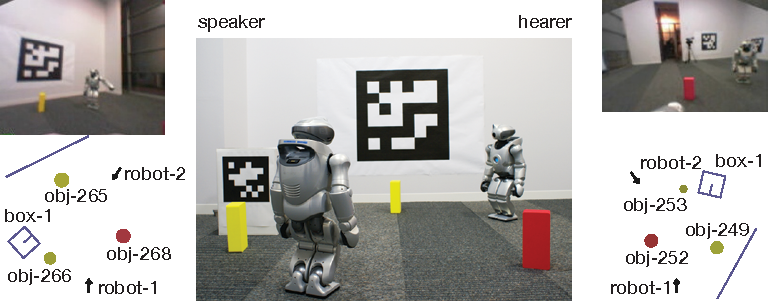
\includegraphics[width=.8\columnwidth]{figs/space-scene-2-small}
\end{centering}
\caption[Spatial setup example]
{Spatial setup}
\label{f:space-scene-2}
\end{figure}

\begin{figure}
\begin{centering}
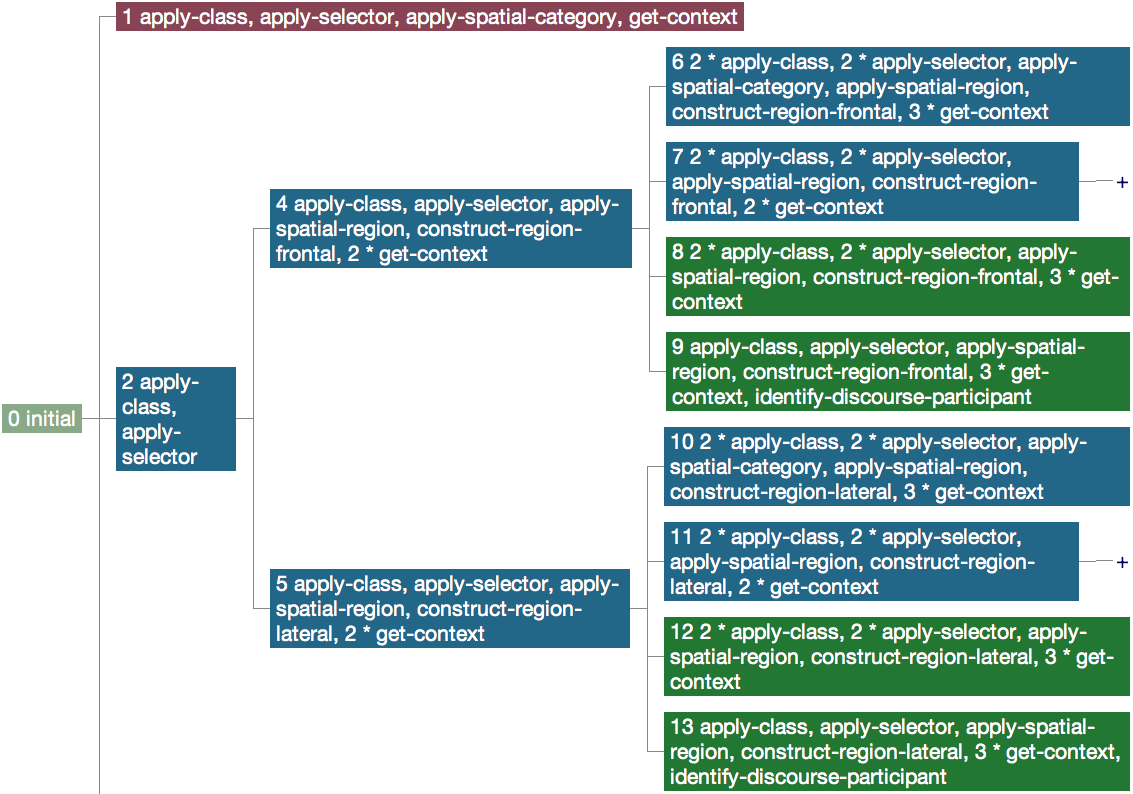
\includegraphics[width=1\columnwidth]{figs/conceptualization.png}
\end{centering}
\caption[Example search tree for conceptualization of a spatial scene.]
{Part of the conceptualization search tree for the spatial scene depicted
in \figref{f:space-scene-2}.
Some conceptualizations are rejected (red node), because they do not work
from the perspective of the hearer. This semantic structure in the red node 
in this figure corresponds to a determined spatial adjective noun phrase 
which is rejected because of the different
perspectives of the two robots on the scene. Green nodes 
show successful conceptualizations. In total around 30 conceptualizations 
for the topic are found which differ in degree of
applicability; some of them are more applicable than others.}
\label{f:conceptualization-search}
\end{figure}

\begin{figure}
\begin{centering}
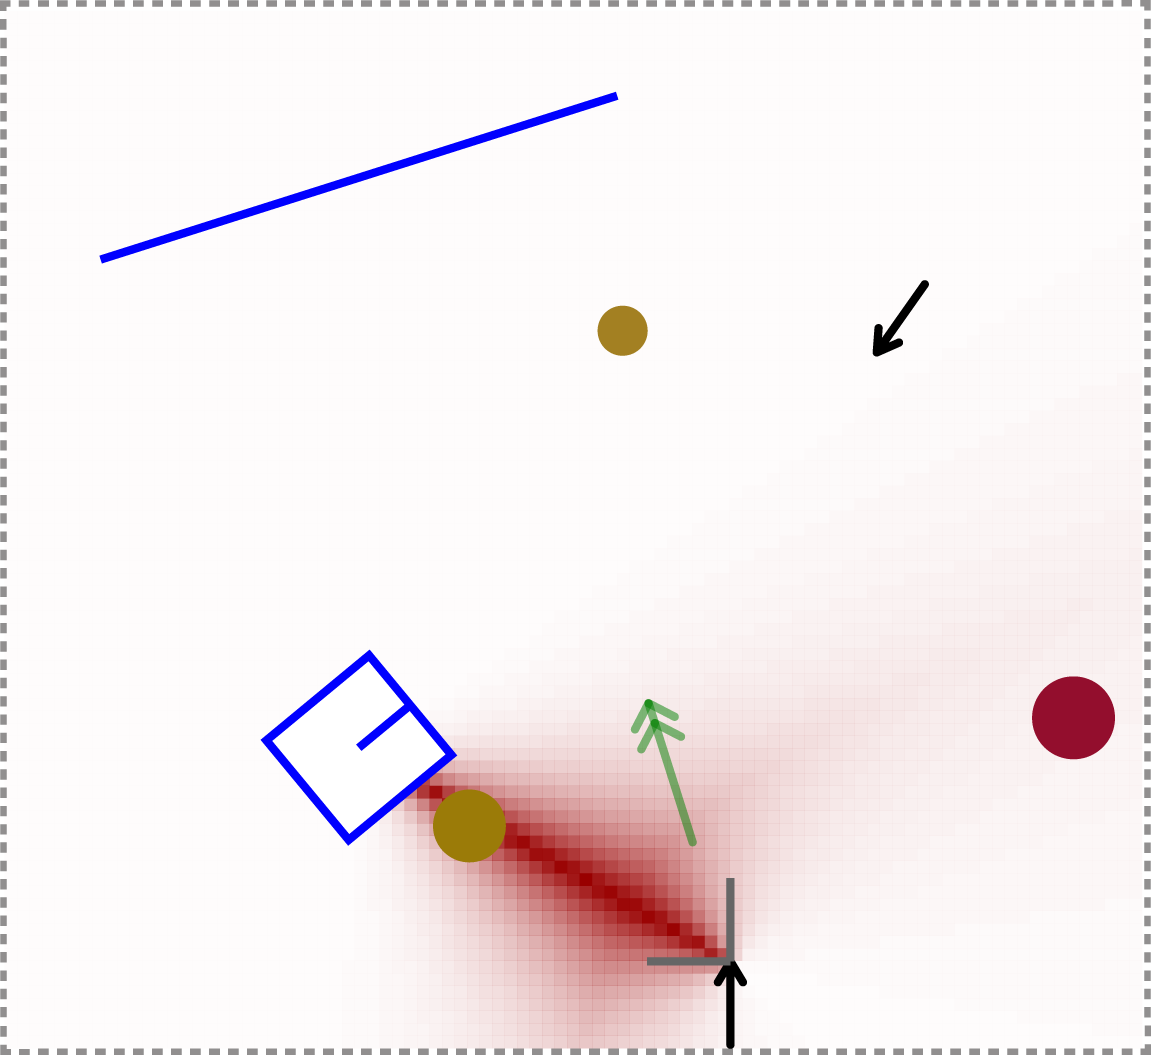
\includegraphics[width=0.25\columnwidth]{figs/conceptualization-in-front-of-the-box-from-my-perspective-region.png}
% \hspace{1pt}
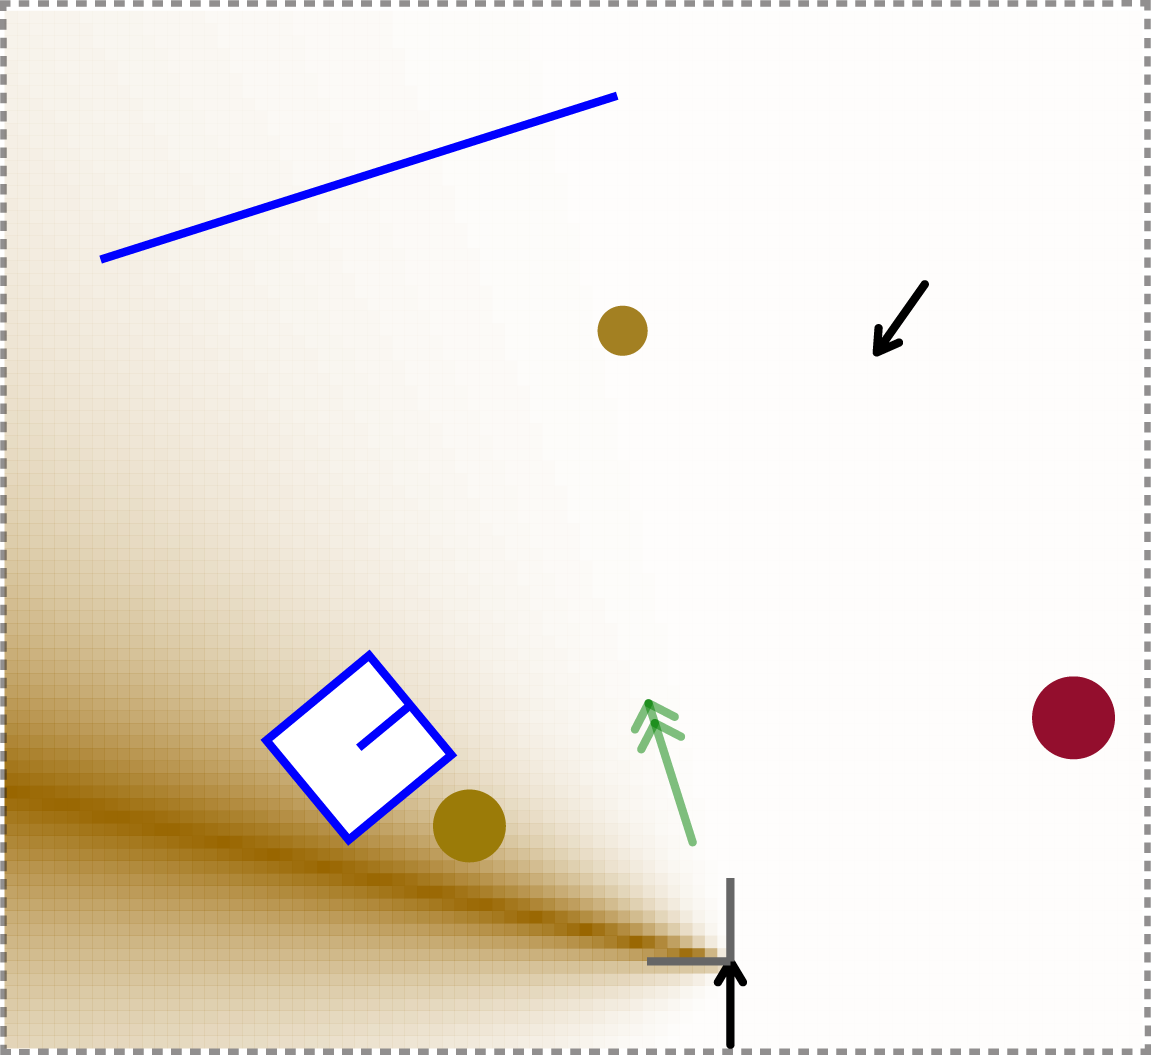
\includegraphics[width=0.25\columnwidth]{figs/conceptualization-right-of-me-from-your-perspective-region.png}
% \hspace{1pt}
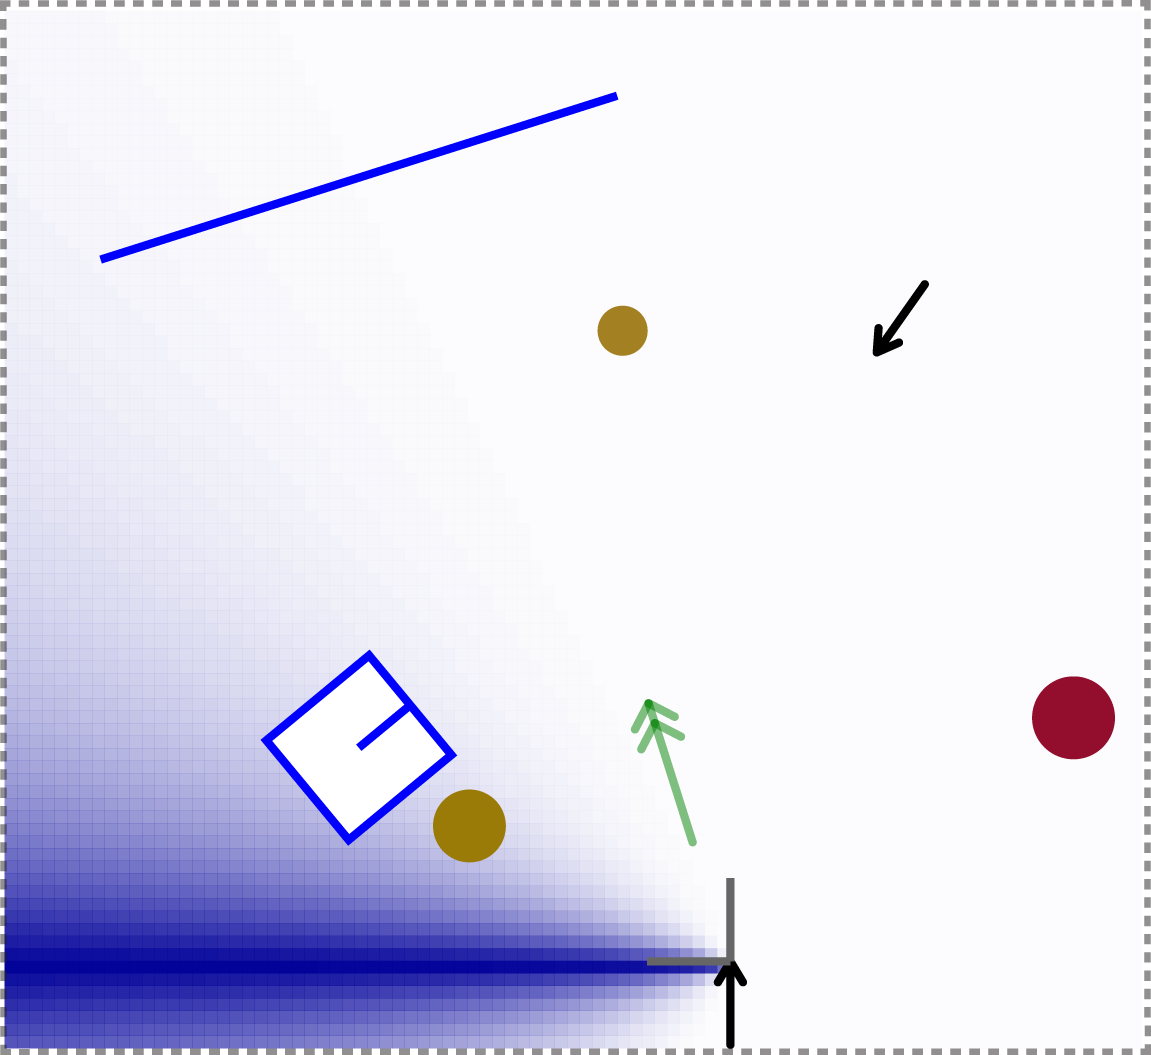
\includegraphics[width=0.25\columnwidth]{figs/conceptualization-left-of-me-region.png} \\
\vspace{1.5pt}
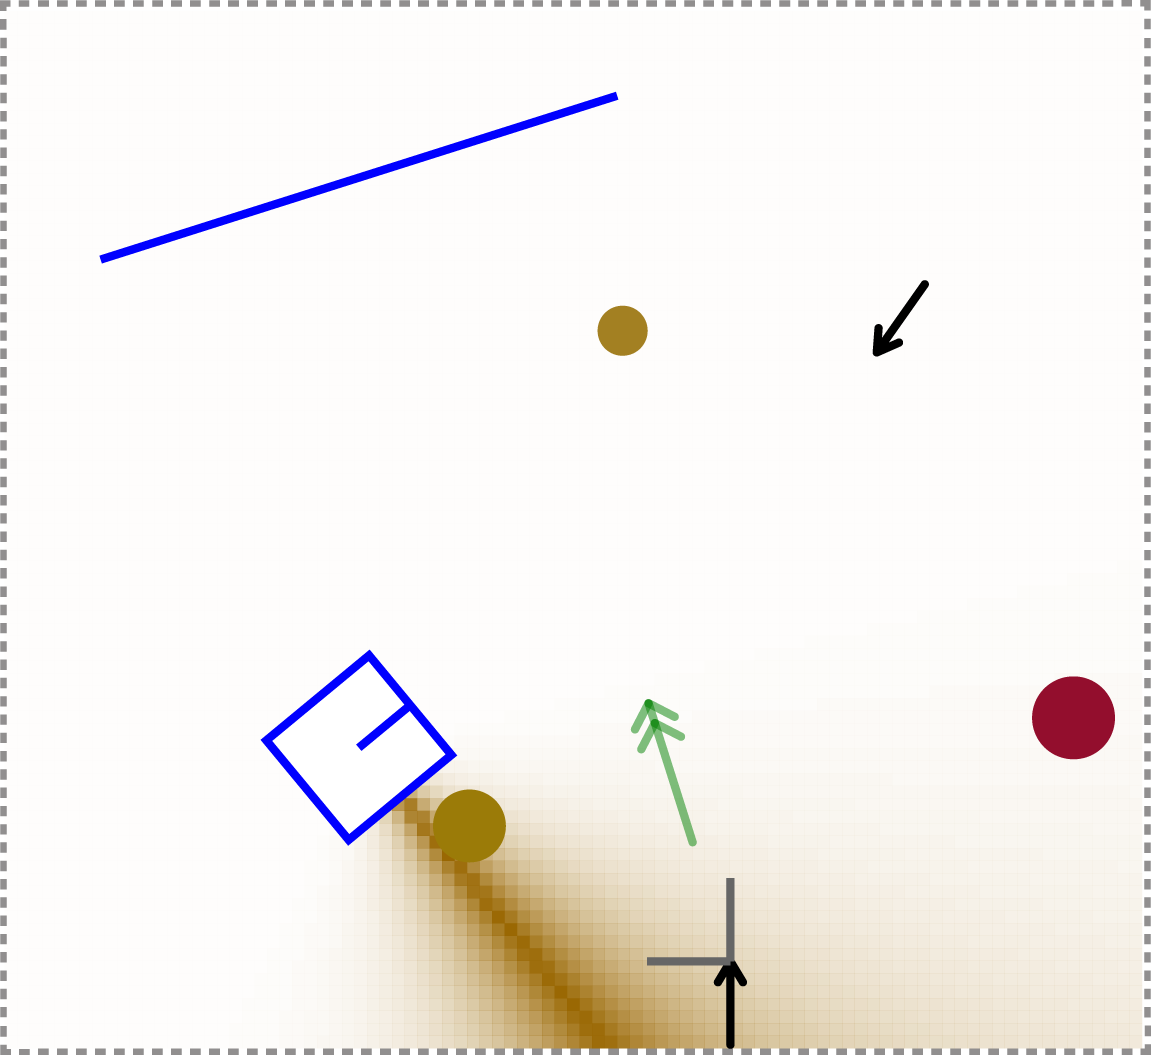
\includegraphics[width=0.25\columnwidth]{figs/conceptualization-right-of-the-box-region.png}
% \hspace{1pt}
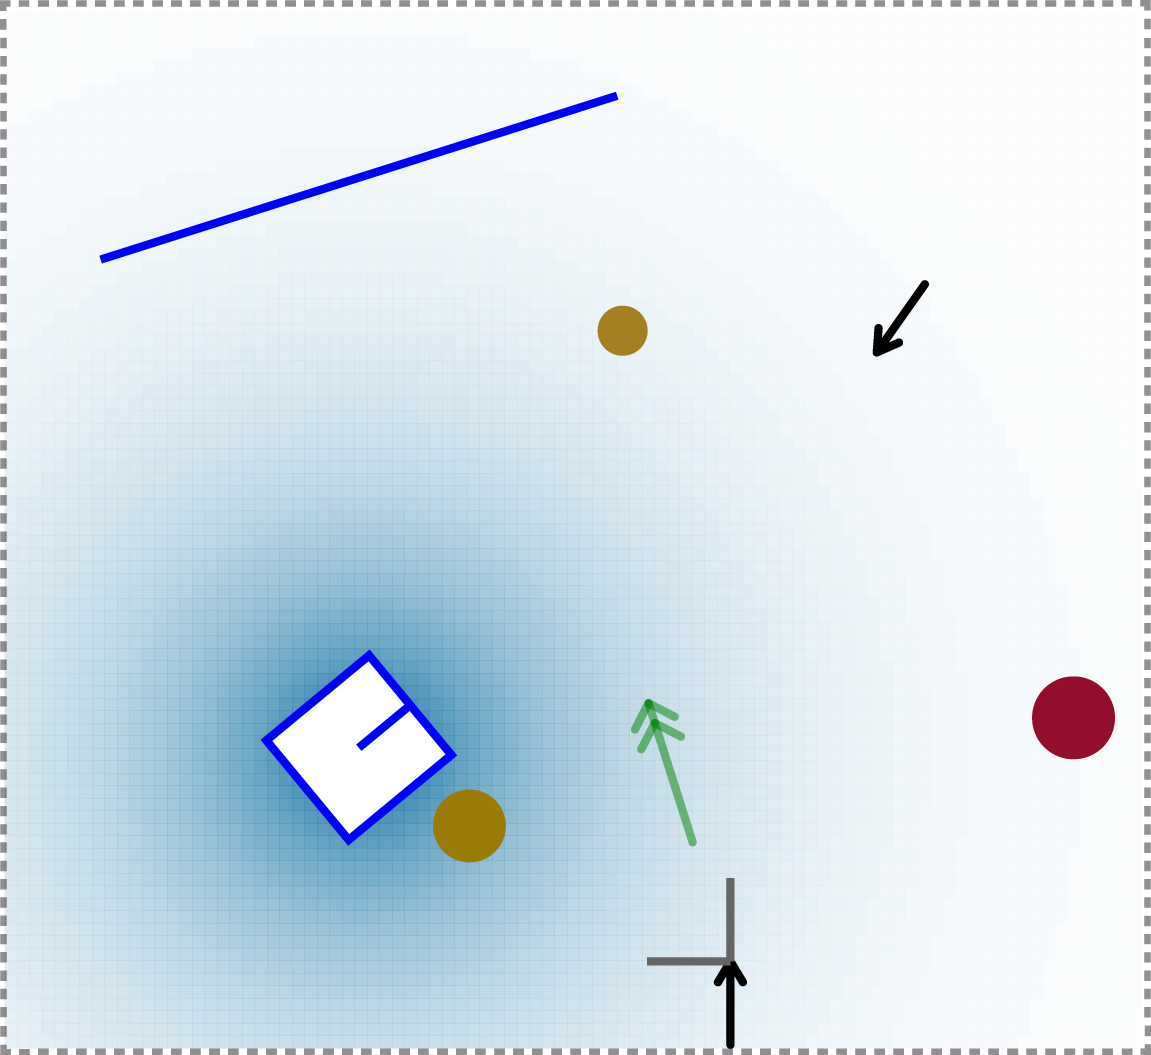
\includegraphics[width=0.25\columnwidth]{figs/conceptualization-near-the-box-region.png}
% \hspace{1pt}
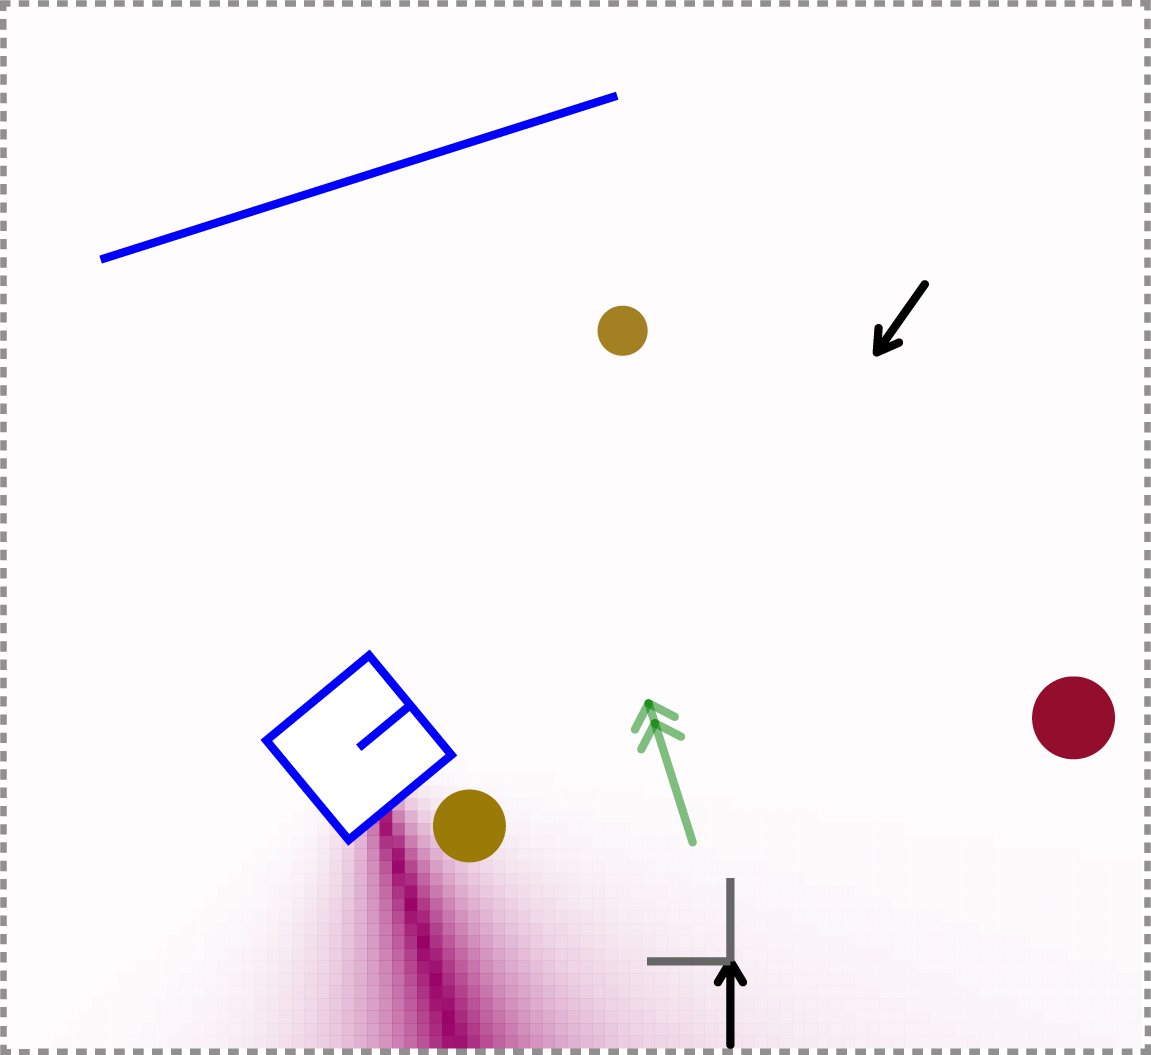
\includegraphics[width=0.25\columnwidth]{figs/conceptualization-south-of-the-box-from-my-perspective-region.png}

\caption[Conceptualization examples]
{The search process in \figref{f:conceptualization-search} finds more than
30 different conceptualizations for object {\footnotesize\tt obj-266} 
in the spatial scene depicted in \figref{f:space-scene-2}.
Some of them are depicted here in terms of regions that are 
described by the them. From left top to bottom right the figure
shows the regions used to discriminate the target object. In the
following, roughly corresponding utterances and discrimination scores
for the particular semantic structure are shown.\\
\begin{tabularx}{\linewidth}{r@{~}c@{~}>{\raggedright\arraybackslash}X}
0.55 & -- & \textit{der Block vor der Box von mir aus} \newline(`the block in front of the box')\\
0.50 & -- & \textit{der Block rechts von mir von dir aus} \newline(`the block right of me from your perspective')\\
0.38 & -- & \textit{der Block links von mir} (`the block left of me')\\
0.36 & -- & \textit{der Block rechts der Box} (`the block right of the box')\\
0.30 & -- & \textit{der Block nahe der Box} (`the block near the box')\\
0.23 & -- & \textit{der Block s\"udlich der Box} (`the block south of the box')
\end{tabularx}}
\label{f:conceptualization-results}
\end{centering}
\end{figure}

\section{Implementing spatial conceptualization}\label{sec:8.2}
Implementing the conceptualization of spatial scenes is based on 
two computational steps. Semantic structure is, first, automatically
combined and, second, it is ranked based on the particular
communicative goal. We use a search algorithm 
(see \chapref{s:irl}) as a means to 
automatically combine simple semantic building blocks 
into more complex ones. Semantic structure assembled in the search process is 
immediately tried on the current context, given the specific 
target object and rated based on how well it fulfills the communicative goal. 

\subsection{Ranking of semantic structure}
The scoring of semantic structure is guided by the communicative goal 
of the agent. For discrimination tasks, for example, the score of a particular 
semantic structure is mainly determined by how 
big the overall similarity of the target object is in contrast to 
the score of all other objects in the context. 
The \textsc{discrimination score} \is{discrimination score}
$\operatorname{disc}$ for the object $o$ with respect to other
objects $O$ is computed by subtracting the maximum
of all scores of the objects $o'$ in $O$ from the score $s_o$ of $o$.
\begin{eqnarray}
\operatorname{disc}_{o,O}=s_o - \max_{o' \in O}s_{o'}
\end{eqnarray}
The discrimination score is computed by evaluating the 
particular semantic structure whose discrimination score 
is to be determined and more specifically by evaluating the semantic operation 
{\footnotesize\tt apply-selector}. This operation singles out objects 
from sets of objects by choosing the object with the highest
similarity score and binding it with its discrimination score 
$\operatorname{disc_{o_{target},O}}$. 
For scoring semantic structure only the discrimination
score of the target object of the semantic structure is
of importance (see \figref{f:disc-score} for an example 
of accumulating similarities over a semantic structure).

\begin{figure}
\begin{center}
\includegraphics[width=0.8\columnwidth]{figs/semantic-structure-in-front-of-the-box-relative}
\includegraphics[width=0.8\columnwidth]{figs/semantic-structure-in-front-of-the-box-relative-evaluation}
\end{center}
\caption[Evaluation of semantic structure and discrimination scores]{%
Evaluation of semantic structure and discrimination scores. The top figure 
shows a semantic structure which is evaluated.
The bottom shows the bindings of variables resulting from evaluation. 
Objects have scores, and their scores are tracked and multiplied, which leads from the
context where every object has a score of $1.0$ to categorized sets such as the one
bound to {\footnotesize\tt ?landmarks} where the object class {\footnotesize\tt box} has been applied which 
results in all objects having a score of $0.0$ except for the box. Similarly, the region is applied
({\footnotesize\tt ?source-2}), followed by the application of the object class {\footnotesize\tt block}
({\footnotesize\tt ?source}). Finally, the topic ({\footnotesize\tt ?target}) is identified.}
\label{f:disc-score}
\end{figure}

Besides the discrimination score, other factors can be incorporated
into ranking semantic structure. For instance, one can include
the scores of categories and semantic entities, whether or not 
the semantic structure also would work if applied from the perspective
of the hearer, etc. The following is a non-exhaustive
list of the factors that can be included into ranking semantic
structure.

\begin{figure}
\begin{center}
\includegraphics[width=.8\columnwidth]{figs/semantic-structure-in-front-of-the-box-relative-evaluation-prediction-hearer}
\end{center}
\caption[Predictive evaluation from the perspective of the hearer]
{Predictive evaluation of the semantic structure shown in \figref{f:disc-score}. The speaker can test semantic structure how he thinks it 
would get evaluated by the hearer. In the case of the semantic structure shown
in \figref{f:disc-score} (top) the result of evaluation is object {\footnotesize\tt obj-265},
which is different from the target of the semantic structure when evaluated
from the perspective of the speaker (then it was object {\footnotesize\tt obj-266}).
In some sense this structure is ambiguous as to which object it refers to,
since the semantic structure is not explicitly perspective-marked.
On the other hand, the discrimination score of object {\footnotesize\tt obj-266} 
from the perspective of the
speaker is much higher ($0.55$) than the score for object {\footnotesize\tt obj-265} 
from the perspective of the hearer. In other words, if this would indeed be
the perspective of the hearer and not just a prediction, the agent could
choose to interpret {\footnotesize\tt obj-265} to be the target object.}
\label{f:predictiv-evaluation}
\end{figure}

\begin{description}
\item[Score of categories and semantic entities]
Categories and semantic entities such as frames of reference can be 
scored to reflect how 
conventional a particular item is. This allows to model preferences for
certain categories as, for instance, English native speakers show
preference for lateral over frontal categories, but also allows to 
capture \citep{tversky1999speakers}\index{Tversky, B.}\index{Lee, P.}\index{Mainwaring, S.} preferences for certain 
frames of reference. English speakers, for instance, 
have been observed to prefer the relative frame of reference
over the intrinsic one \citep{levinson2003space}\index{Levinson, S. C.},
and German speaker seem to prefer the intrinsic over the relative frame of reference 
\citep{ehrich1985linguistik}\index{Ehrich, V.}. Although evidence for these kinds of phenomena
seems at least contradictory (see \citealt{miller1976language}\index{Johnson-Laird, P. N.}\index{Miller, G. A.} for 
reverse findings for English speakers) nevertheless the assumption
that one frame of reference is conventionally selected more often 
is reasonable and can be incorporated into the 
scoring of semantic structure.
\item[Score of chunks]
Chunks -- the building blocks of semantic structure -- are themselves scored entities.
The score of chunks reflects how conventional or preferred a 
particular way of conceptualizing reality is. Languages, for instance, and their
syntactic regularities clearly reflect certain preferred conceptual choices. For instance,
in Russian, verbs always feature lexical Aktionsarten which conceptualize every event
in a way that highlights a particular aspect of that event, e.g. the beginning or the end or
that it repeats, etc. The syntactic need to express
these distinctions points to conceptualization strategies that are required to
build correct Russian sentences. Such strategies can easily be expressed with chunks
and their preference by scoring them accordingly \citep{gerasymova2010acquisition}\index{Gerasymova, K.}\index{Spranger, M.}.\is{measures!conceptualization strategy similarity}
\item[Perspective Choice]
In many situations speakers seem to prefer to conceptualize
reality from the perspective of the hearer. Social status and
cognitive abilities of the hearer \citep{mainwaring2003descriptions}\index{Ohgishi, M}\index{Tversky, B.}\index{Mainwaring, S.}\index{Schiano, D.}, 
as well as politeness \citep{schober1993spatial}\index{Schober, M. F.} 
and the question who is required to act \citep{tversky2009perspective}\index{Tversky, B.}\index{Hard, B. M.}
all have been observed to affect choice of perspective. Typically this
entails that the perspective of the addressee or hearer is preferred over
the perspective of the speaker. Choice of perspective is relevant for 
two cases of semantic structure. First, it is relevant for  
dealing with relative frames of reference and landmarks as in adverbial
and prepositional phrases in which the perspective on the scene 
overtly controls the way the scene is conceptualized. 
The other one is less obvious and relates to semantic structures that 
covertly depends on perspective such as 
group-based reference systems. In principle there are two ways 
to incorporate perspective into the ranking of semantic structure both of 
which rely on the fact that the speaker immediately tries semantic
structure from the perspective of the hearer. The first one is to outwardly
reject semantic structure that does not evaluate to the desired 
target object when evaluated from the perspective of the hearer or any
other desired perspective (see \figref{f:predictiv-evaluation} 
for an example of such a case). 
The other, more subtle one, is to compute the discrimination score
of the semantic structure from the perspective of the hearer. In other words,
while by default every agent uses his own perspective on the context
to score semantic structure, the robot now uses the perspective of the interlocutor.
To transform the context to the perspective of the hearer, each robot
continuously tracks the position of the interlocutor and subsequently
can use this information to evaluate semantic structure as he
predicts the interlocutor would execute the structure. Of course,
this is only a prediction in the sense that the speaker has
no certainty about the position of the interlocutor in the spatial
setup. Nevertheless, this is a hugely powerful device that
can eliminate many misunderstandings in communication 
before they occur. It is important to realize that in many situations
the choice of perspective has no or negligible effects
which is mainly true for contexts where 
the perspectives of the interlocutors overlap sufficiently.
Humans in such cases also do not mark perspective 
\citep{tenbrink2005dimensional}\index{Tenbrink, T.}.
Additionally, there are ways to even out the effect
of perspective by explicitly marking the perspective in the semantic
structure using the perspective transform operation
{\footnotesize\tt geometric-transform}. Such semantic structure
behaves like intrinsic or absolute spatial relations, since
the perspective is part of the structure. For spatial
adjectives this kind of marking of perspective
seems to be impossible in the sense that it cannot be conveyed
in language. In such cases a joint strategy by speaker
and hearer, for instance, the choice to always conceptualize from
the perspective of the hearer can be beneficial.

\item[Length of semantic structure]
Speakers thrive to be efficient in how
they communicate \citep{dale1995computational}\index{Dale, R.}\index{Reiter, E.}. The longer the 
semantic structure is for
discriminating a particular target object, the more needs to
be expressed in language. Length of semantic structure thus 
can be an important influence on the scoring of semantic structure.
Typically long semantic structures are punished.
\end{description}

These and other influences are easily incorporated 
into the scoring function of semantic structure which is the crucial
ingredient ultimately deciding which semantic structures from the vast space
of possible semantic structures are worth considering. 
The other important ingredient in implementing conceptualization 
is governing how semantic structure is assembled in the first place.
This process is one of automatic programming in which
chunks of semantic structure are combined based on 
input-output arguments. Figures~\ref{f:conceptualization-search} 
and~\ref{f:conceptualization-results} show the conceptualization 
search tree and some results of conceptualizing semantic 
structure for object {\footnotesize\tt obj-266} 
in the spatial scene depicted in \figref{f:space-scene-2}.

%\subsection{Additional Influences on Conceptualization not incorporated}
%discourse -> easily incorporated, however here no discourse
%representation

%%%%%%%%%%%%%%%%%%%%%%%%%%%%%%%%%%%%
\subsection{Ready-made semantic structure}
The size of chunks used in the conceptualization search process 
has a considerable influence on how elaborate
the search process in conceptualization has to be in order to find suitable
semantic structure for the particular communicative goal an agent might have.
In order to handle the large space of conceptualization, chunks can 
reflect various degrees of ready-made semantic structure with some 
being very large covering complete utterances such as determined spatial
adjective noun phrases, to smaller building blocks. How to choose 
the particular layout of chunks from the standpoint of designing
a running system is a decision that depends on how flexible the system
needs to be.


%%%%%%%%%%%%%%%%%%%%%%%%%%%%%%%%%%%%
\section{Categorization and discrimination}
\label{s:categorization+discrimination}
An important part of the complete machinery for discriminating an object
in the environment is the problem of how spatial categories and relations
themselves are applied. In computational modeling, discrimination is often conflated with categorization,
or to be more precise, with a certain approach to categorization which can 
be called \textsc{strict category membership}\is{categorization!strict} (see \citealt{belpaeme2007language}\index{Bleys, J.}\index{Belpaeme, T.} 
for an application of this approach to color). Categorization is understood here
as strict membership in which a point in the sensorimotor 
space is categorized as belonging
to the one category closest to him. For instance, an 
object is considered to be red, when red is the color category 
that is most similar to it. If this is the case the object is a member
of the red category. Consequently, every point in the sensorimotor space 
belongs to precisely one category of the set of categories and the
complete sensorimotor space can be decomposed 
into different sets of objects based on their category membership, 
a process known as Voronoi tesselation (\citealt{aurenhammer1991voronoi}\index{Aurenhammer, F.}, see \figref{f:voronoi}).
Applying such an approach to discrimination, one needs to additionally 
define some criteria as to when a category $c$ can be called discriminating
object $o$ from the context $O$. The strict category membership approach
posits two requirements to be met.
\begin{description}
\item[Strict membership] $o$ is said to be a strict member of the category $c$, iff
 $o$ is closer to $c$ than to any other category from the repertoire of categories $C$.
 In order for $c$ to be called to discriminate $o$, $o$ has to be a strict member of $c$.
\item[Discriminating category] In order for $c$ to be discriminatory,
$o$ has to be the only object from the context $O$ that is a strict member of the category
$c$.
\end{description}
Of course, the first criteria is a necessary condition for the second to apply,
but in terms of objections that I will discuss following this approach, 
it makes sense to consider both of them separately. 

There are two lines of arguments why such an approach to discrimination
is wrong. First, there is accumulating evidence from natural language that
is in conflict with both criteria. For instance, many scholars propose
alternative principles particularly in conflict with the discriminating 
category criteria. Rather then requiring $c$ to be the only category 
closest to $o$, they require that $o$ is the closest object to $c$ 
without further constraining the other objects in $O$ and their relationship
to $c$. So other objects in $O$ can be strict members of $c$ as long as they
are not closer to $c$ than $o$. In fact what seems to be driving
people in their choice of categories in discrimination task seems to be most
importantly the principle of \textsc{greatest distance} or greatest 
contrast \is{greatest distance principle}\is{greatest contrast|see{greatest distance principle}} 
which only requires the category to establish sufficient difference
between the distance of object $o$ and all other objects in the context.
Such principles have been used generally to explain peoples behavior in 
object discrimination tasks \citep{hermann1976objektbenennung}\index{Hermann, T.}\index{Grabowski, J.}
and also have been applied more specifically to spatial language 
(see the \textsc{shifting contrast principle} \is{shifting contrast principle|see{greatest distance principle}}introduced by 
\citealt{herskovits1986language}\index{Herskovits, A.} and similar ideas in \citealt{freksa1999links}\index{Freksa, C.}).
These insights primarily relate to criterion two. But one can also use them 
to attack the strict membership criterion. If humans really
are looking for categories that establish high contrast, the assumption
that $o$ has to be closest to the category $c$ in order for $c$ to be
even considered clearly has to be wrong. For instance, $c$ might not
be the category that is closest to $o$, however, if it establishes enough 
contrast between $o$ and all other objects in the context it does not 
have to be. This seems to be the case for spatial language. 
\cite{tenbrink2005identifying}\index{Tenbrink, T.}, for instance, found that unmodified 
projective terms are frequently used by participants in a discrimination task
for referring to objects that are far away from the prototypical axes. Now clearly
in such tasks the linguistic material available to natural language speakers 
allows them to be much more precise about the actual spatial position
in the sense claimed to be relevant by the strict membership criterion.
In other words, speakers could choose to describe a spatial relation 
for objects based on smallest distance to some prototypical point, but they
choose not to. So there seems to be some empirical evidence that
speakers behave differently than claimed by these two principles.

The second line of arguments against the strict category membership 
approach to discrimination comes from computational modeling. In particular, we
can compare the approach advocated in this book with the strict category membership \index{strict category membership|see{categorization!strict}}
to discrimination and show that it performs better
in real-world scenarios. To be able to compare the two approaches
we obviously need an implementation of both. I have already sketched
the approach in the previous chapters, and I will sketch the implementational
details of the strict category membership approach in the following paragraphs.

\begin{figure}
\begin{center}
\includegraphics[width=0.3\columnwidth]{figs/voronoi}
\end{center}
\caption[Voronoi tesselation]{Decomposition of a metric space into different parts.
Every point in the plane is categorized based on which
centroid (black dots) it is closest leading to subsets of
points where all points are closest to a particular centroid (Figure adapted from 
\citealt{aurenhammer1991voronoi}\index{Aurenhammer, F.}).}
\label{f:voronoi}
\end{figure}

\subsection{Strict category membership}
Implementing such a notion of categorization has a profound 
impact on the processing of semantic structure. Instead of computing 
similarities and adding them to objects as in the lenient approach, categorization 
is implemented as a set of filter-operations which take some input set and filter the 
objects in the input set given a particular category which results in an 
output set only containing objects that are closest to that category (see 
\figref{f:filtering-operations} for an example of semantic structure with 
filtering operations). When evaluating a semantic structure
consisting of such filter operations, the set of objects in the context progressively
shrinks by applying subsequent filtering operations until one object is left, 
the topic or target of the semantic structure. For example, 
in the semantic structure shown in \figref{f:filtering-operations}, first
{\footnotesize\tt get-context} will introduce the set of objects perceived by
the robot, followed by the filtering of blocks, which results in the
set of blocks of the context. Afterwards, 
{\footnotesize\tt filter-by-spatial-category-group-based} will compute the centroid
of the group-based landmark, followed by the application of the 
spatial category {\footnotesize\tt left} to that landmark, which results in the
filtered set of ``left blocks''. The selector {\footnotesize\tt unique} only
checks whether the set of ``left blocks'' only contains one
object and if that is the case outputs that object.

This way of modeling semantic structure bears some similarities with
logic based approaches to semantics where, for instance, noun phrases denote a 
property that can be represented as a function from entities to truth 
values (see for example \citealt{barwise1981generalized}\index{Cooper, R.}\index{Barwise, J.}) -- in other words, where noun phrases denote sets of objects for which
the property holds. For instance the interpretation of \textit{Ball} (`ball') denotes 
the set of all balls in the context which is the same as filtering the context
for the set of balls. Such approaches are the dominant way of semantic
analysis for instance in generative grammar and they are also applied 
by many scholars to the semantic analysis of spatial language (see 
\citealt{eschenbach1997axiomatic}\index{Eschenbach, C.}\index{Kulik, L.} for an example). Consequently
one is tempted to take such an approach to modeling the semantics
of spatial language. However, there are some considerable problems
associated with the category membership approach particularly when 
facing the problem of \textsc{perceptual deviation}.\is{perceptual deviation}

\begin{figure}
\begin{center}
\includegraphics[width=.8\columnwidth]{figs/semantic-structure-filtering-der-linke-block}
\end{center}
\caption[Category membership semantics]{On the left side, the semantic structure of the phrase 
\textit{der linke Block} (`the left block') with {\footnotesize\tt filter} operations is shown. The images to 
the right show the progressive filtering of the set of objects in the context when the 
semantic structure is evaluated. The context {\footnotesize\tt ?ctx} contains all objects
perceived by the robot, whereas the set {\footnotesize\tt ?blocks} contains all blocks
filtered from the context and, finally, the set {\footnotesize\tt ?left-blocks} 
only consists of the object {\footnotesize\tt obj-230}.}
\label{f:filtering-operations}
\end{figure}

\begin{figure}
\begin{center}
\includegraphics[width=.8\columnwidth]{figs/semantic-structure-apply-der-linke-block}
\end{center}
\caption[Lenient categorization semantics]{\is{categorization!lenient}%
On the left side, the semantic structure of the phrase
\textit{der linke Block} (`the left block') with {\footnotesize\tt apply} operations is shown. The images to
the right show the application of semantic operations which leads to the
bindings of the variables {\footnotesize\tt ?ctx}, {\footnotesize\tt ?blocks} and {\footnotesize\tt ?left-blocks}
with progressively changing similarity scores. For this example similarities are
multiplied. First the operation {\footnotesize\tt apply-class} is evaluated leading to
scores of for all entities of type block and
for all others. Next the spatial operation {\footnotesize\tt apply-spatial-category-group-based}, 
which computes spatial similarities based on a landmark is executed.
Consequently all objects in the {\footnotesize\tt ?left-block} entity set are scored with
indeed the left block object {\footnotesize\tt obj-230} having the highest
overall score.}
\label{f:apply-operations}
\end{figure}

While the target entity of the semantic structure in \figref{f:filtering-operations} 
is essentially the same as, for instance, for a comparable structure using the 
approach advocated in this book (see \figref{f:apply-operations}),
in many cases the category membership 
approach is bound to fail due to noise and uncertainty in the 
estimation of spatial distances and angles or other perceptual
data channels such as color. The problem is that no two robots perceive
the world in the same way. Colors, sizes, distances and 
angles are all estimated using
complicated visual processing which is subject to noise and uncertainty, which
makes for instance the distance of one object to another appear smaller
for one of the robots in the scene. For instance, in \figref{f:space-scene-2}
object {\footnotesize\tt obj-266} (which is object {\footnotesize\tt obj-253} in the world model 
of the hearer) is smaller and more to the right of the box, than in the world model
constructed by the hearer. In the case of strict category membership these
sorts of perceptual deviations can lead to problems in interpretation.
Even if grammar would allow for perfect transmission of a semantic structure,
in other words, even if there would be no ambiguity or problems
in linking when parsing a phrase like \textit{der Block rechts der Kiste}, the
evaluation of the underlying semantic structure can lead to misunderstanding, 
i.e. both robots think that the utterance is about different objects. 
The reason for this type of misunderstanding is the strict filtering of sets
underlying interpretation of phrases in the category membership
approach. While for the speaker the object in question, for instance 
{\footnotesize\tt obj-266} is still to the right of the box, this might not necessarily 
be true in the world model of the hearer, which can lead to no or false 
interpretations of the semantic structure. Consider 
\figref{f:perceptual-deviation}, where object {\footnotesize\tt obj-212}
for the speaker is to the intrinsic left of the box, whereas it is to the
intrinsic right for the hearer. Small estimation errors in judging
distance and angle can thus lead to very different categorizations of 
the same object.

\begin{figure}
\begin{center}
\includegraphics[width=0.5\columnwidth]{figs/perceptual-deviation}
\end{center}
\caption[Perceptual deviation]{Example for perceptual deviation and
impact on filtering operations}
\label{f:perceptual-deviation}
\end{figure}

\subsection{Lenient approach}
In contrast to the strict category membership, the approach 
advocated in this book does not rely on category membership, 
but only considers similarities to categories without enforcing the strict
membership criteria. In other words an object does not have to be closest
to the category {\footnotesize\tt left} in order to be categorized as left. Only one 
thing is important: the object needs to have a bigger similarity with 
{\footnotesize\tt left} than any other object in the context (see Figure 
\ref{f:apply-operations} which shows the accumulation of scores).
From this fact alone one can predict that the lenient approach
is better suited for dealing with perceptual deviation, as it is less 
restrictive in interpretation. But another prediction can be made as
well. The approach is also less restrictive in conceptualization,
in the sense that the strict category membership constraint is
also not applied in finding a category to discriminate an object.
Consequently, the lenient approach should also be able 
to find semantic structure in cases where the strict membership
approach fails as its membership constraint cannot be met.

\begin{figure}
\includegraphics[width=0.6\columnwidth]{figs/lenient-vs-strict-interpretation}\\
\includegraphics[width=0.6\columnwidth]{figs/lenient-vs-strict-interpretation-strict}\\
\includegraphics[width=0.6\columnwidth]{figs/lenient-vs-strict-interpretation-lenient}
\caption[Lenient vs strict categorization]{\is{categorization!strict}%
Lenient versus strict categorization\is{categorization!strict}.
The first figure shows 
the similarity functions for {\footnotesize\tt left} and {\footnotesize\tt right} 
categories over the angle. The second figure shows the decomposition
of the angular space using the strict approach. The third figure shows
how the lenient approach uses the similarity function of the spatial category
to retrieve the correct object.}
\label{f:lenient-vs-strict}
\end{figure}

Figure \ref {f:lenient-vs-strict} contrasts the example in Figure \ref{f:perceptual-deviation} 
from the viewpoint of strict and lenient discrimination. The top figure shows 
the similarity functions for {\footnotesize\tt left} and {\footnotesize\tt right} categories over the angle, 
from which the decomposition of the angular space show in the middle Figure follows.
The particular similarity function of the two categories interact in the decomposition
of the space. Object {\footnotesize\tt obj-212} is categorized by the speaker as being to the
left, whereas the same object for the hearer which he knows as object {\footnotesize\tt obj-240} is 
to the right. When the speaker thus conceptualizes the object as left, the hearer has no 
chance of retrieving the object in the strict interpretation case. On the other hand, when
applying a lenient discrimination scheme (bottom figure) there is no interaction 
between the categories {\footnotesize\tt left} and {\footnotesize\tt right}.
The decision whether or not the hearer is able to discriminate the correct object
depends on whether object {\footnotesize\tt obj-240} is indeed the most similar object
to the category {\footnotesize\tt left} (which it is in this case). To ensure that agents
can always find the correct object, category similarity functions always
span across the complete space. For instance, for the angular category
{\footnotesize\tt left} every angle has a similarity bigger than zero. For some angles
similarity is small, but importantly it is never below zero.

\subsection{Experimental setup}
We can study the difference of the two approaches systematically by letting agents
interact in controlled spatial scenes and see
which of the two approaches performs better in a discrimination task. 
In order to to study only the effect of the particular implementation of semantic 
operations, I eliminate the influence of language using 
direct meaning transfer, in which the hearer is passed the
semantic structure conceptualized by the speaker without going
through production and parsing of syntactic structure. 
This is equivalent to having 
a language where sufficient information is provided in each utterance
to decode the semantic structure intended by the speaker 
without uncertainty, ambiguity or loss of information.
The particular interaction script used in the experimental
setup is the following. Always two agents from a population interact. 
One is the speaker, the other the hearer. The speaker perceives the world,
picks a topic and tries to conceptualize a semantic structure
for reaching his communicative goal. If he is successful in finding
semantic structure for discriminating the topic, he passes the semantic
structure to the hearer. The hearer interprets the semantic structure
by simply evaluating it. Afterwards he points to the object he
thinks the semantic structure was about. 

Thus, there are four different outcomes of the game.
\begin{description}
\item[Conceptualization failed] After the speaker choose a topic, he has
to conceptualize a semantic structure that discriminates the topic.
This process fails, if the speaker cannot find any semantic structure
that allows him to discriminate the object from all other objects in the
context.
\item[Interpretation failed] After the speaker successfully conceptualized
a discriminating semantic structure, the hearer interprets this structure
by simply evaluating the semantic program. If this evaluation
yields no result, the hearer is said to have failed.
\item[Pointing failed] When the hearer successfully interpreted the
semantic structure passed to him by the speaker, he points
to the topic he interpreted. The speaker then interprets whether
the object pointed to is indeed the topic. If this is not the
case then pointing failed.
\item[Success] The hearer pointed to the correct object and
the game is a success. 
\end{description}

We can compare the two approaches to categorization 
using two different sets of agents --
one in which agents are equipped with a lenient implementation 
of semantic operations as advocated in this book, and a second where
agents are equipped with category membership based
semantic operations. Both agents were equipped with
complex semantic structure, which allowed them to use
group-based reference, landmarks, relative and intrinsic frames
of reference together with proximal and projective spatial categories
implemented as in the German space semantics discussed in 
\chapref{s:german-space-semantics}. I test both populations and 
their respective success and failure on different sets of spatial scenes.

\begin{figure}
\begin{center}
\includegraphics[width=.8\columnwidth]{figs/apply-filter-comparison-scenes}
\end{center}
\caption[Spatial scenes used to compare lenient vs. strict categorization]
{\is{categorization!strict}\is{categorization!lenient}%
This figure exemplarily shows spatial scenes used for comparing lenient and strict
categorization implementations. The left image shows an example scene from the data 
set labeled {\footnotesize\tt space-game-10} which consists of scenes with one landmark and two robots 
that can be used as reference systems. Spatial scenes in data set {\footnotesize\tt space-game-17} (middle image) consist of scenes without boxes.
Only the two robots and group-based reference are available for conceptualizing the spatial
scene. The right image shows an example from data set {\footnotesize\tt space-game-18} which features a box 
just as {\footnotesize\tt space-game-10}, but in much more complex spatial layouts.}
\label{f:lenient-vs-strict-scenes}
\end{figure}

\subsection{Results}
The results in \figref{f:apply-filter-comparison} show
a clear advantage for the lenient approach proposed in this 
book. The success in interaction for this approach to 
spatial categorization is consistently above 85\% across various 
spatial scenes, whereas the success of strict categorization\is{categorization!strict} drops to 22\%
in the worst case ({\footnotesize\tt space-game-18}) but consistently performs below 60\%
success showing the power of the lenient approach to deal even with 
very complex spatial scenes (see \figref{f:lenient-vs-strict-scenes} for
some example scenes from the different spatial scenes). Notably,
the lenient approach in almost all scenes is able to successfully conceptualize
the spatial scene for the topic in question. Only few cases in data set {\footnotesize\tt space-game-18}
are marked for failure in conceptualization. On the other hand, the strict
approach shows enormous problems even conceptualizing for particular
objects in particular scenes. Almost all cases of failure are either due to 
failures of conceptualization or failures of interpretation, where conceptualization
as can be seen takes the major blame for failure.

\begin{figure}
\begin{center}
\includegraphics[width=.8\columnwidth]{figs/apply-filter-comparison}
\end{center}
\caption[Comparison of filter type semantics and apply semantics]
{Results of comparing strict versus lenient categorization\is{categorization!lenient}
on different sets of spatial scenes}
\label{f:apply-filter-comparison}
\end{figure}
% [todo: add condition names and svg's]

Failures to conceptualize in the case of strict category membership are caused by 
insufficient clustering of the input space. The problem is that categories are not
dense enough to allow the speaker to conceptualize for the particular topic.
Failures to interpret on the other hand are caused by perceptual deviation.
Strikingly, there are no interpretation failures in the case of the lenient approach
highlighting its power to deal with perceptual deviation. Maybe for the strict
approach the problem could be eased. For instance one could increase
the number of possible decompositions of the sensorimotor space
by adding more categories which allows the speaker to more easily conceptualize.
\figref{f:filter-increased-categories} shows the effect of 
adding more categories to the inventory of strict categorization\is{categorization!strict} agents.
It compares four conditions (over the different spatial scenes):
``german'', ``double'', ``triple'' and ``quadruple''.
``German'' refers to the set of categories introduced earlier, e.g. front, back, left, 
right and so forth. ``Double'' refers to a set of categories where the number of 
categories is doubled. So for instance, instead of two lateral categories left and right 
there are now four. The same holds for frontal and proximal categories. In the ``triple'' 
condition agents are equipped with three times as many categories and in the
``quadruple'' condition the number of categories is four times compared to the 
german condition. 

In some cases most notably for data set {\footnotesize\tt space-game-18} 
more categories indeed helps triple the success in interaction. This is not all that
surprising in the sense that there was a lot of room for improvement in the 
first place. For the other two sets of scenes success in interaction stays 
pretty much the same. And it seems that also for {\footnotesize\tt space-game-18} a certain
limit of improvement is reached, as success actually drops again for quadrupled
number of categories\is{measures!number of categories}. The most interesting point is, however, that overall 
success in interaction stays roughly the same for most spatial scenes 
and failures of the speaker to conceptualize
are replaced by the inability of hearers to interpret. This is most strikingly the case
in condition {\footnotesize\tt space-game-17} where this type of error accounts for 20\% of all
interactions and half of the unsuccessful ones. In other words, the more categories 
there are available, the more impact perceptual deviation has on the strict set approach.
The reason for this can be found in the interaction of categories that determines 
the decomposition of the space. The more categories there are, the smaller the 
area of applicability of categories
becomes, and consequently the more likely it becomes that an object that is
categorized as belonging to a certain category by the speaker will be 
categorized differently by the hearer. One might
wonder what the effect of more categories is on the lenient categorization\is{categorization!lenient}
approach. \figref{f:apply-increased-categories} shows that while there
is some impact of more categories in the difficult scenes of data set
{\footnotesize\tt space-game-18}, overall there is no significant increase in success in
interaction.

\begin{figure}
	\begin{center}
		\includegraphics[width=.8\columnwidth]{figs/filter-more-categories.pdf}
	\end{center}
	\caption[Effect of additional categories on strict categorization]
	{Results of comparing different sets of spatial categories and their 
		effect on the strict categorization\is{categorization!strict} approach}
	\label{f:filter-increased-categories}
\end{figure}
\begin{figure}
	\begin{center}
		\includegraphics[width=.8\columnwidth]{figs/apply-more-categories.pdf}
	\end{center}
	\caption[Effect of additional categories on lenient categorization]
	{Results of comparing different sets of spatial categories and their 
		effect on the lenient categorization approach.\is{categorization!lenient}}
	\label{f:apply-increased-categories}
\end{figure}

%%%%%%%%%%%%%%%%%%%%%%%%%%%%%%%%%%%%
\section{Summary}
We can conclude that the communicative intentions of an agent influence
how spatial scenes are conceptualized, i.e. which spatial relation is chosen, 
which frame of reference, or which landmark. The most important
factor is whether an agent wants to discriminate or describe an object.
But, preferences for particular spatial relations, perspective or frames of 
reference are also important. This chapter showed that these factors
are easily operationalized using IRL. Experimental results demonstrate that the system
is powerful enough to enable robotic agents to reliably conceptualize 
spatial reality. The results of this chapter are further discussed in \cite{pauw2010embodied,pauw2012embodied,spranger2012deviation}.\index{Spranger, M.}\index{Pauw, S.}



% \bibliographystyle{diss}
% \bibliography{papers,space}
% \end{document}

 %\documentclass[]{diss}
%\begin{document}


\chapter{A Whole Systems Approach to Processing}
\label{s:german-locative-phrases-syntax-semantics-integration}
So far I have discussed processing of German locative phrases
isolated for semantics and syntax. However, IRL and FCG are systems that 
have to work together to allow agents to talk. This chapter reflects on the 
integration of these two systems in a unified architecture. 
Consequently this chapter is technical in nature. It starts out by giving
an overview of how processing is integrated (Section \ref{s:irl-fcg-integration}).
Section \ref{s:semantic-ambiguity} discusses the phenomenon of 
\emph{semantic ambiguity}\index{semantic ambiguity} which requires a deep level of integration.
The chapter concludes with results on the performance of the 
complete system (Section \ref{s:syntax+semantics-integration}).


\section{Integrating IRL and FCG}
\label{s:irl-fcg-integration}
IRL and FCG are integrated via a mechanism which is called 
the \emph{task engine}\footnote{All computational systems described in this 
book are integrated into a framework for running and evaluating 
experiments described in \cite{steels2010babel}\index{Steels, L.}\index{Loetzsch, M.}.}.
The task engine bundles the processing done by an agent and allows to track
different hypotheses. For instance, in production a speaker might conceptualize
different semantic structures and only later decides which of those he wants
to use based on how well it can be verbalized. For this IRL and FCG 
is packaged into processes.
\index{task processor}
\begin{figure}
\begin{center}
\includegraphics[width=0.8\columnwidth]{figs/production}
\caption[Processes running when a speaker produces an utterance]{
Processes running when a speaker produces an utterance. Ellipsis are
data structures. Squashed rectangles are processes.}
\label{f:production}
\end{center}
\end{figure}

Figure \ref{f:production} and \ref{f:interpretation} show the typical processing 
for the speaker and the hearer.
Each of them runs different processes which bundle FCG 
and IRL for production and interpretation. The most 
important processes are 
\begin{description}
\item[conceptualize] This process takes as input the world model (context) computed 
by the vision system and a topic object. Using these input 
arguments an ontology and a set of known chunks, the process uses the 
IRL search to produce one or several possible IRL-networks.
\item[produce] This process applies constructions in the direction of production.
In other words, matching happens on the semantic side. Production takes as input
an IRL-network and a set of constructions and produces one or more possible utterances
using FCG's search process.
\item[parse] Parsing is the process which takes a set of constructions and an utterance
and computes one or more possible interpretations, i.e. IRL-networks.
\item[find-topic] This process uses IRL to compute a topic based on 
an IRL-network and the context (computed by the vision system).
\end{description}
All of these processes can produce one or many outcomes. The task engine
branches on multiple results. For instance, when \emph{conceptualize} has found
different IRL-networks, the engine tracks their individual success in separate 
\emph{produce} processes. The overall best result is determined by 
combining the discrimination score of the meaning and confidence of construction 
application. Moreover, as we can see in Figure \ref{f:production} speakers also run processes vital 
for the hearer. Before passing an utterance to the hearer, the speaker parses and
interprets the phrase he is about to use. The mechanism is called 
\emph{re-entrance}\index{re-entrance} \citep{steels03reentrance}\index{Steels, L.}. Applied to this process model,
this means that agents can choose the best result based on the 
prediction how that phrase might be interpreted by the hearer.

\begin{figure}
\begin{center}
\includegraphics[width=0.7\columnwidth]{figs/interpretation}
\caption[Processes running when a hearer interprets an utterance]{
Processes running when a hearer interprets an utterance. Ellipsis are
data structures. Squashed rectangles are processes.}
\label{f:interpretation}
\end{center}
\end{figure}

\section{Handling Semantic Ambiguity}\index{semantic ambiguity}
\label{s:semantic-ambiguity}
An example where the integration of the systems for syntactic processing
and conceptualization can play out its power is \emph{semantic ambiguity}.
A phrase is semantically ambiguous if multiple semantic structures, i.e. IRL-networks,
can be interpreted. 

% german locative phrases - syntactic and semantic ambiguity
Many German locative phrases are semantically ambiguous.
Let us consider the following two examples from German.
\begin{example}
\label{e:der-block-vor-der-linken-kiste}
\gll der Block vor der linken Kiste 
the.NOM block.NOM front.PREP the.DAT left.ADJ.DAT box.DAT.FEM 
\glt `The block in front of the left box'
\glend
\item
\label{e:der-block-vor-der-linken-kiste-von-dir-aus}
\gll der Block vor der linken Kiste von dir aus 
the.NOM block.NOM front.PREP the.DAT left.ADJ.DAT box.DAT from.PREP your.DAT perspective 
\glt `The block in front of the left box from your perspective'
\glend
\end{example}
Example \ref{e:der-block-vor-der-linken-kiste} is semantically ambiguous with 
respect to how the landmark object, in this case \emph{the left box}, is 
conceptualized. The phrase can have an intrinsic or relative reading.
The second example does not have this problem. 
The perspective marker clearly signals a relative reading of the phrase.
Interestingly, this fact can only be established after parsing the complete phrase. 
To illustrate this dependency consider Example  \ref{e:der-block-vor-der-linken-kiste-von-dir-aus}, 
which is not semantically ambiguous (with respect to intrinsic and relative readings)
because it features a perspective marker in the end. 


The first example is a clear instance of language as an inferential coding 
system \citep{sperber1986relevance}\index{Wilson, D.}\index{Sperber, D.}. Utterances merely hint at meaning 
rather than encoding complete information.
In other words, the information communicated in utterances is incomplete and
ambiguous. This puts considerable stress on hearers, as it requires 
to integrate information from the context with the information available in the
utterance to find the best possible interpretation of a phrase.
The integration of IRL and FCG supports such active information integration
and enables hearers to infer the communicative intention of speakers
even when the information conveyed in the utterance is sparse, incomplete,
and ambiguous. This section first discusses the syntactic processing part 
(Section \ref{s:semantic-ambiguity-syntactic}), before examine how 
syntactic processing and semantic processing 
interact (Section \ref{s:semantic-ambiguity-semantic}).


\subsection{Syntactic Processing}
\label{s:semantic-ambiguity-syntactic}
The main task of FCG in cases of semantic ambiguity\index{semantic ambiguity} is to correctly 
retrieve the possible interpretations of a phrase. For instance, if there
is a relative and an intrinsic reading of a phrase then those two 
readings should be recovered in parsing -- not more, but also not less.

This section shows how to handle phrases such as in Examples 
\ref{e:der-block-vor-der-linken-kiste} and \ref{e:der-block-vor-der-linken-kiste-von-dir-aus}
using a combination of techniques 
\begin{enumerate}
\item {\bf logic variables}, for representing uncertainty, 
\item {\bf percolation}, for distributing information, 
\item {\bf the actual-potential design pattern}\index{design pattern!actual-potential}, for constraining the 
application of constructions and 
\item {\bf sem-sem constructions}, which are particular constructions 
that only apply on the semantic side of 
feature structures, for postponing decisions.
\end{enumerate}
When applied together, this set of techniques allows to represent 
the inherent ambiguity in certain German locative phrases in a 
concise way, while allowing constructions to collectively resolve the ambiguity 
where possible, or to otherwise interpret the phrase in all possible ways.

The semantic ambiguity\index{semantic ambiguity} discussed in this chapter 
focuses entirely on how a particular landmark is conceptualized.
Consequently, such kind of ambiguity only surfaces in phrases involving 
overtly or covertly expressed landmarks. Examples
of such phrases are prepositional and adverbial phrases, such as 
the following (Example \ref{e:der-block-vorne} is repeated 
in \ref{e:der-block-vorne-repeated} 
for convenience):
\begin{example}
\label{e:der-block-vorne-repeated}
\gll der Block vorne 
the.NOM block.NOM front.ADV 
\glt `The block in front'
\glend
\item
\label{e:der-block-links-von-der-kiste}
\gll der Block links von der Kiste 
the.NOM block.NOM left.ADV of.PREP the.DAT box.DAT 
\glt `The block to the left of the box'
\glend
\item
\label{e:der-block-hinter-der-kiste}
\gll der Block hinter der Kiste  
the.NOM block.NOM hinter.PREP the.DAT box.DAT 
\glt `The block in back of the box',
\glend
\end{example}
Examples \ref{e:der-block-links-von-der-kiste} and \ref{e:der-block-hinter-der-kiste} 
explicitly refer to the landmark object, whereas 
Example \ref{e:der-block-vorne-repeated} implicitly refers to a landmark. 
In all examples, a projective term is used in relation with some landmark, 
denoting the particular spatial relationship of the object
in question, in this case \emph{the block}, to the landmark. 
Also in all examples, the landmark can be construed using an intrinsic or 
relative frame of reference. Hence, all of the examples have at least two 
possible interpretations.

Syntactic structure can provide additional information that allows 
for the disambiguation of the conceptualization underlying a particular utterance. 
This is the case when the phrase also features a perspective marker, 
such as in the following:
\begin{example}
\label{e:der-block-vor-der-kiste-von-dir-aus}
\gll der Block vor der Kiste von dir aus 
the.NOM block.NOM front.PREP the.DAT box.DAT from.PREP your.DAT from.PREP your.DAT perspective 
\glt `The block in front of the box from your perspective',
\glend
\end{example}
The component ``von dir aus'' (from your perspective) is a clear indicator that
the landmark is construed from a certain perspective. Consequently, this phrase 
has a relative reading only. After all, interpreting a relative landmark always entails 
construing the scene from a certain perspective.
This excludes intrinsic readings of the phrase, since construing 
a landmark using an intrinsic frame of reference is independent of the viewpoint of the scene. 


The interaction with perspective marking makes the semantic 
ambiguity in German locative phrases an interesting problem
because whether a phrase is semantically ambiguous can only be established upon
integration of information from the complete phrase.

\begin{figure}
\begin{center}
\includegraphics[width=\columnwidth]{figs/der-block-vorne-semantic-structure-intrinsic}
\caption[Semantic structure of ``der Block vorne'' (the block in front) -- intrinsic]{Semantic structure ``der Block vorne'' intrinsic reading}
\label{f:der-block-vorne-semantic-structure-intrinsic}
\end{center}
\end{figure}

Figures \ref{f:der-block-vorne-semantic-structure-intrinsic} 
and \ref{f:der-block-vorne-semantic-structure-relative} show the difference in semantic
structure for the two interpretations of Example \ref{e:der-block-vorne-repeated}. 
The structures feature a number of operations, of which the most interesting for purposes 
of this section is the {\footnotesize\tt construct-region-internal} operation. 
This operation has a number of input-output arguments that are all signified
by variables starting with a {\footnotesize\tt ?}:
\begin{description}
\item[{\footnotesize\tt ?ref-1691}] is the region computed by this operation.
\item[{\footnotesize\tt ?src-2910}] is the input context.
\item[{\footnotesize\tt ?reference-294}] is the landmark. 
\item[{\footnotesize\tt ?cat-792}] is the projective category that is used to construe the region.
\item[{\footnotesize\tt ?f-o-r-294}] is the frame of reference used to construct the region.
\end{description}
As a result, the operation has all necessary input and output arguments to compute 
a spatial region. In this case, it is an internal spatial region (i.e. a region that 
is inside the landmark), which takes into consideration the projective
category, the landmark to which the category is applied and the frame of reference.
In this particular structure the frame of reference argument is linked to a bind 
statement explicitly introducing the intrinsic frame of reference into the structure. 
Because the phrase in Example \ref{e:der-block-vorne-repeated} is ambiguous, there exists 
also another interpretation of the phrase involving a relative frame of reference. 
(compare Figure \ref{f:der-block-vorne-semantic-structure-relative} which shows
the relative interpretation with Figure \ref{f:der-block-vorne-semantic-structure-intrinsic} 
which shows the intrinsic interpretation).

\begin{figure}
\begin{center}
\includegraphics[width=\columnwidth]{figs/der-block-vorne-semantic-structure-relative}
\caption[Semantic structure of ``der Block vorne'' (the block in front) -- relative]{
Semantic structure of ``der Block vorne'' with relative reading. The 
difference from an intrinsic reading is only in the bind statement referring 
to the frame of reference used in computation.}
\label{f:der-block-vorne-semantic-structure-relative}
\end{center}
\end{figure}

\subsubsection*{Representing ambiguity in the transient structure}\index{transient structure}
The next question is how the semantic ambiguity\index{semantic ambiguity} and, in particular, the
uncertainty about which interpretation is possible can be represented 
in syntactic processing. For this, uncertainty has to be represented in the 
transient structure. Uncertainty is represented using a variable. 
Since the procedural IRL-networks have the same convention for variables, 
namely, that variables begin with a {\footnotesize\tt ?}, parts of the 
semantic structure can be replaced using a variable. 
In order to allow FCG to contribute information to those parts in the semantic 
structure that are uncertain or ambiguous, the same variable is repeated in the 
construction. Below as an example is the functional construction for frontal adverbs:

\begin{example}
\label{e:def-fun-frontal-adverb}
\begin{footnotesize}
\begin{Verbatim}[commandchars=\\\{\}]
(def-fun-cxn frontal-adverb 
 (def-fun-skeleton frontal-adverb
  :meaning (== (construct-region-internal 
              ?target ?source ?landmark ?category ?f-o-r)
                      (bind f-o-r ?f-o-r ?f-o-r-value))
  :args ((ref ?target)(src ?source)
           (cat ?category)(landmark ?landmark))
  :sem-function modifier
  :sem-class (region internal-region relative-region)
  :syn-function adverbial
  :syn-class adverb)
 (add-sem-cat frontal-adverb (f-o-r-value ?f-o-r-value)))
\end{Verbatim}
\end{footnotesize}
\end{example}

Parts of the semantic structure in Figures 
\ref{f:der-block-vorne-semantic-structure-intrinsic} and 
\ref{f:der-block-vorne-semantic-structure-relative} are represented by 
adding them to the meaning of this construction.
In particular, the operation and the frame of reference are part of the 
specification of the functional construction. 
Moreover, the actual frame of reference is left unspecified but is 
represented using the variable {\footnotesize\tt ?f-o-r-value}
instead, and it is this variable that is repeated as a semantic category 
attribute. Consequently, this specification
expresses two things: firstly, when a frontal projective category is 
expressed using an adverb, its 
meaning is to construct a region, and, secondly, the frame of reference used 
to construct this region is unspecified.
Thus, to summarize, the use of the same variable allows for the representation 
of the uncertainty in a unified way in the semantic structure 
as well as in the construction and, consequently, in the transient structure.

\subsubsection*{Constructions for Processing Semantic Ambiguity}\index{semantic ambiguity}
With the knowledge of how to represent semantic structure as well as the 
ambiguity in the semantic interpretation, 
I can now turn to the processing of potentially ambiguous utterances.
I focus first on the ambiguous case only, that is, the case where no 
perspective marker is present in the 
phrase. Consequently, I am trying to solve the problem of 
letting FCG compute all possible interpretations of a
phrase like the one in Example \ref{e:der-block-vorne-repeated}. 
The key property of the FCG search for an interpretation 
of such an utterance is that each branch in the search tree corresponds 
precisely to one possible interpretation. As a result,
in order to represent the different interpretations of the phrase, the search tree 
must be split, yet it should only split into different branches at the very end of parsing. 
From a processing point of view such a late split is desirable, since branching the 
search at the end reduces computational complexity. From the point of view of modeling, 
it is necessary, because it is only when considering the larger semantic structure
that the phrase can be determined to be ambiguous. In other words, to be sure about 
whether or not the phrase is really ambiguous, processing must be complete 
with no perspective marker observed.

To achieve these objectives, \emph{sem-sem} constructions are used which
are constructions which only work on the semantic side of the transient structure.
Two of these constructions are needed, one for representing intrinsic readings and 
one for representing relative readings. 
These constructions apply at the very end of parsing, and their job is to set the frame of reference variable.
Here is one of the two \emph{sem-sem} constructions:
\begin{example}
\label{e:def-sem-sem-intrinsic}
\begin{footnotesize}
\begin{Verbatim}[commandchars=\\\{\}]
(def-sem-sem-cxn 
 :meaning  (== (bind f-o-r ?target intrinsic))
 :sem-cat (==1 (f-o-r-value intrinsic)))
\end{Verbatim}
\end{footnotesize}
\end{example}
The construction directly applies to the part of the transient 
structure that represents the meaning of the frontal
adverb. Since the {\footnotesize\tt f-o-r-value} was set to the variable {\footnotesize\tt ?f-o-r-value}, this part of the 
transient structure unifies with {\footnotesize\tt intrinsic} and sets the attribute 
as well as the part of the bind statement
in the meaning to the value {\footnotesize\tt intrinsic}. A similar construction is 
used for applying a relative frame of reference. Figure 
\ref{f:parsing-search-tree-der-block-vorne} shows the split at the end 
of parsing the phrase ``der block vorne''.
These constructions are necessarily very general and apply equally to 
all other required cases, in particular, projective prepositions (i.e. frontal and 
lateral prepositions) but also to lateral adverbs.

\begin{figure}
\begin{center}
\includegraphics[width=\columnwidth]{figs/parsing-search-tree-der-block-vorne} 
\caption[Parsing semantically ambiguous phrases]{
Final part of the parsing search tree for the utterance ``der block vorne''. 
\emph{Sem-sem} constructions apply at the very end and split the search tree, so 
that the two possible interpretations of the phrase are found.}
\label{f:parsing-search-tree-der-block-vorne}
\end{center}
\end{figure}

The usage of logic variables allows for the representation of the 
uncertainty in interpretation directly in the transient 
structure. In interaction with semantic rules these variables are used 
in processing to provide the different semantic
interpretations of ambiguous German locative phrases.

\subsubsection*{Handling perspective markers}
Perspective markers pose a problem in terms of processing, since 
information about perspective marking 
is available on the phrasal level only. For instance, in Example 
\ref{e:der-block-vor-der-kiste-von-dir-aus}, the
part ``vor der Kiste von dir aus'' (in front of the box from your perspective), 
the perspective marker is the additional phrase ``von dir aus'', which together 
with the prepositional phrase in the beginning
makes up the complete phrase. As a consequence, the problem to be solved 
is to distribute the information about the used frame of reference so that a 
construction combining the two phrases
can make the necessary semantic inference, namely, set the frame of reference. 
The information needs to spread all the way to the part of the semantic structure 
processing the region, that is, the functional unit representing the preposition or adverb. 
The answer to this problem is the use of percolation \citep{steels2011phrasal,steels2011design}\index{Steels, L.} 
for distributing the information, so that the information becomes available at
the places necessary. 

Before looking at percolation in more detail, below is a simple example where a 
stand-alone adverb is perspective marked (i.e. an adverb that has no landmark 
phrase attached to it).
\begin{example}
\label{e:der-block-vorne-von-dir-aus}
\gll der Block vorne von dir aus
the.NOM block.NOM front.ADV  from.PREP your.DAT from.PREP your.DAT perspective 
\glt `The block in the front of the box from your perspective'
\glend
\end{example}
Basically, a construction is required that sets the frame of reference to relative.
The prerequisite for which is that there is a region that has the potential to be
interpreted as a relative region. Additionally, there needs to be a perspective 
marker that has the right syntactic relationship to the region.
The following construction does exactly that.

\begin{figure}
\begin{center}
\includegraphics[width=0.7\columnwidth]{figs/perspective-marking-parsing-vorn-von-dir-aus-before} 

\caption[Transient structure before application]{
Transient structure\index{transient structure} before the application of 
the {\footnotesize\tt relative-region--perspective-marked} construction
(when parsing ``der Block vorne von dir aus''). The {\footnotesize\tt f-o-r} 
(frame of reference) {\footnotesize\tt sem-cat} attribute of the 
{\footnotesize\tt frontal-adverb-unit-59} is set to a variable. Consequently, 
at this point in processing it is undetermined which
frame of reference is used. For simplification, 
only the {\footnotesize\tt sem-cat} features of relevant units 
are shown.}
\label{f:setting-f-o-r-before}
\end{center}
\end{figure}

\begin{example}
\label{e:def-phrasal-relative-region-perspective-marked}
\begin{footnotesize}
\begin{Verbatim}[commandchars=\\\{\}]
(def-phrasal-cxn relative-region--perspective-marked
 (def-phrasal-skeleton 
  relative-region--perspective-marked
 :phrase (?relative-region--perspective-marked
              :sem-function (modifier)
              :sem-class (region)
              :syn-function (adverbial)
              :cxn-form (== (meets ?relative-region-unit 
                             ?perspective-marker-unit)))
 :constituents
 ((?relative-region-unit
   :sem-function-potential (modifier)
   :sem-class-potential (relative-region))
  (?perspective-marker-unit
   :sem-function-potential (modifier)
   :sem-class-potential (perspective-marker))))
  (def-set-cat ?relative-region-unit sem-cat 
               f-o-r-value relative))
\end{Verbatim}
\end{footnotesize}
\end{example}

This construction captures all posed constraints. 
For this construction to apply there need to be two constituents. 
One constituent needs to have the {\footnotesize\tt sem-class} potential 
{\footnotesize\tt relative-region}, that is to say, it needs to be
able to be conceived as a relative region. The second constituent needs 
to be a perspective marker. If these conditions are met, 
the construction sets the frame of reference 
value of the region unit to {\footnotesize\tt relative}. Now, in the case of the 
phrase ``vorne von dir aus''  (in front from your 
perspective), the region unit in parsing corresponds to the adverb unit, namely, 
to the unit setup by the adverb functional construction 
(see Example \ref{e:def-fun-frontal-adverb}). Figures \ref{f:setting-f-o-r-before} and
\ref{f:setting-f-o-r-after} show the state of the transient structure before and after application of the construction.

The construction that handles the perspective marking of relative regions is very general.
Its does not constrain the syntactic class of its constituents since it is used to
handle not only cases of stand-alone adverbs but also landmark augmented adverbs 
and prepositional phrases. The problem that remains is how the uncertainty about 
the frame of reference, is spread so that this construction 
can distribute its decision on the relative frame of reference to the place where
this information is needed to compute the region, namely, the corresponding functional unit. 
The solution is to apply percolation through all intermediate processing steps. 
For instance, when parsing a frontal prepositional phrase,
such as in ``vor der Kiste von dir aus'' (in front of the box from your perspective), the 
functional unit for ``vor'' first becomes a constituent of the frontal prepositional phrase 
``vor der Kiste''. Subsequently, the unit for the prepositional phrase becomes a constituent of 
the perspective-marked relative region phrase. Consequently, percolation is added
to the {\footnotesize\tt angular-pp-phrase} construction using an 
agreement macro (see \citealp{steels2011phrasal,steels2011design}\index{Steels, L.} for details).

\begin{figure}
\begin{center}
\includegraphics[width=0.9\columnwidth]{figs/perspective-marking-parsing-vorn-von-dir-aus-after} 
\caption[Transient structure after application]{Transient structure after the application 
of the {\footnotesize\tt relative-region--perspective-marked} construction
(when parsing ``der Block vorne von dir aus''). The {\footnotesize\tt f-o-r} (frame of reference) {\footnotesize\tt sem-cat} attribute of the 
{\footnotesize\tt frontal-adverb-unit-59} is set to {\footnotesize\tt relative} and therefore determined.}
\label{f:setting-f-o-r-after}
\end{center}
\end{figure}

\begin{example}
\label{e:def-angular-pp-phrase-agreement}
\begin{footnotesize}
\begin{Verbatim}[]
(def-add-phrasal-agreement angular-pp-phrase
 (?relative-region-unit
  :sem-cat (f-o-r-value ?f-o-r-value)
 (?angular-pp-unit
  :sem-cat (f-o-r-value ?f-o-r-value)))
\end{Verbatim}
\end{footnotesize}
\end{example}
Similarly, this scheme has to be applied to landmark augmented adverbs in order for them to participate
in these solutions.

Using a collection of techniques such as logic variables, percolation and a \emph{sem-sem} 
of construction, that only operate on the semantic side), we are able
to model the interaction of projective categories with perspective marking and their 
effects on semantic ambiguity pervasive in German locative phrases. 

\subsection{Semantic Processing}
\label{s:semantic-ambiguity-semantic}
The second part of handling semantic ambiguity\index{semantic ambiguity} is in interpretation. 
Let us consider the following phrase.
\begin{example}
\label{e:der-block-vor-der-kiste-repeated}
\gll der Block vor der Kiste 
the.NOM block.NOM front.PREP the.DAT box.DAT 
\glt `The block in front of the box'.
\glend
\end{example}
This phrase has an intrinsic and a relative reading. Consequently, FCG finds
those two readings and passes them as potential solutions to IRL. 
The task engine splits in search which allows to trace each of the two interpretations
separately (see Figure \ref{f:processing-interpretations}).

Suppose that a speaker uttered this phrase in the spatial scene 
shown in Figure \ref{f:scene} (which is repeated here in Figure \ref{f:scene-repeated}, 
for convenience) and he wants to refer to object {\footnotesize\tt obj-266} in his context (which
is {\footnotesize\tt obj-253} in the hearer's context). 
In this scene there are at least three possible conceptualizations of the
scene which are compatible with the information conveyed in the utterance. 
One is the intrinsic interpretation. The other two are variants of the relative
interpretation. Relative conceptualizations of spatial scenes depend on perspective.
The scene has two robots which both could in principle be used as perspective.
IRL recovers all three conceptualizations of the scene. The hearer can then
choose which of the interpretations is the best one (see Figure \ref{f:interpretations} for a
depiction of the three possible interpretations and Figure \ref{f:processing-interpretations} for
an overview of processing). The final decision is based 
on the discrimination score of the three possible interpretations.

In this particular configuration all three interpretations lead 
to different results. This is not always the case. There are three 
ways of dealing with semantic ambiguity.
\begin{itemize}
\item The speaker detects that the phrase would be ambiguous in re-entrance\index{re-entrance} and 
chooses to avoid the problem by expressing himself differently.
\item  In some scenes even though a phrase might be highly ambiguous with 
many different interpretations, all of these interpretations refer to the same object.
In this case disambiguation becomes unnecessary. An example where this happens
are certain vertical relations for which intrinsic, absolute and 
relative interpretations often overlap
\citep{carlson1999selecting}\index{Carlson, L. A.}.
\item The speaker relies on the interpretation power of the hearer. This happened in
the case study discussed in this section. For this particular scene the interaction was
a success and the hearer correctly identified the topic.
\end{itemize}
Importantly, in all three cases agents rely on the power of IRL and FCG 
to deal with semantic ambiguity\index{semantic ambiguity}. 


\begin{figure}
\begin{center}
\includegraphics[width=0.9\columnwidth]{figs/space-scene-2-small}
\end{center}
\caption[Example scene]{Example scene (same as in Figure \ref{f:scene}).}
\label{f:scene-repeated}
\end{figure}

\begin{figure}
\begin{center}
\includegraphics[width=0.86\columnwidth]{figs/semantic-ambiguity-interpretation}
\end{center}
\caption[Interpretation example schematic]{
Interpretation of Example \ref{e:der-block-vor-der-kiste-repeated}. In parsing,
FCG finds two possible interpretations (relative and intrinsic). IRL is then called 
on each of these interpretations separately and recovers 
two possible conceptualizations for the relative reading. All three
possible interpretations and their corresponding topics are scored. 
The hearer then decides that {\footnotesize\tt obj-253} is the best interpretation.}
\label{f:processing-interpretations}
\end{figure}



\begin{figure}
\begin{center}
\includegraphics[width=0.95\columnwidth]{figs/semantic-ambiguity-interpretations.png}
\end{center}
\caption[Interpretation example graphic]{Possible interpretations of Example \ref{e:der-block-vor-der-kiste-repeated}.
From left to right (1) intrinsic interpretation, (2) relative from the perspective of the hearer,
and (3) relative from the perspective of the speaker. All of these interpretations have
different topics. The intrinsic representation evaluates to object {\footnotesize\tt obj-252},
the relative interpretation from the hearer evaluates to {\footnotesize\tt obj-249}, and
the relative interpretation from the speaker to {\footnotesize\tt obj-253}.}
\label{f:interpretations}
\end{figure}


\section{Discussion and Results}
\label{s:syntax+semantics-integration}
We can now test the complete system and see how it performs
on different spatial scenes. Figure \ref{f:interpretations} compares the average success 
of agents in varying environmental conditions. Agents play 20000 language
games. After each of the games the success is measured. If the interaction 
was a success then a 1.0 is recorded, 0.0 otherwise. The german locative system 
is quite successful in the three conditions: \emph{similar perspective}, 
\emph{no box landmark} and \emph{many objects}. In the first condition, the 
perspective of agents is similar and the number of objects is reasonable.
The \emph{no box landmark} condition is one where in every scene there are only the two
robots available as landmarks. The third condition features varied perspective of the two
robots on the scene. Most importantly in this condition there are many objects in every scene.
The system performs worst in the \emph{many objects} condition, but overall copes 
well even with the complex \emph{many objects} scenes.

These results suggest that the complete system works reliably and allows agents
to talk about objects in their environment using German locative phrases and
validates in some respect the reconstructed syntactic and semantic processing 
as well as the perception system. The results show the power of the whole systems approach.
Success is high even in difficult scenes where humans would have trouble finding appropriate
phrases.


\begin{figure}
\begin{center}
\includegraphics[width=1.0\columnwidth]{figs/results-german-grammar}
\end{center}
\caption[Average success of agents operating the German locative system]{
Average success of agents operating the German locative grammar
and semantics in different spatial scenes.}
\label{f:interpretations}
\end{figure}


%\bibliographystyle{diss}
%\bibliography{papers,space} 
%\end{document}
 
 % 10 evolution
 \part{Spatial language evolution}
 \label{p:spatial-language-evolution}
 %\documentclass[a4paper,9pt,fleqn,notoc]{diss}
%% \renewcommand{\includegraphics}[1][1]{}
%\begin{document}


\chapter{Evolution of basic spatial category systems}
\label{s:lexical-systems}
The first question that one can ask when approaching the general question for
how spatial language evolved is how the basic building blocks of
spatial language, in particular concepts and spatial relationships, arise
and can become shared in populations of agents. This question is chiefly
about the operators that organize the emergence and self-organization\index{self-organization} of 
spatial language systems. In a functional approach to language the semantic distinctions, 
i.e. the category system, as well as the syntactic distinctions, i.e. words 
and the syntactic structure, arise because
they serve a particular function and contribute to fulfilling the communicative intentions
of agents. Without doubt, the function of spatial language is to denote the spatial position of 
objects in spatial contexts. In order for agents to be able to reach their
communicative goals they must be equipped with a set of learning operators and
mechanisms that allow them to gradually become more and more successful in
reaching their goals. 

The learning mechanisms, their parameters and underlying categorization 
and conceptualization strategies are grouped into \textsc{language strategies} 
each of which is responsible for building a particular kind of language system. 
For instance, one can distinguish between the projective and proximal category 
system which each denote a specific set of words that have particular functions 
in syntax, e.g. in the grammatical structure of sentences. 
For instance, proximal relations are not expressed as adjectives, 
whereas projective relations can be expressed as adjectives. 
But in many ways their semantics also differ. While projective relations 
are denoting the position of objects using angles to some reference 
object (projective) and therefore are for instance relying on the frame of 
reference used, proximal relations denote the position of objects using distances. Language strategies are the operators
that form language systems and I will explore in this section specific operators for building
proximal, projective and absolute systems. But there are also language strategies 
which allow agents to build hybrid systems, and I will explore one strategy 
which forms projective and proximal systems at the same time. Lastly I consider
mechanisms that allow different language strategies to co-exist.

In this chapter I focus entirely on lexical systems. 
I detail the cognitive architecture required for agents to learn 
and adapt their private representations with a specific
focus on words and category distinctions as a prerequisite 
for studying grammatical development. I propose concrete 
learning mechanisms and their integration into the
routine processing of spatial utterances. This chapter splits into 
two sections. In \sectref{s:category-acquisition}, I look at the necessary mechanisms that allow 
learners to pick up an existing language system from tutors that 
are operating a full language system. The insights presented in 
that section are a necessary precursor to \sectref{s:category-formation},
describing the formation of a language system. 

Ideas and results presented in this chapter have been 
published in \citep{spranger2012basic,spranger2013acquisition}\index{Spranger, M.}.

\section{Acquisition of lexical systems}
\label{s:category-acquisition}\index{lexicon!acquisition}
Before turning to the invention and formation of a language system, I require
insights into the cognitive learning mechanisms agents without knowledge 
of a particular language system need in order to acquire a fully developed lexical language
system from other agents.\todo{???} I call the agents that initially have no spatial categories
and no linguistic knowledge of the language \textsc{students}. Agents
equipped with different parts of the German locative system are called \textsc{tutors}.
In this section, I will give a concrete answer to this 
problem and show through experiments that -- given the right interaction setting,
the right environment and the right cognitive machinery students -- are able to learn 
a complex communication system from tutors.

\subsection{Learning operators}
The most important ingredient in the acquisition of a language system are
the cognitive operations that allow agents to learn an established language
from their peers. Besides the general capacity for parsing and production 
of language, conceptualization and interpretation, 
agents require learning operators that gradually change
the internal representations of the learner agent so that he can become a 
successful participant in communicative encounters. A number of basic learning
operations are needed for lexical systems. First, learners need ways to adapt
their conceptual inventory which involves invention and shaping of spatial categories, 
and second, they need ways to adjust their linguistic repertoire, which involves 
the adoption of words and their association with concepts and categories 
conveyed by them. 

So how does learning take place? Learning is deeply integrated into the cognitive architecture 
of agents. The activation of a particular learning operation depends on the state of the interaction, 
for instance, whether the interaction was successful, whether the speaker has already pointed to the topic,
or on the particular state in linguistic processing as the learning operators draw on as 
much information as possible in order to constrain the learning situation. 
Agents constantly monitor the routine linguistic processing in production and interpretation 
and try to solve problems by applying adoption operators that invent a new category or adopt 
an unparsed string.  But this is not enough. So-called alignment operators are 
updating the linguistic knowledge of an agent continuously after every interaction
in order to gradually approximate the target system.

% concrete learning operators (projective as example)
For now let us suppose learners are acquiring the German projective category system. 
Agents trying to acquire an existing language system 
foremost operate adoption mechanisms both on the 
semantic and syntactic level of processing. Upon encountering an unknown 
string in parsing, the learner detects a problem. For lexical category systems
agents utter a single word and, hence, being unable to parse that
word, the hearer gives up and the interaction necessarily fails. 
If that is the case, the speaker points to the object he intended to talk about 
which now leaves the hearer with enough information to adopt the word 
and associate it with some meaning. The actual learning process is divided into two parts. 
One is concerned with semantics and leads to the invention of a category. 
The second part is the association of the category with the single word in 
the utterance. Together they make up the adoption operation.

\begin{figure}
\begin{center}
\includegraphics[width=0.75\columnwidth]{figs/category-acquisition-projective-single-category-acquisition.png}
\end{center}
\caption[Adoption of an unknown string]{This figure details the adoption of an unknown string by a learner agent in
interaction with a tutor agent. The tutor who is the speaker starts by conceptualizing for 
the topic object in his context (image 1). Here, {\footnotesize\tt obj-307} ({\footnotesize\tt obj-91} in the 
learner's context) is chosen as topic. In order to help the learner, the tutor conceptualizes 
a meaning for the topic from the perspective of the learner (image 2). For this
particular topic and context the tutor finds the category {\footnotesize\tt left}
associated with the word ``links'' (left) to be most discriminating (image 3). The speaker then
utters the word to the learner, who himself has a particular view of the world (image 4).
When this is the first interaction ever involving the word ``links'', the learner does not know
the word and the interaction fails. However, after the speaker pointed to the topic, the
hearer can adopt the string and connect it to the newly invented projective category
{\footnotesize\tt projective-1}, which derives its angle value from the direction of the topic object (image 5). 
The initial $\sigma$ is set to $0.1$. This is a low value that focusses the 
category around the direction of the topic object (image 6).}
\label{f:category-acquisition-projective-single-acquisition}
\end{figure}

\begin{figure}
\begin{center}
\includegraphics[width=0.75\columnwidth]{figs/task-re-production}
\includegraphics[width=0.75\columnwidth]{figs/diagnostics+repairs-adoption}
\end{center}
\caption[Re-production]{The top figure shows the processes that the hearer runs 
in \emph{re-production} once it is clear that the interaction failed and 
the speaker pointed to the object (\emph{perceived-topic}). 
The agent \emph{re-parses} the utterance and \emph{re-conceptualizes} based on 
the \emph{perceived-topic}, the \emph{parsed-meaning} and the \emph{context}. 
\emph{Re-conceptualize} is similar to both \emph{conceptualize} (production) 
and \emph{find-topic} (interpretation). It uses IRL to find 
semantic structure that is compatible with the semantic structure
observed in the utterance and the topic. If 
\emph{re-conceptualize} is unable to find a category distinction 
for discriminating the topic, this
triggers the \emph{invent-category} repair strategy (bottom figure) 
which fixes the problem by 
inventing a new category. \emph{Re-production} continues by 
producing an utterance for the meaning (\emph{re-produce}). 
If the meaning includes a new category this fails 
which triggers the \emph{adopt-construction} repair.}
\label{f:re-production+diagnostics+repairs}
\end{figure}

% part one category invention and word adoption example
Let us suppose the tutor agent is equipped with the German projective 
lexical system and uttered the word ``links'' (left) in context {\footnotesize\tt scene-3398065133} 
(see Figure \ref{f:category-acquisition-projective-single-acquisition} 
to follow this example). Furthermore, let us suppose
the hearer, a student, has no knowledge of this word and, consequently, the interpretation
process fails. The hearer then waits for the speaker to point to the topic.
Upon observing the speaker point to the topic, the hearer \emph{re-produces}
for the now known topic. \emph{Re-production} is a process by which agents try to fill 
in missing information in order to learn from the pieces of information available to them. 
Most importantly, the hearer \emph{re-conceptualizes}
a meaning for the topic, mirroring the speaker (see Figure \ref{f:re-production+diagnostics+repairs}). 
Because the agent does not yet have any spatial categories, re-conceptualize fails and 
no meaning is computed. To solve this problem the hearer invents a new category. 
The new category is directly based on the topic object. For projective categories, 
the direction vector of the new category is directly 
established from the direction the topic object lies in. When the hearer has invented 
the category he can conceptualize a meaning for the topic object and, subsequently, when trying to 
express it for himself in \emph{re-production}, he fails, because this category is new
and he has no construction covering it. At this moment, another
repair strategy uses the conceptualized meaning and in particular the conceptualized
category, as well as the fact that there was an unparsed string to create a new 
construction that links the category with the unparsed string 
(see Figure \ref{f:category-acquisition-projective-single-acquisition-cxn} for
the new construction). After these two repairs operated, 
the learner ends up with one new category linked via the new construction to the 
word ``links'' (left). The new category is based on a single example of what 
the tutor agent equipped with the German projective system would call ``links'' (left).

\begin{figure}
\begin{center}
\includegraphics[width=1\columnwidth]{figs/category-acquisition-projective-adopted-cxn-left}
\end{center}
\caption[Construction invented by the repair \emph{adopt-construction}]{Construction invented by the repair \emph{adopt-construction} 
which links the string ``links'' to the new category {\footnotesize\tt projective-1}.}
\label{f:category-acquisition-projective-single-acquisition-cxn}
\end{figure}


% general introduction alignment
Adoption is necessarily based on a single example. Consequently, the category
adopted by the hearer might be quite different or at least dissimilar to the category
that the tutor used. Learners need a mechanisms that align the category 
representation of over many interactions with that of the target language system. 
Of course, the learner can never directly read out 
the category the tutor uses in communication, hence, the only possible source of 
data for learners are the samples of objects that the tutor names using the same word, 
that is to say, the topic objects in interactions in which one of the agents actually uses 
the concept associated with a particular string, for example, the word ``links'' (links). Category representations are updated in a continuous manner 
from interaction to interaction by adding samples and re-estimating the components of 
the representation. For projective categories, samples are used to 
re-estimate the prototypical direction by computing the mean direction vector of 
the samples using the following formula for averaging the angles of the samples $S$.
\begin{equation}
a_c = 
%\operatorname{atan2}
\left(\frac{1}{|S|}\sum_{s\in S}\sin a_s,\frac{1}{|S|}\sum_{s\in S}\cos a_s\right)
\label{e:update-a}
\end{equation} 
On top of that, the new $\sigma$ value $\sigma'$ 
which governs the shape of the similarity function is adapted using the following formula.
\begin{equation}
\sigma'_c = \sigma_c + \alpha_\sigma \cdot \left(\sigma_c - \sqrt{\frac{1}{|S|-1}\sum_{s\in S}(a_c - a_s)^2}\right)
\label{e:update-sigma-a}
\end{equation} 
This formula describes how much the new $\sigma_c$ of the category $c$ 
is pushed in the direction of the angle standard deviation of the sample set 
by a factor of $\alpha_\sigma \in [0,\infty]$. Naturally, alignment and
adoption operators have quite a number of parameters, for instance
how many samples to consider, how eager to update the $\sigma$ component using
$\alpha_\sigma$ and so on and so forth. These parameters are typically quite robust and little to
medium changes do not affect the overall performance of the system.

\index{alignment}
Alignment is not only important for re-estimating the category representation,
but it also extends to all levels of semantic and syntactic processing. Every item 
in the inventory of an agent including every category and construction is scored. 
After each interaction scores of these items are updated by alignment operators 
based on the usage and communicative success. 
For lexical systems, the two important components are
lexical constructions and categories. Student agents increase the score of successfully
used constructions and categories and decrease the score 
if the item was used unsuccessfully. Constructions and categories with 
a score lower than or equal to $0$ are removed from the inventory. 

% category development over time
\begin{figure}
\begin{center}
\includegraphics[width=0.8\columnwidth]{figs/category-acquisition-projective-category-development-over-time.png}
\end{center}
\caption[Development of a projective category]{Development of the projective category whose initial adoption is depicted in 
Figure \ref{f:category-acquisition-projective-single-acquisition} over many interactions 
(after 1, 20, 50, 100 and 200 interactions). In the beginning the width of the category is narrow (small $\sigma$). Gradually 
its direction approaches the direction of the target category {\footnotesize\tt left} and so does its $\sigma$ 
(the target category's $\sigma$ is $0.4$).}
\label{f:category-acquisition-projective-development-over-time}
\end{figure}

\subsection{Experimental setup and measures}
One can test the performance of the learning operators discussed above and their 
sufficiency for acquiring a language system by applying them in populations
of two agents. One of the agents, the tutor agent, is equipped with a fully 
developed projective category system and corresponding lexical items. 
The second agent, the learner agent is equipped with the learning operators.
Both agents are situated in the real world and are given the task to talk about
objects in their environment in a spatial language game. The population
continuously interacts over a number of interactions. Success, performance
and development of the population are tracked with a variety of measures.
\begin{description}
\item[Communicative Success] \index{measures!communicative success}Communicative success is the most important
measure as it reflects the overall performance of the population. Every interaction
is either a success or a failure. Success is counted as $1.0$ and failure 
is counted as $0.0$. 
\item[Number of Categories per Student] \index{measures!number of categories}This measure counts 
the number of categories known to student agents. 
Besides number of categories, number of constructions\index{measures!number of constructions} is an often
used measure in acquisition experiments.
But, since the number of categories is equal to the number of constructions, 
measuring the number of constructions\index{measures!number of constructions} is omitted for the acquisition experiments
\item[Interpretation Similarity] \index{measures!interpretation similarity}This measure tracks how similar the 
interpretation of each word known to the tutor is to that of the student. 
Technically this is measured by comparing the category the tutor links
to a specific word to the category the student links to the same word.
Since projective categories are described by a direction and a similarity function 
width parameter $\sigma$, two categories are most similar when both angle 
and $\sigma$ are equal. The precise formula is based on the repertoire of 
words $W(a_\mathnormal{tut})$ known to the tutor 
$a_\mathnormal{tut}$ and the similarity of the category $C(a_{tut},w)$ the tutor 
associates with each word $w$ to the category the learner $a_{learn}$
associates with that word $C(a_{learn},w)$
\begin{equation*}
\operatorname{I} (a_{tut},a_{learn}) 
= 
\frac{1}{|W(a_{tut})|}\sum_{w \in W(a_\mathnormal{tut})} 
\operatorname{s} (C(a_{learn},w),C(a_{tut},w))
\end{equation*}
If the learner has no category associated with a particular word $w$, i.e., when $C(a_{tut},w)$ 
does not find a category, the similarity is $0$. If, however, the learner has some projective category
associated with the word, then $\operatorname{s}$ is defined as follows.
\begin{equation*}
\operatorname{s}(c,c')=e^{-\frac{1}{2}(a_c - a_c')^2\frac{2}{\sigma_c + \sigma_c'}}
\end{equation*}
\end{description}

To be sure that this approach to acquisition works reliably, acquisition is not only tested
in a single population, but multiple experiments are run in which learners have to 
acquire the lexical systems of the tutors. In every interaction between a tutor and a learner certain 
choices are random. Which agent is speaker? Which agent is hearer? Which object is topic? 
These are all choices that are made using a random number generator. Particular
choices may or may not favor the acquisition of the lexical system by the learner. 
To account for such effects, 25 experiments are run in parallel, each starting with a 
student which initially knows no categories, no words and no constructions linking them. 
The progress of each such run is measured simultaneously, and, finally, all results are 
collected and the measures are averaged over the 25 runs.

\begin{figure} 
\begin{center}
\includegraphics[width=0.8\columnwidth]{figs/category-acquisition-projective-results+categories}
\end{center}
\caption[Results acquisition of the projective system]{%
The top figure shows the dynamics of 
acquisition experiments over many interactions (25 runs averaged) in which 
a learner is trying to acquire the projective language system from a tutor.
Agents quickly reach communicative success (the base line experiment of tutors communicating 
reaches ~98\% success for the same data set). After roughly 25 interactions, all categories and their 
corresponding strings have been adopted (the number of categories approaches 4)\index{measures!number of categories}. 
In the remaining interactions the alignment operator drives the \emph{interpretation
similarity} towards 1.0 (which is the highest value and signifies total overlap between the categories
of the tutor and the learner). Interestingly, communicative success\index{measures!communicative success} correlates
with the number of categories\index{measures!number of categories} of the student more than it does with interpretation similarity.\index{measures!interpretation similarity}
This shows that agents do not need perfectly aligned categories to be able to communicate successfully.
The bottom figure shows the categories acquired by a learner in one 
particular population of an acquisition experiment and to which strings they are linked. 
The resulting categories are very similar to the projective categories given to the tutor.}
\label{f:category-acquisition-projective-results}
\end{figure}

\subsection{Results}
Interestingly enough, the basic mechanisms for adoption and alignment
are sufficient to get a learner agent to acquire the German projective category 
system from a tutor. Figure \ref{f:category-acquisition-projective-results}
shows the results of 25 populations each consisting of one tutor and one student
averaged over 250 successive interactions. Clearly, the learner agent is able to increase
its communicative ability while adopting the lexical system of the tutor agent,
which manifests in the increase in average communicative success\index{measures!communicative success}
over interactions which progressively approaches the value of $1$. Two tutors 
interacting on the same data set interact successfully in $~98\%$ of the cases, which
makes for a \emph{baseline} communicative success of $1.0$. So we can conclude that
the learner easily acquires similar communicative abilities.
These positive developments are on the one hand a result of
successful adoption of words and categories, but on the other hand, they are due to
the alignment operators that gradually push the categories of the learner agent 
to become more and more similar with those of the tutor which can be seen with 
the increase in interpretation similarity. Lastly, one can check the number of categories\index{measures!number of categories} acquired
which gradually approaches the number of categories\index{measures!number of categories} in the target language system.

\begin{figure}
\begin{center}
\includegraphics[width=0.8\columnwidth]{figs/category-acquisition-proximal-single-category-acquisition.png}
\end{center}
\caption[Acquisition of a single proximal category]{Acquisition of a single proximal category. The sequence of steps 
are the same as for projective categories. However, since the the tutor is equipped with
proximal categories, he conceptualizes a proximal category for the topic object ({\footnotesize\tt obj-181} 
in his context). In contrast to the projective case, the learner uses the distance of the 
topic object ({\footnotesize\tt obj-181} in his context) to build the new category.}
\label{f:category-acquisition-proximal-single-acquisition}
\end{figure}

% example for proximal concrete strategy 
\subsubsection*{Acquisition of the Proximal System}
Similar learning operators are sufficient for learners to acquire the 
German proximal spatial category system. The only difference is 
that the learning operators are adapted to proximal categories. So, for instance,
instead of using the direction of the topic object as a seed for a new category,
its distance is used (Figure \ref{f:category-acquisition-proximal-single-acquisition} 
details the process). Consequently, the alignment operators are also 
adjusted to use the average distances of samples and to 
update the $\sigma$ of the categories using distances of sample objects. 
\begin{equation}
d_c = \frac{1}{|S|}\sum_{s\in S} d_s
\label{e:update-d}
\end{equation} 
\begin{equation}
\sigma'_c = \sigma_c + \alpha_\sigma \cdot \left(\sigma_c - \sqrt{\frac{1}{|S|-1}\sum_{s\in S}(d_c - d_s)^2}\right)
\label{e:update-sigma-d}
\end{equation} 
Furthermore, the adoption operator for constructions linking an invented proximal category to 
an observed string is the same as for projective category acquisition.
We can test the performance of the learning 
operators using a population of agents where one agent, the tutor, 
is equipped with the German proximal system, and the other agent, 
the learner, starts without any knowledge 
of the system and is given proximal category adoption and alignment
operators to acquire the system from the tutor. Figure \ref{f:category-acquisition-proximal-results}
details results for proximal categories. The graph shows that 
the acquisition and alignment operators enable the learner to quickly pick up the
two projective categories. Interpretation similarity also quickly rises; however,
it stays low and does not approach $1.0$ as in the case of projective categories. 
If one looks at the resulting categories of one particular run 
(bottom Figure \ref{f:category-acquisition-proximal-results}), 
one can easily see the reason for this. First, both the distance prototype of the proximal category 
associated to the word ``nahe'' (near) as well as the distance prototype associated with the word 
``fern'' (far) do not have the same values as the corresponding tutor categories, which have been
setup with $0.0$ for near and $2000.0$ for far. Second, the $\sigma$ values for these categories also
do not overlap sufficiently ($\sigma$ values in tutor categories are equal to $1000.0$). 
The reason for this is the distribution of objects in the spatial scenes used in the experiments. 
No object is ever further away than about $1500.0$ mm and no object is so close to any of the robots as to approach
a distance of $0.0$. So the alignment operator has no chance of picking up values even close
to the ones set in the tutor categories. The categories acquired by the learner, in other words,
accurately reflect the actual distribution of objects in the spatial scenes rather than the 
values picked for the tutor. Nevertheless, learner and tutor are capable of 
communicating successfully after the system stabilizes.


\begin{figure} 
\begin{center}
\includegraphics[width=1.0\columnwidth]{figs/category-acquisition-proximal-results+categories}
\end{center}
\caption[Results acquisition of the proximal system]{This figure shows the dynamics of acquisition experiments over many interactions (25 runs averaged, 
left image) in which the tutor possess a proximal language system. 
Agents quickly reach communicative success\index{measures!communicative success} (the base-line experiment of tutors communicating 
reaches 98\% success for the same data set). To the right, categories acquired by a learner in 
one particular run of such an acquisition experiment are shown.}
\label{f:category-acquisition-proximal-results}
\end{figure}

\begin{figure}
\begin{center}
\includegraphics[width=0.8\columnwidth]{figs/category-acquisition-absolute-single-category-acquisition.png}
\end{center}
\caption[Acquisition of a single absolute category]{%
Acquisition of a single absolute category. The steps are the 
same as for projective and proximal categories, but the tutor 
conceptualizes using absolute categories which
implies that he needs to take into account the direction to 
the global reference (green arrow).
Consequently, the learner uses the direction to the topic object 
(here {\footnotesize\tt obj-188} in the tutor's context and {\footnotesize\tt obj-175} in the learner's context)
given the global direction to build a new category.}
\label{f:category-acquisition-absolute-single-acquisition}
\end{figure}


\subsubsection*{Acquisition of the Absolute System}
The last group of categories in the German language system discussed in this book
are absolute categories like {\footnotesize\tt north} and {\footnotesize\tt east} and so forth. Again,
the learning operators are adapted to be specialized on the acquisition of absolute
categories, which are very similar to projective categories in that they focus on
the angular dimension (the same formulas apply). The only real difference to
projective categories is that absolute categories are applied slightly differently
by taking the global reference into account. Figure 
\ref{f:category-acquisition-absolute-single-acquisition} details the acquisition
of a single absolute category and results of acquisition are shown 
in Figure \ref{f:category-acquisition-absolute-results}. One can conclude that
acquisition of absolute categories is easily established using the 
learning operators suggested.

\begin{figure} 
\begin{center}
\includegraphics[width=1.0\columnwidth]{figs/category-acquisition-absolute-results+categories}
\end{center}
\caption[Results acquisition of the absolute system]{This figure shows the 
dynamics of absolute category acquisition experiments 
over many interactions (25 runs averaged, 
left image). Agents quickly reach communicative success (the base-line experiment 
of tutors communicating reaches 98\% success for the same data set). 
The bottom figures show the categories acquired by a learner in one particular run of such 
an acquisition experiment. The interpretation similarity\index{measures!interpretation similarity} develops comparably to the projective
case.}
\label{f:category-acquisition-absolute-results}
\end{figure}

\subsubsection*{Co-acquisition of Lexical Systems}
In all the above experiments, learners were acquiring a single category type,
e.g., either projective, proximal or absolute. This entails that learners 
upon hearing a new term could be absolutely sure about the 
category type the speaker used for conceptualizing reality.
The problem with this approach is, of course, that this is rarely ever the
case in acquisition and the learner never knows what type of category he is 
supposed to acquire based solely on the word
he is observing. So the challenge remains as to how learners 
can acquire a complete system of spatial categories including proximal, 
projective and absolute categories at the same time . 

\begin{figure}
\begin{center}
\includegraphics[width=0.7\columnwidth]{figs/category-acquisition-absolute+proximal+projective-single-category-acquisition.png}
\end{center}
\caption[Inference in re-conceptualization]{Inference in re-conceptualization}
\label{f:category-acquisition-absolute+proximal+projective-single-acquisition}
\end{figure}

% cross-situational learning? attention in thex? reference
One idea is to endow the learner with additional machinery.
What if the learner has the ability to make a best guess on 
what type of category he should learn based on discriminative power
(see \citealp{steels1997distinctions}\index{Steels, L.} for similar ideas). 
In other words, the learner should choose the particular category type
based on the current context, the topic object and, in particular, based on 
the discriminative power of each category type in the current situation.
It turns out, that we can easily use this insight to enhance the system. 
Instead of inventing a single category, the learner invents three
categories one for each category type and in re-conceptualization chooses
the category which \emph{maximizes discriminative power}.
In other words he chooses the category with the highest discrimination score. 
It is this category which survives the 
competition with the other two and it will be associated with the observed string
using a newly invented construction, while the losers will be removed.
Figure \ref{f:category-acquisition-absolute+proximal+projective-single-acquisition} 
gives an example of the process (Figure \ref{f:re-production-branching} sketches the implementation).
In the example of the figure the tutor used the projective 
category {\footnotesize\tt near} to conceptualize for the topic 
{\footnotesize\tt obj-509} (in his context). The learner invents three 
different categories one proximal, one projective and one absolute and
uses them to re-conceptualize for the topic ({\footnotesize\tt obj-175} in his context). 
The proximal category has the highest discrimination score 0.32 
and is, consequently, chosen by him as the seed for the projective 
category linked to the word ``nahe'' (near).

\begin{figure} 
\begin{center}
\includegraphics[width=0.5\columnwidth]{figs/re-production-branching}
\end{center}
\caption[Schematic flow of control when \emph{re-production} branches]{%
Schematic flow of control when \emph{re-production} branches to track
different possible inventions. If there is a failure in \emph{re-conceptualize} and
the agent is equipped with different strategies for solving this problem, the processing
splits into two branches. Here, the \emph{invent-proximal-category} learning operator
(part of the proximal language strategy) and the 
\emph{invent-projective-category} learning operator 
(part of the projective language strategy) both apply to 
fix the problem. Consequently, in each branch different
categories are invented and different constructions that 
link each category to the utterance are adopted.
At the end of processing the branch with the overall 
maximum score is chosen and the categories
and constructions of that task are saved by the agent.}
\label{f:re-production-branching}
\end{figure}


\begin{figure} 
\begin{center}
\includegraphics[width=0.7\columnwidth]{figs/category-acquisition-absolute+proximal-results+categories}\\
\vspace{0.1cm}
\includegraphics[width=0.7\columnwidth]{figs/category-acquisition-projective+proximal-results+categories}
\end{center}
\caption[Results for dual acquisition experiments]{Results for two types of acquisition experiments using inference. 
One in which the tutor is equipped with proximal and projective 
categories (top) and one where the tutor is  given proximal and 
absolute categories (bottom).}
\label{f:category-acquisition-proj+prox++abs+prox-results}
\end{figure}

The use of discrimination, fundamentally, rests on exploiting 
conceptualization as an inference process. The best of the three
different possible category types is chosen based on what is the most 
plausible category given that the tutor also choose the category based on 
the principle of \emph{maximizing discriminative power}.
Figure \ref{f:category-acquisition-proj+prox++abs+prox-results} 
shows results both for an
acquisition experiment where the tutor is equipped with proximal 
and projective categories at the same time and
for a population in which the tutor is equipped with
absolute and proximal categories at the same time. 
In both cases the dynamics of acquisition are comparable 
to the single category type cases, although reaching the baseline 
success takes longer due to the increased number of categories\index{measures!number of categories}.
Learners quickly pick up the categories and are able to communicate 
successfully. Hence, the inference in conceptualization based on discrimination
scores is successful.

However, in certain combinations of category types using the 
principle of maximizing discriminative power has limits. 
Figure \ref{f:category-acquisition-projective+absolute-results} shows 
a case where the target language system
given to the tutor has both projective and absolute categories. We can observe
that the learner is unable to achieve similar communicative success as in all
other cases of acquisition discussed in this chapter. Second, learners also 
cannot advance in establishing interpretation similarity. Third, the categories
acquired by the learner are of the wrong type, as for example, ``westlich'' (west)
was acquired as a projective category rather than as an absolute one and ``rechts'' (right)
was adopted as absolute rather than projective category. Why is that?
A key to the answer can be found in Figure 
\ref{f:category-acquisition-absolute+proximal+projective-single-acquisition}. 
The problem is that in contexts where there is a global reference the learner
upon hearing a new word has no means to decide on whether a projective or 
absolute category was used. In the example described in that figure, both the invented 
absolute and the invented projective category have the same discrimination score, 
because both exclusively rely on the angle to the topic object. Now, the angle to the
topic object for both absolute and projective category may be different in numerical 
value for the invented absolute and projective categories, but their discriminative power 
is the same (0.11 in the case described by the figure). 
In other words, the discrimination score does not distinguish between both
the absolute and the projective systems in the same way as it does for the difference
of both to the proximal category. 

The reason why this problem appears in the particular constellation of this chapter is, of course, 
that both absolute and projective categories compete for the same angular dimension. 
If, for instance, the absolute categories would focus on a different angular dimension then
the projective ones this problem would not occur. Consider the 
example of ``\"uber'' (above) and ``unter'' (below), which have a 
predominantly absolute reading, but they focus on a
different direction than their horizontal counterparts. In this case the problem
does not appear and discrimination could do its job. Similarly, if there would 
be a strong tendency or bias in the population to use a certain type of category if applicable, 
the problem can also be alleviated. 
For the case discussed in this section one can for instance add a bias to all agents 
to prefer to use absolute categories over other ones if a global reference licensing 
their application is available. Figure 
\ref{f:category-acquisition-projective+absolute-biased-results}
shows the results of  an experiment in which all agents are equipped with such a bias.
The difference to the non-biased case in Figure \ref{f:category-acquisition-projective+absolute-results}
is obvious. Agents with bias can easily pick up the language system of their tutors. 
Biasing points to an additional layer of complexity which will be discussed in much
more detail in the coming sections. The bias for absolute conceptualizations 
is implemented by boosting particular
semantic structure used in conceptualization. Categories in conceptualization
are always part of some semantic structure that applies them to the current context.
These structures are necessarily different for different kinds of categories. A fact that
I hinted at already in much more detail in Section \ref{s:german-locative-phrases-semantic-processing}.
To introduce a bias, consequently, means to score semantic structure used for applying absolute categories
to the current context higher than those for projective and proximal categories.
Semantic structure, in particular, the operations used in conceptualization are 
themselves subject to acquisition and formation something which is discussed
in more detail in later sections. 


\begin{figure} 
\begin{center}
% \includegraphics[width=0.9\columnwidth]{figs/category-acquisition-projective+absolute-results+categories}
\includegraphics[width=0.8\columnwidth]{figs/category-acquisition-projective+absolute-results+categories-1}
\includegraphics[width=0.8\columnwidth]{figs/category-acquisition-projective+absolute-results+categories-2.png}
\end{center}
\caption[Results for acquisition of projective and absolute systems]{%
Results for an acquisition experiment in which learners face 
the German projective and absolute language system at the same time. 
Learners have no means of determining the strategy, and therefore have 
to guess the strategy behind each word. The system that learners 
acquire differs from the tutor systems quite substantially, the estimated 
categories have few similarities with their target, and they are 
also of the wrong type (e.g. ``s\"udlich''/south is learned as a projective category).
Communicative success\index{measures!communicative success} remains surprisingly high. 
However, a success rate of 80\% is low in comparison with other acquisition experiments.}
\label{f:category-acquisition-projective+absolute-results}
\end{figure}


\begin{figure} 
\begin{center}
% \includegraphics[width=0.9\columnwidth]{figs/category-acquisition-projective+absolute-biased-results+categories}
\includegraphics[width=0.8\columnwidth]{figs/category-acquisition-projective+absolute-biased-results+categories-1}
\includegraphics[width=0.8\columnwidth]{figs/category-acquisition-projective+absolute-biased-results+categories-2.png}
\end{center}
\caption[Preference based acquisition of proximal and absolute systems]{%
Results for an acquisition experiment where learners face 
both a projective and absolute system
at the same time. In contrast to the results shown in Figure \ref{f:category-acquisition-projective+absolute-results}, agents are equipped with a strong preference for the absolute strategy. If the environment
has absolute features agents prefer absolute conceptualizations of the spatial scene. 
Consequently, upon observing a new word in a context where absolute features are available, learners 
will adopt the word as part of an absolute language strategy. Based
on the bias, learners successfully and correctly acquire the complete system.}
\label{f:category-acquisition-projective+absolute-biased-results}
\end{figure}



\subsubsection*{Hybrid Systems}
Another extent in which all previous acquisition experiments are equal is that
in all of them learners are equipped with very particular mechanisms for 
each category type. A learner, for instance, in the case of a full language 
system encompassing absolute, projective and proximal categories is equipped 
with a separate learning mechanism for each 
category type. Let us for a moment put aside the problem of discriminating
between projective and absolute categories and focus only on the case of 
proximal and projective categories. The assumption that there is a separate
learning operator for each of these two in acquisition is an assumption that can be 
questioned, based on the grounds that it presupposes the existence
of learning operators for each particular input dimension, namely distance and angle. 
In this section I propose a mechanism in which such a bias for clear-cut 
channel distinctions is not given to a learner prior to acquiring
the language system, but in which the channel focus of certain categories
is autonomously established by the learner. The mechanism consists, first, of 
a representation that encompasses both distance and angle sensory channels and, second, 
an alignment mechanism for both distance and angle channels in categories.
The new category type is called \emph{proximal-angular} and is essentially a combination
of the proximal and the angular category type. It consists of two channel values, 
distance $d$ and angle $a$, as well as corresponding sigma values for each channel
($\sigma_a$ and $\sigma_d$).
The similarity $\operatorname{sim}$ of some object to a 
particular proximal-angular category 
is computed as the product of angle and distance similarity.
\begin{eqnarray}
\label{e:proximal-angular-similarity}
\operatorname{sim}(l,c)&:=& \operatorname{sim_a}(l,c) \cdot \operatorname{sim_d}(l,c)
\end{eqnarray}
In the above formula $\operatorname{sim_a}$ is the similarity defined for  angular categories 
(see Equation \ref{e:angular-category-similarity}) and $\operatorname{sim_d}$ is defined
as the similarity for proximal categories (see Equation \ref{e:proximal-category-similarity}).

\begin{figure}
\begin{center}
\includegraphics[width=0.8\columnwidth]{figs/category-acquisition-proximal-angular-single-category-acquisition.png}
\end{center}
\caption[Acquisition of a single {\footnotesize\tt proximal-angular} category]{Acquisition of a single {\footnotesize\tt proximal-angular} category. The steps are the same 
as for proximal, projective and absolute category adoption, except for the resulting category 
which is focussed around the topic object ({\footnotesize\tt obj-581} in the tutor's context and
{\footnotesize\tt obj-221} in the learner's context) both in terms of angle and direction.
Initial sigma values both for the angular and the distance dimension 
($\sigma_d$ and $\sigma_a$) are small.}
\label{f:category-acquisition-proximal-angular-single-category-acquisition}
\end{figure}

\begin{figure}
\begin{center}
\includegraphics[width=0.9\columnwidth]{figs/category-acquisition-proximal-angular-category-development-over-time.png}
\end{center}
\caption[Development of a single {\footnotesize\tt proximal-angular} category over time]{%
Development of a single {\footnotesize\tt proximal-angular} category over time (see Figure \ref{f:category-acquisition-proximal-angular-single-category-acquisition} for the initial invention of that category). 
Over the course of many interactions this category which is linked to the word ``links'' (left) develops
into a category which resembles more and more the projective category {\footnotesize\tt left}. 
The activation area is spread out in the distance dimension and more narrow in the angular 
dimension signified by a low $\sigma_a$ value and a high $\sigma_d$ value.}
\label{f:category-acquisition-proximal-angular-category-development-over-time}
\end{figure}

\begin{figure}
\begin{center}
\includegraphics[width=0.9\columnwidth]{figs/category-acquisition-proximal-angular-results+categories}
\end{center}
\caption[Results for proximal-angular acquisition experiments]{%
Results for proximal-angular acquisition experiments in which the tutor
is given proximal and projective categories (25 runs averaged). Learners are 
equipped with proximal-angular category invention and alignment operations.
Communicative success\index{measures!communicative success} is more varied than in the case for single category acquisition.
Nevertheless, agents manage to learn words and category mappings, but the shape 
of the categories, i.e., their preferred activation, mirrors the categories given to tutors. 
Overall, interpretation similarity stays rather low which is mostly due to the differences 
in distance and sigma distance of the acquired categories. The reason is the same as
for proximal acquisition and lies in the distribution of object distances in the spatial scenes. 
The most important fact about interpretation similarity\index{measures!interpretation similarity} is that it stabilizes over time.}
\label{f:category-acquisition-proximal-angular-results}
\end{figure}

The category representation, thus, does not really introduce something 
new apart from the combination of two known representations. The similarity in 
representation carries over to the invention operator which is a combination of 
the invention operator for angular and proximal categories 
(see Figure \ref{f:category-acquisition-proximal-angular-single-category-acquisition} 
for an example of the acquisition of a single proximal-angular category).
When a proximal-angular category is invented by the learner it does not cover just a
particular channel. In fact, the invented category covers a small area both 
in angle and distance around the topic object. How the category develops after it has been invented is essentially a matter of the kind of objects which are successfully conceptualized and
interpreted using the category. The alignment operator after each interaction adds more samples 
to the category and recomputes the distance $d$ 
and the distance sigma $\sigma_d$ exactly like for proximal categories
(see Equations \ref{e:update-d} and \ref{e:update-sigma-d}) and 
the angle $a$ and the angle sigma $\sigma_a$ as for projective categories 
(see Equations \ref{e:update-a} and \ref{e:update-sigma-a}). 
Consequently, if more distance variation is acceptable
in the topic objects, the category's $\sigma_d$ (the distance channel sigma) 
can widen, in other words, the category is more discriminating in the angle direction. 
Vice versa, if topic objects are more angle varied then the category can 
develop into a more distance discriminating category. Figure 
\ref{f:category-acquisition-proximal-angular-category-development-over-time} shows how 
the category whose adoption is shown Figure \ref{f:category-acquisition-proximal-angular-single-category-acquisition} exemplarily develops over time. 

Figure \ref{f:category-acquisition-proximal-angular-results} 
shows the results for acquisition experiments with proximal-angular 
categories. The tutor in these experiments is simultaneously 
equipped with the German proximal and projective system. 
The learner is given adoption and alignment operators for proximal-angular 
categories. Overall communicative success stays slightly lower than in comparable experiments
(for instance, Figure \ref{f:category-acquisition-proj+prox++abs+prox-results} for acquisition of
proximal and projective categories). However, the task is also slightly
more difficult as agents have to acquire not only the mean values for distance AND angle of a
category, but also their distributional properties in the two sensory channels.

The way that the proximal-angular categories are implemented presupposes a particular
way of applying the angular component. In the experiments discussed in this section
the angular component was implemented to mirror projective categories. 
Technically speaking, one could have also chosen to use proximal-angular
categories with an angular component that operates like an absolute category by
taking into account the global features of the environment. Consequently, 
the problem of learning the absolute system at the same time as the projective system 
was left unexamined. In fact, the reasons for why this is even a problem apply 
just as drastically as they did before. Better answers will be given later sections.

\subsection{Implementation details}
In the above description I have glossed over some of the technical details. 
Specifically I have not explained how precisely the different conceptualization 
strategies are implemented. This section presents a simplified approach to spatial
conceptualization which will gradually be extended in the next chapters
to reach the full semantic complexity needed for spatial language.
Figure \ref{f:categorization-strategies} shows the IRL-network
used to implement the projective and the proximal strategy. The cognitive
operations {\footnotesize\tt identify-object-proximal} and  {\footnotesize\tt identify-object-projective}
implement the different categorization strategies. They are applied to an 
input set which for the learner is just the spatial context introduced by 
{\footnotesize\tt get-context}. These operations are not only used by the tutor to apply German 
spatial relations, but they also serve the learner in invention. 

\definition{Semantic Operation}{identify-object-proximal}
\begin{explanation}{description}
Applies a proximal category to an input set and extracts the 
object with the highest discrimination score.
\end{explanation}
\begin{explanation}{arguments}
{\footnotesize\verb+?identified-object+} (of type object) \\
{\footnotesize\verb+?source-set+} (of type entity-set) \\
{\footnotesize\verb+?category+} (of type proximal-category)
\vspace{0.3cm}
\end{explanation}

\definition{Semantic Operation}{identify-object-projective}
\begin{explanation}{description}
Applies a projective category to an input set and extracts the 
object with the highest discrimination score.
\end{explanation}
\begin{explanation}{arguments}
{\footnotesize\verb+?identified-object+} (of type object) \\
{\footnotesize\verb+?source-set+} (of type entity-set) \\
{\footnotesize\verb+?category+} (of type projective-category)
\vspace{0.3cm}
\end{explanation}

\section{Lexicon formation}
\label{s:category-formation}\index{lexicon!formation}
% from acquisition to formation
% speakers solve communicative problems through invention and adoption
% agents are equipped with adoption operators
From the acquisition of a lexical language system to the autonomous formation
of a lexical language it is only a small step. In fact, in many ways the 
whole process of adopting a particular lexical item is already one 
of invention because learners invent categories 
based on the topic object and the current context followed by the invention of 
constructions that link some observed word to the invented category. 
Consequently much of the machinery for acquisition can be
used for formation, the only difference being that the word to which a category
is linked via a construction is not perceived by a learner but itself invented by agents. 
However, while there are some striking similarities, there are also some important differences. 
The most important of which is that formation is necessarily happening in a population of agents that
is larger than two agents. This puts particular pressure on alignment\index{alignment} operations as 
different words might pop up in a population for the same concept, but also 
since the categories themselves can diverge into different
corners of the conceptual space within the population. All of this is caused by the
fact that all interactions of agents are local involving always only
two agents of the population. Any kind of agreement two agents
reach, whether it is to use a certain word or to apply a certain category, consequently,
requires adoption and alignment across the population.

% close up invention
When forming a language system, speakers, at least in the beginning, lack the proper
categories to conceptualize reality and/or the proper linguistic means to express 
themselves. For instance, when an agent encounters an object that he cannot 
discriminate the categories known to him, the interaction fails. 
Now if no one in the population ever does anything about this problem,
there will obviously be no communication. Hence, in contrast to acquisition where
the learner being unable to conceptualize can wait until he picks up new semantic 
distinctions from the tutor, speakers in forming a language system are forced to resolve
their problems by inventing distinctions themselves. The learning operators used in formation, however,
are not that different from acquisition. Given some topic object, speakers
are given the ability to invent a category comparable to the cases discussed in acquisition 
in Section \ref{s:category-acquisition}. If there is a problem diagnosed in conceptualization, 
for instance, if the speaker cannot discriminate the topic object or 
he cannot discriminate it enough, i.e. the discrimination score of the best 
conceptualized meaning is too low, he can repair the problem
by creating a new category based on the topic object. This solves his problem 
in conceptualization. If he then goes on to try and produce an utterance for the newly created
category, he will face the problem that he has no means to express himself. The category
was just invented and, hence, there are no constructions linked to the category yet. He
resolves this problem by applying another repair strategy that of inventing a
new word together with a lexical construction that links the new category with the new word.
Given that the hearer is equipped with the same operators as learners in acquisition, he can pick
up both the newly invented word, as well as invent a category that is very similar
to the one of the speaker. 

% close up alignment
After such an interaction, two agents of the population have reached consensus about \index{alignment}
how to name a particular direction or distance, but this knowledge is still local to the two
agents that have participated in the interaction. The newly invented string as well
as the category now have to stand the test of time and they have to become
adopted and shared in the population. The process of alignment on the 
population level is one in which the category can undergo change and adoption
by agents in the population. It is particularly important to realize that 
in contrast to acquisition the target system is not fixed, in fact, it is unclear what
the target system is and agents can freely develop the system and adapt it to
their needs. The most important issue when adapting a language system is 
then, besides finding a suitable set of category distinctions and words to denote
these distinctions, is to reach consensus on the population level. Alignment
works on all levels of processing. The score of categories and constructions used in 
conceptualization or interpretation is updated based on the success of the interaction.
The shape of categories used in production and interpretation is updated by 
adding another sample and re-estimating the particular distance or angle
of the category (same as described in Section \ref{s:category-acquisition}).

\subsection{Experimental setup}
I test the validity of this approach to formation by running experiments 
in which typically 10 agents start without any categories and constructions 
and gradually have to solve their communicative problems by invention and
adoption of linguistic and semantic material. A set of measures tracks the 
progress of the population in establishing a communication system. The
measures are the same as for acquisition (communicative success,
number of categories and interpretation similarity), except that 
the average \emph{number of constructions}\index{measures!number of constructions} in the population is also tracked, 
because the mapping between categories and constructions is not necessarily one
to one due to synonymy. Also, the number of categories\index{measures!number of categories} is
not separately tracked for tutors and students but averaged across the population, 
because the distinction into tutor and learner agents does not exist in formation 
experiments. Every agent has the same capacity to invent and adopt \index{measures!interpretation similarity}
constructions and categories. Consequently, the interpretation similarity 
measure is averaged over all agents and all words in the population.


Spatial language necessarily is always tight to a particular reference system which
is to say every spatial relation is always applied with respect to some
object. Even uttering single words like ``links'' (left) entails an implicit reference
system and the object discriminated by uttering this word depends at least on which
of the two interlocutors is used as reference object. In acquisition this problem 
was solved by the tutor who always conceptualized from the learner, and, hence, 
the implicit reference system in every communication was the learner. In formation
this problem occurs again. Agents can use themselves implicitly as reference points
or they can use additional reference objects available to them in the spatial
scene they are confronted with. A detailed discussion of these
problems and their impact on lexical development is deferred to later sections. 
In order to focus only on lexical development, the problem is solved here by 
always using the box which is available in all spatial
contexts used in this section as the reference object. Different categorization 
strategies are, thus, represented using different semantic structure which all 
involve the box in each context (see Figure \ref{f:categorization-strategies} for
details).

\begin{figure}
\begin{center}
\includegraphics[width=1.0\columnwidth]{figs/category-formation-categorization-strategies}
\end{center}
\caption[Example strategies used in conceptualization]{%
Semantic structure used by agents to conceptualize reality. The top figure
shows the IRL-network for the projective strategy, the bottom figure for
comparison shows the proximal categorization strategy. Both differ in 
the categorization operation {\footnotesize\tt identify-object-projective} and
{\footnotesize\tt identify-object-proximal}. The rest of the network
transforms the complete context to the box landmark using the operation 
{\footnotesize\tt geometric-transform}.}
\label{f:categorization-strategies}
\end{figure}

\subsection{Results}
I test the invention and adoption system separately for absolute, proximal and
projective language strategies. Figures \ref{f:category-formation-projective-results}, 
\ref{f:category-formation-proximal-results} 
and \ref{f:category-formation-absolute-results} show both the communicative success\index{measures!communicative success}
averaged over 25 runs as well as examples of resulting language systems for
projective, proximal and absolute systems each. The graphs convincingly 
demonstrate the power of the invention and alignment operators, in other words, 
they show that given the proposed operators agents can develop a language
system and reach communicative success. Furthermore, these graphs show
that the language system evolved by agents is not necessarily the same
as the German language system. For instance, the categories of agents 1 to 3
in Figure \ref{f:category-formation-projective-results} are quite different from the 
German {\footnotesize\tt front}, {\footnotesize\tt back}, {\footnotesize\tt left} and {\footnotesize\tt right} projective
system which aligns its categories with the $x$ and $y$ axes of the coordinate system.
In particular, three categories seem to be sufficient for the agents in these experiments 
to discriminate all objects in the spatial scenes successfully. So the main question
given that we have established the success of the invention and alignment operators in formation 
is: what are the different factors influencing the shape of the language system developed?

Within the approach given in this book, there are two factors influencing the 
development of the category system which merit close consideration when 
it comes to explaining the outcome of formation experiments. 
First, the language strategy most importantly encompassing the conceptualization 
strategy as well as the learning and invention mechanisms including the 
set of parameters that come with them effect the forming language system. 
This is most obvious for the type of categories, e.g. absolute, projective or proximal, 
agents use for developing the language system because this entirely determined by
the strategy. The second important factor are the particular spatial scenes and their
properties that agents need to communicate in. The spatial scenes and the statistical 
distribution of objects are directly linked to the categories necessary for
discriminating objects.

\begin{figure}
\begin{center}
% \includegraphics[width=0.9\columnwidth]{figs/category-formation-projective-results+categories}
\includegraphics[width=0.9\columnwidth]{figs/category-formation-projective-results+categories-1}
\includegraphics[width=0.75\columnwidth]{figs/category-formation-projective-results+categories-2.png}
\end{center}
\caption[Results formation of projective category systems]{%
Results for a formation experiment in which agents form
a projective category system (top). The bottom figures show the categories and words
in the inventories of the first three agents.}
\label{f:category-formation-projective-results}
\end{figure}

\begin{figure}
\begin{center}
% \includegraphics[width=0.9\columnwidth]{figs/category-formation-proximal-results+categories}
\includegraphics[width=0.8\columnwidth]{figs/category-formation-proximal-results+categories-1}
\includegraphics[width=0.8\columnwidth]{figs/category-formation-proximal-results+categories-2.png}
\end{center}
\caption[Results formation of proximal category systems]{Results 
for a formation experiment in which agents form
a proximal category system (top). The bottom figures show the categories and words
in the inventories of the first three agents.}
\label{f:category-formation-proximal-results}
\end{figure}

\begin{figure}
\begin{center}
% \includegraphics[width=0.9\columnwidth]{figs/category-formation-absolute-results+categories}
\includegraphics[width=0.85\columnwidth]{figs/category-formation-absolute-results+categories-1}
\includegraphics[width=0.85\columnwidth]{figs/category-formation-absolute-results+categories-2.png}
\end{center}
\caption[Results formation of absolute category systems]{Results 
for a formation experiment in which agents form
an absolute category system (top). 
The bottom figures show the categories and words
in the inventories of the first three agents.}
\label{f:category-formation-absolute-results}
\end{figure}

To shed some light on the two factors, I explore how the
system reacts by manipulating each of the two parameters separately. In particular,
one can study the systems emerging when the same strategy is applied in multiple runs
to the same set of contexts, how different strategies perform on the same set of contexts 
and how the same strategy performs when applied to different sets of spatial scenes. 
In Figures \ref{f:category-formation-projective-results} to \ref{f:category-formation-absolute-results} 
experiments are shown in which 25 times the same strategy is used to build either a
projective, a proximal or an absolute language system. Each of these 25 runs across the 
different strategies are performed on the same set of spatial scenes ({\footnotesize\tt space-game-2} 
for the projective language system, {\footnotesize\tt space-game-3} for the proximal system and a
combination of scenes from {\footnotesize\tt space-game-2} and {\footnotesize\tt space-game-9} for the absolute
system).  The only difference between different runs is which particular context was
randomly chosen in each interaction as well as which agents from the population participate
in each interaction. The graphs suggest given the same environmental conditions 
the system settles on the same number of spatial categories in different runs. A fact that is supported by measuring
the similarity of categories across experiments in this case $0.749$. Category similarity of 
populations is computed by maximizing the similarity of each agent of one population to each
agent of the other population and averaging the results. So in that sense $0.749$ is a rather high
number which quantifies the amount of similarity in the category systems of different
populations. We can conclude then that in the same environmental conditions the 
same strategy will develop very similar category distinctions. This, of course, only extends 
to the similarity of the categories themselves. The words floating in each population are different from 
other populations.

\begin{figure}
\begin{center}
\includegraphics[width=1.0\columnwidth]{figs/category-formation-projective-compare-original-smaller-angle-more-objects}
\end{center}
\caption[Impact of different environmental conditions on 
projective systems]{%
Comparison of the impact of different environmental conditions on the language
system built by the projective language strategy. The \emph{original} condition repeats the results 
from Figure \ref{f:category-formation-projective-results}. In the \emph{smaller angle distance} condition
agents are facing two objects in each context that have a smaller angle distance than in the
\emph{original} condition. The last condition is the \emph{more objects} condition in which each context has 
on average $5.27$ objects. This entails that also the average angle distance is lower than in the original condition 
($1.64$ as opposed to $2.13$). The difference is roughly speaking a semi-circle.
Example scenes for each condition can be seen below.
A clear increase in the number of categories\index{measures!number of categories} for the two conditions \emph{smaller angle distance} and 
\emph{more objects} can be observed (right axis). The graphs are generated by averaging the results 
from 25 runs in each condition of 10000 interactions in which agents form a language system and 10000
interactions where the developed system is just tested without further invention and alignment.}
\label{f:compare-original-smaller-angle-more-objects}
\end{figure}


The second interesting question is: what are the differences in language systems that
the same strategy builds when facing distinctly different environmental conditions? 
Let us look at the projective case. The results in Figure \ref{f:category-formation-projective-results}
were obtained on a set of spatial scenes in which each context consists of two objects
which have a mean angular distance of $2.13$, that is, the two objects in every context
are on average a semicircle apart from each other. I compare the results of
the projective language strategy on this data set to data sets in which the number of 
objects is varied and in which the mean angle distance between two objects is different. 
Figure \ref{f:compare-original-smaller-angle-more-objects}
shows the impact of these two manipulations. From these graphs we can
conclude that less angular distance between objects in spatial scenes require agents 
to make more distinctions which can be seen by the increase in categories 
emerging in the ``smaller angle distance'' condition. However, the real driving force 
behind invention of more distinctions seems to be related to the number of objects per context,
for which the corresponding ``more objects'' condition shows a massive increase in emerging
categories. In all three conditions, nevertheless, the system is able to stabilize on 
high average success proving the successful adaptation of the emerging language
system to different environmental conditions. 

A word of caution is in place here. There is no direct correlation between either number of 
objects nor average angle distance and the number of categories\index{measures!number of categories} needed for discrimination. 
There are always border cases in which, for instance, a small average angle distance still leads to 
few distinctions. Consider environmental conditions in which in every context, two objects are 
at the same position a tiny angle distance
apart from each other. In such a world agents will develop a projective category system
consisting of two categories only, since this is sufficient for discrimination.
In spite of such border cases, the general point is still valid. The less angle distance
and the more objects in each context, the more likely it is that agents need to develop
more category distinctions in order to be successful AND the systems presented in this
chapter allow agents to invent these necessary distinctions.

\begin{figure}
\begin{center}
\includegraphics[width=0.9\columnwidth]{figs/category-formation-experiment-success-vs-population-size}
\includegraphics[width=0.9\columnwidth]{figs/category-formation-experiment-lexicon-size-vs-population-size}
\end{center}
\caption[Impact of population sizes on category formation]{%
Impact of population sizes on category formation. On the x-axis is plotted number
of interactions per agent. This is different from all other graphs discussed in this section.
The figure shows that population size increases have a negligible effect on the dynamics
of communicative success\index{measures!communicative success} and the developing ontology of spatial relations.}
\label{f:impact-population-size}
\end{figure}

Finally, one can study other influences on the dynamics of language evolution
given the operators discussed in this section. One factor of interest is, for instance,
the population size. Figure \ref{f:impact-population-size} shows the impact different
population sizes have on the alignment and evolution of a projective language
system. The figure shows that the systems discussed in this section are
resilient to increases in population sizes and cope well with large populations of at
least up to 100 agents (which is the maximum number of agents tested).




\begin{figure}
\begin{center}
\includegraphics[width=0.8\columnwidth]{figs/category-formation-proximal+projective-results+categories-1}\\
\includegraphics[width=0.8\columnwidth]{figs/category-formation-proximal+projective-results+categories-2.png}
\end{center}
\caption[Results simultaneous formation of proximal and projective systems]{Results for a formation experiment in which agents are equipped simultaneously
with a proximal and projective strategy. In invention, agents use the principle of maximizing discriminative power
to choose between the two strategies.}
\label{f:category-formation-proximal+projective-results}
\end{figure}

\subsection{Interaction of strategies}
The influence of environmental conditions on the unfolding language system 
can be studied separately with respect to each categorization strategy be
it absolute, projective or proximal, but it can also be examined with respect
to the interaction of these different strategies. In the previous section 
I discussed the simultaneous acquisition of two language systems a projective and
a proximal one via \emph{semantic inference}\index{semantic inference} a mechanism
that allows agents to decide between different strategies based on discriminative power
(the mechanism is described in Section \ref{s:category-acquisition}). 
I extend this principle to formation of lexical systems by giving agents 
two categorization strategies, e.g., proximal and projective, at the same time 
and also equipping them with two invention strategies. 
Figure \ref{f:category-formation-proximal+projective-results}, for instance, 
shows agents developing proximal and projective categories at the same time. 
For such a coupled system environment factors are again the driving force behind 
the particular language system that is emerging. In environmental conditions where
objects in each context are at large distance from each other, proximal distinctions
should be more important and, thus, develop more strongly than, for instance, 
in environmental conditions where objects are situated with larger angle distance. 
Figure \ref{f:compare-projective+proximal} shows that this is the case.

\begin{figure}
\begin{center}
\includegraphics[width=1.0\columnwidth]{figs/category-formation-proximal+projective-compare-angle-distance-distance-combined.pdf}
\end{center}
\caption[Impact of different environmental conditions on 
proximal and projective systems]{Comparison of the impact of 
different environmental conditions on the language
system build by a combined projective and proximal language strategy. In environmental
conditions where objects exhibit large angle distances (bottom left shows an example scene) 
agents prefer to rely on projective categories that allow to discriminate objects based on angle. 
In conditions where there is a bigger distance between objects (bottom right image) 
than angle distance agents chiefly rely on
proximal categories. In the ``combined'' condition which has both scenes with 
large angle distance as well as scenes with large distances between objects a balanced
language system consisting of proximal and projective categories is developed.}
\label{f:compare-projective+proximal}
\end{figure}

\subsection{Hybrid systems}
Lastly, one can consider a system were agents do not have different strategies 
focussing on a particular sensory channel, but where they have one strategy 
which allows them to develop the channel focus autonomously. 
This continues the strand of categorization introduced in
Section \ref{s:category-acquisition}. In order, to test this strategy in formation
the system for acquisition is extended by invention operators that allow
speakers to introduce spatial categories and lexical items for expressing them.
Figure \ref{f:proximal-angular+results} shows that this strategy can also be
successfully used to form a language system.
\begin{figure}
\begin{center}
% \includegraphics[width=1.0\columnwidth]{figs/category-formation-proximal-angular-results+categories}
\includegraphics[width=0.9\columnwidth]{figs/category-formation-proximal-angular-results+categories-1}
\includegraphics[width=0.8\columnwidth]{figs/category-formation-proximal-angular-results+categories-2.png}
\end{center}
\caption[Results formation of hybrid systems]{Results for a formation 
experiment in which agents are equipped with a hybrid
strategy that does not distinguish between angle and distance 
channel but combines both channels in a single 
category representation.}
\label{f:proximal-angular+results}
\end{figure}

\section{Summary}
This chapter has shown how populations can (a)
acquire, and (b) co-evolve an ontology and lexicon of spatial relations 
provided that they are equipped with a conceptualization strategy 
and invention, adoption and alignment operators. 
Moreover, this chapter studied the interaction of different language strategies
particularly with respect to environmental conditions. We can conclude that
the proposed operators allow agents to acquire and develop successful category systems
under certain conditions. 

%\bibliographystyle{diss}
%\bibliography{papers,space}
%\end{document}
 %\documentclass[a4paper,9pt,fleqn,notoc]{diss}
%% \renewcommand{\includegraphics}[1][1]{}
%\begin{document}

\chapter{Evolution of Spatial Conceptualization Strategies}\index{alignment}
\label{s:strategies}
In this section I research the question how conceptualization strategies
can form autonomously and align in a population of agents. The previous
chapter studied one component of spatial conceptualization,
namely categorization, in isolation. In this section I take a broader look at  
the prerequisites for building category systems. Every category system
is part of a particular strategy of conceptualizing reality which encompasses
a particular choice of reference objects but also frames of reference and
perspective on the scene. Consequently, which spatial relation system
emerges is governed most importantly by the strategies available to agents.
In the languages of the world different strategies for the 
conceptualization of spatial reality have been attested. This is most strikingly the case 
for frames of reference. Some languages feature only absolute systems, an example being
Tenejapan \citep{levinson2003space}\index{Levinson, S. C.}, while others have developed strong intrinsic and 
relative systems like German \citep{tenbrink2007space}\index{Tenbrink, T.}.
But conceptualization strategies go further. Which objects can function as landmarks?
How are spatial relations applied? What is the role of perspective reversal? 
These are all choices which are manifested in conceptualization strategies and shape
the way a population conceptualizes reality.
Consequently, the evolution of spatial language is intricately linked to the 
emergence and evolution of conceptualization strategies which together
with learning and adaptation operators orchestrate the development of the language system.
To understand the process of building conceptualization strategies this section 
details models of how agents invent strategies and how
they become aligned in the population.

The important claim in this section is that conceptualization strategies 
are negotiated in a cultural process, similar to how the lexicon is negotiated, through local
interactions by agents in a community. The negotiation process is fueled by the 
general cognitive capabilities of agents, in other
words, the cognitive building blocks. Conceptualization strategies package the usage of
certain types of spatial relations with landmarks and perspective. For instance, a conceptualization
strategy might involve a set of spatial relations pertaining to a particular global landmark.
Strategies are represented technically by chunks which are combinations of cognitive operations 
into particular semantic structures that allow agents to conceptualize reality. 
Which strategies are built and which strategies a 
population agrees on in the cultural process is subject to selective pressures that 
influences the preference for a particular strategy over others and drives the 
population to align on a particular way of construing reality. Factors influencing 
invention and alignment\index{alignment} of strategies include primarily environmental conditions such 
as the spatial layout and the kind of objects agents face, but they can also include 
factors such as cognitive complexity of a particular strategy and expressivity
of the language systems developed using that particular strategy. Furthermore,
already established strategies and language systems upon invention
of new strategies influence how and in which way new strategies develop.
The idea is that a particular strategy survives when it is relevant to an agent because
it is efficient and useful in discriminating objects and it contributes to the communicative success of\index{measures!communicative success}
an agent at least in a few spatial contexts. If a new strategy is potentially useful in certain
spatial contexts but in case these spatial situations are already handled by another strategy then
the new strategy has almost no chance of taking over the system unless it performs 
better with respect to other factors such as cognitive complexity. 

In this chapter the focus is on one particular factor governing both invention and alignment \index{alignment}
of strategies: discriminative power. Discriminative power for strategies refers to the distinctive 
ability of a strategy to distinguish and single out objects in the environment. 
Each strategy known to an agent necessarily starts out in a single context.
Which strategy is invented in a particular context is based on its discriminative power
in comparison with other strategies available at that moment. New strategies are packaged into chunks 
and the success of the new strategies is tracked by updating the score of the corresponding 
chunk. So the invention, alignment\index{alignment} and interaction of strategies is structurally organized
very similar to categories. This chapter argues that discriminative power
is an important factor driving the development of strategies, similar to how
it drove the invention and alignment\index{alignment} of spatial categories. In fact, the success
of a strategy is intricately linked to the success of the the category system it builds. 
For instance, if an agent is building a language system with an absolute strategy this 
entails that the absolute relations built using the strategy and the strategy itself
are subject to the same selective pressure. It is the success
of this overall system the spatial relations together with the overall performance
of the strategy that drives the organization of the linguistic and semantic
repository of the agent.

Strategies are implemented using the chunking mechanism of IRL. A particular chunk
represents a particular way of conceptualizing reality. Chunks are invented by
assembling cognitive operations into ready-made semantic structure; they are
scored and their scores are used to represent the success of the conceptualization
strategy over many interactions. Invention operators orchestrate how chunks are
built, and alignment\index{alignment} operators update the score of chunks after interactions tracking
the long-term success of a particular chunk. Spatial conceptualization
strategies rely on spatial relations. Invention of spatial relations is tied to particular 
cognitive operations. For instance, if there is an absolute strategy developed,
the cognitive operation doing the categorization has an associated 
invention operator that invents spatial categories if needed. These are the
same operations as discussed in the last section. Important for the purpose
of this chapter is that this connects the invented spatial relations to
the strategies that incorporate the particular cognitive operation responsible
for invention. 

Before I turn to grammar and other 
linguistic means of expressing strategies, this section focusses entirely 
on alignment\index{alignment} and invention of conceptualization strategies 
without explicit marking in language. In other words, the systems described in
this section are purely expressed through the naming of spatial relations
re-using all of the mechanisms of invention, adoption and alignment\index{alignment} of
spatial categories detailed in the previous section. I apply these
insights on two components of spatial language separately. First,
I study strategies for different reference objects, followed by a discussion of 
the interaction of different frame of reference strategies. Finally the chapter
turns to invention of strategies.

The results presented in this chapter have been published in 
\cite{spranger2011recruitment,spranger2013evolving}.\index{Spranger, M.}

\section{Alignment for Landmark Strategies}\index{alignment}
% reference is unavoidable
Landmarks are an integral part of spatial language
because every spatial relation is implicitly or explicitly related to a reference object.
Typically many different reference objects are present in the world and agents
face choices as to which of the reference objects should be used
in the particular communicative situation but also with respect to invention
and development of language. Environmental conditions can be varied.
In some environments a landmark such as a mountain might be visible in every communicative
encounter between agents of a population which makes it a successful strategy to 
base the spatial language system on this landmark. In other environments
landmarks might only be available locally and its usage, therefore, bound to a particular
communicative encounter. One way of dealing with such choices is that
agents agree on the usage of a particular conceptualization strategy that is 
bound to a particular reference object. This section explores how the use of certain 
reference objects might be aligned in a population of agents. I look at scenes
which feature different landmarks, hence, exhibit a certain amount of choice,
and I study under which circumstances agents are able to align on always using 
the same reference object across spatial scenes. Specifically,
I compare allocentric strategies that are using objects such as boxes
versus egocentric speaker and egocentric hearer strategies. 

The key claim in this section is that conventionalizing a particular strategy of 
conceptualizing reality allows agents to be successful in communication. 
Technically, this claim is studied by setting up systems in which an alignment\index{alignment} strategy is 
implemented that scores semantic structure, more specifically, chunks of semantic structure
and updates the score of semantic structure based on success in communication. 
Chunks that were used in production and interpretation are rewarded
if the interaction was successful and punished if the interaction was a failure. 
Moreover, chunks that were not used in the interaction are punished slightly
which drives the alignment\index{alignment} to find a single strategy most comprehensive strategy that
works in many contexts. This, in essence, implements frequency based dynamics in which structure
that is used successfully survives and structure that is never used or always used unsuccessfully
is removed. Strictly speaking, however, structure is never removed, it just gets a score of zero
which eliminates it from routine processing but leaves it available for recruitment\index{recruitment} should
it become necessary.

The scoring of semantic structure has important consequences. First, the score of a chunk impacts
the choices agents make in production and interpretation. The discrimination score of a chunk, i.e. its discriminatory power given the current context, is multiplied by its score. Consequently,
a speaker might choose to use a less discriminating structure over another because it is 
more conventional, i.e. the score of the chunk is so high as to overrule the discriminative power of the
competitive chunk. Second, the score of a chunk not only governs its usage in a particular spatial context, 
but also influences which categories will be invented. The world from the viewpoint of the
speaker and the hearer might be different from the allocentric viewpoint and, consequently,
the sensori distinctions, i.e. the categories required to be successful using an allocentric strategy 
can be different from those when the same set of scenes is construed from the viewpoint the hearer.
The competition between the conceptualization strategies impacts, in other words, on the particular
category system that will emerge. Because the chunks are under selective pressure, this creates 
a positive feedback loop in which categories might be invented using a particular conceptualization
strategy such as allocentric, which in turn makes this strategy more successful in 
discrimination, which re-enforces the strategy and so on and so forth. 

\begin{figure}
\includegraphics[width=1.0\columnwidth]{figs/chunk-alignment-chunks}
\caption[Conceptualization strategies]{The three conceptualization strategies given to agents. Top: allocentric; middle: egocentric speaker
and bottom: egocentric hearer.}
\label{f:chunk-alignment-chunks}
\end{figure}

\subsection{Experimental Setup and Measures}
I claim that chunk alignment\index{alignment} is an effective mechanism that allows agents to
conventionalize the choice for particular conceptualization strategy alongside 
forming a category system. The claim is tested by running experiments in which agents 
are given different conceptualization strategies: an allocentric strategy 
in which they can use a reference object available in each context, 
and two egocentric strategies one for using themselves and one for using the interlocutor as reference objects
(see Figure \ref{f:chunk-alignment-chunks} for the semantic structures agents are given) . 
At the same time as they are aligning their conceptualization strategy, agents develop a 
category system including names for category distinctions. The category systems and conceptualization
strategies are tightly coupled. Every category is invented as part of a strategy and can only be used
within the strategy it was created in. Success of a particular category in communication,
therefore, directly impacts on the conceptualization strategy. Figures \ref{f:chunk-alignment-acquisition}
and \ref{f:chunk-alignment-formation} show that the mechanism of chunk alignment\index{alignment} works both in acquisition 
and in formation. Agents can successfully negotiate both categories and the 
conceptualization strategy at the same time.

% extra monitoring
The alignment\index{alignment} of conceptualization strategies is measured using the
\emph{conceptualization strategy similarity}\index{measures!conceptualization strategy similarity} which is computed for a population of agents 
by averaging the \emph{agent conceptualization strategy similarity} of every agent to every other
agent. The agent conceptualization strategy similarity $\operatorname{acss}$ is computed by comparing
the score of each strategy. Since strategies are never removed but merely reduced
to a score of $0.0$, one can compute a distance of scores between the chunks in each agent
and envelope the result using an exponential decay function which results in the following formula.
\begin{equation*}
\operatorname{acss}(a_1,a_2,S):=  \exp \left( -1 \cdot \sum_{s \in S} |\operatorname{score}(s,a_1) - \operatorname{score}(s,a_2)| \right) 
\end{equation*}
In this formula $a_1,a_2$ are the agents whose similarity score is computed, $S$ is the set 
of strategies given
to agents and $\operatorname{score}(s,a_1)$ is the score agent $a_1$ gives to strategy $s$.
The conceptualization strategy similarity $\operatorname{css}$ for the population $P$ is defined 
as the average $\operatorname{acss}$
for every two agents. Since $\operatorname{acss}$ is symmetric, all combinations of two agents are
considered. This measure is only one way to understand the dynamics of a particular chunk alignment \index{alignment}
experiment. Since all agents start out equipped with the same set of strategies this measure is equal to $1.0$
in the beginning. However, when considered over many interactions, the measure provides important insights 
into how similar the development is. Particularly, large drops in similarity diagnose significant divergence in strategy use. Most information from $\operatorname{css}$ is drawn by analyzing its dynamics together with a 
second measure which tracks the \emph{average number of chunks} in the population ignoring chunks with a 
score of $0$. If the average number of chunks in a population of agents drops from 3 to 1 and 
$\operatorname{css}$ stays
high, we can conclude that the population has agreed on a single conceptualization strategy (see Figure
\ref{f:chunk-alignment-formation} for such developments). 

\subsection{Results}
Figure \ref{f:chunk-alignment-different-outcomes} shows three different outcomes 
of the chunk alignment\index{alignment} experiments on different data sets. All three graphs show
the average score of the three different strategies over the first 1000 interactions 
of one particular experimental run. All strategies start with 
the same score $0.5$ and for some time nothing happens, because agents 
have not started to invent categories yet. If the first category was invented 
using a particular strategy in a particular context, the strategy that was used 
to invent spreads in the population. Categories invented much later will be 
invented using the dominant strategy, which essentially 
has already been established when the second, third and fourth category 
spread in the population.


\begin{figure}
\begin{centering}
\includegraphics[width=0.9\columnwidth]{figs/chunk-alignment-chunks-acquisition}
\caption[Results strategy acquisition experiments]{
Acquisition experiment in which agents not only learn the 
category system from a tutor (projective in this case), but also 
the underlying conceptualization strategy of the tutor (allocentric).}
\label{f:chunk-alignment-acquisition}
\end{centering}
\end{figure}

\begin{figure}
\begin{centering}
\includegraphics[width=0.85\columnwidth]{figs/chunk-alignment-formation-projective-space-game-5-success}
\includegraphics[width=0.85\columnwidth]{figs/chunk-alignment-formation-projective-space-game-5-alignment}
\caption[Results for conceptual alignment]{Experimental results for conceptual alignment\index{alignment}. In these experiments 10 agents
are negotiating conceptualization strategies while at the same time agreeing on a system of 
spatial relations. The top shows the development of categories and communicative success\index{measures!communicative success}. 
The dynamics is quite similar to previous experiments using a dampened invention 
approach to categorization. The bottom figure shows that for this particular data set one 
specific strategy always unanimously wins the competition. which can be seen both by the 
drop to a single chunk and the corresponding high strategy similarity. Strategy 
similarity starts out high because all agents start 
with the three strategies, but most importantly, it also stays high suggesting high similarity between
the conceptualization strategies agents are using.
}
\label{f:chunk-alignment-formation}
\end{centering}
\end{figure}

\begin{figure}
\begin{centering}
%\includegraphics[width=0.65\columnwidth]{figs/chunk-alignment-formation-projective-space-game-4-run-1}
%\includegraphics[width=0.65\columnwidth]{figs/chunk-alignment-formation-projective-space-game-4-run-2}
%\includegraphics[width=0.65\columnwidth]{figs/chunk-alignment-formation-projective-space-game-4-run-3}
\includegraphics[width=0.95\columnwidth]{figs/chunk-alignment-formation-projective-space-game-4-together}
\caption[Different outcomes of chunk alignment experiments]{
Different outcomes of the chunk alignment\index{alignment} experiments on 
different data sets. All three graphs show the average score of the three different 
strategies over the first 1000 interactions of one particular experimental run. 
Top: the speaker egocentric strategy survives; middle: allocentric strategy 
wins and right: the hearer egocentric strategy wins.}
\label{f:chunk-alignment-different-outcomes}
\end{centering}
\end{figure}


The choices in alignment\index{alignment} of strategies depend on the discriminative advantage of the strategy. 
This is a subtle effect which can easily lead to unaligned populations particularly because
agents simultaneously develop categories which is a powerful and adaptive mechanism.
The problem lies in adoption. If the hearer observes a new term,
the only information given to him in order to decide which strategy to use for adoption is the current
context and its particular spatial layout. Let us suppose the speaker thinks the conventional 
strategy in the population is allocentric and, consequently he uses an allocentric spatial
category. If the context is indeed one that favors the allocentric strategy, there is no problem and
the hearer will correctly adopt the category as allocentric. If, however, the context favors a
conceptualization strategy from the viewpoint of the hearer and the hearer does not share the 
strong preference for the allocentric strategy with the speaker, he will adopt the term as 
part of a hearer strategy. Even though the category is essentially unaligned
because different agents see it as part of different strategies, it might still be quite successful, 
particularly in context where there are few objects. 
If success of the category is above $50\%$, it is very hard for the alignment\index{alignment} mechanisms 
to remove it, since success is rewarded much more than failure is punished to allow 
the system to get off the ground. In such cases, misalignment can appear while retaining
success rates of above $50\%$ in communication. In other words, agents might get stuck in 
local optima and without additional mechanisms might be unable to get out of such
conditions.

%Lastly, we can consider one particular parameter of the system which is the close coupling
%of categories and conceptualization strategies. So the question is what if that coupling
%is less strict. What is clear is that typically language systems are developed for a very specific
%purpose and then potentially over time they grow to fulfill different functions widening their 
%area of application. For spatial language paths from body parts to egocentric to allocentric
%developments have been sketched and attested in the literature... So does not seem implausible
%to assume a strong coupling between the strategy and the categorization system it invents.
%But how these two components of conceptualization precisely interact is far from being
%determined conclusively which leaves the question of modeling...

%
%In the most extreme case of no coupling, categories invented in one strategy will
%be immediately available for use in other strategies just because they rely
%on the same cognitive operations.


\section{Alignment for Frame of Reference Strategies}\index{alignment}
The same mechanisms explaining alignment of reference object conceptualization strategies 
can be used to explain the alignment of
other components of spatial language such as frames of reference, e.g. intrinsic and absolute
conceptualization strategies. The claim is that agents can deal 
with the problem of aligning frames of reference by aligning chunks based on environmental 
conditions that favor one over the other. Particularly, I revisit the problem discussed
in Sections \ref{s:category-acquisition} and \ref{s:category-formation} which argued
that agents who are equipped at the same time with projective and absolute 
strategies are unable to develop category systems without clear preferences for one of the 
two strategies. Here, I turn to the question how such preferences can develop from
scratch based on the long-term tracking of the success of each strategy. 
Just as for reference objects, I study environmental conditions 
and their impact on the success of strategies. 


% absolute and intrinsic revisited
To understand the impact of environmental conditions, we have to understand the pre-requisites
for the two strategies at hand. The absolute strategy requires the environment
to exhibit absolute features such as a global landmark. The global landmark must be present
in some contexts and it must help to discriminate objects in the context. That is to say,
in environmental conditions where there are no absolute landmarks or the direction
to the absolute landmark is not discriminating, agents do not develop an absolute system.
For intrinsic systems the environment, most specifically the landmark objects that are used
in conceptualization, have to have properties that allow to conceptualize a direction with respect
to the reference object. So one can conclude that in environments were landmarks do not have an 
orientation or where the direction of objects in each context is not discriminating with respect to the
orientation of landmark objects, no intrinsic system will develop. A word of caution is at place here,
I will talk about the environment as having intrinsic or absolute features. This is in many ways
loose talk, as it is never the environment that has such features but rather the environment is 
conceptualized by humans or robots as having such features and it is never the environment itself
that has an absolute landmark or a landmark with intrinsic features. Now, a mountain range or any
other feature of some environment may license or in some ways encourage agents to use the object
as a global feature, but, certainly, the decision as to what counts as a global feature is still part of an active
cognitive process. This process is simulated, here, by manipulating the spatial context to include
an absolute landmark or a landmark that has an inherent orientation. Hence, I talk loosely
about environmental conditions pertaining to absolute and intrinsic features, but readers have
to keep in mind that this really is scaffolding much more complex processes.

% interaction of strategies
The strategies an agent possesses always interact in local communicative interactions.
Usage of a particular strategy in production, interpretation and invention of spatial relations
is exclusively governed by the discriminative power of each strategy. 
In cases where the discriminative power of two strategies is equal, this leads to a problem in the
sense that the agent cannot decide which strategy to use. 
This problem is especially pressing when agents have not started inventing spatial relations yet and need to decide which
strategy to use. This sort of situation 
is precisely the problem occurring when intrinsic 
and absolute systems interact in conditions that license both. In order for agents to successfully 
develop a category system, the symmetry of equal discriminative power of intrinsic and absolute 
categories, must be broken. The mechanisms for alignment\index{alignment} of conceptualization strategies can
help break this symmetry by tracking the success of each strategy. Even if only in a few contexts
there is a clear advantage for one of the strategies, the scoring of conceptualization strategies 
allows agents to track this advantage at which point the success can carry over to 
contexts that license no particular preference. For instance, if one context out of many
features only an absolute landmark and no intrinsic features, agents use this context
to start an absolute category system at the same time rewarding the absolute conceptualization
strategy. This initial reward carries over to other contexts which feature both intrinsic and
absolute features. The head start of the absolute strategy then leads to additional 
absolute spatial relations being developed which in turn make the absolute system
more successful in communication rewarding both the individual absolute relations as
well as the overall strategy. In this way the local discriminative power 
leads to consensus on the population level over time as to which strategy to use. 
The alignment\index{alignment} on the population level can override the particular discriminative power 
of strategies in some specific context. That is to say, once there is an established strategy 
within the population, it gets chosen even in cases where
another strategy would be more discriminating or equally discriminating.

\begin{figure}
\begin{center}
\includegraphics[width=0.9\columnwidth]{figs/chunk-alignment-frames-absolute-vs-intrinsic}
\includegraphics[width=0.9\columnwidth]{figs/chunk-alignment-frames-absolute-vs-intrinsic-alignment}
\end{center}
\caption[Results category formation and frame of reference alignment\index{alignment}]{
Dynamics of a category formation experiment in which 10 agents align the frame of reference
used in conceptualization. The environment has a clear preference for the absolute frame of reference
in that it is the only frame of reference available in certain context. 
In $50\%$ of the contexts both intrinsic and absolute
frame of reference are available, in the remaining $50\%$ of the contexts only an absolute frame
of reference is available. The strong preference of the environment drives agents to develop 
an absolute system which dominates across 25 runs of the same experiment. The graph shows 
that together with the category system agents align their conceptualization strategy.}
\label{f:chunk-alignment-frames-absolute-vs-intrinsic}
\end{figure}



\subsection{Experimental Setup}
I test the power of chunk alignment\index{alignment} using contexts which can be manipulated to feature 
absolute and intrinsic properties. More specifically, I manipulate the distribution of intrinsic and 
absolute properties in the environment. Figure \ref{f:chunk-alignment-frames-absolute-vs-intrinsic} 
shows the dynamics of an experiment where agents start equipped with two strategies: an absolute
and an intrinsic one. The environment is such that it favors absolute systems. In $50\%$ of the 
scenes both intrinsic and absolute features are present. In the remaining $50\%$ of the contexts
only absolute features are present and no intrinsic ones. The environmental
conditions have a strong effect on the development of the system in that all 25 populations
agree on using an absolute strategy. What is important is that the contexts where
only absolute features are present reward the absolute strategy and punish the intrinsic 
conceptualization strategy. Consequently, even in contexts where intrinsic and absolute features 
are present, the absolute strategy is preferred. The development of such a preference
has important effects on the invention of categories. Because of the preference for 
the absolute strategy, invention of categories shifts to producing only absolute categories.
The successful use of these categories enforces the absolute strategy and leads to further
punishment of the intrinsic strategy. The effect is that only the absolute strategy survives.

\subsection{Results}
The influence of the distribution of features in the environment and its impact
on the developing system are shown in Figures 
\ref{f:chunk-alignment-frames-absolute-vs-intrinsic-bar-plot} 
and \ref{f:chunk-alignment-frames-absolute-vs-intrinsic-detail}. 
Both figures show results for different experimental conditions. In all conditions
$50\%$ of the scenes feature both intrinsic and absolute properties. The conditions
differ only in how the remaining $50\%$ of  scenes are divided. The following table
overviews the conditions.
\begin{center}
    \begin{tabular}{ | l | p{1.5cm} | p{1.5cm} | p{1.5cm} |}
    \hline
    condition & both & intrinsic only & absolute only \\ \hline\hline
    0.0 & 50\% & 0\% & 50\%\\ \hline
    0.25 & 50\% & 12.5\% & 37.5\% \\ \hline
    0.50 & 50\% & 25\% & 25\% \\ \hline
    0.75 & 50\% & 37.5\% & 12.5\% \\ \hline
    1.0 & 50\% & 50\% & 0\%\\ \hline
    \end{tabular}
    \label{t:conditions}
\end{center}
Conditions are named after the percentage of intrinsic only scenes in the $50\%$ of scenes that
feature either only intrinsic or only absolute properties. 
Figure \ref{f:chunk-alignment-frames-absolute-vs-intrinsic-detail} shows the average 
score of the absolute and intrinsic strategies (projective).  
In all three cases, $50\%$ of the scenes feature both intrinsic and absolute properties. 
On the top results are shown for an environment that in the remaining $50\%$ has only 
absolute features. The middle figure shows results where 
$25\%$ have only absolute features and $25\%$ only intrinsic features. 
The bottom figure shows results for $50\%$ intrinsic features. Clearly, agents in all 
cases align strategies reflecting environmental conditions. If the environment clearly 
supports an absolute strategy, the absolute strategy wins. If there are clear advantages 
for having an intrinsic strategy (bottom), the intrinsic strategy takes over and suppresses 
the absolute strategy.


Figure \ref{f:chunk-alignment-frames-absolute-vs-intrinsic-bar-plot} compares communicative success
as well as resulting average scores of each strategy. Interestingly, the middle condition $0.5$ exhibits
a significant drop in communicative success to around $80\%$. The reason for this can be seen in Figure 
\ref{f:chunk-alignment-frames-absolute-vs-intrinsic-detail} (middle) which shows the dynamics
of a single run of such an experiment. In this condition no strategy is particularly favored and to
be reasonably successful both strategies are necessary. This leads to both strategies having
high scores. In a particular moment of inventing a new category both agents might have slightly
different preferences for strategies based on their respective recent history of interaction.
One agent might have just used the intrinsic strategy successful, whereas the other has
just the absolute strategy. In this situation, invention happens wrongly in the sense that one
agent might invent an absolute category and the other adopt it as an intrinsic strategy.
Such categories which have different types across the population are the cause of the drop
in success. Overall, however, the system is able to self-organize under different conditions and successful
communication systems emerge.

\begin{figure}
\begin{center}
\includegraphics[width=1.0\columnwidth]{figs/chunk-alignment-frames-absolute-vs-intrinsic-bar-plot}
\end{center}
\caption[Comparison for different distributions of intrinsic and absolute features]{
Results for experiments with different distributions of intrinsic and absolute features. Each condition
was tested with 25 experiments of populations with 10 agents each. The figure shows the 
communicative success\index{measures!communicative success} and the scores of the absolute and intrinsic strategy averaged over the
multiple runs.}
\label{f:chunk-alignment-frames-absolute-vs-intrinsic-bar-plot}
\end{figure}


\begin{figure}
\begin{center}
%\includegraphics[width=0.7\columnwidth]{figs/chunk-alignment-frames-absolute-vs-intrinsic-00.pdf}
%\includegraphics[width=0.7\columnwidth]{figs/chunk-alignment-frames-absolute-vs-intrinsic-05.pdf}
%\includegraphics[width=0.7\columnwidth]{figs/chunk-alignment-frames-absolute-vs-intrinsic-10.pdf}
\includegraphics[width=0.8\columnwidth]{figs/chunk-alignment-frames-absolute-vs-intrinsic-together}
\end{center}
\caption[Dynamics of alignment\index{alignment} for different environmental conditions]{
Dynamics of alignment\index{alignment} for different environmental conditions. 
The graphs show the average score of the absolute and intrinsic strategy 
unfold over time. The top figure shows condition 0.0 (see Table 
\ref{t:conditions}, the middle figure shows 
condition 0.5, and the bottom figure shows condition 1.0.}
\label{f:chunk-alignment-frames-absolute-vs-intrinsic-detail}
\end{figure}

\begin{figure}
\begin{center}
\includegraphics[width=1.0\columnwidth]{figs/conceptualization-strategy-invention-1.png}
\end{center}
\caption[Search for new conceptualization strategies]{
When agents are unable to conceptualize, they search for new 
conceptualization strategies by assembling cognitive operations 
into new chunks. Every node is a particular
semantic structure that is immediately tested using the current context and
the current topic. Here, different possible new strategies (green nodes) were found. 
Other possible strategies did not work on the current context (blue nodes).}
\label{f:strategy-invention-1}
\end{figure}

\begin{figure}
\begin{center}
\includegraphics[width=1.0\columnwidth]{figs/conceptualization-strategy-invention-2.png}
\end{center}
\caption[Effect of new conceptualization strategies on the search process]{
The new strategies assembled by the agent (Figure \ref{f:strategy-invention-1})
are immediately stored in new chunks. This has the immediate effect of 
condensing the search process.
The new strategies are now in competition with each other, as well as with strategies 
already invented by the agent earlier. Which of these new strategies survives 
depends on the context and topic that agents are processing at the moment of invention.}
\label{f:strategy-invention-2}
\end{figure}

\section{Invention of Conceptualization Strategies}
The question of how conceptualization strategies can align in a population is important.
However, another important ingredient is, of course, how conceptualization strategies come
into existence in the first place. Invention is a necessary pre-requisite for the usage of
conceptualization strategies and their alignment\index{alignment} in a population. 
Invention of conceptualization strategies is based on the recruitment\index{recruitment} of basic cognitive operations
which are assembled into chunks. Once a chunk is invented, it immediately extends the conceptualization capabilities of agents. 
Invention of a particular conceptualization strategy is always 
based on a specific communicative situation, a specific context and a specific topic. 
The starting point for invention is a problem in communication. The agent is unable to conceptualize a 
meaning for some topic or the meaning that he was able to conceptualize is not discriminative enough. 
To solve the problem, the agent starts an elaborate search process (see Figures \ref{f:strategy-invention-1}
and \ref{f:strategy-invention-2})
which combines basic cognitive operations and the set of conceptualization 
strategies already established by the agent into new strategies. This process 
leads to new strategies, which are tested on the current context based on the
current communicative goal. The discriminative power of the new strategies decides if and
which strategy is stored for future use.

Strategy invention is deeply integrated into the processing of agents. 
Agents unable to conceptualize or unable to conceptualize with a sufficient discrimination
score diagnose a problem which is fixed by a repair that starts the search for new
conceptualization strategies.  The reason for this integration
with other invention mechanisms such as category invention is 
that agents when inventing new strategies also immediately have to invent new categories with
these strategies because the success of spatial strategies is tightly connected with the
spatial categories that are part of the strategy. This sort of dual invention 
is especially important in the beginning of experiments, when agents have neither developed 
strategies nor categories. But there is a second reason for deep integration of strategy invention. 
When an agent already has developed a strategy, he might also solve a particular
communicative problem by inventing new categories for these established strategies. 
Such decisions whether to use a new category
with an existing strategy or a new strategy with an existing category, or even to use
a newly invented strategy with a newly invented category are made based on the discriminative
power of each of these different possibilities. So, for instance, if an existing strategy has a low score,
the probability of inventing a new strategy increases, whereas if the current topic 
can be sufficiently discriminated using an existing strategy, no invention occurs.


Figure \ref{f:strategy-invention-dynamics} shows the process of invention and alignment of 
conceptualization strategies in a population of agents. In the experiment generating such results agents 
have a large repository of basic cognitive operations from which they can draw new building blocks 
whenever there are problems in communication. They can choose different landmarks: the robot or
the box and different category systems absolute and intrinsic projective as well as proximal.
The agents manage to agree on one particular strategy while at the same time developing a 
category system and a lexicon from scratch. The process, however, does not show the
same overall success as in the previously discussed experiments. The reason is that 
conceptual alignment is a difficult process which is complicated by the number 
of choices in strategies, population size (10 agents) and the variety 
of different contexts and discriminative situations which might all favor different strategies. 
In some contexts, proximal is the best strategy, some allow absolute and/or intrinsic categories 
to be invented. Nevertheless, agents do come to an agreement. Here, they agree on average on 
1 conceptualization strategy.

\begin{figure}
\begin{center}
\includegraphics[width=0.9\columnwidth]{figs/chunk-alignment-category-invention-success}
\includegraphics[width=0.9\columnwidth]{figs/chunk-alignment-category-invention-alignment}
\end{center}
\caption[Results for strategy invention, alignment and category development]{
Results for strategy invention, alignment and category development. A population
of 10 agents develops both conceptualization strategies as well as lexical systems for 
spatial strategies corresponding to these strategies.}
\label{f:strategy-invention-dynamics}
\end{figure}



\section{Discussion}
% is good can explain 1) emergence of single reference systems 2) self-organization of conceptualization
% strategies
Invention and alignment of conceptualization strategies are powerful processes that 
together allow agents to develop successful communication systems in the face of
varied environmental conditions. In turn, this allows agents to be more adaptive 
and ultimately more successful than the systems relying exclusively on categorization without 
taking into account reference objects, frames of reference and the different ways
of conceptualizing space. The study of conceptualization strategies is necessarily 
an important cornerstone in every theory of linguistic selection\index{selection} that has meaning as an important
part of the theory. The mechanisms proposed in this section are general enough that they
can, in principle, be applied to many different components of language, spatial language being only 
one of them. For the particular theory of linguistic selection\index{selection} pursued in this book, this 
section provides substantial evidence in the form of concrete computational experiments.
Language systems and in particular the conceptualization strategies underlying language systems, 
are the product of a cultural process based on the recruitment\index{recruitment} of cognitive operations 
and the environmental conditions the agents face.

This section shows that alignment of conceptualization strategies based on invention and selection\index{selection}
can be successful if the environment exhibits strong incentives for developing certain 
conceptualization strategies rather than others.
If this condition is met, discriminative power together with tracking the success of strategies,
which is the organizing principle used in this chapter,
can successfully orchestrate the self-organization\index{self-organization} of a complete lexical communication system
including the conceptualization strategy that gives rise to the communication system.
However, despite its success conceptual alignment has its limits, particularly in 
the approach presented here which relies exclusively on discrimination.
For instance, from a theoretical standpoint the relative conceptualization strategy
is the most dominant of the absolute, intrinsic and relative strategies. All these three strategies
have in common that they rely on angular relationships between objects and reference objects. 
The relative system in comparison to the other two angle based strategies however does not require additional 
intrinsic or absolute features, hence, in theory it is applicable in every 
spatial scene that features some landmark. This leads to a complete takeover of the 
relative system in experiments where relative, intrinsic and absolute systems compete
and where all scenes include a box landmark.
Table \ref{t:absolute-vs-intrinsic-vs-relative} summarizes
results in which certain spatial scenes have neither intrinsic nor absolute features.

\begin{table}
\caption[Results absolute, intrinsic and relative 
strategy competition]{
Results for absolute, intrinsic and relative 
conceptualization strategy competition
in different environmental conditions. This table shows 
communicative success and the
final scores of the relative, intrinsic and absolute 
strategy (all allocentric) after 10000 interactions 
(10 agents, 25 runs averaged).
Table \ref{t:experimental-conditions-absolute-vs-intrinsic-vs-relative} explains 
the different conditions.}
\begin{center}
\begin{tabular}{| p{1.5cm} | p{2.5cm} | p{1.5cm} | p{1.5cm}  | p{1.5cm} |}
\hline
condition & communicative success & score relative strategy 
& score intrinsic strategy & score absolute strategy\\ \hline\hline
0.25 & 100\% & 1.0 & 0.0 &  0.0\\ \hline
0.50 & 100\% & 1.0 & 0.0 &  0.0\\ \hline
0.75 & 100\% & 1.0 & 0.0 &  0.0\\ \hline
1.0 & 100\% & 1.0 & 0.0 &  0.0\\ \hline
\end{tabular}
\end{center}
\label{t:absolute-vs-intrinsic-vs-relative}
\end{table}

The strong advantage of relative frames of reference over other frames of reference 
hints at why relative frames of reference might have emerged, but it cannot explain why 
certain languages seem to prefer other types of frames of reference over the relative one.
Findings in natural language suggest, for example, that English speakers 
prefer the use of intrinsic frames of reference over relative frames of reference. 
The favored usage of intrinsic systems in English hints at the influence of  
important additional factors besides discrimination that govern the success of a particular strategy. One of such additional factors that was not studied in 
this section is cognitive complexity. For instance, 
relative systems are generally considered to be cognitively more 
demanding because they require tracking of perspective. It is relatively 
easy to add such constraints to the current
system, but running such experiments essentially requires one to 
put a number on how much one thinks the cognitive complexity of the 
relative systems is different from other strategies. To avoid such ad hoc 
quantities I did not pursue this idea. Nevertheless, based
on the experimental evidence described in this section, one can predict 
what will happen when factors additional to discriminative advantage 
are incorporated into the system. The mechanisms presented in 
this section function by packaging the successful 
conceptualization of a single context into strategies and tracking the success of
these strategies over many interactions, amplifying patterns in environmental conditions
and their effects over time and punishing rival strategies. Consequently, additional factors
favoring a particular strategy lead to faster and more stable alignment in the population.
So cognitive complexity, for instance, might be a factor that influences the alignment; 
in the best case, however, it leads to more robust alignment.


\begin{table}
\caption[Statistical distribution of features in the environment]{
Statistical distribution of features in the environment for
the different experimental conditions compared in Table \ref{t:absolute-vs-intrinsic-vs-relative}.}
\begin{center}
\begin{tabular}{ | l | p{1.5cm} | p{1.5cm} | p{1.5cm} | p{1.5cm} |}
\hline
condition & relative only & intrinsic + relative & absolute + relative & absolute + intrinsic + relative \\ \hline\hline
0.25 & 25\% & 30\% & 7.5\% & 37.5\%\\ \hline
0.50 & 50\% & 20\% & 5\% & 25\% \\ \hline
0.75 & 75\% & 10\% & 2.5\% & 12.5\% \\ \hline
1.0 & 100\% & 0\% & 0\% & 0\%\\ \hline
\end{tabular}
\end{center}
\label{t:experimental-conditions-absolute-vs-intrinsic-vs-relative}
\end{table}


Despite its success, conceptual alignment as presented in this section is a process
which requires the right conditions in order to flourish. Because agents not only develop 
strategies but also at the same time build category systems, the system is very powerful
and even in cases where there is almost no strategy alignment agents can
reach medium levels of communicative success\index{measures!communicative success}. The concurrent development of 
categories makes the system so powerful that in some cases alignment of strategies is prevented.
Consequently, agents can be rather successful even though the strategies they use are
not entirely the same. This brings us to another point: the role of exaptation. The underlying assumption
in all of the experiments in this section is that strategies co-evolve with the categories
and lexical systems from scratch. But often times new conceptualization strategies can re-use
existing material including categories as well as lexical and grammatical constructions 
and extend them to work within the new conceptual space that a strategy spans. This has been attested in 
spatial language which often is thought to originate in language for body parts (see 
for example \citealp{maclaury1989zapotec}\index{MacLaury, R. E.}). For the results in this section this means 
that the harsh condition that agents
start from virtually nothing can be relaxed. 
Applying this insight to exaptation one can predict that when systems become exapted 
and there are strong incentives for the population that direct invention of new strategies,
this has positive effects on the success and on alignment in conceptualization. 
A more detailed account of this phenomenon is, however, deferred to later sections.


The results presented in this section are interesting because they show that
agents can negotiate conceptualization strategies without marking them explicitly in
language. Indirect feedback via the spatial relations and the lexical system associated
with a particular spatial strategy are enough to allow the system to organize itself. 
However, an important factor of linguistic systems was deliberately avoided in the discussion so far:
the role of syntax. Many of the problems which cannot be solved by discrimination alone 
can be solved by agents when they are able to mark and express their strategies in more
complex ways than so far studied. The next sections picks up on this theme and gradually
introduce additional invention and learning mechanisms particular to the mapping from 
conceptualization strategies to syntactic structure.


% \bibliographystyle{diss}
% \bibliography{papers,space}
% \end{document}
 % \documentclass[a4paper,9pt,fleqn,notoc]{diss}
% \renewcommand{\includegraphics}[1][1]{}
% \begin{document}

\chapter{Multi-word Lexical Systems for Expressing Landmarks}
\label{s:multi-word}
Conceptual alignment is powerful but also has its limits. The most prominent of which
is that conceptual alignment is based on the idea that the population agrees on using a 
single strategy. Now, even a superficial look at English and German reveals that, in fact, 
these languages support many different ways of conceptualizing space at the same time. 
The reason for allowing diverse strategies to flourish in a population is clearly related to 
the ability to discriminate and denote many objects in different spatial settings.
German and English exhibit a rich system of different conceptualization
strategies such as allocentric and egocentric, but they also allow the usage of different frames of reference,
all of which enables agents to be successful in communication particularly when facing different spatial layouts 
and features of the particular environment. The grammar of the respective languages organizes
the expression of these different strategies, but the expression of each strategy also relies heavily on 
lexical systems which go beyond simply expressing the names of spatial relations. 
In this section I consider the expression of compositional semantics using lexical items. 
This is the first step towards grammar and a necessary prerequisite for grammatical development. 

In particular, this section details the step from single-word utterances encompassing only the lexical 
items of spatial categories to multi-word utterances which besides the spatial relation express 
semantic entities as part of the conceptualization strategy. A good example for these are
reference objects which are typically themselves marked using lexical items such as 
in ``links von dir'' (to the left of you) which explicitly marks the reference object as being
the hearer via the pronoun ``dir'' (you). Earlier sections of this book already 
dealt with lexical systems and much of the discussion applies to extended lexical systems which 
incorporate lexical items for landmarks and the like. Essentially, one is 
left with generalizing the construction invention and adoption operators for spatial 
categories to include other semantic entities. This endows agents with the capacity for lexical marking 
of reference objects as part of conceptualization strategies. This single step to 
multi-word utterances alone, as is argued in this chapter, allows agents to be 
more adaptive and more successful in communication.

\section{Invention and Alignment Operators}
%unexpressed-meaning-production
%invent-lexical-items-in-production
%adopt-lexical-items
In order to study the behavior of systems that allow for more expressiveness using 
multi-word utterances, I adapt the operators that invent constructions for spatial categories 
and extend them to deal with semantic items that are not spatial categories. 
Technically, these operators enable speakers to invent constructions for bind statements in the 
conceptualized meaning they want to express. On the other hand, hearers can employ 
similar operators that adopt unknown strings by linking them to bind statements in 
interpreted meaning, specifically in re-conceptualized meaning. 
Figure \ref{f:egocentric-speaker} shows the 
meaning conceptualized for a particular context using an egocentric strategy. The
meaning contains two bind statements, i.e. two semantic entities, for which the agent
has invented two lexical constructions. One for the spatial category and
one for the discourse role {\footnotesize\tt speaker}. Consequently, the speaker
utters two words for this particular meaning. In this case the meaning will be conveyed 
using the utterance ``rexute calipo'' with no word-order constraints applying. 
In fact, because there are no word order constraints, the strings are shuffled and the speaker 
is equally likely to utter any permutation of the two words. The hearer upon encountering such
an utterance will use the power of re-conceptualization to find an appropriate interpretation
of the utterance which sets up the learning context. Depending on how much he already knows, this might be an easy task. However, if he does not know any of the two words, 
he first has to invent a category based on the topic and the most likely conceptualization 
strategy given the current context.
Let us suppose the hearer has already encountered the spatial category named by the 
word ``rexute''. If he re-conceptualizes that the speaker most probably used an egocentric
strategy, the interpreted meaning looks very similar to the meaning conceptualized 
by the speaker; the only difference being that he uses his spatial category. 
Because there is precisely one unknown word for the hearer and one 
bind statement in the interpreted meaning
that is not linked to a word in the utterance, this presents a learning opportunity for the
hearer and he can adopt the word ``calipo'' to mean the discourse role {\footnotesize\tt speaker}.

\begin{figure}[h]
\begin{center}
\includegraphics[width=1.0\columnwidth]{figs/semantic-structure-egocentric-speaker}
\end{center}
\caption{Semantic structure for an egocentric conceptualization.}
\label{f:egocentric-speaker}
\end{figure}
\begin{figure}
\begin{center}
\includegraphics[width=1.0\columnwidth]{figs/mark-unexpressed-meaning}
\end{center}
\caption[Grammatical marker invention]{Example of a learning situation in which agents invent additional names 
for semantic entities in production. The left shows the processes run as 
part of production. Suppose the agent has conceptualized the meaning shown 
on top. He produces for this topic. Because he already has a construction to
express the category {\footnotesize\tt cat-122}, he would utter the word ``retoxe''.
Before passing the utterance to the hearer, he re-enters the utterance himself
and interprets the parsed meaning. Having only expressed the category, 
he potentially interprets different target objects.
He detects this problem and extracts the unexpressed meaning shown below which
consists of the complete network without the category which was expressed in
the utterance. A repair strategy can now scan the unexpressed meaning and
potentially invent a lexical construction for the discourse role {\footnotesize\tt speaker}
which was not expressed. The same mechanism is re-used for the evolution of grammatical 
systems discussed in later sections.}
\label{f:marking-unexpressed-meaning}
\end{figure}

There are two types of problems that lead to the invention of new markers. 
First, if production for a particular meaning fails altogether, i.e. no utterance can be 
produced, a specific diagnostic triggers and reports a problem. This problem immediately 
starts a dedicated repair strategy which scans the meaning, looks for bind statements and invents new words for all bind statements in the meaning. Preference is given for inventing words for spatial categories. The reason is that if an agent cannot express a spatial category used in conceptualization, this category has just been invented by him. 
The invention of lexical constructions linking to other semantic entities is controlled by
a parameter that adjusts how eager agents invent new linguistic items.
The second situation that might lead to the invention of new markers is when
agents notice in re-entrance\index{re-entrance} that they might be misunderstood. This is typically
the case if an agent is conceptualizing using a category that already has a name.
In such cases production will use that name which leads to a single-word utterance consisting of the category name. If the agent re-enters, that is parses and interprets his 
own utterance before passing it to the hearer, he might find that the category name
alone does not exclude other conceptualization strategies in interpretation.
Let us suppose an agent has conceptualized the category {\footnotesize\tt cat-122} using
an egocentric strategy. If he only utters the word associated with that category, other
conceptualization strategies such as allocentric and egocentric hearer are possible
and might lead to other interpretations. A special diagnostic identifies this condition
and reports a problem. The repair strategy triggered by these problems will
solves the problem by inventing a marker for the bind statement in the conceptualized 
meaning that the speaker could not recover when parsing his own utterance.
The process of marking unexpressed meaning is important and will play a significant 
role in later sections. Figure \ref{f:marking-unexpressed-meaning} gives an overview of this process.
The hearer uses the same learning operators for diagnosing and repairing the re-production 
process. But instead of inventing new strings, he re-uses unknown strings from the
utterance passed to him by the speaker.

Lexical constructions denoting additional bind statements are subject to the same
alignment control operations as all the other lexical constructions for spatial relations.
However, there is a fundamental difference in the way semantic entities like discourse roles and 
object classes are treated in this book from the way spatial categories are treated. 
The representations of spatial categories are shaped by agents and it is part of the argument
how spatial categories are adapted. For object classes
and discourse roles this does not hold. Rather, 
such entities are given to agents and their internal representation is fixed. 
For these items then the problem of language evolution reduces to mere naming 
problems, i.e. finding words for established concepts. The discussion of how these items, 
i.e.  the agent internal concepts, can emerge and how they are shaped is not discussed 
here. For the emergence of naming systems, however, the same 
insights apply as for the lexical systems involving categories. Lexical constructions for naming such
concepts are subject to continuous tracking of their respective success as well as punishment of competitors
for the same concepts using lateral inhibition. 

Lastly, a hearer encounter a situation where he is confronted 
with two unknown words in
the utterance passed to him by the speaker. While the he might 
nevertheless be able 
to re-conceptualize some meaning involving two semantic entities, 
he faces a tough problem because in principle all possible linkings 
between the two semantic entities and the two words are possible. 
In such cases hearers give up and learn neither of them. 

\section{Experimental Setup and Results}
I test the effectiveness of the learning operators on spatial scenes. 
The main factor manipulated
is the objects eligible to be topics. The robots and the allocentric landmarks, 
in each scene are also sometimes topics of communicative interactions. 
So instead of just talking about the blocks in their environment
agents now have to talk about themselves and the box landmark. The idea behind this is that 
scenes where the reference objects themselves are chosen as topic help agents develop a system for 
naming these objects. The growing lexical system for reference objects can then be re-used when 
inventing and adopting new spatial categories in conceptualization strategies featuring the reference objects.
In other words, this allows the systems for marking reference objects and spatial categories to co-evolve.

\begin{figure}
\includegraphics[width=1.0\columnwidth]{figs/chunk-alignment-formation-projective+marking-space-game-5}
\caption[Results strategy competition]{Results for an experiment were agents are equipped with three conceptualization
strategies: allocentric, egocentric speaker and egocentric hearer. Additionally, agents are given
invention and adoption mechanisms for lexical constructions to denote the landmarks themselves.}
\label{f:marker+category-formation}
\end{figure}

Figure \ref{f:marker+category-formation} shows that lexical learning operators 
extend well to semantic entities that are not 
spatial categories. Agents in the experiments summarized in the graph are 
equipped with 
allocentric and egocentric projective strategies (intrinsic). We can see that agents not only 
develop categories but also lexical items to name the three possible reference objects. 
We can see that agents reach success fast with synonyms arising for the different
reference objects that are gradually removed again from the population. The number of constructions\index{measures!number of constructions}
stays consistently higher than the number of categories\index{measures!number of categories} which refers to the lexical constructions 
that link to object classes and discourse roles. In total, agents need three additional constructions -- one for each strategy.

One can contrast these results to some extent 
with alignment of conceptualization strategy results.
Figure \ref{f:alignment-vs-marking} compares the 
communicative success\index{measures!communicative success} and shows that for all things
being equal, allowing agents to mark the 
conceptualization strategy is overall more successful
and reaches successful levels faster than relying on 
only on alignment of conceptualization strategies.
Such comparisons, however, have to be read very carefully. 
First, the dynamics of alignment is
subject to sets of parameters and sometimes small 
changes in these parameters have significant 
effects on overall communicative success\index{measures!communicative success}, but also 
on the dynamics of development. Second,
the experiment shows one particular run in a particular environment. Nevertheless, it seems
reasonable to extrapolate these results. If agents have the capacity to be more expressive, this clearly helps them in being more precise in communication. 
In particular, the expression of reference objects eliminates the major 
source of errors in conceptualization alignment\index{alignment}, 
namely the problem of guessing the strategy used. It is therefore plausible to assume that
marking always outperforms strategy alignment\index{alignment} in sufficiently complicated environmental conditions
that necessitate the balancing of different strategies.


\begin{figure}
\includegraphics[width=1.0\columnwidth]{figs/chunk-alignment-vs-marking-space-game-5--11}
\caption[Comparison of alignment versus lexical 
marking of strategies]{Comparison of alignment only versus lexical 
marking of strategies. The results are based on landmark selection 
and three strategies are available to agents: allocentric, 
speaker and hearer. In the \emph{alignment} condition agents 
are given the three strategies plus mechanisms for strategy alignment. 
In the \emph{marking} condition
agents can develop a lexicon for disambiguating the strategy 
they are using in a particular language game. The two approaches 
are tested on different sets of spatial scenes.
The more complex spatial scenes are, the larger is
the advantage of marking the conceptualization
strategy.}
\label{f:alignment-vs-marking}
\end{figure}
 
\section{Discussion}
% lexical marking is not everything
One can conclude that lexical expressivity is enormously 
helpful and allows agents to develop 
communication systems more rapidly and more successfully. 
Additionally agents can be successful in different environments 
and spatial setups, because the different conceptualization
strategies co-exist at the same time and there is no need for 
competition and alignment of strategies 
in the strict sense. Lexical marking, consequently, also leads to 
more adaptive systems if the environment
changes later. All it takes, if new possible reference objects 
arise, is to invent new markers, whereas
in conceptual alignment agents have to come up with new strategies altogether. 


Lexical-only systems have an additional 
problem with respect to spatial language. 
Lexical marking cannot disambiguate semantic 
structure that encompasses the same semantic 
entities but different operations. For instance, the utterance 
``der linke block'' (the left block) has a different semantic
structure than ``links des blockes'' (to the left of the block). 
Albeit both have the same lexical items, there is a clear difference 
in semantic function. In the case of the adjective noun phrase, 
``links'' (left) is used as a modifier modifying the set of blocks. 
In the case of the prepositional phrase ``links'' (left) is related to a 
landmark denoted by the determined noun phrase ``des blockes'' (the block). 

More information can be found in \cite{spranger2012stages,spranger2013evolutionary}.\index{Spranger, M.}

% \end{document}
 %\documentclass[a4paper,9pt,fleqn,notoc]{diss}
%%\renewcommand{\includegraphics}[1][1]{}
%\begin{document}

\chapter{Function and Evolution of Locative Spatial Grammar}
\label{s:grammar}
Purely lexical communication systems are limited
because while they enable agents to express semantic entities, in a restricted sense 
they do not allow to encode how these semantic entities are supposed to be used,
in particular, they do not encode how to process the spatial context.
For instance, the following three utterances 

\begin{example}
\label{e:der-linke-block}
\gll der linke Block 
the.NOM left.ADJ.NOM block.NOM 
\glt `The left block',
\glend
\end{example}
\begin{example}
\label{e:links-des-blockes}
\gll links des Blockes
left.PREP.GEN the.DET.GEN block.GEN 
\glt `to the left of the block',
\glend
\end{example}
and
\begin{example}
\label{e:der-block-links}
\gll der Block links
the.DET.NOM block.NOM left.ADV
\glt `the block to the left',
\glend
\end{example}
all consist of the same lexical material but their meaning structure is quite different.
In Example \ref{e:der-linke-block} the spatial relation is used as modifier on the set of
objects denoted by the noun, whereas in Example \ref{e:links-des-blockes} the
spatial category is applied to a landmark denoted by the noun. In Example \ref{e:der-block-links}
a determined noun phrase is followed by the category expressed as an adverb which
denotes a region that is used to modify the set of blocks. In difference to Example \ref{e:der-linke-block}, 
however, the spatial category is related to a covert landmark, not a 
group-based relative reference system.
If an agent in a spatial language game is confronted with these utterances, he is supposed to 
process the context differently in each case. In some contexts the referent
denoted by each of these two utterances might be the same, but this is not necessarily
true for all spatial scenes. Clues for the different processing of these
utterances are in the grammatical structure of each of them. In the first case, 
the word order and the
morphology make it clear that the spatial category is used as an adjective within a
determined adjective noun phrase. In the second case, it is the usage of the spatial
category as preposition that encodes that the determined noun phrase tail of the phrase
is denoting the landmark to which the spatial relation is applied. 
In Example \ref{e:der-block-links}, the lack of a following noun phrase reveals the use of the spatial category as 
adverb which entails inferences about the type of the region, e.g., the region can be internal or external 
and there must be a covert landmark. Consequently, these three examples show how the German grammatical 
system provides valuable indications as to how to interpret each of these utterances.
In this chapter, I will be concerned with two claims following from this observation. First,
grammar is necessary to avoid ambiguity and errors in interpretation. Second, given the
communicative need to avoid such problems in communication, agents equipped with
the right learning and invention operators can develop grammatical communication systems\footnote{Ideas and results presented in this chapter are 
published in \citep{spranger2012grammar}\index{Spranger, M.} and \citep{spranger2010space}\index{Loetzsch, M.}\index{Pauw, S.}\index{Spranger, M.}.}.


\begin{figure}
\begin{center}
\includegraphics[width=1.0\columnwidth]{figs/semantic-structure-der-linke-block}
\end{center}
\caption[Semantic structure example spatial adjective]{Semantic structure underlying Examples \ref{e:der-linke-block} and \ref{e:linke-block-der}. 
The semantic structure has three semantic entities which are linked in such a way that
the set of blocks filtered by the primitive {\footnotesize\tt apply-class} is further
filtered by the spatial category {\footnotesize\tt left} which is applied here to a group-based 
relative landmark. Finally, the selector {\footnotesize\tt unique} is applied retrieving the 
best scoring element.}
\label{f:semantic-structure-1}
\end{figure}

\begin{figure}
\begin{center}
\includegraphics[width=1.0\columnwidth]{figs/semantic-structure-links-des-blockes}
\end{center}
\caption[Semantic structure example lateral region with landmark]{
Semantic structure underlying Examples \ref{e:links-des-blockes}
and \ref{e:linke-block-der}. This semantic structure encodes how to construct
a lateral region based on the spatial relation {\footnotesize\tt left} using the landmark 
that is provided by the subpart of the structure singeling out an object from the context
by applying the object class {\footnotesize\tt block} and the selector {\footnotesize\tt unique}.}
\label{f:semantic-structure-2}
\end{figure}
\begin{figure}
\begin{center}
\includegraphics[width=1.0\columnwidth]{figs/semantic-structure-der-block-links}
\end{center}
\caption[Semantic structure example lateral region without landmark]{Semantic structure underlying 
Example \ref{e:der-block-links} and \ref{e:linke-block-der}. 
The spatial relation {\footnotesize\tt left} is used here to construct a
region based on an unspecified landmark. The region is used to filter the context,
followed by the application of the object class {\footnotesize\tt block} to further filter the objects,
followed by the application of the selector {\footnotesize\tt unique}.}
\label{f:semantic-structure-3}
\label{f:semantic-structure}
\end{figure}


\section{The Importance of Grammar}
The main hypothesis pursued in this section is that grammar is important because it 
conveys information as to how lexical items, e.g. spatial relations, interact in semantic structure
and which role the lexical items play within the semantic structure. 
By providing this important information on how to process the context,
grammar reduces the search space of possible interpretations of a phrase and 
thereby enhances the communicative success\index{measures!communicative success} of the population.
To see this, it is helpful to consider what is left if one were to ``remove'' the 
grammatical cues from Examples \ref{e:der-linke-block} to \ref{e:der-block-links}.
In principle, one ends up with a phrase like the following.
\begin{example}
\label{e:linke-block-der}
\gll link block der
left block the
\glt
\glend
\end{example}
This phrase is non-grammatical because it lacks proper German morphology
and word order among other things. Now this phrase can 
be interpreted in many different ways. 
Since semantics are represented using IRL, we
will immediately make this point using IRL-networks 
to formalize what is meant by different 
semantics. Three plausible spatial semantic interpretations 
of Example \ref{e:linke-block-der} are 
shown in Figures \ref{f:semantic-structure-1}, 
\ref{f:semantic-structure-2} and \ref{f:semantic-structure-3}.
The semantic structures shown in these figures formalize 
the intuitive notions formulated
in the beginning of this chapter as to what the difference is in 
the semantics of Examples \ref{e:der-linke-block} to \ref{e:der-block-links}
which are all utterances built using the same lexical material as Example \ref{e:linke-block-der}.
Mort importantly, however, all three semantic structures are valid interpretations of 
Example \ref{e:linke-block-der} because Example  \ref{e:linke-block-der} 
only constraints the space of possible interpretations by providing
a set of semantic entities that need to be part of the semantic structure. The three 
semantic entities encoded in this utterance are part of all three semantic structures. 
To understand then what information grammar
provides in the formal framework of IRL, 
one can examine the differences in interpretations. 
There are two important differences 
between these structures; the first is related to the cognitive
operations involved. For instance, semantic structure \ref{f:semantic-structure-1}
involves the operation {\footnotesize\tt apply-spatial-category-group-based} 
which is not found in
\ref{f:semantic-structure-2} or \ref{f:semantic-structure-3}. The other 
important difference is in terms of how operations are linked. The 
difference between the structures in Figures \ref{f:semantic-structure-2}
and \ref{f:semantic-structure-3} is not only which cognitive operations 
are part of each of them, but primarily one of how the cognitive 
operations are linked. In Figure \ref{f:semantic-structure-2},
the landmark of the spatial region is given by the subnetwork consisting 
of {\footnotesize\tt apply-selector} and {\footnotesize\tt apply-class}, whereas in 
\ref{f:semantic-structure-3} this subnetwork is linked to the output of
the operation {\footnotesize\tt apply-spatial-region} so as to further refine the 
set of objects which are filtered using the spatial region. In the formal 
framework pursued in this book, grammar is related to which cognitive 
operations are part of the semantic structure of an 
utterance and how the semantic structure is internally linked.

\begin{figure}
\includegraphics[width=1.0\columnwidth]{figs/why-grammar-german}
\caption[German locative phrases with and without grammar]{
The figure compares
the performance of agents equipped with a purely 
lexical system with a population in 
which all agents operate the German space 
grammar discussed in Section 
\ref{s:german-locative-phrases-syntax}.
There are three conditions \emph{many objects}, 
\emph{no allocentric landmark} and 
\emph{combined (more objects)}. In the first 
condition, agents have similar perspectives on the scene 
and there are quite a few objects. In the middle condition, there 
is no box landmark. Agents can only use 
themselves as landmark or have to resort to group-based 
reference. The last condition is a combination
of the two, but with scenes that have even more objects.}
\label{f:why-grammar-german}
\end{figure}


\begin{figure}
\begin{center}
\includegraphics[width=0.9\columnwidth]{figs/why-grammar-german-avg-interpretations}
\end{center}
\caption[Comparison average number of interpretations]{\index{measures!average number of interpretations}
This figure compares the number of semantic 
structures tried in interpretation for German locative 
phrases processed 
with and without grammar.}
\label{f:why-grammar-german-interpretation-1}
\end{figure}

\begin{figure}
\begin{center}
\includegraphics[width=1.0\columnwidth]{figs/why-grammar-conceptualization-interpretation-equality}
\caption[Comparison interpretation equality]{
This figure shows how similar the semantic structure 
recovered by the hearer is to the conceptualization strategy of 
the speaker. The effect is compared for different sets of spatial scenes. 
If the semantic structures are equal, the interaction counts as 1.0, if 
not -- as 0.0. The results show the average over 10000 interactions. 
In the case of grammatical systems, the speaker was able to recover the correct semantic structure
in all games. For purely lexical systems this number drops to 80\%. This number correlates
to some respect with communicative success\index{measures!communicative success}. But not in all spatial scenes is a drop 
in the number of scenes in which the hearer correctly interprets the phrase equal to
to a drop in communicative success.}
\label{f:why-grammar-german-interpretation-2}
\end{center}
\end{figure}

Removing the grammatical cues from 
Examples \ref{e:der-linke-block} to \ref{e:der-block-links}
increases the number of possible interpretations of these phrases.
Consequently, grammar is related to semantic 
ambiguity which I defined as different possible semantic structures \index{measures!average number of interpretations}underlying the 
same utterance (see Section \ref{s:semantic-ambiguity}). 
The increase in possible interpretations of a phrase
impacts in two ways. First, it can lead to failure in communication 
because the hearer interprets the phrase differently and the different 
interpretation leads to mistakes in 
establishing reference, i.e., the hearer interprets the phrase to refer to the wrong
topic. Second, semantic ambiguity\index{semantic ambiguity} leads to additional 
effort in interpretation on the part of the hearer. If there are multiple interpretations, of 
a phrase, the hearer has to test all of them in order to find the correct interpretation.

\subsection{Experimental Results}
Figure \ref{f:why-grammar-german} shows what happens when all 
grammatical constructions are removed from the German locative 
system. Every utterance produced by an agent operating a lexical 
system conveys only the semantic entities, e.g. spatial relations, 
object classes, determiners and discourse roles without explicitly 
marking their relationships in the semantic structure. Figure 
\ref{f:why-grammar-german} compares the performance on different 
sets of spatial scenes with varying features and degrees of complexity. 
To the left the condition is one in which many objects are distributed 
around an allocentric landmark. The middle condition is one in which 
scenes have no allocentric landmark. The condition 
shown to the right has both scenes with allocentric and 
without allocentric landmark but is generally more complex with 
respect to the number of objects and distribution of objects. 
Additionally, the position of the interlocutors is more varied. Clearly, the more complex 
spatial scenes are the more important non-ambiguous communication is. On the other hand, 
it is quite strikingly not the case that communication breaks down completely when agents are lacking grammatical devices in their language. Rather, agents are in general successful in communication. 
They are able to establish correct reference in well over 70\% of cases and, for instance in the middle condition in almost 90\% of the cases. 
The reasons for this is the powerful active interpretation capacity that agents are
endowed with which allows them to find the most probable object given the 
lexical material they observe in the utterance. But this success is also in part 
due to the overall limited nature of conceptualization strategies which for every 
scene is among the range of 10 but not infinitely large which allows agents to guess 
the meaning of purely lexical utterances.

Clearly, there is a communicative 
advantage for having grammatical constructions that allow agents to recover
additional information not communicated by lexical items alone.
Figure \ref{f:why-grammar-german-interpretation-1} shows the advantage of grammar 
in processing spatial utterances by comparing the number
of interpretations hearers had to try in order to arrive at the best interpretation
of the phrase. This number is significantly higher for lexical systems than it is 
for the German locative grammar discussed in this book. 
Essentially the results measure semantic ambiguity\index{semantic ambiguity} and show efficiency 
in interpreting utterances. The figure shows the average number 
of interpretations (10000 interactions). In the case of grammar, the 
average is just barely above 1.0. When agents are equipped 
with grammar, there is only one type of utterance that is really 
ambiguous in terms of processing. An example of such an utterance 
is ``der Block links der Kiste'' (the block left of the box),
which can be interpreted in an intrinsic or relative way. For purely 
lexical systems the number of interpretations the hearer has to try for 
each phrase is high. On average more than six interpretations have 
to be tried for every single utterance in all three conditions. The peak 
for the condition \emph{no allocentric landmark} is due to the 
increased number of utterances consisting of three lexical 
items in this condition. Utterances involving three lexical items can 
be interpreted as determined adjective noun phrases, but also in many 
ways including covert spatial landmarks and even perspective.
The middle condition licenses many three word utterances. Because of the 
lack of an allocentric landmark, speakers will often choose the adjectival 
strategy without being able to clearly express themselves and mark 
their strategy using grammar. Nevertheless, if we look back at the 
impact on communicative success, there is no direct correlation 
between number of interpretations of a phrase
and communicative success. In the \emph{no allocentric landmark} 
condition the drop in success is not as strong as the rise in number 
of interpretations per phrase. An explanation can be seen in Figure 
\ref{f:why-grammar-german-interpretation-2}
which shows that while the number of interpretations increases, the 
rate with which hearers find the correct interpretation does not 
drop as strong for the condition.\index{measures!conceptualization-intepretation equality}

\subsection{Factors Influencing the Importance of Grammar}
If grammar has positive effects on processing and communicative success, 
one can ask the follow-up question: what are the factors determining
how much impact grammar has. How much agents with 
grammar perform better in terms of communicative success\index{measures!communicative success} is largely 
a function of the environment and the number of possible 
interpretations of each utterance. The more complex the environment 
and the larger the number of different possible interpretations of a phrase, 
the more problems occur in communication. If agents share similar viewpoints 
on the scene, if perceptual deviation is minimal and if there are only few objects 
in the scene, the effect of grammar is less strong 
than in cases where viewpoints are different, perceptual deviation is strong and the number of objects 
is high (a fact that is demonstrated in Figure \ref{f:why-grammar-german}). 
But these influences are quite subtle. For instance, the results shown in Figures
\ref{f:why-grammar-german-interpretation-1} and \ref{f:why-grammar-german-interpretation-2} suggest that it is not only the number of interpretations that make a difference, but the ambiguity has to matter with respect to the environment. for
instance, perspective is relevant to certain aspects of the German locative system,
but it does not necessarily cause problems in communication. Many conceptualization
strategies such as the absolute one are agnostic to perspective. One
also has to be careful not to confuse the sensitivity of some conceptualization strategies
with the impact of grammar. A strategy fully expressed in grammar can remain 
sensitive to perspective, e.g., determined spatial adjective noun phrases need to be 
interpreted with respect to some perspective. But the sensitivity remains if one expresses the
underlying group-based reference conceptualization strategy lexically only.

\index{measures!conceptualization-intepretation equality}\index{measures!average number of interpretations}
The performance with respect to processing is governed by the number of
possible different interpretations of a particular phrase. The higher the number of 
possible interpretations is the more conceptualization strategies need to be tested 
and processed. The number is essentially a function of how much re-use of 
lexical items occurs in the language or how much particular semantic entities 
such as spatial relations participate in different interpretations.
For instance, in the German locative system, lateral and frontal projective 
spatial relations occur in relative and intrinsic conceptualization strategies. 
Absolute categories do not participate in intrinsic and relative conceptualization 
strategies but only in absolute ones. To remove the power 
of grammar to disambiguate, therefore, has less effect on absolute spatial 
relations. Consequently, if a semantic entity only participates
in a single conceptualization strategy, removing parts of grammar related 
to that entity has little or no effect, whereas when the entity participates 
in many different conceptualization 
strategies this can have a big impact. Additionally, the increase in ambiguity is paired
with features of the environment. If features of the environment are such that agents 
are not using a particularly ambiguous set of strategies, than ambiguity 
does not play a role in these conditions.


\section{Emergence of Grammatical Markers}\index{grammatical marking}
Following the argument for the impact of grammar on communicative success 
and processing, I can turn to the question: what are the necessary 
invention, adoption and alignment mechanisms so that agents can self-organize grammatical communication systems? 
I will attempt to answer this question by looking at a smaller set of conceptualization strategies than the full-blown
German locative system and by reducing grammar deliberately to marking of conceptualization strategies. 
That is, I do not discuss how word order arises and may become shared or how the complex morphological system of German 
may be culturally negotiated. Rather, I look at grammatical systems that are 
marking the part of semantic structure related to processing of semantic entities. 
In this scheme, grammatical constructions map certain parts of semantic structure 
-- namely cognitive operations and their links to strings, henceforth called markers.
These constructions build up a shallow hierarchy. Their constituents are
 lexical items that provide semantic entities.

\begin{figure}
\begin{center}
%\includegraphics[height=0.58\columnwidth,angle=90]{figs/bo-construction}
\includegraphics[width=0.98\columnwidth]{figs/bo-construction.png}
\end{center}
\caption[Example grammatical marker construction]{
Grammatical construction for marking the intrinsic conceptualization strategy
(see Figure \ref{f:semantic-structure-grammar-intrinsic}). The construction
has three lexical constituents: a spatial relation, a selector and an object class. In production,
the intrinsic strategy is expressed using the three lexical constituents plus the marker ``bo''
that is introduced by this construction. In parsing the construction fully recovers
the intrinsic conceptualization strategies upon observing three compatible lexical items 
and the marker ``bo''.
Notice that categories are the same on the syntactic and semantic side 
which follows the design of lexical constructions.}
\label{f:bo-construction}
\end{figure}

\begin{figure}
\begin{center}
\includegraphics[width=0.9\columnwidth]{figs/semantic-structure-intrinsic-strategy-grammatical-marking}
\end{center}
\caption[Semantic structure intrinsic conceptualization strategy]{IRL-network of the intrinsic conceptualization strategy. A corresponding construction
for expressing this strategy is shown in Figure \ref{f:bo-construction}.}
\label{f:semantic-structure-grammar-intrinsic}
\end{figure}


An important example of semantic ambiguity\index{semantic ambiguity} in German locative phrases is related to
frames of reference. The lexical item ``\"uber'' (over) can
be processed in all three frames of reference: absolute, intrinsic and relative.
For studying the development of grammatical systems, agents are given four conceptualization
strategies: intrinsic, absolute, relative from the perspective of the speaker and relative
from the perspective of the hearer. Agents are equipped with four angular spatial relations, 
all of which are modeled after ``vor'' (front), ``hinter'' (back), ``links'' (left) and ``rechts'' (right) with the difference
that they behave like ``\"uber'' (up) and partake in intrinsic, relative and absolute conceptualization strategies. 
Agents operating only lexical constructions will express themselves always in three word
utterances. The utterances consist of the spatial relation as well as a determiner and a noun. 
All four strategies operate the same set spatial relations and all apply the frame of reference 
to an allocentric landmark which can be marked
lexically. For any utterance the three words alone never distinguish between the 
four conceptualization strategies given to
agents, but rather a hearer always has to try all four strategies, in order, to retrieve the most likely
topic. The lexical agents can be contrasted with agents operating grammatical constructions.
Grammatical constructions allow agents to communicate the conceptualization strategy they used
by marking it. Figure \ref{f:bo-construction} shows a grammatical construction that marks the intrinsic strategy  
(see Figure \ref{f:semantic-structure-grammar-intrinsic})
with the marker ``bo''. Consequently, an agent equipped with this construction,
if he uses the intrinsic strategy in conceptualization, constructs an utterance involving 
a spatial term, the determiner, an object class term and the marker ``bo''. Subsequently, in interpretation a hearer of this utterance parses a complete IRL-network and he is not required to additionally process the other conceptualization strategies to find the topic of 
the phrase. Figure \ref{f:why-grammar} compares the performance of lexical agents that 
only operate lexical constructions with agents that grammatically mark the 
conceptualization strategy they are using. We can observe similar effects of grammar 
both on processing and communicative success as for the complete
German locative system. Overall this justifies the simplified approach taken in this section.

\begin{figure}
\includegraphics[width=1.0\columnwidth]{figs/why-grammar}
\caption[Comparison lexical versus grammatical agents]{
Comparison of purely lexical agents equipped with four angular 
conceptualization strategies. Half of the strategies are dependent on 
perspective, hence, the impact of changing the perspective of robots on the scene
is a major impact. Another factor is the number of objects in each scene.}
\label{f:why-grammar}
\end{figure}

\subsection{Invention and Alignment Operators}\index{alignment}
The results shown in this and the previous section undoubtedly demonstrate
the advantage of a communication system that allows agents to mark the usage 
of the same semantic entities in different conceptualization strategies. The clear 
communicative advantages for grammar in spatial settings can fuel a process whereby 
agents are actively developing grammatical markers in order to communicate more 
successfully. To verify this claim I research which diagnostics and repair 
strategies are needed for agents to invent grammatical constructions, and which 
alignment operations are needed so that agents develop a successful and concise 
grammatical system that helps them solve their communicative problems.

Invention and adoption of grammatical markers is implemented 
using dedicated diagnostics and repairs. Agents monitor themselves, 
diagnose problems and potentially repair 
diagnosed problems in communication.
When a speaker diagnoses that in production, particularly in re-entrance\index{re-entrance}, 
the utterance he is about to produce has multiple different topics, he 
creates a problem called \emph{multiple-target-entities}. 
This problem is fixed by a dedicated repair strategy that invents 
a grammatical construction. The new construction maps the semantic 
structure used in conceptualization onto a grammatical marker.
The speaker restarts production in the hope that the newly invented 
grammatical construction helps in disambiguating the conceptualization 
strategy he applied and, subsequently, reduces ambiguity in interpretation 
for the hearer. 
Upon hearing
the new marker, the hearer diagnoses the problem \emph{uncovered-strings} 
because he is exposed to the newly invented marker for the first time. The hearer 
in re-production invents a new grammatical construction mapping the 
observed unparsed string to the meaning he was able to re-conceptualize. 
At the end of the interaction both interacting agents have a grammatical 
construction that links the new marker to the conceptualization strategy both 
have used in production and re-production, respectively.

Besides invention and adoption, agents need alignment strategies. 
There are two goals for alignment strategies. First, the hearer might adopt 
the marker such that it links to a different conceptualization strategy then the 
one used by the speaker. In this case the alignment operators
have to orchestrate that one of the wrong mappings dies out over time. The 
second goal is that if there are multiple markers floating in the population 
for the same conceptualization strategy, then the agents of the population 
should come to an agreement as to which marker to use
for that particular strategy. Alignment for grammatical constructions is the same 
as for lexical constructions. Successfully used constructions are rewarded, unsuccessfully used constructions punished. Additionally, competitor 
constructions are punished; these are the constructions that could have 
been used in production but were not used because another construction 
covering the same semantic structure was applied and has a higher score. 
This of course implements \emph{lateral inhibition} dynamics for grammatical constructions. 


\subsection{Experimental Setup and Results}
The performance of the proposed invention, adoption and 
alignment operators is tested on different sets of spatial scenes. Agents are equipped 
with four spatial relations, one determiner and three object classes together 
with lexical constructions for expressing these items. In total
agents are given eight lexical constructions for the four spatial relations, the 
determiner and the three object classes (robot, box and block). Moreover, 
agents are given the four conceptualization strategies discussed earlier. The task for agent is then to develop a system that allows them to increase their success 
from the lexicon-only baseline condition to 100\% success. Figure 
\ref{f:why-grammar-development} shows the dynamics of development for 
populations operating the invention and alignment\index{alignment} operators as well as 
the lexical constructions and the semantic entities discussed. Agents are able 
to develop successful grammatical marking systems given the need 
to disambiguate semantic structure in all three environmental conditions considered. 
In all cases agents develop a grammatical marker system
consisting of four markers marking the four conceptualization strategies. 
We can also see that essentially in all conditions markers are necessary for disambiguation. It is just the number of contexts that require disambiguation 
that drives development of the marker system.
Clearly this number is low in the case of the \emph{similar perspective} condition.



\begin{figure}
\includegraphics[width=0.9\columnwidth]{figs/why-grammar-development}
\caption[Development of grammatical markers over time]{Development of grammatical markers over time. As the number of 
grammatical markers in the population
increases, the number of interpretations per phrase drops. In all three
conditions agents self-organize a grammatical communication system and
are able to increase success from the baseline of purely lexical success 
to more or less 100\%.}
\label{f:why-grammar-development}
\end{figure}

\section{Discussion}
The notion of grammar used in this section is weak in many respects. 
Syntax is a complex phenomenon. In German, for instance, one can find 
a myriad of different grammatical strategies such as gender and 
number agreement, morphology and a complicated case system for 
conveying important aspects of conceptualization strategies. 
Word classes, aspectual systems, verb particles -- all these are 
patterns used to convey what the speaker has in mind. So the notion 
of grammar underlying the evolution experiments in this section is at 
best an abstraction that tries to preserve some structural properties, 
such as the relation of grammar to structural properties of semantic structure
as well as the relation to cognitive operations, but in no way is meant to 
purport any general claims about grammatical evolution and grammaticalization. Nevertheless, this section shows why grammar is important on a fundamental 
level and how this purpose of grammar can be used for self-organization\index{self-organization} of 
such a system. The argument was backed up by experiments in which the 
grammar part is removed, reducing agents to use merely lexical systems.
Subsequently agents grew back grammatical constructions given the right set 
of invention and alignment operators. In principle, this sort of argument, 
therefore, shows less how a particular grammatical system evolves, but what
the necessary conditions for the emergence of grammar are and how they can
be exploited for agents to self-organize grammatical communication systems. 
This chapter, as a consequence, provides substantial evidence for the functional 
approach to language because it shows how the function of language for 
communication can be the driving factor in self-organization.\index{self-organization}

The results presented in this chapter have been published in 
\cite{spranger2010space,spranger2012grammar}.\index{Spranger, M.}\index{Steels, L.}\index{Pauw, S.}\index{Loetzsch, M.}

%\end{document}	

%% conclusions
 \part{Conclusion}
 %\documentclass[]{diss}
%\begin{document}

\chapter{Conclusion and future work}

This book sets out to provide evidence for the theory
of language evolution through linguistic selection using robotic experiments. 
It followed the hypothesis that spatial language evolution can be explained 
as a cultural process in which syntax and semantics co-evolve through
selection, self-organization and recruitment (see \sectref{s:intro-main-hypothesis}).

This book achieved two main objectives (defined  in Section \ref{s:intro-objectives}). 
\begin{itemize}
\item The first achievement is a detailed  model of the computational mechanisms behind 
spatial language production and parsing, but also behind spatial conceptualization
and the perception of spatial scenes. For this book a sufficiently complex 
part of German spatial language, namely, locative phrases was reconstructed and
its success in communication tested. 
\item The second achievement of this book is to give evolutionary explanations for spatial 
language. Here, the book hypothesized a set of evolutionary stages and provided
evidence for the theory of linguistic selection\is{selection} using computational models. 
The book demonstrates that the theory of linguistic selection can be applied 
to stages in the evolution of spatial language. Selection, self-organization\is{self-organization} and recruitment\is{recruitment}
are shown to be vital parts of evolutionary explanations for (a) the formation of single-word 
spatial category systems, (2) the origins of spatial conceptualization strategies, (3) 
multi-word systems for marking landmarks, and (4) the evolution of grammar for 
marking semantic function.
\end{itemize}
This book shows how linguistic and conceptual evolution can 
be organized for different stages of complexity. What is certainly still missing 
is the evolutionary link between the different stages of complexity. 
The book does not show how agents develop from purely lexical systems
into more and more grammatical systems in a unified experiment.
Rather grammatical development was based upon fixed lexical systems.
Consequently one interesting route of future work is to combine the stages on lexical
development with the grammatical stage.

Besides a more holistic approach to evolution there are two 
important future avenues for research -- textsc{exaptation}\is{exaptation} and the
evolution of syntactic and semantic categorization.

\section{Exaptation}
A complex of issues that was only touched in passing in this book
is exaptation. Exaptation is a concept from biology 
\citep{gould1979spandrels,gould1982exaptation,gould1991exaptation}\oldindex{Gould, S. J.}\oldindex{Lewontin, R. C.}\oldindex{Vrba, E. S.} 
which explains the evolution
of certain features in biological species through co-optation of 
structures originally developed for other purposes. A prime example
for exaptation in biology are bird feathers which are believed to have originated
as a system for thermoregulation of body temperature. Only much later
did they develop into a complex flying mechanism \citep{ostrom1974archaeopteryx,zhou2004origins}\oldindex{Zhou, Z.}\oldindex{Ostrom, J. H.}. 

Such processes are ubiquitous also in language evolution. For instance,
posture verbs in Dutch (or generally in Germanic languages) started out 
as a dedicated system for denoting human postures but since have 
developed into general verbs for denoting spatial configurations or even abstract 
meanings. So, for instance, speakers of Dutch find it perfectly natural to talk 
about clothes \emph{lying} on the counter and oneself \emph{sitting} in an 
economic crisis 
\citep{lemmens2002semantic,lemmens2004metaphor,spranger2009semantics,steels2009space}\oldindex{Steels, L.}\oldindex{Lemmens, M.}\oldindex{Loetzsch, M.}\oldindex{Spranger, M.}. Cognitive linguists tracing these 
phenomena hypothesize a trajectory in which the original terms 
for human postures become \emph{metaphorically} 
extended to additional domains such as the spatial configuration of 
non-human objects, which triggers an extensions to abstract 
domains such as economic states of affairs \citep{lemmens2004metaphor}\oldindex{Lemmens, M.}. 
Similar trajectories have been proposed for posture verbs in Bulgarian 
which seem to gradually develop into aspectual markers \citep{kuteva1999sit}\oldindex{Kuteva, T.}.
Most importantly though, the same phenomenon has been attested for 
spatial language, e.g. by \cite{maclaury1989zapotec}\oldindex{MacLaury, R. E.}, who claims that 
body part terms are gradually developing
into locatives in the Zapotec language. A last example of such processes
are metaphorical extensions from the domain of space to the domain of time 
\citep{boroditsky2000metaphoric,tenbrink2011reference}\oldindex{Boroditsky, L.}\oldindex{Tenbrink, T.}. In many languages, 
time is conceptualized and talked about using prepositions and relations originating in the spatial domain. An example from English is the preposition \textit{before}, 
which can be used to, e.g., talk about 
objects in space but also for the temporal arrangements of meetings.

There are quite a number of proposals for explaining such processes. 
Image Schema Theory \citep{johnson1987body}\oldindex{Johnson, M.}, 
Conceptual Blending Theory \citep{fauconnier1994mental}\oldindex{Fauconnier, G.}, and
Conceptual Metaphor Theory \citep{lakoff1980metaphors}\oldindex{Lakoff, G.}\oldindex{Johnson, M.}
have been proposed for explaining similar phenomena.
From the viewpoint of evolutionary linguistics these individual 
trajectories of language change can be analyzed in terms of exaptation 
\citep{lass1990things,lass1997historical}\oldindex{Lass, R.}. New conceptualization strategies emerge 
against the background of existing
strategies and using mechanisms such as metaphorical extension exapt
existing linguistic material for new purposes. Body part terms are re-used
for locative expressions, posture verbs are exapted as aspectual markers.
While initial experiments for these kinds of processes were carried out, a 
more concerted effort for tracing exaptive processes remains to be implemented.
Such experiments can also close the gap from the abstract experiments reported
in this book to attempts at explaining individual trajectories of language change
such as the evolution of Zapotec locative phrases or even German locative phrases.

\section{Evolution of semantic and syntactic categories}
\begin{figure}
	\begin{center}
		\includegraphics[width=0.7\columnwidth]{figs/grammar-square}
	\end{center}
	\caption[Grammar square]{The grammar square (figure 
		adapted from \citealt{steels2011design}\oldindex{Steels, L.}). Lexical constructions directly link meaning
		and form, but grammatical construction go through an additional layer of
		semantic and syntactic categorization}
	\label{f:grammar-square}
\end{figure}
\noindent A number of studies on grammatical development focus on another aspect
of grammar which was not discussed in this book -- syntactic and semantic categorization \citep{steels2011phrasal}\oldindex{Steels, L.}.
One of the functions of grammatical constructions is to re-categorize meaning 
and syntactic form in different levels of abstraction and specificity. 
A well worked out example for such processes is argument structure 
\citep{steels2002case,steels2007multi-level,vantrijp2008phd}. 
An example of a German phrase conveying the argument structure of a ``give event"
is the following 
\begin{exe}
	\ex
\gll Er gibt ihr ein Buch.\\
{He.\NOM} gives {her.\DAT} a {book.\ACC}\\
\glt `He gives a book to her'
\end{exe}

The phrase encodes that \emph{he} is the one who gives a book, and \emph{she} is 
the one who receives the book and \emph{the book} is the item that is given. 
The participants of the event are semantically re-categorized into semantic roles 
such as agent or patient. Syntactically, categorizations such as case (e.g. 
nominative, dative and accusative) or gender (e.g. female, masculine, neuter)
can be applied. The main purpose of semantic and syntactic re-categorization 
is to capture abstract semantic and grammatical mappings observed in 
natural language. The corresponding hypothesized constructions 
are consequently more abstract \citep{steels2011phrasal}\oldindex{Steels, L.}. For instance,
an argument-linking construction does not depend on particular event participants
such as giver and givee, but rather relies on abstract semantic roles such
as agent and recipient.

In terms of evolution semantic and syntactic categorization are often connected. 
For instance, we know that case marking systems develop out of 
semantic roles \citep{blake1994case}\oldindex{Blake, B.J.}. A fact that has been traced using computational
models of the evolutionary processes involved \citep{vantrijp2008phd}\oldindex{van Trijp, R.}.
The line of research on case marking and semantic roles 
\citep{steels2002case,vantrijp2008phd}\oldindex{Steels, L.}\oldindex{van Trijp, R.} stresses an important
aspect of grammar that we can also see at work in German locative phrases.
Syntactic and semantic categorizations were used throughout the 
German locative grammar in the form of semantic and syntactic functions
and classes. These categorizations are important for organizing the grammar,
since abstract constructions build on top of them. An example of such a construction
in German is the postmodifier construction 
{\footnotesize\tt referring-expression--adverbial} which handles different kinds postmodifiers 
such as adverbs and prepositional phrases (see \chapref{s:german-locative-phrases-syntax}). 

In the experiments in this book, semantic categorization is either given by the 
experimenter or directly derived from the type system used in semantic processing 
of IRL. Semantic categorization was designed by the experimenter for the 
German locative grammar. Great care was taken to ensure that semantic classes, 
functions and types are given so that the grammar can function properly. For grammar 
evolution, semantic categorization immediately follows from the type system 
used to represent categories, spatial relations and object classes.

An interesting direction for future work would certainly be to study the evolution of
syntactic and semantic categorization in spatial language. Semantic categories 
could start based on the type system implemented for spatial relations and
could gradually become more abstract -- the idea being that agents autonomously 
develop abstract constructions such as modeled for German locative phrases.

%\bibliographystyle{diss}
%\bibliography{papers,space}
%\end{document}

%


%#############################################################
\backmatter


\phantomsection%this allows hyperlink in ToC to work
\addcontentsline{toc}{chapter}{Indexes} 

\phantomsection%this allows hyperlink in ToC to work
\addcontentsline{toc}{section}{Name index}
\ohead{Name index} 
\printindex
  
\phantomsection%this allows hyperlink in ToC to work
\addcontentsline{toc}{section}{Language index}
\ohead{Language index} 
\printindex[lan] 
  
\phantomsection%this allows hyperlink in ToC to work
\addcontentsline{toc}{section}{Subject index}
\ohead{Subject index} 
\printindex[sbj]

%\renewcommand{\bibname}{References} % changes default name Bibliography to References
\ohead{Bibliography}
\printbibliography[heading=references] 

\end{document}
